\documentclass[
  lang=cn,
  degree=doctor,
  % zhuanshuo,
  % blindtrail,
  openany,oneside
  % openright,blankleft,twoside
]{nuaathesis}

\graphicspath{{./fig/},{./logo/},{../logo/},{./fig/figure_chap4/},{./fig/figure_chap3/}, {./fig/figure_chap2/}}

\iffalse
  % 本块代码被上方的 iffalse 注释掉,如需使用,请改为 iftrue
  % 使用 Noto 字体替换中文宋体、黑体
  \setCJKfamilyfont{\CJKrmdefault}[BoldFont=Noto Serif CJK SC Bold]{Noto Serif CJK SC}
  \renewcommand\songti{\CJKfamily{\CJKrmdefault}}
  \setCJKfamilyfont{\CJKsfdefault}[BoldFont=Noto Sans CJK SC Bold]{Noto Sans CJK SC Medium}
  \renewcommand\heiti{\CJKfamily{\CJKsfdefault}}
\fi

\iffalse
  % 本块代码被上方的 iffalse 注释掉,如需使用,请改为 iftrue
  % 在 XeLaTeX + ctexbook 环境下使用 Noto 日文字体
  \setCJKfamilyfont{mc}[BoldFont=Noto Serif CJK JP Bold]{Noto Serif CJK JP}
  \newcommand\mcfamily{\CJKfamily{mc}}
  \setCJKfamilyfont{gt}[BoldFont=Noto Sans CJK JP Bold]{Noto Sans CJK JP}
  \newcommand\gtfamily{\CJKfamily{gt}}
\fi


% 设置基本文档信息,\linebreak 前面不要有空格,否则在无需换行的场合,中文之间的空格无法消除
\nuaaset{
  thesisid = {},   % 论文编号
  title = {直升机协同吊挂控制技术研究},
  % title={基于功率消耗和鲁棒自适应博弈控制的负载分配策略}
  author = {段登燕},
  college = {航空学院},
  advisers = {李建波\quad 研究员},
  % applydate = {二〇一八年六月}  % 默认当前日期
  %
  % 本科
  major = {\LaTeX{} 科学与技术},
  studentid = {131810299},
  classid = {应用技术},           % 班级的名称
  industrialadvisers = {Jack Ma}, % 企业导师,若无请删除或注释本行
  % 硕/博士
  majorsubject = {航空宇航科学与技术},
  researchfield = {飞行力学与控制},
  libraryclassid = {V221},       % 中图分类号
  subjectclassid = {082501},      % 学科分类号
}
\nuaasetEn{
  title = {Research on control techonology of multi-lift system with helicopters carrying load cooperatively},
  author = {Duan Dengyan},
  college = {College of Aerospace Engineering},
  majorsubject = {Aerospace Science and Technology},
  advisers = {Prof.Li Jianbo},
  degreefull = {Doctor of Philosophy},
  % applydate = {June, 8012}
}

% 摘要
\begin{abstract}
本文介绍如何使用\nuaathesis{} 文档类撰写南京航空航天大学学位论文。

首先介绍如何获取并编译本文档,然后展示论文部件的实例,最后列举部分常用宏包的使用方法。
\end{abstract}
\keywords{学位论文, 模板, \nuaathesis}

\begin{abstractEn}
This document introduces \nuaathesis, the \LaTeX{} document class for NUAA Thesis.

First, we show how to get the source code and compile this document.
Then we provide snippets for figures, tables, equations, etc.
Finally we enforce some usage patterns.
\end{abstractEn}
\keywordsEn{NUAA thesis, document class, space is accepted here}


% 请按自己的论文排版需求,随意修改以下全局设置
\usepackage{cases}
\usepackage{hyperref}
\usepackage{color, soul}
\usepackage[utf8]{inputenc}
\usepackage{subfig}
\usepackage{rotating}
\usepackage[usenames,dvipsnames]{xcolor}
\usepackage{tikz}
\usetikzlibrary{decorations.pathreplacing, calligraphy}
\usetikzlibrary{quotes,angles}
\usetikzlibrary{shapes.geometric,arrows}
\usetikzlibrary{fit}
\usetikzlibrary{backgrounds}

\tikzstyle{arrow}     = [thick,->,>=stealth]
\tikzstyle{arrow_double}  = [thick,<->,>=stealth]
\tikzstyle{startstop} = [rectangle, rounded corners, minimum width=2.5cm, minimum height=1cm, text centered, draw=black, fill=green!30, align = center, font = \fontsize{10}{10}\selectfont]
\tikzstyle{process} = [rectangle, rounded corners, text centered, draw = black, minimum width = 2.5cm, minimum height = 1cm, align = center, font = \fontsize{10}{10}\selectfont]
\tikzstyle{process_red} = [rectangle, rounded corners, text centered, draw = black, minimum width = 2.5cm, minimum height = 1cm, fill = red!30, align = center, font = \fontsize{10}{10}\selectfont]
\tikzstyle{process_orange} = [rectangle, rounded corners, text centered, draw = black, minimum width = 2.5cm, minimum height = 1cm, fill = orange!30, align = center, font = \fontsize{10}{10}\selectfont]
\tikzstyle{process_blue} = [rectangle, rounded corners, text centered, draw = black, minimum width = 2.5cm, minimum height = 1cm, fill = blue!30, align = center, font = \fontsize{10}{10}\selectfont]
\tikzstyle{process_green} = [rectangle, rounded corners, text centered, draw = black, minimum width = 2.5cm, minimum height = 1cm, fill = green!30, align = center, font = \fontsize{10}{10}\selectfont]
\tikzstyle{process_purple} = [rectangle, rounded corners, text centered, draw = black, minimum width = 2.5cm, minimum height = 1cm, fill = purple!20, align = center, font = \fontsize{10}{10}\selectfont]
\tikzstyle{decision}  = [diamond,shape aspect=2.5, minimum width=3cm, minimum height=1cm, inner xsep=0,text centered, draw=black, fill=red!30, align = center, font = \fontsize{10}{10}\selectfont]
\tikzstyle{text_me} = [font = \fontsize{10}{10}\selectfont]

\tikzset{global scale/.style={
    scale=#1,
    every node/.append style={scale=#1}
  }
}

\usepackage{pgfplots}
\pgfplotsset{compat=1.16}
\pgfplotsset{
  table/search path={./fig/},
}
\usepackage{ifthen}
\usepackage{longtable}
\usepackage{siunitx}
\usepackage{listings}
\usepackage{multirow}
\usepackage{pifont}
\usepackage{gensymb}
\usepackage{bm}

\lstdefinestyle{lstStyleBase}{%
  basicstyle=\small\ttfamily,
  aboveskip=\medskipamount,
  belowskip=\medskipamount,
  lineskip=0pt,
  boxpos=c,
  showlines=false,
  extendedchars=true,
  upquote=true,
  tabsize=2,
  showtabs=false,
  showspaces=false,
  showstringspaces=false,
  numbers=left,
  numberstyle=\footnotesize,
  linewidth=\linewidth,
  xleftmargin=\parindent,
  xrightmargin=0pt,
  resetmargins=false,
  breaklines=true,
  breakatwhitespace=false,
  breakindent=0pt,
  breakautoindent=true,
  columns=flexible,
  keepspaces=true,
  framesep=3pt,
  rulesep=2pt,
  framerule=1pt,
  backgroundcolor=\color{red!10},
  stringstyle=\color{green!40!black!100},
  keywordstyle=\bfseries\color{blue!50!black},
  commentstyle=\slshape\color{black!60}}



%\usetikzlibrary{external}
%\tikzexternalize % activate!

\newcommand\cs[1]{\texttt{\textbackslash#1}}
\newcommand\pkg[1]{\texttt{#1}\textsuperscript{PKG}}
\newcommand\env[1]{\texttt{#1}}

\theoremstyle{nuaaplain}
\nuaatheoremchapu{definition}{定义}
\nuaatheoremchapu{assumption}{假设}
\nuaatheoremchap{exercise}{练习}
\nuaatheoremchap{nonsense}{胡诌}
\nuaatheoremg[句]{lines}{句子}

% \includeonly{content/start,}

\begin{document}

\makecover  
\makedeclare

\frontmatter
\makeabstract
% 如果需要调整目录层级数量的话,取消下一行注释,数字含义: 0=chapter, 1=section, 2=subsection
% \setcounter{tocdepth}{1}
\expandafter\nuaatableofcontents
\expandafter\nuaalistoffigurestables
% 注释表和缩略词,硕博论文用。
% 《要求》没有规定内容格式,按照自己的喜好来改吧。
% 注意,表格里的文字不要太长哦。

\chapter*{注释表}

\noindent\begin{tabu} to \textwidth {|X[l]|p{4.5cm}|X[l]|p{4.5cm}|}\hline
$a$ & 加速度绝对值 & $\boldsymbol{a}$ & 加速度 \\ \hline
$\boldsymbol{b}$ & 由$\boldsymbol{D}_0, \boldsymbol{D}_i, \boldsymbol{D}_M$构成的矩阵 & $\boldsymbol{c}_i \,\, i\in\{1,\cdots,M\}$ & 第$i$段微分平坦输出轨迹的分段数 \\ \hline
$d$ & 距离 & $d(\cdot)$ & 位置$(\cdot)$到障碍物的距离 \\ \hline
$\nabla  \boldsymbol{d}(\cdot)$ & 距离梯度 & $\boldsymbol{D}_0$ & 初始边界条件对应的导数值 \\ \hline
$\boldsymbol{D}_{M}$ & 终止边界条件对应的导数值 & $\boldsymbol{D}_i$ & 第$i$个中间边界条件对应的导数值 \\ \hline
$e$ & 吊索上的第$e$个离散点 & $\boldsymbol{e}_i \in \mathbb{R}^3$ & 第$i$个元素为1的单位向量  \\ \hline
E & 吊索离散点数 & $\boldsymbol{E}_0, \boldsymbol{E}_i, \boldsymbol{F}_0, \boldsymbol{F}_i$ & 由多项式的基及其导数构成的矩阵 \\ \hline
$f$ & 普通函数 & & \\ \hline
$\boldsymbol{F}$ & 合力 & $g$ & 重力加速度 \\ \hline
$\boldsymbol{h}_n $ & 吊挂物重心指向第$n$个吊挂点的向量在吊挂物体轴系中的表示 &
$\boldsymbol{I}\in \mathbb{R}^{3 \times 3}$ & 三维单位矩阵 \\ \hline
$J_{\rm{e}}$ & 最小能量惩罚函数 & $J_{\rm{f,C}}$ & 吊索力可行性约束惩罚函数 \\ \hline
$J_{\rm{f,L}}$ & 吊挂物状态量可行性惩罚函数 & $J_{\rm{o,C}}$ & 吊索避障惩罚函数 \\ \hline
$J_{\rm{o,d}}$ & 直升机间避免相互碰撞惩罚函数 &  $J_{\rm{o,H}}$ & 直升机避障惩罚函数 \\ \hline
$J_{\rm{o,L}}$ & 吊挂物避障惩罚函数 & $J_{\rm{T}}$ & 总时间最小惩罚函数  \\ \hline
$J_{\rm{u}}$ &控制点均匀分布惩罚函数 & $\boldsymbol{J}$ & 以重心为原点关于体轴系的惯量张量矩阵 \\ \hline
$k_i$ & 第$i$段微分平坦输出轨迹离散数 & $L_n$ & 第$n$根吊索长度  \\ \hline
$m$ & 质量 & $M$ & 微分平坦输出轨迹分段数 \\ \hline
$\boldsymbol{M}$ & 合力矩 & $\boldsymbol{M}$ & 由 $\boldsymbol{E}_0, \boldsymbol{E}_i, \boldsymbol{F}_0, \boldsymbol{F}_i$构成的矩阵 \\ \hline
$N$ & 协同吊挂系统的直升机个数 & & \\ \hline
$\boldsymbol{p}_i$ & 第$i$段微分平坦输出轨迹 & $\boldsymbol{q}_i \,\, i\in\{1,\cdots,M-1\}$ & 微分平坦输出轨迹的第$i$个中间点 \\ \hline
\end{tabu}

\noindent\begin{tabu} to \textwidth {|X[l]|p{4.5cm}|X[l]|p{4.5cm}|}\hline
$\boldsymbol{q}_n$ & 吊挂物上吊挂点指向直升机$n$上吊挂点的单位向量在吊挂物体轴系中的表示 & $\boldsymbol{q}_z$ & 倾斜四元数 \\ \hline
$\boldsymbol{q}_{\psi}$ & 偏航四元数 & $\boldsymbol{r}$ & 地轴系下的重心位置 \\ \hline
$\boldsymbol{R}$ & 机身姿态 & $t$ & 当前时刻 \\ \hline
$t_0$ & 初始时刻 & $t_i$ & 第$i$段微分平坦输出轨迹的终止时刻 \\ \hline
$t_{\rm{M}}$ & 终止时刻 & $T$ & 旋翼拉力  \\ \hline
$T_i \,\, i \in \{1,\cdots,M\}$ & 第$i$段微分平坦输出轨迹的时长 & $T_n \,\,\,\, n\in\{1,2,\cdots,N\}$ & 吊索$n$上的力 \\ \hline
$T_n\boldsymbol{q}_n$& 吊挂物体轴系下吊索$n$的力 & $T_{\sum}$ & 微分平坦输出轨迹总时长 \\ \hline
$\boldsymbol{u}$ & 输入量向量 & $\boldsymbol{U}$ & 以$\Phi$的零空间的基为列向量扩张成的矩阵 \\ \hline
$\boldsymbol{v}$ & 地轴系下的平动速度 & $\boldsymbol{W}$ & 权重矩阵 \\ \hline
$\mathcal{W}, \mathcal{K}$ & 代价惩罚函数 & $\boldsymbol{x}$ & 状态量向量 \\ \hline
$\dot{\boldsymbol{x}}$ & 状态量向量的导数 & $x_{\rm{e}}y_{\rm{e}}z_{\rm{e}}$ & 地轴系 \\ \hline
$x_{\rm{L}}y_{\rm{L}}z_{\rm{L}}$ & 吊挂物体轴系 & $x_{n\rm{b}}y_{n\rm{b}}z_{n\rm{b}}$ & 直升机$n$的体轴系 \\ \hline
$\boldsymbol{z}$ & 微分平坦输出 & $\boldsymbol{z}^{[s]}$ & $\boldsymbol{z}$到其$s$阶导数的堆叠 \\ \hline
$\bar{\boldsymbol{z}}_0$ & 微分平坦输出初始边界条件 & $\bar{\boldsymbol{z}}_f$ &微分平坦输出末尾边界条件 \\ \hline
$\bar{\boldsymbol{z}}_i$ & 微分平坦输出的中间条件 & & \\ \hline
$\alpha_n$ & $T_n\boldsymbol{q}_n$与$-z_{\rm{L}}$轴的夹角 & $\beta_n$ & $T_n\boldsymbol{q}_n$在$x_{\rm{L}}y_{\rm{L}}$平面的投影与$x_{\rm{L}}$轴的夹角 \\ \hline
$\boldsymbol{\beta}$ & 多项式的基 & $\Gamma_{\rm{MINCO}}$ & 基于MINCO的多项式轨迹 \\ \hline
$\bar{\omega}_j$ & 正交系数 & $\boldsymbol{\omega}$ & 机体角速度  \\ \hline
$\lambda_{\rm{e}}$ & 最小能量惩罚函数权重 & $\lambda_{\rm{f,C}}$ & 吊索力可行性约束惩罚函数权重 \\ \hline 
$\lambda_{\rm{f,L}}$ & 吊挂物状态量可行性惩罚函数权重 & $\lambda_{\rm{o,C}}$ & 吊索避障惩罚函数权重 \\ \hline
$\lambda_{\rm{o,d}}$ & 直升机间避免相互碰撞惩罚函数权重 & $\lambda_{\rm{o,H}}$ & 直升机避障惩罚函数权重 \\ \hline 
$\lambda_{\rm{o,L}}$ & 吊挂物避障惩罚函数权重 & $\lambda_{\rm{T}}$ & 总时间最小惩罚函数权重  \\ \hline
$\lambda_{\rm{u}}$ &控制点均匀分布惩罚函数权重 & $\boldsymbol{\lambda}$ & 各惩罚函数权重向量  \\ \hline
$\Lambda \in \mathbb{R}^{3N - 6}$ & 与吊索力相关的系数向量 & $\partial$ & 求偏导 \\ \hline 
$\Phi$ & 各吊索力到吊索合力、合力矩的转换矩阵 & $\psi$ & 偏航角 \\ \hline
$\mathbb{R}$ & 实数集 & & \\ \hline
\end{tabu}

\noindent\begin{tabu} to \textwidth {|X[l]|p{4.5cm}|X[l]|p{4.5cm}|}\hline
上标$\rm{T}$ & 转置 & 上标$+$ & Moore-Penrose 广义逆 \\ \hline
上标$(k)$ & $k \in \mathbb{R}$,$k$阶导 & 下标${\rm{A}}1$ & 动力部件产生的气动力 \\ \hline
下标${\rm{A}}2$ & 除动力部件外其他部件产生的气动力 & 下标$\rm{b}$ & 体轴系  \\ \hline
下标$\rm{C}$ & 吊索 & 下标$\rm{d}$ & 距离  \\ \hline
下标$e$ & 地轴系 & 下标$\rm{H}$ & 直升机  \\ \hline
下标$\rm{L}$ & 吊挂物 & 下标$\max$ & 最大值 \\ \hline
下标$\min$ & 最小值 & 下标$n$ & 第$n$个直升机或第$n$个吊索 \\ \hline
下标$\rm{safe}$ & 安全值 & & \\ \hline
$\mathcal{DN}(\cdot)$ & 函数$\mathcal{DN}(\cdot) = \frac{1}{\|(\cdot)\|} (\boldsymbol{I} - \frac{(\cdot)(\cdot)^{\rm{T}}}{(\cdot)^{\rm{T}}(\cdot)})$ & $E[(\cdot)]$ & $(\cdot)$的期望 \\ \hline
$\mathcal{N}(\cdot)$ & $\mathcal{N}(\cdot) = \frac{(\cdot)}{\| (\cdot) \|}$ & $\mathcal{R}_{\rm{quat}}(\cdot)$ & 四元数到姿态矩阵的转换函数 \\ \hline
$Tr\{(\cdot)\}$ & $(\cdot)$的迹 & $\left\| (\cdot) \right\|$ & $(\cdot)$的欧几里得范数 \\ \hline
$(\cdot)_{(a_1:a_2, a_3:a_4)}$ & 矩阵$(\cdot)$的第$a_1$到$a_2$行、第$a_3$到$a_4$列 & $(\cdot)_{(a_1:a_2,:)}$ & 矩阵$(\cdot)$的第$a_1$到$a_2$行 \\ \hline
$(\cdot)_{(:,a_3:a_4)}$ & 矩阵$(\cdot)$的第$a_3$到$a_4$列 & $\hat{(\cdot)}$ & 三维向量$(\cdot)$的反对称矩阵 \\ \hline
\end{tabu}

\chapter*{缩略词}

\noindent\begin{tabu} to \textwidth {|X[1,c]|X[4,c]|}\hline
缩略词 & 英文全称 \\ \hline
ADMM & Alternating Direction Method of Multiplier \\ \hline
ALTRO & Augmented Lagrangian TRajectory Optimizer \\ \hline
ESDF & Euclidean Signed Distance Field \\ \hline
MINCO & Control effort minimizer \\ \hline

\end{tabu}


\mainmatter

% \chapter{绪论}
\section{研究背景}
直升机可垂直起降、定点悬停,外带吊挂运输飞行时不受地理地形、货物外形、体积等约束,在军民两方面均取得广泛应用。但目前在国民经济建设过程和应急抢险中涉及到重型载荷运输时,只能租借、购买国外先进国家的直升机执行吊挂飞行任务,一是因为我国重型直升机较少,二是直升机带吊挂飞行时,直升机与吊挂物存在运动耦合,往往会导致直升机飞行品质降低、飞行包线缩小,系统运动振荡发散时还会给直升机带来飞行安全威胁。而国内在直升机带吊挂系统飞行所涉及的飞行力学建模、动力学特性分析、飞行品质、飞行控制等关键技术领域还存在较大不足,与国外相比仍有较大差距。

目前解决重型物资的运输问题,研究工作主要集中在:(1)研制重型直升机,但体积重量的增加,会导致其研制复杂性成倍增加,当直升机运载能力超过一定范围后,直升机性能和经济性也会显著降低[1,2];(2)采用多直升机协同吊挂运输重型载荷[3]。相比重型直升机研制,多直升机协同吊挂具有经济优势,但也同样面临系统运动耦合强、飞行品质低等问题,以及多机干涉、多机交互、环境不确定性等新增问题。考虑到重型直升机研制代价、周期、技术可行性,多直升机协同吊挂作为重型载荷运输的可替代方案,已成为当前研究的热点,这也是本课题的研究方向。

多直升机协同吊挂系统主要由多个直升机、吊挂物、吊挂绳索三部分组成。在多机协同吊挂任务中,吊挂物一般体积大、质量重,甚至在电力巡线、战场空投等任务中具有一定的方向性,不宜再像以往许多研究中当作质点处理,而应考虑其飞行姿态、轨迹,保障多机吊挂运输任务的顺利完成。吊挂物通过绳索与多个直升机相连,多机协同吊挂系统通过控制直升机的运动改变吊挂物的姿态、轨迹。而直升机的运动在满足吊挂物的姿态、轨迹任务需求的同时,还应充分考虑本机飞行性能限制、飞行品质要求、各直升机的差异、与相邻直升机的距离、外界环境等。三个以上直升机协同吊挂时还存在操纵冗余的问题,如何实现协同吊挂任务的最优分配也是当前的研究热点之一。此外,多直升机交互过程中,由于传感器误差、外界环境不确定性等的影响,直升机获得的态势信息往往具有不确定性,这也给多机协同吊挂系统飞行品质带来了巨大挑战。由此可见,如何采取合理策略,充分考虑吊挂任务需求、操纵冗余、环境不确定性、多机交互、各机差异等问题,提高多直升机协同吊挂系统飞行品质,保障多机运输任务顺利完成,值得深入研究。

模型预测控制可以很好地实时处理系统状态、控制、输出约束、环境不确定性等,近年来在无人机控制律设计、编队飞行控制领域取得了广泛应用,这为多直升机协同吊挂中直升机控制技术的设计提供了有效手段。同时,考虑到直升机协同吊挂系统的耦合性,不能简单地将模型预测控制生搬硬套,而应在充分考虑系统特性的基础上对模型预测控制加以改进,以适应直升机协同吊挂飞行需求。

此外,如何综合考虑各直升机性能差异、约束等,计算出吊挂物实现既定轨迹时,所需吊索提供的力及各直升机的位置,也是一大难题。合作微分博弈论可以在充分考虑多智能体间差异性的同时使系统目标最优,为解决上述问题提供了新思路。

本课题以提高直升机协同吊挂运输时的飞行品质和飞行安全为目标,针对直升机协同吊挂运输飞行时的控制技术开展深入研究。旨在建立扩展性强、可考虑气动干扰的多直升机吊挂系统动力学模型,分析直升机协同吊挂系统的操稳特性;综合考虑系统误差、环境不确定性、多机干涉等因素,提出基于改进模型预测控制的直升机控制技术;充分考虑各直升机性能差异、约束等,提出基于合作微分博弈的吊挂系统控制策略;在上述基础上,形成以吊挂物为主导的分层控制技术,完成直升机协同吊挂系统轨迹跟踪、特情应对仿真,及相应的试飞试验。

\section{国内外相关技术研究现状}
\subsection{直升机带吊挂系统飞行动力学建模及特性}
带吊挂物系统动力学建模及特性主要包括吊挂系统建模、直升机带吊挂系统耦合建模、带吊挂系统耦合特性分析三部分。
\subsubsection{吊挂系统建模}
吊挂系统一般包括吊挂物、吊索,以及一些辅助增稳飞行的装置:支撑杆[4-6]、主动臂[7]、尾鳍[8,9]、风速杯[10]、吊索滑轮[11]、可移动吊钩[12-14]等。本节仅讨论这些辅助装置的建模方法,其对带吊挂飞行的控制增稳作用放在带吊挂控制技术一节中讨论。

国外吊挂物建模开始较早,经历了由简单到复杂的过程。早期动力学建模[15-17]及一些吊挂飞行控制技术研究[18-22]中往往将吊挂物当作质点处理,忽略了吊挂物气动载荷的作用。这虽然简单,但不能模拟前飞时吊挂物的后摆运动。随后出现的吊挂物准定常气动阻力模型,将吊挂物气动阻力通过阻力系数、等效迎风面积、当地动压的乘积来表征。这可以反映吊挂物的后摆运动,也简单易行,因此得到了广泛应用[23-28]。但吊挂物具有一定的体积,不仅仅具有阻力,因此随着风洞试验及计算流体力学(CFD)技术的发展,越来越多的研究关注吊挂物的六力素,将吊挂物当作六自由度刚体处理。Szustak[29]首次公开了军用可拆卸集装箱MILVAN(8×8×20英尺)的风洞试验数据,并指出其非线性不稳定气动力矩会对吊挂飞行产生不利影响。随后较多研究[30-34]根据风洞试验或理论数据建立了吊挂物的经验公式气动模型、非线性插值模型等。这些模型计入了吊挂物的六力素,不再仅仅考虑吊挂物的阻力,一般被称为吊挂物准定常气动模型。后来在UH-60A直升机携带军用集装箱CONEX(6×6×8英尺)吊挂飞行过程中发现,当飞行速度超过60节时,由于吊挂物不稳定性,直升机无法继续加速,而此时的飞行速度远远小于UH-60A直升机的最大飞行速度120节[35]。这与采用准定常吊挂物气动模型得到的结论不符,进而引起了多数学者对吊挂物非定常气动载荷的关注。理论结果及风洞试验发现吊挂物非定常气动载荷主要是由非定常气动偏航阻尼引起的。进而,越来越多的研究[36-43]针对吊挂物的偏航气动载荷,建立了航向非定常气动模型。至今,吊挂物的非定常气动建模仍是当前的研究热点。

吊索建模包括刚性、柔性两种。刚性吊索假设绳索长度不变,即直升机与吊挂物吊挂点之间的距离不变[44-46]。弹性绳索建模包括只考虑弹性[47,48],考虑弹性及阻尼[33,34,49,50],同时考虑弹性、阻尼、吊索质量、吊索气动力[51]等。针对辅助装置建模,支撑杆一般被建模为刚体和无质量二力杆[52-54],主动臂、尾鳍、风速杯一般采用CFD方法分析设计以增加吊挂物的航向稳定性[7-10],吊索滑轮、可移动吊钩一般采用传递函数的方式开展建模[11-14]。

国内针对吊挂系统建模起步较晚。针对吊挂物建模主要包括当作质点处理[55,56]、准定常气动阻力模型[57-66]、准定常气动模型[67-70]等手段,较少涉及非定常气动建模。吊索模型的建立涉及刚性、柔性两种。针对辅助装置,马超[71]等采用CFD方法计算了附加尾鳍对吊挂飞行中航向稳定性的作用,并提出了一种直升机吊挂尾鳍尺寸设计方法。针对其他辅助装置的研究较少。

\subsubsection{直升机带吊挂系统耦合建模}
与吊挂物气动建模发展过程类似,直升机带吊挂系统耦合建模也经历了由简单到复杂的过程。Lucassen 等[15]针对直升机吊挂飞行悬停状态建立了平面内的两自由度直升机模型;吊挂系统仅包括连接于吊挂点处的单自由度刚体吊挂物模型。吊挂点处的一对作用力和反作用力分别对直升机和吊挂系统的作用形成了吊挂系统和直升机的相互耦合。Dukes[16,17]在直升机吊挂飞行研究中建立了类似的直升机模型,吊挂系统由单根刚性吊索和质点吊挂物组成。Sridharan等[72]在 Lucassen 等[15]的基础上用气动导数描述直升机模型,并在吊挂飞行中得到了广泛应用[73~81]。

随着直升机飞行动力学建模研究的发展,一些相对复杂的非线性直升机模型[82~85]开始用于直升机吊挂飞行动力学建模研究中,这些模型中不仅包含了旋翼的桨叶动力学模型和入流模型,而且包含了其余各部件的气动模型、机体六自由度动力学模型及各部件间的气动干扰。与此同时,吊挂系统和直升机的耦合建模中也开始考虑旋翼尾流对吊挂物的干扰建模。在 Briczinski 等[48]的直升机吊挂飞行研究中,将小速度状态下直升机旋翼尾流对吊挂物的下洗直接等效为吊挂物额外受到的垂向载荷。在 Shaughnessy 等[31]的模型中,吊挂物的垂向空速中引入了 9.14m/s 的定常速度修正项用于描述旋翼下洗的影响。为了更准确地描述气动干扰的边界和强度的变化,Guglieri 等[86]根据旋翼尾迹发展的特点建立了相似的旋翼尾迹经验模型,针对不同的飞行状态通过吊挂物相对于旋翼桨毂中心的位置判断吊挂物是否处于尾迹当中以及受到多强的干扰。

\subsubsection{带吊挂系统耦合动力学特性分析}
关于带吊挂系统的耦合动力学特性分析,主要体现在带吊挂飞行时直升机、吊挂物的稳定性及模态变化上。针对单机吊挂,Briczinski等[48]分析了吊索刚度对直升机吊挂飞行系统垂向颠簸模态(Vertical bounce mode)稳定性的影响。研究指出吊索刚度越大,伸长量越小,稳定性越好。同时由于直升机一般具有较大的垂向阻尼,该模型稳定性较好。Gera 等[4]分析了吊索长度、吊挂物质量、吊挂物回转半径、空气密度以及前飞速度对吊挂系统横向摆动模态和吊挂物航向模态稳定性的影响。Poli 等[30,87]分析了吊索长度以及吊挂物气动阻力与重力比对吊挂系统运动模态稳定性的影响。Nonnenmacher 等[88]分析了吊点位置、吊索长度和吊挂物质量对吊挂系统运动模态稳定性的影响。除了吊挂系统的运动模态,包括直升机运动模态在内的吊挂飞行的运动模态也备受关注。Stuckey[89]分析了飞行速度和吊挂物质量对吊挂飞行运动模态稳定性的影响。Lucassen 等[15]分析了吊挂点相对直升机重心的位置、吊挂物质量以及吊挂物重心到吊挂点的距离对吊挂飞行运动模态稳定性的影响。Dukes[16,17]分析了吊索长度和吊挂物质量对稳定性的影响。Guglieri 等[46,86]分析了前飞速度、转弯速率、吊挂物质量、吊挂物等效阻力面积以及吊索长度对稳定性的影响。Oktay 等[90]分析了吊挂物质量、吊挂物等效平板面积以及吊索长度对稳定性的影响。单直升机带吊挂飞行的动力学特性为多机吊挂动力学特性的研究奠定了基础。

针对多机吊挂,Curtiss等[2]开展了双直升机带支撑杆吊挂悬停时,支撑杆、绳子形状不同时的动力学特性分析工作。Raz等[91]开展了双直升机带支撑杆吊挂前飞时的动力学特性分析工作,研究表明在整个飞行包线内,双机带吊挂系统均存在不稳定模态。Cicolani等[5]指出双直升机带支撑杆吊挂稳定飞行时,吊挂物、支撑杆上的吊挂点必须在同一竖直平面内。双机吊挂的另一种形式是不带支撑杆吊挂,具有结构简单、飞行阻力小的优点,但由于没有支撑杆,悬停时直升机需要有一定的滚转角,也需要更长的吊索来避免直升机间的碰撞[3]。驾驶员在评价不带支撑杆吊挂时认为悬停时直升机姿态角过大,驾驶员工作负荷过大,不利于吊挂飞行,对这种吊挂方式的研究较少。无人直升机的出现使上述问题得以解决。Berrios等[22]开展了双自动R-MAX直升机不带支撑杆吊挂的研究,并指出存在一个影响姿态响应的双升力模态(dual lift mode),在内环控制律设计时需要加以考虑。 

国内相关学者也对带吊挂系统的耦合动力学特性作了分析。针对单机吊挂,崔瑛[57]、陈元[92]研究了不同吊挂物重量、不同吊索长度、不同前飞速度对直升机和吊挂物运动模态的影响。曹义华团队[61-66,69-71]分析了吊挂参数改变对直升机稳定性的影响,给出了直升机带吊挂飞行时的响应特性分析,并基于ADS-33对直升机带吊挂系统悬停飞行品质作了研究。针对多机吊挂的研究较少。宋彦国[93]研究了多直升机带吊挂系统的耦合动力学特性,并明确指出多直升机协调吊挂系统中每一架直升机均具有不同的稳定性与响应形式。

以上研究结果均表明:直升机带吊挂飞行时,由于存在耦合,对直升机和吊挂物的稳定性均产生了不同程度的影响(具体影响程度取决于吊挂物重量、吊挂点位置、吊索长度、吊挂物模型等因素)。运动模态的稳定性是飞行品质评价的重要指标,对控制律的设计具有重要指导意义,值得深入研究。

\subsection{带吊挂系统控制技术}
\subsubsection{单直升机带吊挂控制技术}
单直升机带吊挂控制技术包括被动控制和主动控制两种。关于直升机带吊挂飞行被动控制技术,Smith为了在不过多增加系统功率的基础上增加负载阻尼,设计了主动臂来抑制吊挂物的震动,并开展了相关的试飞试验。Gera[4],Cicolani[8],Raz[9]增加了尾鳍来提高吊挂物的航向阻尼。针对UH-60A直升机携带军用集装箱CONEX(6×6×8英尺)吊挂飞行,文献[8]表明通过增加尾鳍的方式可以将带吊挂飞行最大速度由60knots增加到110knots。文献[10]表明,通过在吊挂物上增加风速杯,UH-60A携带CONEX带吊挂飞行最大速度可以增加到120knots。国内相关研究开展较晚,马超[71]等采用CFD方法计算了附加尾鳍对吊挂飞行中航向稳定性的作用,并提出了一种直升机吊挂尾鳍尺寸设计方法,几乎没有文献提及其它被动控制技术。值得注意的是,通过在吊挂物上增加辅助装置来抑制吊挂物摆动的方式虽然效果显著,但针对不同的吊挂物辅助装置需要重新设计。此外,辅助装置还会增加吊挂物的重量。

关于直升机带吊挂飞行主动控制技术,Asseo[11]针对重型直升机带吊挂飞行稳定性作了控制设计,研究表明带吊索滑轮的三点吊挂方式可以更好地抑制吊挂物振荡。Patterson[12]、Enciu[13]、Singh[14]等设计了可移动的货物挂钩,实现了直升机带吊挂物全飞行包线飞行。Le[94]、Park[95]等通过可变吊索长度的方式实现了吊挂物的线性控制。上述主动控制技术与被动控制技术类似,均存在吊挂物重量增加的问题。主动控制技术的另一种方式是反馈吊挂物摆角到直升机飞行控制中,通过直升机的运动来抑制吊挂物振荡。Ivler等[96,97]的研究表明通过反馈吊挂物摆角/角速度到直升机飞行控制中,可以提高直升机带吊挂飞行控制系统的操纵品质。随后,文献[98]针对直升机带吊挂低速飞行时,采用反馈吊挂物摆角的方式,开展了相关试飞试验工作,试验表明反馈吊挂物摆角有利于抑制吊挂物振荡。Bisgaard[99-102]对直升机带吊挂飞行控制技术的研究做了很多工作:首先开展了单/多直升机带吊挂系统的建模,接着依次提出了输入整形技术、延迟反馈吊挂物摆角控制来抑制吊挂物的振荡,最后将上述两种策略与直升机原有飞行控制结合,实现了直升机带吊挂飞行的自主控制技术。Omar[103]、Krishnamurthi[104,105]、Sonobe[106]也采用延迟吊挂物摆角反馈技术设计了直升机带吊挂飞行的控制,并开展了仿真验证工作。Haviland[107]等针对无人直升机带吊挂飞行,基于期望吊挂物轨迹,设计了自适应动态逆控制器来控制直升机运动,利用一个前置摄像头估计吊挂物的位置,相关仿真及试验验证了此控制律的有效性。la等[108]基于最优控制设计了直升机带吊挂飞行的控制律,Omar等[109,110]基于模糊控制设计了抑制吊挂物摆动控制律。Scaramal[111]等在反馈吊挂物摆角的基础上,基于飞行速度设计了任务调度控制器,仿真结果表明采用上述控制律带CONEX集装箱飞行时速度可以提升到130knots。如何设计有效控制律抑制直升机带吊挂系统耦合振荡,实现直升机带吊挂全包线飞行,仍是当前研究热点。

国内对于直升机带吊挂飞行控制的研究起步较晚,但也取得了一定成果。王海宁[112,113]根据系统固有频率和阻尼,设计了基于指令光滑技术的控制器,有效抑制直升机吊挂系统中负载和直升机速度的振荡,仿真和实验证明了上述控制算法的有效性。毕梦月[114]基于PID控制方法设计了一套能够改善直升机/吊挂物耦合系统操稳特性的飞行控制律并进行了仿真验证。戴勇[115]等在成熟的无人直升机控制律基础上,使用了输入整形前馈控制和缆位角反馈控制方法来抑制缆绳振荡,仿真结果证明了该方法的有效性。但上述研究中吊挂物建模采用质点模型[112,113,115],或者准定常气动模型[114],没有计入吊挂物的非定常载荷,不能反映直升机带吊挂物较大速度前飞时的控制问题,具有一定的局限性。

\subsubsection{多直升机带吊挂控制技术}
单直升机吊挂控制中为多直升机吊挂控制奠定了基础。Curtiss[2]研究了双CH-54直升机带支撑杆吊挂的控制策略,并指出支撑杆带来的额外重量会增加驾驶员的工作负载。Rodriguez[18]提出了双直升机带支撑杆吊挂系统多变量集中式自动飞行控制方案。Mittal等[74]研究了具有不确定性参数的双直升机带吊挂系统的跟踪控制问题,设计了自适应反馈控制律来估计系统的不确定性,仿真验证了控制律的有效性。Menon等[116]设计了双直升机带吊挂系统非线性控制律,仿真结果验证了控制律的性能,分析了参数敏感性。Reynolds等[117]对两架US-60A黑鹰直升机带负载飞行,以控制量和俯仰运动最小为目标,针对不同的吊索长度设计了控制律,仿真验证了控制律的可行性。Bernar等[21,80]等开展了三个小型直升机协同吊挂的控制策略研究,考虑整个系统(三个直升机和一个吊挂物)的动态,设计了内外环控制器,并在吊索上布置力传感器反馈到内环控制器中提高系统鲁棒性,仿真和试验试飞验证了控制律的可行性,这也是全球范围内首次三架直升机协同吊挂运输的演示试验。Li等[118]针对四直升机协同吊挂系统提出了分层控制策略:首先根据吊挂物目标轨迹计算吊挂物运动所需的合力、合力矩,然后由合力、合力矩计算需要每根吊索提供的力,最后根据每根吊索的力和长度计算每个直升机的目标位置。上述研究还指出四个直升机协同吊挂时存在操纵冗余问题。Berrios[22]等设计了两架无人R-MAX直升机带吊挂的控制策略:设计了考虑不稳定双升力模态的角度环控制器,指出相比单机吊挂中包含两个钟摆模态,双机吊挂中仅包含一个钟摆模态,并采用多目标参数优化方法优化控制器参数,仿真结果表明该系统可以满足ADS-33E稳定性和飞行性能要求。Takahashi[116]等利用两架Yamaha R-MAX直升机开展了起飞、着陆、5m/s前飞试验,并指出采用吊挂物摆角反馈控制可以增加悬停时吊挂物的阻尼。Enciu等[120]针对四直升机带吊挂系统,在无需吊索力和吊挂物状态反馈的基础上,设计了动态逆控制律来增加系统稳定性、保障机动飞行时编队形状的稳定,并指出可以优化四直升机协同吊挂系统编队形状以提高性能和飞行品质。国内针对多机吊挂控制的文献较少。宋彦国等[121,122]基于直升机控制输入逆解的方法,研究了多直升机吊挂系统的控制问题,并指出该方法能直接处理吊索力反馈,保证多直升机吊挂系统中每一架直升机具有相同的控制律并能有效抑制吊索力扰动,仿真结果证明了该方法的可行性和正确性。

上述文献为多直升机带吊挂控制的研究奠定了基础,但均没有考虑各直升机性能差异、环境不确定性、多机交互等问题,在综合考虑多方因素,提高系统飞行品质方面,仍具有较大的发展空间,这也是本文的主要研究目的。

\subsubsection{多轴无人机带吊挂控制技术}
由于多轴无人机结构简单、代价低廉、试飞试验易于开展,近年来许多学者也开始关注多轴无人机带吊挂的控制技术,这也给直升机带吊挂技术的研究提供了借鉴。针对单个多轴无人机带吊挂,Sadr等[123]将吊挂物当作质点,基于牛顿-欧拉方程建立了单个四旋翼带吊挂的八自由度动力学模型,然后在上述非线性模型的基础上,设计了抑制吊挂物振荡控制律,仿真证明了上述策略的有效性。Dai等[124]针对吊挂物重量不确定时的单四旋翼带吊挂作了研究,设计了固定增益PD控制器,并提出了一种自适应控制策略来补偿吊挂物重量带来的不确定性。Trachte等[125]为单个四旋翼带吊挂系统设计了带约束的非线性模型预测控制器,仿真表明该控制律不仅可以控制四旋翼按给定轨迹运动,还可以抑制吊挂物摆动,与线性二次最优控制器相比效果更优。Kui等[126]指出吊挂物的存在会降低四旋翼的控制性能,随后针对四旋翼带吊挂系统设计了滑模控制器,仿真结果表明了控制策略的可行性。Shi等[127]指出吊挂物的钟摆运动会改变四旋翼的动力学特性,并在控制律设计过程中将吊挂物运动当作扰动处理,并基于谐波扩展状态观测器设计了高精度扰动补偿器,仿真及试验表明了上述策略在四旋翼吊挂飞行时的鲁棒性。Yu等[128]针对四旋翼带吊挂飞行,设计了非线性反演控制器,并开展了相关试验。Yi等[129]等在不改变四旋翼原本控制律结构和参数的基础上,设计了卡尔曼滤波器来估计由吊挂物运动带来的不确定性,并集成到原本的控制器中,基于pixhawk的四旋翼带吊挂试验平台验证了上述控制律的有效性。Cabecinhas等[130]为四旋翼带吊挂系统设计了轨迹跟踪控制器,并开展了仿真验证和试验试飞工作。Wang等[131]针对四旋翼带吊挂系统,设计了双精度自抗扰控制器,将吊挂物运动和外界环境不确定性当作扰动处理,并利用非线性状态扩张观测器进行在线估计,试验结果验证了上述控制律的有效性。

针对多个多轴无人机带吊挂飞行,Yoo等[132]基于Udwadia-Kalaba方程开展了多个四旋翼无人机协同运输系统的建模,还进行了稳定性分析和简单的控制律设计。Lee等[133-135]作了较多工作:通过球面坐标-牛顿法建立了带吊挂系统的动力学模型,采用线性二次高斯/环路转移恢复(Linear quadratic Gaussian / loop transfer recovery)的方法控制各无人机、吊挂物的位置、姿态;针对不同重量的吊挂物及不能被原本控制器估计的扰动,设计了参数鲁棒线性二次高斯法以提高稳定性;仿真结果验证了上述控制律的有效性。Aghdam等[136]针对吊挂物重心可移动的四个四旋翼带吊挂飞行开展了控制律设计,通过领导-跟随结构保持队形,采用反馈线性控制器保持四旋翼z轴方向的稳定。Klausen等[137]针对未知吊挂物重量、存在外界环境扰动的多四旋翼无人机带吊挂开展控制律设计及试验试飞工作。Shirani等[137]针对多四旋翼无人机带吊挂飞行,基于分布式控制思想,设计了线性最优控制与PID结合的控制器,在保持队形的同时尽可能减少吊挂物摆动。Geng等[139,140]以吊挂物为主导,设计了多无人机协同吊挂分层控制策略(与文献118类似),并指出四个及以上无人机带吊挂飞行时吊索层存在冗余问题,接着分析了上述问题的非凸性,提出了将非凸性优化问题转换为凸优化的方法,最后开展了仿真验证及试验试飞工作。Ariyibi等[141]等开展了两个四旋翼无人机带吊挂飞行的研究工作,设计了领导-跟随结构来保持队形,采用了队形引导和推力矢量的控制方法,研究表明即使没有对吊索、吊挂物进行建模,双四旋翼带吊挂系统仍能保持队形。Jackson等[142]提出了一种分布式轨迹优化并行计算方法来处理非线性动力学及非凸优化问题,并将其应用到了多四旋翼无人机协同吊挂飞行中。

近年来,国内学者也展开了对多轴无人机带吊挂飞行的研究。鲜斌等[143]通过能量分析的方法设计了四旋翼带吊挂系统的非线性控制器,可以在抑制吊挂负载摆动的同时将四旋翼无人机移动到目标位置。孙冰寒[144]针对四旋翼无人机携带吊挂负载的航迹规划问题,基于预测控制设计了以路线最短、躲避障碍物以及减小负载的摆动为性能指标的代价函数,实现了四旋翼无人机的空间位置实时规划。吴超凡[145]采用拉格朗日动力学对四旋翼吊挂系统进行动态建模,模型以四旋翼机体运动和负载摆动为主体,考虑了四旋翼与负载之间的耦合关系,建立了非线性数学模型。根据两种方式,PD控制和引入滤波器,设计对应的位置控制器和姿态控制器,实现对目标点的轨迹跟踪,并比较了两种方法的优劣。王诗章[146]主要考虑了四旋翼无人机吊挂飞行系统的位置控制及负载摆动抑制的设计问题.在存在欠驱动特性以及未知系统参数的约束下,基于能量法设计了一种非线性控制策略,实现了对无人机位置的精确控制和飞行过程中负载摆动的快速抑制。秦欢[147]利用串级PID控制器,采用分步设计思路对飞行控制系统的姿态回路和轨迹回路控制律进行设计,并对整定后的四旋翼带吊挂飞行控制系统进行飞行试验,从自主起降、高度保持和构件抓取等方面验证飞行控制系统的控制效果。郭民环[148]指出2个四旋翼无人机(UAVs)的吊挂飞行问题属于协同合作的范畴,为了充分利用无人机各自的性能,将其看成是具有不同目标函数的决策主体,并在非合作博弈的框架下进行控制器设计,仿真验证了上述控制律的有效性。
多轴无人机带吊挂飞行控制技术为直升机带吊挂飞行的研究提供了参考,可相比直升机,多旋翼无人机载重能力低、续航时间短。且直升机耦合强、灵敏度低,与多旋翼无人机相比有一定的差异。此外,在多轴无人机带吊挂飞行的多数研究中,均将吊挂物当作质点处理,不能充分反映吊挂物的实际运动状态。因此,针对多直升机带吊挂系统协同控制技术的研究具有更大的难度,也是非常有益和十分必要的。

\subsection{模型预测控制}
模型预测控制近年来被广泛应用于无人机轨迹跟踪、编队飞行中单个无人机控制律设计等领域。其控制机理可以描述为:在每一采样时刻,根据获得的当前测量信息和参考量的差异建立代价函数;通过优化代价函数在线求解一个有限时域开环优化问题,并将得到的控制序列的第一个元素作用于被控对象;在下一个采样时间,重复上述过程。

Wan等[149]建立了无人直升机的六自由度模型,提出了一种基于神经网络反馈控制器和状态相关Riccati方程(SDRE)控制器的组合最优控制方法,神经网络控制器的优化是在模型预测控制的框架内进行的,SDRE提供初始可行的方案来增加神经网络模型预测控制的鲁棒性。

Castillo等[150]提出了一种用于小型无人直升机的基于模型预测控制的轨迹跟踪(MPCTT)系统,并与经典PID实现的速度跟踪和位置跟踪系统进行了比较,仿真结果证明了MPCTT控制方法的优越性。

Joelianto等[151]对小型直升机模型预测控制的可行性作了研究,针对该小型直升机模型从悬停到前飞的五个线性模型作了模型预测控制器设计,结果表明采用模型预测控制,系统具有良好的鲁棒性和轨迹跟踪性能。

Liu等[152]针对无人直升机,设计了一个高级模型预测控制器和一个低级线性控制器。模型预测控制器以分段恒定的方式工作,以减少计算负担并增加可用于执行在线优化的时间。线性反馈控制器可响应直升机的快速动态变化,并补偿高级控制器的低带宽。最后,在小型直升机上进行了仿真和飞行测试,验证了所提控制方案的有效性和可行性。

Yao等[153]基于模型预测控制(MPC)和改进的灰狼优化器(IGWO),提出了一种混合方法来规划城市环境下目标跟踪的多无人机的最优轨迹。

Andrade等[154]采用模型预测控制器来解决倾转旋翼无人飞行器带吊挂飞行时的轨迹跟踪问题:以系统的线性误差作为代价函数,并计入了终端代价来确保模型预测控制器的稳定性,接着在考虑输入和状态约束的同时通过优化计算控制量。

Kamel等[155]研究了无人机模型预测控制设计和实现策略:介绍了多旋翼无人机及固定翼的建模方法,采用系统识别技术计算模型估计值,依据在线优化方法得到控制量。

Cabral等[156]考虑到四旋翼的非线性和欠驱动特性,在各种操作环境下采用了自主学习方法来调整非线性模型预测控制器。具体来说,上述策略应用自主学习方法来选择目标函数的加权参数,以最小化跟踪误差。仿真结果表明,所学习的加权参数可以有效地用于非线性模型预测控制。

Cai等[157]提出了一种事件触发模型预测控制方案用于控制多无人机编队飞行。首先设计了一个分布式模型预测控制框架;接着提出了一种事件触发机制来减少分布式模型预测控制方案的计算负担;然后开发了基于安全距离的禁飞区策略,并将其集成到了代价函数中。数值仿真结果表明,与传统的分布式模型预测控制相比,所提出的事件触发分布式模型预测控制在实现多无人机编队控制方面具有更高的计算效率。

Li等[158]对尾座式无人机悬停时的模型预测控制开展了研究。首先建立了尾座式无人机的动力学模型并将其线性化,然后根据线性化模型设计了模型预测控制器,仿真结果表明设计的模型预测控制器具有良好的轨迹跟踪性能。

Zhihao等[159]提出了一种基于虚拟目标制导的分布式模型预测控制器用于多无人机的编队飞行。首先,设计了一种分布式模型预测控制框架,接着开发了一种虚拟目标制导方法并将其集成到分布式模型预测控制中,以实现轨迹跟踪和避障,然后提出了一种事件触发机制,以减少无人机编队控制的计算负担。数值仿真结果表明了上述控制方案在多无人机编队飞行中的有效性。

Zhang等[160]研究了带有扩展状态观测器的自适应模型预测控制,以应对存在外部干扰和系统不确定性的多无人机编队飞行,并依据Lyapunov稳定性定理分析了所提出的模型预测控制器的稳定性。数值仿真结果证明了所提方案的可行性。


\subsection{吊挂负载分配策略}
直升机可垂直起降、悬停,外带吊挂运输飞行时不受地理地形、货物外形、体积等约束,在军民两方面均取得广泛应用\cite{ronen1985dynamics,cicolani1995simulation,bisgaard2008modeling,bisgaard2010adaptive}。且当前对重型直升机外挂运输的需求愈发迫切,但是体积重量的增加,会导致重型直升机的研制复杂性成倍增加、经济性显著减低,多直升机协同吊挂作为重型直升机运输的一种可替代方案,成为吊挂飞行的研究热点\cite{cicolani1992equations,raz2005trim,yi2018review}。一个系统的能力往往取决于其劣势部分。对于协同吊挂系统,其负载能力及航时航程取决于消耗功率最大的直升机或同等功耗下航时最小的直升机。可见,在考虑各直升机相对位置、性能差异的前提下,合理分配吊挂负载给各个直升机,避免飞行过程中一架或多架直升机过早失效,进而增加整个协同吊挂系统的航时航程,提高其飞行性能,具有重要意义。

目前,较多文献提出了基于吊索拉力相等的负载分配策略。Bernard\cite{bernard2013system}针对两个Yamaha RMAX直升机协同吊挂系统,在各直升机原本自主飞行控制系统的基础上增加了队形变换策略、吊索拉力均等控制、吊挂物摆动抑制控制,完成了仿真验证和飞行试验。Berrios\cite{berrios2018load}设计了一个前馈控制器计算跟随直升机相对主导直升机的位置,同时提出了反馈控制策略使前后直升机受到的吊索拉力相等。结果表明,基于上述负载分配控制器,两个吊索拉力间的差异小于吊挂物重量的2\%。Geng\cite{geng2019implementation,geng2020cooperative}针对四个多轴无人机协同吊挂系统,将整个系统分为吊挂物层、吊索层、直升机层,设置吊索角度、拉力约束,将负载分配问题转换为了吊索拉力凸优化问题,并在此基础上开展了仿真验证和试验试飞工作。Duan\cite{duan2021application}提出采用社会蜘蛛算法求解上述优化问题,鲁棒性高、不易陷入局部最优解。但上述吊索拉力凸优化问题将各个吊索拉力之和最小作为优化目标,不能实现吊索拉力的均等分配。在Geng随后的研究中\cite{geng2020control,geng2021trajectory},基于以吊挂物为主导的分层控制方法,将负载分配问题转化为吊挂物轨迹规划和跟随控制两部分。文章提出了基于直接分配法和强化学习的两种轨迹规划方法,可以实现吊索拉力的均等分配。但吊挂物轨迹的引入会使设计变量成倍增加,导致计算时间长、收敛难度大。

但吊索拉力相等并不能保证各直升机功耗相等。Enciu\cite{enciu2017flight}针对四个UH-60黑鹰直升机协同吊挂运输系统定常平飞状态开展了飞行性能优化研究,指出直升机协同吊挂系统的飞行性能优化问题可以归结为在综合考虑动力学约束、队形约束、安全距离约束的前提下,如何合理分配负载给直升机,以最小化耗能最大的直升机的功率的问题。计算结果表明基于功率消耗的分配策略,前飞速度100 ft/s时,“2-lead”队形的直升机相对基于吊索拉力相等的分配策略最大功耗可降低16 \%。研究指出这是由于基于吊索拉力相等的分配策略,在吊索拉力作用下,前方直升机受到吊索向后的力,相当于额外增加了阻力,直升机需要低头来平衡这部分阻力,功耗增加。反之,后方直升机受到吊索向前的力,直升机抬头,功效减小。基于功耗的分配策略,可以在约束范围内合理调节吊索拉力和角度,使各个直升机功效最小且相等,有利于提高整个系统的飞行性能。然而,上述计算结果仅仅是针对定常平飞状态的,没有给出系统存在机动时的处理方法。此外,文章没有详细给出直升机功率代理模型的计算方法。Song\cite{song2013modeling}给出了类似的结果:针对4个UH-60直升机协同吊挂系统,以各直升机间的距离保持100 ft为约束,开展了不同前飞速度下的配平和稳定性分析工作,计算结果表明随着飞行速度的增加,前方直升机总距需求量远远大于后方直升机。

进一步,针对吊挂物的跟随控制,以往多数文献中往往假设参与协同吊挂的各直升机控制需求相同,或将参与协同吊挂的无人机目标函数简单加权相加作为系统的整体目标函数,没有详细考虑各直升机间的配置差异,也不能引入直升机间互动的影响。Geng\cite{geng2020control,geng2021trajectory}以系统状态量误差和各直升机操纵量之和最小为系统目标,基于Bryson后向扫描法设计了吊挂物跟随控制策略。Gimenez\cite{gimenez2020control}针对带支撑杆的双直升机协同吊挂系统,设计了轨迹跟踪控制目标、避障控制目标、安全距离控制目标等,并通过对上述目标加权基于零空间理论得到了系统控制策略。Arab\cite{arab2021planning}将吊索拉力当作无人机扰动,提出了基于无主导分布式控制的协同吊挂系统控制方法,该方法不能考虑直升机间互动的影响,也不能控制吊挂物位置、姿态等。Chopra\cite{chopra2022distributed}在吊挂物上装载了惯性传感器和光学传感器,以控制吊挂物轨迹和姿态为目标,基于分布式理论设计了控制策略,但该方法不能考虑直升机间的性能差异。

目前,博弈控制已广泛应用到多智能体领域。Jimenez-Lizarraga\cite{jimenez2018differential}首先基于牛顿-欧拉公式,给出了系统的动力学模型,然后提出了一种基于微分博弈方法的n个四旋翼无人机编队飞行控制算法。Jiang\cite{jiang2020cooperative}提出了一种基于合作微分博弈的共享信息多无人机编队飞行控制策略。首先将多无人机编队飞行定义为轨迹跟踪问题,然后基于合作博弈策略,设计了各无人机的代价函数。仿真结果表明了合作微分博弈相比非合作博弈和一般最优控制在无人机编队飞行中的优越性。Chai\cite{chai2020robust}提出了事件触发型鲁棒微分博弈失效卫星接管控制策略,其中各个体通过局部性能指标函数的优化获得控制策略,可以在抵抗外界干扰的同时,实现失效卫星的接管。可见,在博弈控制框架下,各个智能体可以根据自身性能差异和任务不同,在考虑互动影响的前提下,独立设计不同的目标函数。这给本文提出基于微分博弈的抗干扰负载分配策略带来了灵感。

\subsection{微分博弈技术}
微分博弈可以充分考虑各智能体间的差异,在多智能体控制领域取得了显著成果。

Han等[161]针对具有模型不确定性和未知外部扰动的智能体,提出了一种用于多智能体系统无领导者编队的线性二次微分博弈方法。外部干扰被视为虚构的参与者,并在考虑模型不确定性的基础上给出了智能体的代价策略。最后,给出了三角形编队飞行仿真示例,验证了所提方案的可行性。

Jimenez-Lizarraga等[162]提出了一种基于微分博弈方法的n个四旋翼无人机编队飞行控制算法。首先基于牛顿-欧拉公式,给出了系统的动力学模型,然后提出了基于博弈方法的编队飞行方案。数值仿真说明了编队飞行方法的有效性。

Jiang等[163]提出了一种基于合作微分博弈的共享信息多无人机编队飞行控制策略。首先共享信息将多无人机编队飞行定义为轨迹跟踪问题。然后基于合作博弈策略,设计了各无人机的代价函数。仿真结果表明了合作微分博弈相比非合作博弈和一般最优控制在无人机编队飞行中的优越性。

Li等[164,165]研究了多智能体系统的最优编队控制问题。在局部信息条件下,将n个智能体的行为建模为有限水平的非合作差分博弈问题,并研究其Nash均衡解。通过设计个人代价和网络拓扑,实现了规则的多边形编队,避免了智能体之间的碰撞。最后,在二维和三维欧氏空间中进行了数值仿真,证明了所提方法的有效性和可行性。
西北工业大学的罗建军团队[166-170]基于微分博弈研究了多微卫星姿态接管失效航天器的控制方法。罗建军[166]提出了一种基于事件触发鲁棒微分博弈控制的多微卫星姿态接管失效航天器方法,针对贴附在失效航天器表面的多颗微卫星和失效航天器形成的组合体,将存在干扰的姿态接管控制问题建模为多颗微卫星以及干扰之间的博弈问题,避免了控制的分配,并有效抑制了干扰。柴源[167,168]针对多微卫星姿态接管失效航天器问题,提出了状态相关黎卡提方程微分博弈控制方法,通过引入状态相关系数矩阵,将非线性博弈转化为状态相关线性二次型博弈,然后通过李雅普诺夫迭代法求解耦合状态相关黎卡提方程组得到了微卫星的状态反馈控制器,实现了微卫星的自主决策.数值仿真验证了多颗微卫星状态相关黎卡提方程微分博弈控制方法实现姿态接管的有效性和容错性。韩楠提出了失效卫星姿态管接的微分博弈学习控制方法[169]和并行学习合作博弈策略[170]。在微分博弈学习控制方法中,给出了微小卫星微分博弈的HJ (Hamilton-Jacobi)方程,并通过基于单神经网络的策略迭代算法进行了耦合HJ方程解的学习,实现了对微小卫星博弈均衡策略的逼近。在并行学习合作博弈策略中,通过过去与当前时刻数据的并行使用,设计了基于并行学习的策略迭代方法,放松了神经网络权值矢量学习对持续激励条件的要求,给出了为确保神经网络权值矢量估值收敛,所使用的过去时刻数据所需满足的条件,并通过拉格朗日方法分析了神经网络权值矢量估计误差的一致最终有界性。然后采用并行学习策略迭代方法进行了微小卫星合作博弈帕累托最优策略数值解的逼近,实现了多微卫星姿态接管失效航天器的闭环协同控制。

谢剑[171]开展了基于微分博弈论的多无人机追逃协同机动技术研究:建立了双机编队采用微分博弈法对单一无人机进行追捕的机动决策模型;运用几何原理对多无人机编队进行机动飞行控制,使用梯度迭代方法进行模型求解,使得追逃微分博弈论最优机动决策算法能够在多无人机编队中进行使用。仿真结果表明,设计的微分博弈算法能够使得多无人机快速捕获单一目标机,并且能够实现无人机在作战对抗中编队飞行,具有一定的实用价值。

\subsection{协同吊挂系统避障技术}

\section{本文研究对象}

\begin{figure}[!htb]  
  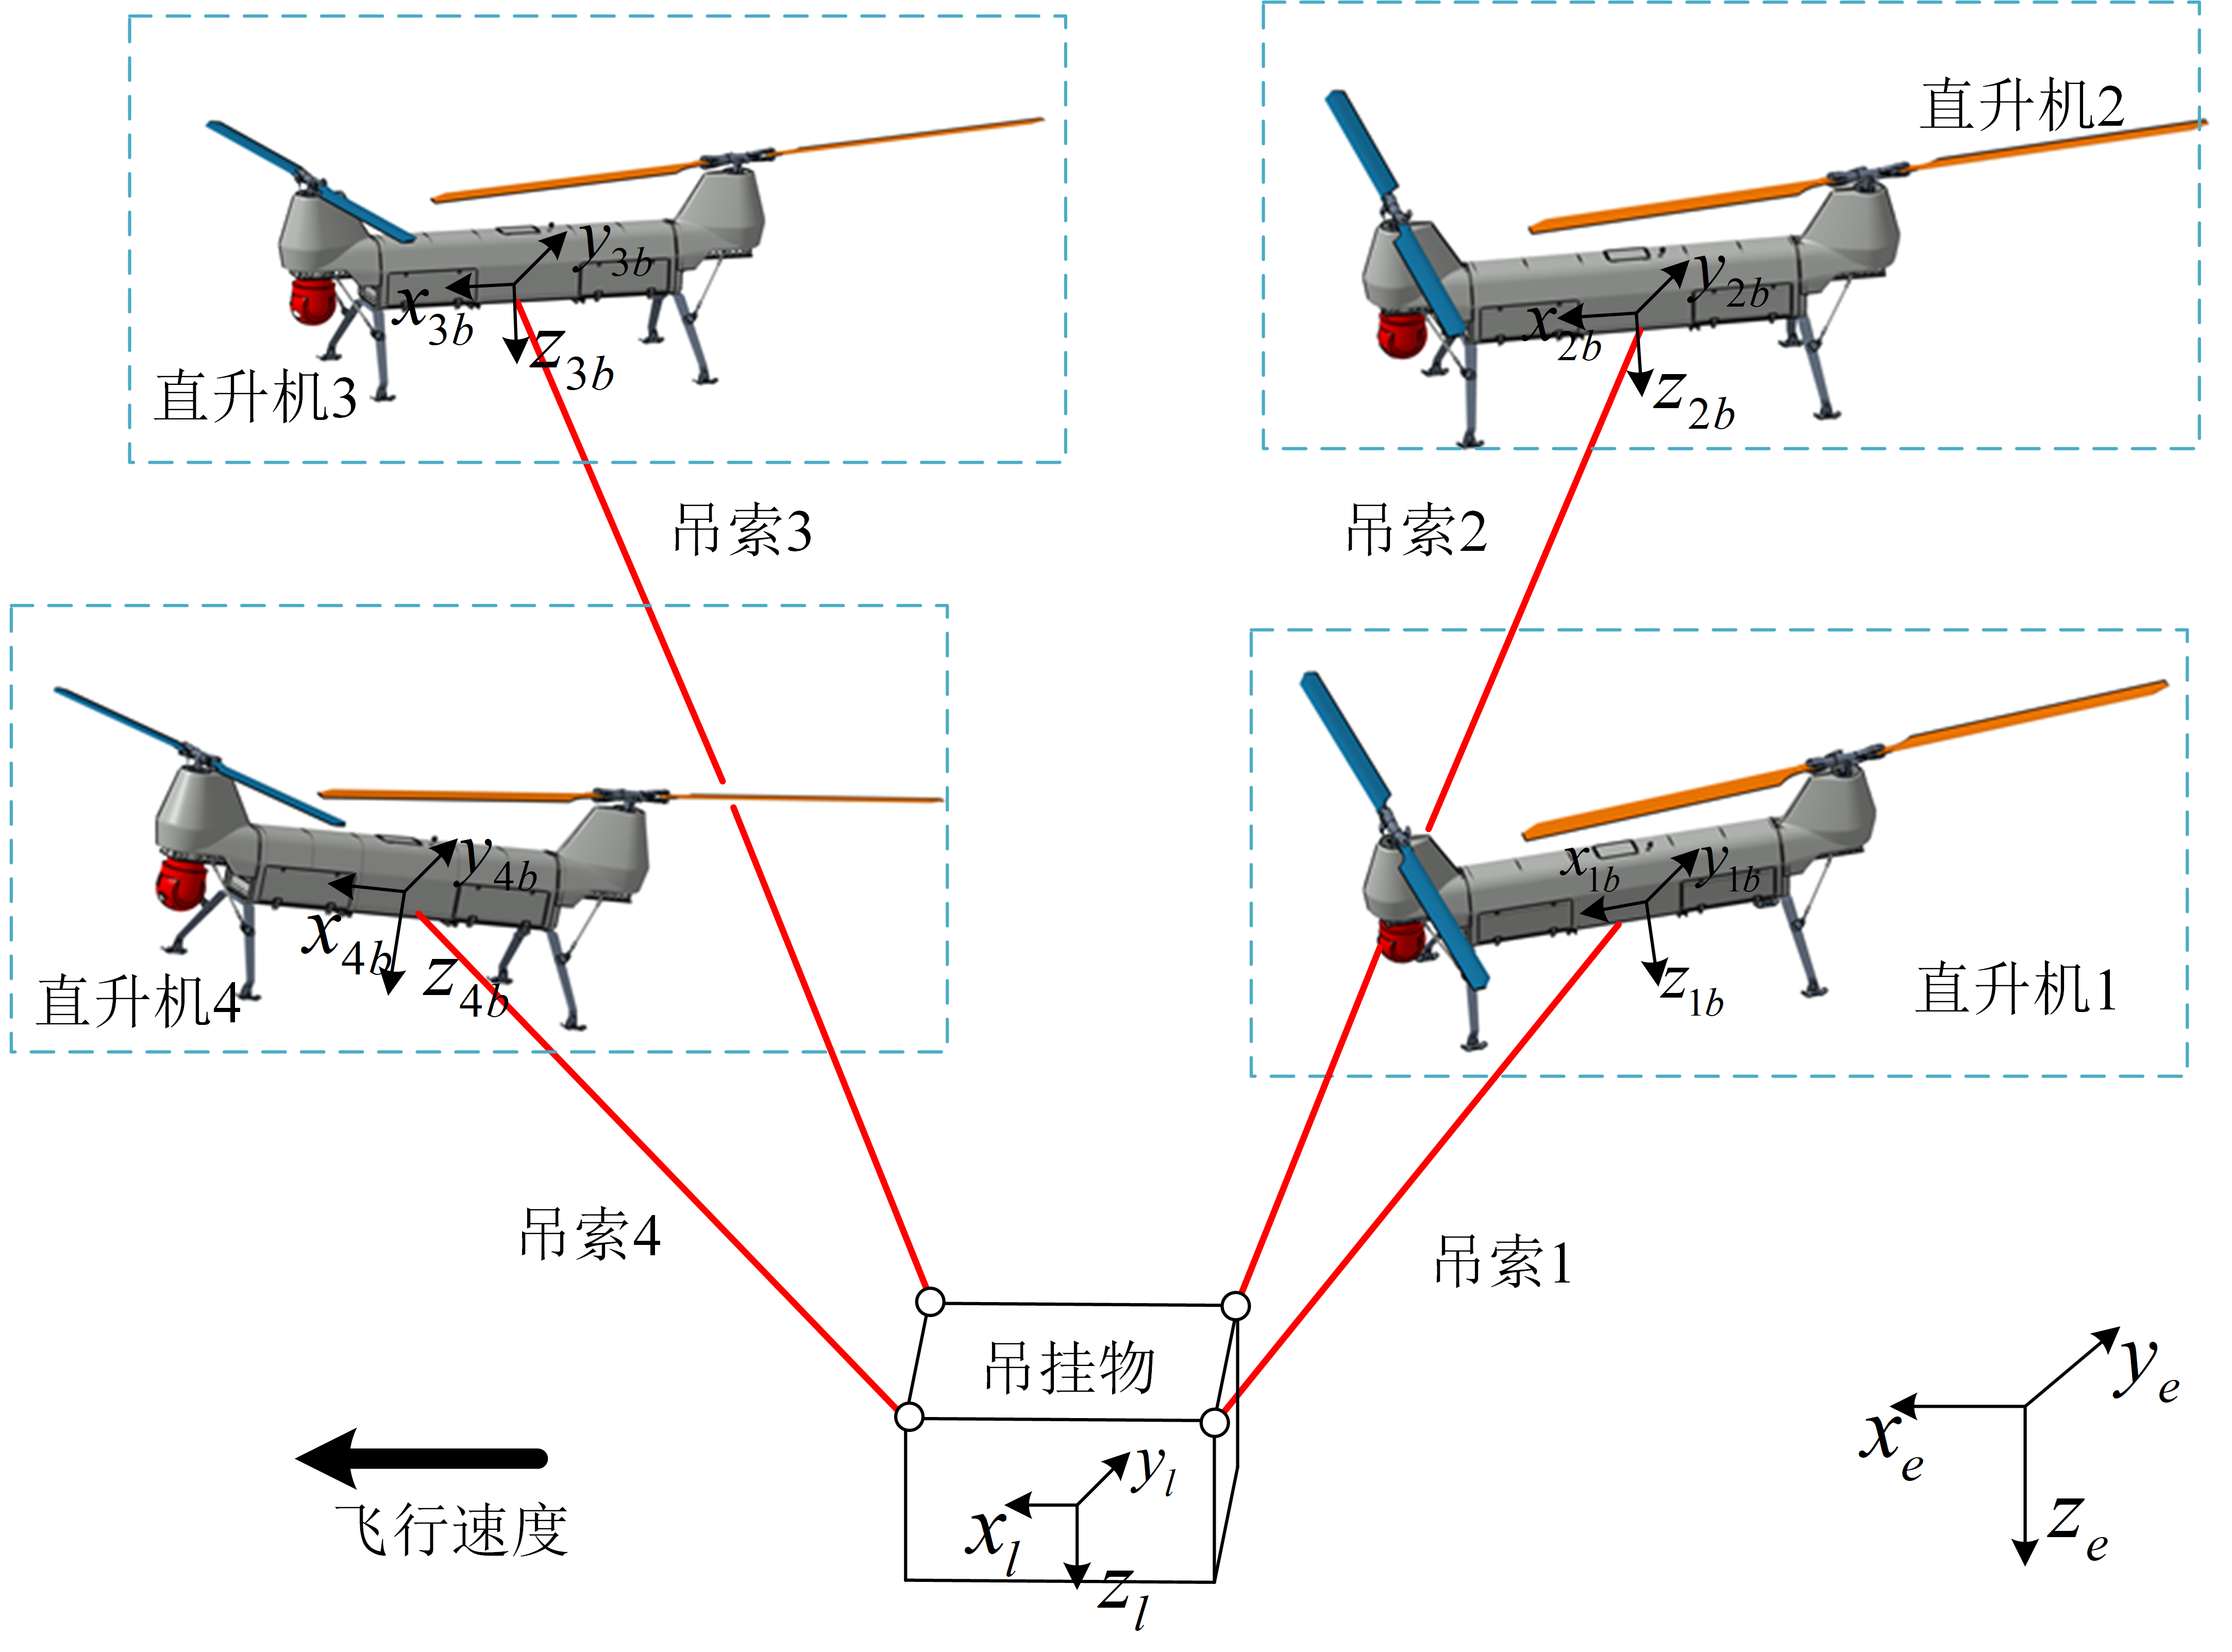
\includegraphics[width=10cm]{fig/figure_chap4/Chap4_1_2.png}
  \caption{本文研究对象:四纵列式直升机协同吊挂系统}
  \label{fig:4_1_2}
\end{figure}

本文研究的是“2-lead”队形的协同吊挂系统。见图\ref{fig:4_1_2},四个纵列式直升机各自采用7.2 m长的吊索协同吊挂负载。每个纵列式直升机有两副两片桨叶的旋翼,旋翼轴间的纵向距离为1.165 m,横向、垂向距离为0。旋翼旋转速度为113 rad/s,直径为1.8 m。负载是长方形的,其长、宽、高分别为1 m,0.4 m,0.4m。其重量为10 kg,大于单个直升机的运载能力(3.5 kg),小于整个协同吊挂系统的运载能力(14 kg)。此外,图\ref{fig:4_1_2}中,$x_ey_ez_e$、$x_{ib}y_{ib}z_{ib}$、$x_Ly_Lz_L$分别代表北-东-地的大地坐标系、直升机$i$的体轴系、吊挂物体轴系。

各个小型纵列式直升机的基本配置参数见下表。
\begin{table}[htb!]
  \caption{纵列式直升机基本配置参数}
  \begin{tabular}{cc}
    \toprule
    项目 & 数值 \\ 
    \midrule
    起飞重量(kg)& 15.0\\
    $I_{xx}\ (\rm{kg \cdot m^2})$ & 0.284 \\
    $I_{yy}\ (\rm{kg \cdot m^2})$ & 2.065 \\
    $I_{zz}\ (\rm{kg \cdot m^2})$ & 2.083 \\
    旋翼半径(m)& 0.9 \\
    桨叶弦长(m)& 0.069\\
    桨叶负扭( \degree )& 0\\
    桨叶片数 & 2\\
    旋翼转速(rad/s) & 113.1 \\
    前侧旋翼相对重心相对位置 & [0.5825, 0, -0.25]\\
    后侧旋翼相对重心相对位置 & [-0.5825, 0, -0.25]\\
    \bottomrule
  \end{tabular}
\end{table}
\section{研究目的及主要研究内容}
为提高直升机协同吊挂运输中的飞行品质和飞行安全,本课题着重研究直升机协同吊挂控制技术,意在达成五个方面的目标:
\begin{enumerate}
    \item 建立多直升机协同吊挂系统动力学模型并开展操稳特性分析:建立扩展性强(适应于单、双、多个直升机)、考虑气动干扰的直升机协同吊挂飞行动力学模型,形成针对吊挂物低阻尼特性的多直升机带吊挂系统混合配平优化算法,分析不同吊挂物质量、不同吊索长度、不同吊挂物模型等对直升机协同吊挂操稳特性的影响;
    \item 提出基于改进模型预测控制的直升机控制技术:在模型预测框架下,将直升机协同吊挂系统误差、环境不确定性、多机干涉等综合考虑到代价函数中,设计事件触发机制确定代价函数中各因素的权重,提出自适应调整预测时域方法来降低计算复杂度,基于卡尔曼滤波观测吊索力及系统误差补偿到控制输出中,然后将控制输出耦合输入整形技术,以抑制因直升机运动引发的吊挂物振荡;
    \item 提出基于博弈论的吊挂系统控制策略:在合作微分博弈框架下,建立吊挂系统的微分博弈模型,综合考虑各直升机性能、约束等,设计各吊索的性能函数,提出并性学习策略求解Hamilton-Jacobi方程,依据pareto最优求出最佳可行控制策略;
    \item 完成基于分层控制的直升机带吊挂系统轨迹跟踪及特情应对仿真:将基于改进模型预测控制的直升机控制技术和基于博弈的吊挂系统控制策略结合,形成以吊挂物为主导的分层控制策略,在此基础上完成多直升机带吊挂系统的轨迹跟踪及单机故障、突风时的特情应对仿真;
    \item 完成直升机协同吊挂系统试验试飞工作。
\end{enumerate}
% \chapter{直升机协同吊挂系统动力学建模}
\section{引言}
\section{直升机协同吊挂系统}
直升机协同吊挂系统一般包含两个或两个以上的直升机、若干吊索和一个吊挂物。
\section{坐标系及其转换关系}
在直升机协同吊挂系统建模过程中,用到了地心地固坐标系、经纬高地理坐标系、本地北东地(NED)坐标系、各直升机和吊挂物机载NED坐标系、各直升机和吊挂物体轴系、风轴系、直升机旋翼桨毂轴系、旋翼旋转轴系、中心铰坐标系和桨叶坐标系。为方便建模,本节首先给出了这些坐标系的详细定义及其转换关系。此外,考虑到控制系统设计时,各直升机及吊挂物姿态是用四元数表示的,本节最后还给出了四元数与欧拉角间的转换关系。
\subsection{坐标系}
\subsubsection{地心地固坐标系}
地心地固(Earth-Centered,Earth-Fixed)坐标系,简称ECEF坐标系,是一种笛卡尔直角坐标系,其坐标原点及坐标轴定义如下:
\begin{enumerate}
  \item 原点$O_{ECEF}$位于地球质心;
  \item $X$轴$X_{ECEF}$指向本初子午线与赤道的交点;
  \item $Y$轴$Y_{ECEF}$指向东经90 \degree 与赤道的交点;
  \item $Z$轴$Z_{ECEF}$指向地球北极点。
\end{enumerate}

ECEF坐标系定义见图\ref{ECEF}。其中$\gamma$表示地球经度,取值范围为-180 \degree 到180 \degree ;$\varphi$表示地球纬度,取值范围为-90 \degree 到90 \degree 。$R_a = 6378137.0 \rm{m}$表示地球长半轴,$R_b = 6356752.0 \rm{m}$表示地球短半轴。
此外,地球极扁率$f$、偏心率$e$、曲率半径$N$定义如下:
\begin{equation}
  \left\{ \begin{gathered}
    f = 1/298.257223565 \hfill \\
    e = \frac{{\sqrt {{R_a^2} - {R_b^2}} }}{R_a} \hfill \\
    N = \frac{R_a}{{\sqrt {1 - {e^2}{{\sin }^2}\varphi } }} \hfill \\ 
  \end{gathered}  \right.
\end{equation}
\begin{figure}[htb!]
  
\begin{tikzpicture}
    \draw (0,0) ellipse (3 and 2.8 );%画椭圆 
    \draw (0,0) ellipse (3 and 0.8) node[xshift = 1cm,yshift = -1cm]{赤道};%画椭圆 
    \draw (0,2.8) .. controls (-2, 1.5) and (-2,-1.5) .. (0,-2.8) node[left,xshift = -1.2cm, yshift = 4.5cm] {本初} node[left,xshift = -1.2cm, yshift = 4cm] {子午线};
    \draw[-latex] (0,0) -- (3.7,0) node[above] {$Y_{ECEF}$}; 
    \draw[-latex] (0,0) -- (0,3.5) node[right] {$Z_{ECEF}$} node[left, yshift = -0.5cm]{北极}; 
    \draw[-latex] (0,0) -- (-2.0,-1.0) node[below] {$X_{ECEF}$}; 
    \draw [green](-0.8,-0.4) -- (-0.8, 1.2);
    \draw [green](-0.8,1.2) -- (1.2, 1.2);
    \draw [green](1.2,1.2) -- (1.2, -0.4);
    \draw [green](1.2,-0.4) -- (2.0, 0);
    \draw [green](2.0, 0) -- (2.0, 1.6);
    \draw [green](2.0, 1.6) -- (0.0, 1.6);
    \draw [green](0.0, 1.6) -- (-0.8, 1.2); 
    \draw [green](-0.8,-0.4) -- (1.2, -0.4); 
    \draw [green](2.0, 1.6) -- (1.2, 1.2); 
    \draw[decorate,decoration={brace,amplitude=3mm},red] (0,0) -- (0,2.8) node[black,midway, xshift = -0.5cm] {$R_{b}$};
    \draw[decorate,decoration={brace,amplitude=3mm},red] (0,0) -- (3,0) node[black,midway,yshift = 0.5cm] {$R_{a}$};
    \draw [blue](0.0, 0) -- (1.2, -0.4);
    \draw [blue](0.3, -0.1) -- (1.25, 1.25);
    \draw
    (1.2, -0.4) coordinate (a)
    (0.3, -0.1) coordinate (b)
    (1.25, 1.25) coordinate (c)
    pic["$\varphi$", draw=orange, ->, angle eccentricity=1.2, angle radius=0.6cm]
    {angle=a--b--c};
    \draw
    (-2.0, -1.0) coordinate (a)
    (0.0, 0.0) coordinate (b)
    (1.2, -0.4) coordinate (c)
    pic["$\gamma$", draw=orange, ->, angle eccentricity=1.5, angle radius=0.3cm]
    {angle=a--b--c}; 
\end{tikzpicture}  



  \caption{ECEF坐标系及经纬度定义\label{ECEF}}
\end{figure}

\subsubsection{地理坐标系}
地理坐标系又称经纬高(LLA)坐标系,该坐标系下的位置向量定义如下:
\begin{equation}
  {\mathbf{P}}_g = \left[ \begin{gathered}
    \gamma  \hfill \\
    \varphi  \hfill \\
    h \hfill \\ 
  \end{gathered}  \right]
\end{equation}
其中,$\gamma$、$\varphi$定义见图\ref{ECEF},$h$为飞行器与参考椭球面间的垂向距离。

\subsubsection{本地北东地NED坐标系}
见图\ref{NED},本地北东地NED坐标系,与地面固连,其坐标原点及坐标轴定义如下:
\begin{enumerate}
  \item 坐标原点$O_e$为固连在地面上的任一点;
  \item $X$轴$X_{e}$指向地理北极;
  \item $Y$轴$Y_{e}$指向地理东方;
  \item $Z$轴$Z_{e}$沿地球椭球面法线指向下。
\end{enumerate}

\subsubsection{机载北东地NED坐标系}
本地北东地NED坐标系,与飞行器固连,其坐标轴指向会随着飞行器运动而改变。坐标原点及坐标轴定义如下:
\begin{enumerate}
  \item 坐标原点$O_{ev}$位于飞行器质心;
  \item $X$轴$X_{ev}$指向地理北极;
  \item $Y$轴$Y_{ev}$指向地理东方;
  \item $Z$轴$Z_{ev}$沿地球椭球面法线指向上。
\end{enumerate}

\begin{figure}[htb!]
  % \documentclass{article}
% \usepackage{xeCJK}
% \usepackage{tikz}
% \usetikzlibrary{decorations.pathreplacing, calligraphy}
% \usetikzlibrary{quotes,angles}
% \begin{document}
\begin{tikzpicture}
    \node at (0,0) {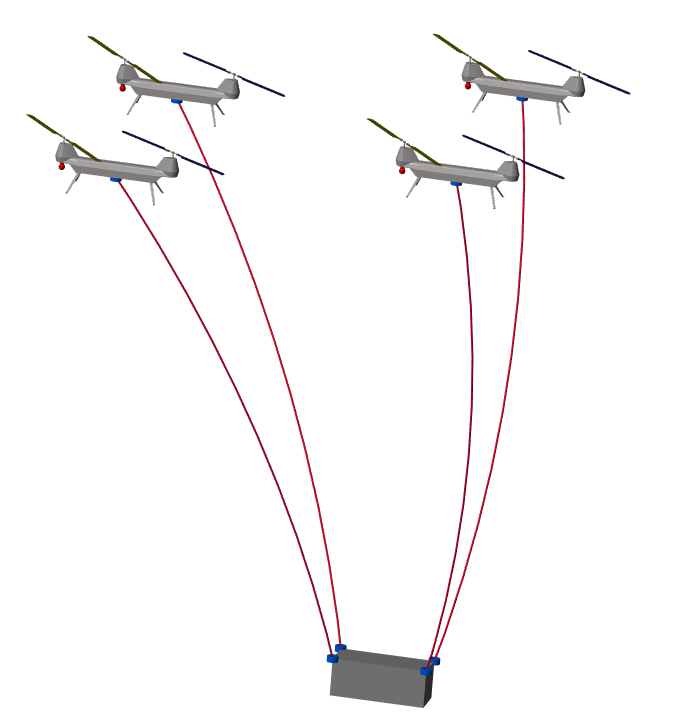
\includegraphics[width = 7cm]{multi_lift.PNG}};
    \draw[-latex] (-2,-2) -- (-3.7,-2) node[above] {飞行方向}; 
    \draw[-latex] (5,-2.5) -- (4,-2.5) node[above] {$X_e$};
    \draw[-latex] (5,-2.5) -- (5.5,-2) node[above] {$Y_e$}; 
    \draw[-latex] (5,-2.5) -- (5,-3.5) node[left] {$Z_e$}; 
    \draw (5,-2.5) node[right, yshift = -0.2cm]{$O_e$};

    \draw[-latex] (0.4,-3.25) -- (-0.5,-3.25) node[below] {$X_{ev,l}$};
    \draw[-latex] (0.4,-3.25) -- (0.9,-2.5) node[left] {$Y_{ev,l}$}; 
    \draw[-latex] (0.4,-3.25) -- (0.4,-4) node[left] {$Z_{ev,l}$}; 
    \draw (0.4,-3.25) node[right, yshift = -0.2cm]{$O_{ev,l}$};

    \draw[-latex] (1.2,1.95) -- (0.5,1.95) node[below] {$X_{ev,1}$};
    \draw[-latex] (1.2,1.95) -- (1.7,2.4) node[left] {$Y_{ev,1}$}; 
    \draw[-latex] (1.2,1.95) -- (1.2,1.2) node[right] {$Z_{ev,1}$}; 
    \draw (1.2,1.95) node[right, yshift = -0.2cm]{$O_{ev,1}$};

\end{tikzpicture}  

% \end{document}
  \caption{本地和机载NED坐标系定义\label{NED}}
\end{figure}

为方便论述,直升机$i$的机载NED坐标系定义为$OXYZ_{ev,i}$,吊挂物的机载NED坐标系定义为$OXYZ_{ev,l}$。图\ref{NED}以四个纵列式直升机协同吊挂为例,给出了吊挂物和直升机1的机载NED坐标系。

\subsubsection{机体坐标系}
机体坐标系又称体轴系,与飞行器固连,用于确定飞行器在空中的姿态,其坐标原点及坐标轴定义如下:
\begin{enumerate}
  \item 坐标原点$O_{b}$位于飞行器质心;
  \item $X$轴$X_{b}$位于飞行器纵向对称面内,指向前;
  \item $Y$轴$Y_{b}$垂直于飞行器纵向对称面,指向右;
  \item $Z$轴$Z_{b}$位于飞行器纵向对称面内,垂直于$X_{b}$轴指向下。
\end{enumerate}

为方便论述,直升机$i$的机体坐标系定义为$OXYZ_{b,i}$,吊挂物机体坐标系定义为$OXYZ_{b,l}$。

\subsubsection{风轴系}
风轴系也叫速度轴系,直升机$i$的风轴系定义为$OXYZ_{V,i}$,吊挂物风轴系定义为$OXYZ_{V,l}$。其坐标原点及坐标轴定义如下:
\begin{enumerate}
  \item 坐标原点$O_V$位于飞行器质心;
  \item $X$轴$X_{V}$沿飞行速度方向;
  \item $Z$轴$Z_{V}$在飞行器纵向对称面内垂直$X_{V}$指向下;
  \item $Y$轴$Y_{V}$由右手定则确定。
\end{enumerate}

\subsubsection{旋翼桨毂轴系}
旋翼桨毂轴系与旋翼桨毂中心固连,其坐标原点及坐标轴定义如下
\begin{enumerate}
  \item 坐标原点$O_h$位于旋翼桨毂中心;
  \item $Z$轴($Z_h$)平行于旋翼轴指向上;
  \item $X$轴($X_h$)位于桨毂平面内且垂直于$Z_h$轴指向后;
  \item 若为右旋旋翼,$Y$轴($Y_h$)由右手定则确定;若为左旋旋翼,$Y$轴($Y_h$)由左手定则确定。
\end{enumerate}
\subsubsection{旋翼旋转轴系}
旋翼旋转轴系记为$OXYZ_r$,其坐标原点及坐标轴定义如下
\begin{enumerate}
  \item 坐标原点$O_r$位于桨毂中心处;
  \item $X$轴($X_r$)为$X_h$轴绕旋翼转向旋转一定方位角后的指向,$X_h$轴初始方位为0 \degree 方位角;
  \item $Z$轴($Z_r$)平行于旋翼轴指向上;
  \item 若为右旋旋翼,$Y$轴($Y_r$)由右手定则确定;若为左旋旋翼,$Y$轴($Y_r$)由左手定则确定。
\end{enumerate}
\subsubsection{桨叶坐标系}
本文中旋翼模型不涉及旋翼的摆振运动,所以相比其他文献,无需定义中心铰坐标系。桨叶坐标系的坐标原点和坐标轴定义如下:
\begin{enumerate}
  \item 坐标原点$O_{bl}$位于挥舞铰上;
  \item $X$轴($X_{bl}$)沿桨叶径向指向外;
  \item $Z$轴($Y_{bl}$)在桨叶挥舞平面内垂直于($X_{bl}$)轴指向上;
  \item 若为右旋旋翼,$Y$轴($Y_{bl}$)由右手定则确定;若为左旋旋翼,$Y$轴($Y_{bl}$)由左手定则确定。
\end{enumerate}
\subsubsection{叶素坐标系}
将桨叶分为$n$个叶素段,则第$i$个叶素的坐标系定义为
\begin{enumerate}
  \item 坐标原点$O_{el,i}$位于第$i$个叶素段中心处;
  \item $X$轴($X_{el,i}$)沿叶素弦线指向前;
  \item $Z$轴($Z_{el,i}$)在叶素对称面内垂直于叶素弦线指向下;
  \item 若为右旋旋翼,$Y$轴($Y_{el,i}$)由右手定则确定;若为左旋旋翼,$Y$轴($Y_{el,i}$)由左手定则确定。
\end{enumerate}
\subsection{坐标系间的转换关系}
为方便下文论述,本节给出了LLA坐标系与ECEF坐标系间的转换关系,ECEF坐标系与NED坐标系间的转换关系、NED坐标系与体轴系间的转换关系、风轴系与体轴系间的转换关系以及欧拉角与四元数间的转换关系。
\subsubsection{LLA坐标系与ECEF坐标系间的转换关系}
\begin{enumerate}
  \item 设LLA坐标系下一点坐标为$(\gamma, \varphi, h)$,则ECEF坐标系下对应坐标为
  \begin{equation}
    \left\{ \begin{gathered}
      {X_{ECEF}} = \left( {N + h} \right)\cos \left( \varphi  \right)\cos \left( \gamma  \right) \hfill \\
      {Y_{ECEF}} = \left( {N + h} \right)\cos \left( \varphi  \right)\sin \left( \gamma  \right) \hfill \\
      {Z_{ECEF}} = \left( {N\left( {1 - {e^2}} \right) + h} \right)\sin \left( \varphi  \right) \hfill \\ 
    \end{gathered}  \right.
  \end{equation}
  \item 反之,ECEF坐标系到LLA坐标系间的转换关系为:
  \begin{equation}
    \left\{ \begin{gathered}
      \gamma  = \arctan \left( {\frac{{{Y_{ECEF}}}}{{{X_{ECEF}}}}} \right) \hfill \\
      \varphi {\text{ = }}\arctan \left( {\frac{Z_{ECEF}}{p}{{\left( {1 - {e^2}\frac{N}{{N + h}}} \right)}^{ - 1}}} \right) \hfill \\
      h = \frac{p}{{\cos \left( \varphi  \right) - N}} \hfill \\ 
    \end{gathered}  \right.
  \end{equation}
  其中,$p = \sqrt{X_{ECEF}^2 + Y_{ECEF}^2}$
\end{enumerate}
\subsubsection{ECEF坐标系与本地NED坐标系间的转换关系}
\begin{enumerate}
  \item 设本地ECEF坐标系原点为$P_{ECEF,0} = (X_{ECEF,0}, Y_{ECEF,0}, Z_{ECEF,0})$,对应的LLA坐标点为$(\gamma_0, \varphi_0, h_0)$。计算点$P_{ECEF}$在ECEF坐标系下的坐标点为$(X_{ECEF}, Y_{ECEF}, Z_{ECEF})$。则$P_{ECEF}$在以$P_{ECEF,0}$为坐标原点的NED坐标系下的坐标为:
  \begin{equation}
    \left[ \begin{gathered}
      n \hfill \\
      e \hfill \\
      d \hfill \\ 
    \end{gathered}  \right] = \underbrace {\left[ {\begin{array}{*{20}{c}}
      { - \sin \left( {{\varphi _0}} \right)\cos \left( {{\gamma _0}} \right)}&{ - \sin \left( {{\varphi _0}} \right)\sin \left( {{\gamma _0}} \right)}&{\cos \left( {{\varphi _0}} \right)} \\ 
      { - \sin \left( {{\gamma _0}} \right)}&{\cos \left( {{\gamma _0}} \right)}&0 \\ 
      {-\cos \left( {{\varphi _0}} \right)\cos \left( {{\gamma _0}} \right)}&{-\cos \left( {{\varphi _0}} \right)\sin \left( {{\gamma _0}} \right)}&{-\sin \left( {{\varphi _0}} \right)} 
    \end{array}} \right]}_S\left[ \begin{gathered}
      \Delta x \hfill \\
      \Delta y \hfill \\
      \Delta z \hfill \\ 
    \end{gathered}  \right]
  \end{equation}
  其中,$\Delta x = X_{ECEF} - X_{ECEF,0}$,$\Delta y = Y_{ECEF} - Y_{ECEF,0}$,$\Delta z = Z_{ECEF} - Z_{ECEF,0}$。
  \item 反之,
  \begin{equation}
    \left[ \begin{gathered}
      \Delta x \hfill \\
      \Delta y \hfill \\
      \Delta z \hfill \\ 
    \end{gathered}  \right] = {S^{ - 1}}\left[ \begin{gathered}
      n \hfill \\
      e \hfill \\
      d \hfill \\ 
    \end{gathered}  \right]
  \end{equation}
\end{enumerate}

\subsubsection{机载NED坐标系与体轴系间的转换关系}
机载NED坐标系依次绕Z-Y-X轴做欧拉旋转,得到体轴系。以直升机$i$为例,坐标系$OXYZ_{ev,i}$与坐标系$OXYZ_{b,i}$之间的转换关系为
\begin{equation}
  \left[ \begin{gathered}
    {X_{b,i}} \hfill \\
    {Y_{b,i}} \hfill \\
    {Z_{b,i}} \hfill \\ 
  \end{gathered}  \right] = \underbrace {\underbrace {\left[ {\begin{array}{*{20}{c}}
    1&0&0 \\ 
    0&{\cos {\phi _i}}&{\sin {\phi _i}} \\ 
    0&{ - \sin {\phi _i}}&{\cos {\phi _i}} 
  \end{array}} \right]}_{{{\mathbf{R}}_x}}\underbrace {\left[ {\begin{array}{*{20}{c}}
    {\cos {\theta _i}}&0&{ - \sin {\theta _i}} \\ 
    0&1&0 \\ 
    {\sin {\theta _i}}&0&{\cos {\theta _i}} 
  \end{array}} \right]}_{{{\mathbf{R}}_y}}\underbrace {\left[ {\begin{array}{*{20}{c}}
    {\cos {\psi _i}}&{\sin {\psi _i}}&0 \\ 
    { - \sin {\psi _i}}&{\cos {\psi _i}}&0 \\ 
    0&0&1 
  \end{array}} \right]}_{{{\mathbf{R}}_z}}}_{{{\mathbf{R}}_{bi/evi}}}\left[ \begin{gathered}
    {X_{ev,i}} \hfill \\
    {Y_{ev,i}} \hfill \\
    {Z_{ev,i}} \hfill \\ 
  \end{gathered}  \right]
\end{equation}
其中,$\mathbf{R}_{bi/evi}$称为直升机$i$机载NED坐标系到体轴系的转换矩阵。

此外,
\begin{enumerate}
  \item 偏航角$\psi_i$为机载坐标系绕$Z$轴旋转过的角度,即机载NED坐标系$X_{ev,i}$轴与体轴系$X_{b,i}$轴在机载NED坐标系$X_{ev,i}Y_{ev,i}$平面的投影,经过$\mathbf{R}_z$转换后得到中间坐标系;
  \item 俯仰角$\theta_i$为中间坐标系绕$Y$轴旋转过的角度,经过$\mathbf{R}_y$转换后得到二次中间坐标系;
  \item 滚转角$\phi_i$为二次中间坐标系绕$X$轴旋转的角度,旋转矩阵记作$\mathbf{R}_x$。
\end{enumerate}

图\ref{body}以直升机1为例,给出了机载NED坐标系与体轴系的转换关系及姿态角定义。

\begin{figure}[htb!]
  \subfloat[绕$Z$轴旋转]{% \documentclass{article}
% \usepackage{xeCJK}
% \usepackage{tikz}
% \usetikzlibrary{decorations.pathreplacing, calligraphy}
% \usetikzlibrary{quotes,angles}
% \begin{document}
\begin{tikzpicture}
    \node at (0,0) {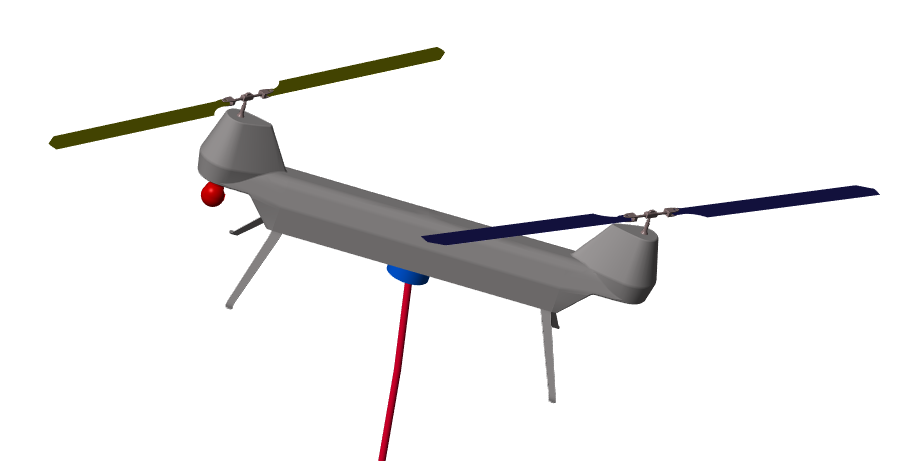
\includegraphics[width = 5cm]{tandem.PNG}};
    \draw[-latex] (-1,-2) -- (-2.5,-2) node[above] {飞行方向}; 
    %机载NED坐标系 
    \draw[-latex] (-0.3,-0.1) -- (-3.,-0.1) node[below] {$X_{ev,1}$};
    \draw[-latex] (-0.3,-0.1) -- (1.0,1.5) node[left] {$Y_{ev,1}$}; 
    \draw[-latex] (-0.3,-0.1) -- (-0.3,-2) node[right,yshift = 0.5cm] {$Z_{ev,1}$}; 
    \draw (-0.3,-0.1) node[right, yshift = -0.2cm]{$O_{ev,1}$} node[right, yshift = -0.6cm]{$O_{b,1}^z$};
    % 绕z轴旋转后的坐标系
    \draw[-latex] (-0.3,-0.1) -- (-3.,0.35) node[above] {$X_{b,1}^z$};
    \draw[-latex] (-0.3,-0.1) -- (1.5,1.4) node[right] {$Y_{b,1}^z$}; 
    \draw[-latex] (-0.3,-0.1) -- (-0.3,-2) node[right] {$Z_{b,1}^z$}; 
    \draw
    (-3.,0.35) coordinate (a)
    (-0.3, -0.1) coordinate (b)
    (-3.,-0.1) coordinate (c)
    pic["$\psi_1$", draw=orange, <-, angle eccentricity=1.2, angle radius=1.8cm]
    {angle=a--b--c};
\end{tikzpicture}  

% \end{document}}\quad
  \subfloat[绕$Y$轴旋转]{% \documentclass{article}
% \usepackage{xeCJK}
% \usepackage{tikz}
% \usetikzlibrary{decorations.pathreplacing, calligraphy}
% \usetikzlibrary{quotes,angles}
% \begin{document}
\begin{tikzpicture}
    \node at (0,0) {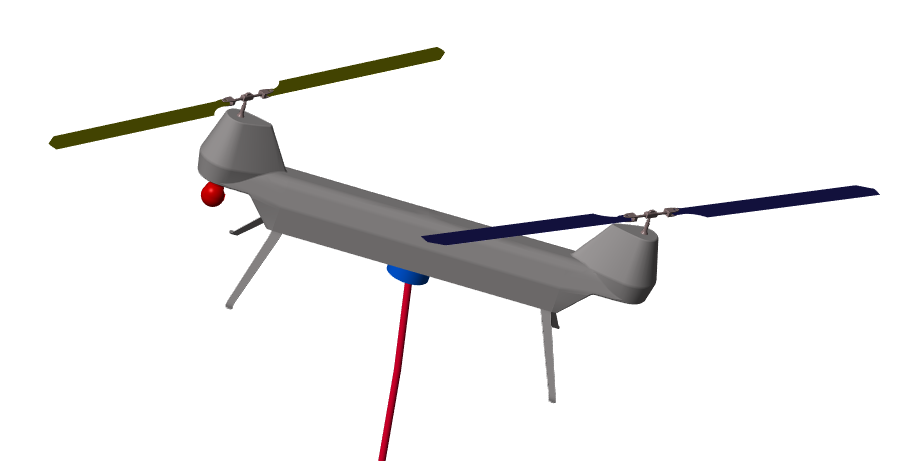
\includegraphics[width = 5cm]{tandem.PNG}};
    \draw[-latex] (-1,-2) -- (-2.5,-2) node[above] {飞行方向}; 
    \draw (-0.3,-0.1) node[right, yshift = -0.2cm]{$O_{b,1}^z$} node[right, yshift = -0.6cm]{$O_{b,1}^{y}$};
    % 绕z轴旋转
    \draw[-latex] (-0.3,-0.1) -- (-3.,0.35) node[below] {$X_{b,1}^z$};
    \draw[-latex] (-0.3,-0.1) -- (1.5,1.4) node[right] {$Y_{b,1}^z$}; 
    \draw[-latex] (-0.3,-0.1) -- (-0.3,-2) node[right] {$Z_{b,1}^z$}; 
    % 绕y轴旋转
    \draw[-latex] (-0.3,-0.1) -- (-3.,0.7) node[above] {$X_{b,1}^y$};
    \draw[-latex] (-0.3,-0.1) -- (1.5,1.4) node[right, yshift = -0.5cm] {$Y_{b,1}^y$}; 
    \draw[-latex] (-0.3,-0.1) -- (-0.65,-2) node[left,yshift = 0.4cm] {$Z_{b,1}^y$}; 
    \draw
    (-3.,0.7) coordinate (a)
    (-0.3, -0.1) coordinate (b)
    (-3.,0.35) coordinate (c)
    pic["$\theta_1$", draw=orange, <-, angle eccentricity=1.2, angle radius=1.8cm]
    {angle=a--b--c};
\end{tikzpicture}  

% \end{document}}
  \subfloat[绕$X$轴旋转]{% \documentclass{article}
% \usepackage{xeCJK}
% \usepackage{tikz}
% \usetikzlibrary{decorations.pathreplacing, calligraphy}
% \usetikzlibrary{quotes,angles}
% \begin{document}
\begin{tikzpicture}
    \node at (0,0) {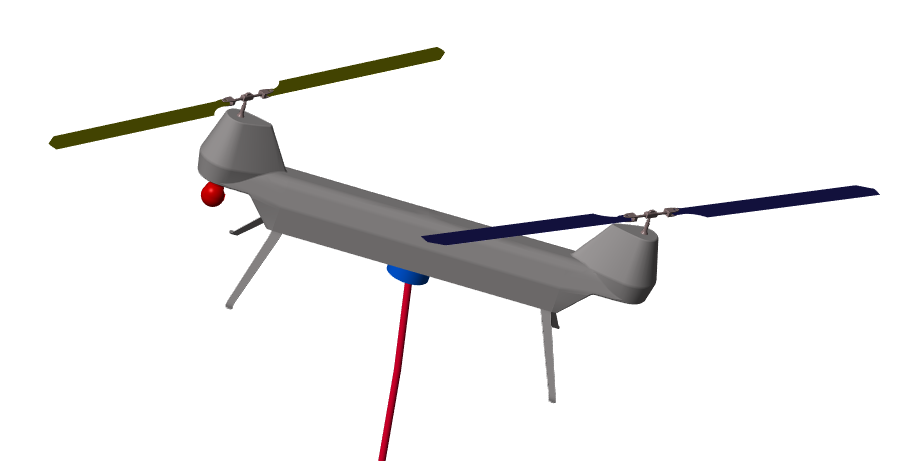
\includegraphics[width = 5cm]{tandem.PNG}};
    \draw[-latex] (-1,-2) -- (-2.5,-2) node[above] {飞行方向}; 
    \draw (-0.3,-0.1) node[right, yshift = -0.2cm]{$O_{b,1}^y$} node[right, yshift = -0.6cm]{$O_{b,1}$};
    % 绕y轴旋转
    \draw[-latex] (-0.3,-0.1) -- (-3.,0.7) node[above] {$X_{b,1}^y$};
    \draw[-latex] (-0.3,-0.1) -- (1.5,1.4) node[right] {$Y_{b,1}^y$}; 
    \draw[-latex] (-0.3,-0.1) -- (-0.65,-2) node[right,yshift = 0.4cm] {$Z_{b,1}^y$}; 
     % 绕x轴旋转
     \draw[-latex] (-0.3,-0.1) -- (-3.,0.7) node[below] {$X_{b,1}$};
     \draw[-latex] (-0.3,-0.1) -- (1.5,1.0) node[right] {$Y_{b,1}$}; 
     \draw[-latex] (-0.3,-0.1) -- (-0.95,-1.9) node[left,yshift = 0.4cm] {$Z_{b,1}$};   
     \draw
    (1.5,1.0) coordinate (a)
    (-0.3, -0.1) coordinate (b)
    (1.5,1.4) coordinate (c)
    pic["$\phi_1$", draw=orange, <-, angle eccentricity=1.2, angle radius=1.5cm]
    {angle=a--b--c};
\end{tikzpicture}  

% \end{document}}
  \caption{机载NED坐标系转到体轴系及姿态角定义\label{body}}
\end{figure}

\subsubsection{风轴系与体轴系间的转换关系}
定义侧滑角$\beta$为速度矢量与$X_bO_bY_b$平面夹角,右侧滑为正。迎角$\alpha$为速度矢量在$X_bO_bZ_b$平面的投影与$O_bX_b$轴的夹角,速度矢量在$X_bO_bY_b$平面下方时迎角为正。

风轴系与体轴系间的转换关系为
\begin{equation}
  \left[ \begin{gathered}
    {X_b} \hfill \\
    {Y_b} \hfill \\
    {Z_b} \hfill \\ 
  \end{gathered}  \right] = \underbrace {\underbrace {\left[ {\begin{array}{*{20}{c}}
    {\cos \alpha }&0&{ - \sin \alpha } \\ 
    0&1&0 \\ 
    {\sin \alpha }&0&{\cos \alpha } 
  \end{array}} \right]}_{{{\mathbf{R}}_\alpha }}\underbrace {\left[ {\begin{array}{*{20}{c}}
    {\cos \beta }&{ - \sin \beta }&0 \\ 
    {\sin \beta }&{\cos \beta }&0 \\ 
    0&0&1 
  \end{array}} \right]}_{{{\mathbf{R}}_\beta }}}_{{{\mathbf{R}}_{b/V}}}\left[ \begin{gathered}
    {X_V} \hfill \\
    {Y_V} \hfill \\
    {Z_V} \hfill \\ 
  \end{gathered}  \right]
\end{equation}

\begin{figure}[htb!]
  \subfloat[桨轴前倾角]{% \documentclass{article}
% \usepackage{xeCJK}
% \usepackage{tikz}
% \usetikzlibrary{decorations.pathreplacing, calligraphy}
% \usetikzlibrary{quotes,angles}
% \begin{document}
\begin{tikzpicture}
    % 体轴系
    \draw[-latex] (-0.3,-0.1) -- (-3.,-0.1) node
    [above] {$X_{b,1}$};
    \draw[-latex] (-0.3,-0.1) -- (1.5,1.4) node[right] {$Y_{b,1}$}; 
    \draw[-latex] (-0.3,-0.1) -- (-0.3,-2) node[right] {$Z_{b,1}$}; 
    %桨毂轴系
    \draw[-latex] (-0.3,-0.1) -- (2.5,0.5) node[above] {$X_{h}$};
    \draw[-latex] (-0.3,-0.1) -- (1.5,1.4) node[right,yshift = 0.4cm] {$Y_{h}$}; 
    \draw[-latex] (-0.3,-0.1) -- (-0.8,2) node[left] {$Z_{h}$};
    % 辅助线
    \draw[dash dot](-0.3,-0.1) -- (2.5,-0.1);
    \draw[dash dot](-0.3,-0.1) -- (-0.3,2);
    \draw
    (-0.3,2) coordinate (a)
    (-0.3, -0.1) coordinate (b)
    (-0.8,2) coordinate (c)
    pic["$\delta$", draw=orange, ->, angle eccentricity=1.2, angle radius=1.5cm]
    {angle=a--b--c};
\end{tikzpicture}  

% \end{document}}\quad
  \subfloat[旋翼旋转轴系]{% \documentclass{article}
% \usepackage{xeCJK}
% \usepackage{tikz}
% \usetikzlibrary{decorations.pathreplacing, calligraphy}
% \usetikzlibrary{quotes,angles}
% \begin{document}
\begin{tikzpicture}
    \node at (1.1,-1.3) {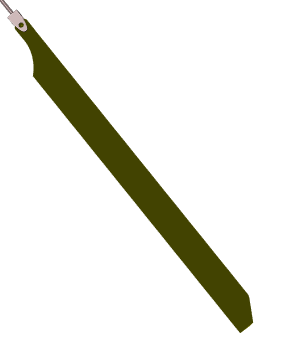
\includegraphics[width = 2.2cm]{blade.png}};
    \draw[dash dot](-2,0)--(1,0);
    \draw[dash dot](0,-2)--(0,1);
    \draw[-latex] -> (0,0)--(0,-3.0) node[left]{$X_h$};
    \draw[-latex] -> (0,0)--(1.8,0) node[above]{$Y_h$};
    \draw[-latex] -> (0,0)--(2.14,-2.7) node[left]{$X_r$};
    \draw[-latex] -> (0,0)--(1.5,1.1) node[above]{$Y_r$};
    \draw 
    (0,-4)coordinate(a)
    (0,0)coordinate(b)
    (2.14,-2.7)coordinate(c)
    pic["$\psi_r$", draw=orange, ->, angle eccentricity=1.2, angle radius=1.5cm]
    {angle=a--b--c};

\end{tikzpicture}  

% \end{document}}\quad
  \subfloat[桨叶坐标系]{% \documentclass{article}
% \usepackage{xeCJK}
% \usepackage{tikz}
% \usetikzlibrary{decorations.pathreplacing, calligraphy}
% \usetikzlibrary{quotes,angles}
% \begin{document}
\begin{tikzpicture}
    \node at (0,0) {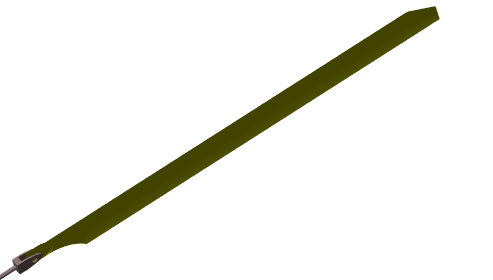
\includegraphics[width = 3cm]{blade1.png}};
    \draw[-latex](-1.5,-0.85)--(2,-0.85) node[below]{$X_r$};
    \draw[-latex](-1.5,-0.85)--(-1.5,1) node[above]{$Z_r$};
    \draw[-latex](-1.5,-0.85)--(1.8,1.25) node[above]{$X_{bl}$};
    \draw[-latex](-1.5,-0.85)--(-2.6,1) node[left]{$Z_{bl}$};
    \draw 
    (2,-0.85)coordinate(a)
    (-1.5,-0.85)coordinate(b)
    (1.8,1.25)coordinate(c)
    pic["$\beta_{bl}$", draw=orange, ->, angle eccentricity=1.2, angle radius=1.5cm]
    {angle=a--b--c};

\end{tikzpicture}  

% \end{document}}\quad\quad
  \subfloat[叶素坐标系]{% \documentclass{article}
% \usepackage{xeCJK}
% \usepackage{tikz}
% \usetikzlibrary{decorations.pathreplacing, calligraphy}
% \usetikzlibrary{quotes,angles}
% \begin{document}
\begin{tikzpicture}
    \node at (0,0) {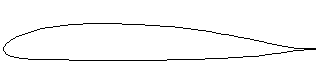
\includegraphics[width = 4cm, angle = -30]{OA212.png}};
    \draw[-latex](-0.5,0.2)--(-2.5,0.2) node[below]{$Y_{bl}$};
    \draw[-latex](-0.5,0.2)--(-0.5,2) node[left]{$Z_{bl}$};
    \draw[-latex](-0.5,0.2)--(-2.5,1.2) node[above]{$X_{el,i}$};
    \draw[-latex](-0.5,0.2)--(-1.1,-1.2) node[left]{$Z_{el,i}$};
    \draw 
    (-2.5,1.2)coordinate(a)
    (-0.5,0.2)coordinate(b)
    (-2.5,0.2)coordinate(c)
    pic["$\theta_{el,i}$", draw=orange, <-, angle eccentricity=1.2, angle radius=1.5cm]
    {angle=a--b--c};

\end{tikzpicture}  

% \end{document}}
  \caption{体轴系、桨毂轴系、旋翼旋转轴系、桨叶坐标系、叶素坐标系间的转换关系\label{rotor}}
\end{figure}
\subsubsection{体轴系与桨毂轴系间的转换关系}
定义桨轴前倾角为$\delta$,见图\ref{rotor}(a)。以右旋旋翼为例,体轴系与桨毂轴系间的欧拉角为$(0, \pi-\delta, 0)$,对应的转换关系为
\begin{equation}
  \left[ \begin{gathered}
    {X_h} \hfill \\
    {Y_h} \hfill \\
    {Z_h} \hfill \\ 
  \end{gathered}  \right] = \underbrace {\left[ {\begin{array}{*{20}{c}}
    {\cos \delta }&0&{\sin \delta } \\ 
    0&1&0 \\ 
    { - \sin \delta }&0&{\cos \delta } 
  \end{array}} \right]\left[ {\begin{array}{*{20}{c}}
    { - 1}&0&0 \\ 
    0&1&0 \\ 
    0&0&{ - 1} 
  \end{array}} \right]}_{{{\mathbf{R}}_{h/b}}}\left[ \begin{gathered}
    {X_b} \hfill \\
    {Y_b} \hfill \\
    {Z_b} \hfill \\ 
  \end{gathered}  \right]
\end{equation}
\subsubsection{桨毂轴系与旋翼旋转轴系间的转换关系}
在方位角为$\psi_r$时,见图\ref{rotor}(b),旋翼桨毂轴系与旋转轴系之间的欧拉角为$(0, 0, \psi_r)$,对应的转换关系为
\begin{equation}
  \left[ \begin{gathered}
    {X_{r}} \hfill \\
    {Y_{r}} \hfill \\
    {Z_{r}} \hfill \\ 
  \end{gathered}  \right] = \underbrace {\left[ {\begin{array}{*{20}{c}}
    \cos \psi_r&\sin \psi_r&0 \\ 
    -\sin \psi_r&\cos \psi_r&0 \\ 
    0&0&1
  \end{array}} \right]}_{{{\mathbf{R}}_{r/h}}}\left[ \begin{gathered}
    {X_h} \hfill \\
    {Y_h} \hfill \\
    {Z_h} \hfill \\ 
  \end{gathered}  \right]
\end{equation}

\subsubsection{旋翼旋转轴系与桨叶坐标系间的转换关系}
当挥舞角为$\beta_{bl}$时,见图\ref{rotor}(c),旋翼旋转轴系与桨叶坐标系间的欧拉角为$(0, -\beta_{bl}, 0)$,对应的转换关系为
\begin{equation}
  \left[ \begin{gathered}
    {X_{bl}} \hfill \\
    {Y_{bl}} \hfill \\
    {Z_{bl}} \hfill \\ 
  \end{gathered}  \right] = \underbrace {\left[ {\begin{array}{*{20}{c}}
    {\cos {\beta _{bl}}}&0&{\sin {\beta _{bl}}} \\ 
    0&1&0 \\ 
    { - \sin {\beta _{bl}}}&0&{\cos {\beta _{bl}}} 
  \end{array}} \right]}_{{{\mathbf{R}}_{bl/r}}}\left[ \begin{gathered}
    {X_r} \hfill \\
    {Y_r} \hfill \\
    {Z_r} \hfill \\ 
  \end{gathered}  \right]
\end{equation}
\subsubsection{桨叶坐标系与叶素坐标系间的转换关系}
桨叶坐标系绕$Z$轴旋转90 \degree ,绕$X$轴旋转180 \degree 得到中间坐标系。当第$i$个叶素桨距为$\theta_{el,i}$时,见图\ref{rotor}(d),中间坐标系与叶素坐标系间的欧拉角为$(\theta_{el,i}, 0, 0)$,对应的转换关系为
\begin{equation}
  \left[ \begin{gathered}
    {X_{el,i}} \hfill \\
    {Y_{el,i}} \hfill \\
    {Z_{el,i}} \hfill \\ 
  \end{gathered}  \right] = \underbrace {\left[ {\begin{array}{*{20}{c}}
    1&0&0 \\ 
    0&{\cos {\theta _{el,i}}}&{\sin {\theta _{el,i}}} \\ 
    0&{ - \sin {\theta _{el,i}}}&{\cos {\theta _{el,i}}} 
  \end{array}} \right]\left[ {\begin{array}{*{20}{c}}
    1&0&0 \\ 
    0&{ - 1}&0 \\ 
    0&0&{ - 1} 
  \end{array}} \right]\left[ {\begin{array}{*{20}{c}}
    0&1&0 \\ 
    { - 1}&0&0 \\ 
    0&0&1 
  \end{array}} \right]}_{{{\mathbf{R}}_{el,i/bl}}}\left[ \begin{gathered}
    {X_{bl}} \hfill \\
    {Y_{bl}} \hfill \\
    {Z_{bl}} \hfill \\ 
  \end{gathered}  \right]
\end{equation}

\subsubsection{欧拉角与四元数间的转换关系}
四元数在一些方面优于欧拉角和旋转矩阵。任意一个三维空间中的定向都可以被表示为一个绕某个特定轴的旋转。给定旋转轴及旋转角度,很容易把其他形式的旋转表示成四元数或者把四元数转换成其他形式。四元数可以用于稳定的、经常性的旋转插值,这些在欧拉角中很难实现。

一个四元数可以被定义为如下形式:
\section{直升机模型}
纵列式直升机建模方法参考\cite{mahmuddin2017rotor,Duan2021Accepted}。每个直升机有30个状态量,包括12个刚体运动状态量、9个前旋翼状态量和9个后旋翼状态量。如下:
\begin{equation}
  \left\{ \begin{array}{l}
      {{\bf{x}}_{rigid,i}} = \left[ {{u_i},{v_i},{w_i},{p_i},{q_i},{r_i},{\phi _i},{\theta _i},{\psi _i},{\;^e}{{\bf{P}}_i}^T} \right]\\
      {{\bf{x}}_{front,i}} = \left[ {{\beta _{0,F}},{\beta _{1s,F}},{\beta _{1c,F}},{{\dot \beta }_{0,F}},{{\dot \beta }_{1s,F}},{{\dot \beta }_{1c,F}},{\lambda _{0,F}},{\lambda _{1s,F}},{\lambda _{1c,F}}} \right]\\
      {{\bf{x}}_{rear,i}} = \left[ {{\beta _{0,R}},{\beta _{1s,R}},{\beta _{1c,R}},{{\dot \beta }_{0,R}},{{\dot \beta }_{1s,R}},{{\dot \beta }_{1c,R}},{\lambda _{0,R}},{\lambda _{1s,R}},{\lambda _{1c,R}}} \right]\\
      {{\bf{x}}_i} = \left[ {{{\bf{x}}_{rigid,i}}\;{{\bf{x}}_{front,i}}\;{{\bf{x}}_{rear,i}}} \right]^T
      \end{array} \right.
\end{equation}
其中, $\left[ {u_i,v_i,w_i} \right]$和$\left[ {p_i,q_i,r_i} \right]$分别为直升机$i$在其体轴系下的线速度和角速度,$\left[ {{\phi _i},{\theta _i},{\psi _i}} \right]$是轴系${x_e}{y_e}{z_e}$和${x_{ib}}{y_{ib}}{z_{ib}}$间的欧拉角,$\left[ {{\beta _0},{\beta _{1s}},{\beta _{1c}}} \right]$和$\left[ {{{\dot \beta }_0},{{\dot \beta }_{1s}},{{\dot \beta }_{1c}}} \right]$分别为桨叶挥舞角和挥舞角速度写成傅里叶级数时的系数,$\left[ {{\lambda _0},{\lambda _{1s}},{\lambda _{1c}}} \right]$是旋翼入流速度写成傅里叶级数形式时的系数。
\subsection{旋翼气动模型}
\subsubsection{旋翼挥舞模型}
\subsubsection{旋翼入流模型}
\subsubsection{桨叶气动力模型}
\subsection{机身气动模型}
\subsection{直升机动力学模型}

\section{柔性吊索模型}
吊索的作用是连接直升机和吊挂物。如图\ref{fig:chap_2_4_2_1}所示,假定吊索质量集中于$n$个质点,质点之间通过弹簧阻尼系统相连。吊索与直升机相连于吊点A,与吊挂物相连于吊点B。单个质点受到重力、气动阻力、张力的共同作用。设吊索总质量为$m_c$,初始长度为$l^{c0}$,刚度系数为$K_c$,阻尼系数为$C_c$。则各个质点的质量为
\begin{equation}
  m_k^{\text{c}} = \frac{{{m_{\text{c}}}}}{n}\;\;\;\;\;k = 1,2, \cdots ,n
\end{equation}

每段吊索的初始长度为
\begin{equation}
  l_k^{{\rm{c0}}} = \left\{ \begin{array}{l}
    \frac{{{l_{{\rm{c}}0}}}}{n}\;\;\;\;\;\;\;\;\;\;k = 1,2, \cdots ,n - 1\\
    \frac{{{l_{{\rm{c}}0}}}}{{2n}}\;\;\;\;\;\;\;\;\;\;k = 0,n
    \end{array} \right.
\end{equation}

设地轴系下吊点A和B的位置分别为$\mathbf{x}_\text{A}$和$\mathbf{x}_\text{B}$,第$k$个质点的空间位置为$\mathbf{x}_k^{\text{c}}$, 则每段吊索在地轴系下的投影向量为
\begin{equation}
  \mathbf{R}_k^\text{c} = \left\{ \begin{array}{l}
    \mathbf{x}_{k-1}^{\text{c}} - \mathbf{x}_k^{\text{c}}\;\;\;\;\;\;\;\;\;\;k = 1,2, \cdots ,n - 1\\
    \mathbf{x}_{1}^{\text{c}} - \mathbf{x}_{\text{A}}\;\;\;\;\;\;\;\;\;\;\;\;k = 0\\
    \mathbf{x}_{\text{B}} - \mathbf{x}_{n}^{\text{c}}\;\;\;\;\;\;\;\;\;\;\;\;k = n
    \end{array} \right.
\end{equation}

每段吊索的实际长度为
\begin{equation}
  l_k^{\text{c}} = \left| {{\mathbf{R}}_k^{\text{c}}} \right|
\end{equation}

每根吊索的伸长率为
\begin{equation}
  \dot l_k^{\text{c}} = \frac{1}{{l_k^{\text{c}}}}{\left( {\dot {\mathbf{R}}_k^{\text{c}}} \right)^T}{\mathbf{R}}_k^{\text{c}},\;\;\;\;\;\;\;k = 0,1, \cdots n
\end{equation}

每段吊索的张力为
\begin{equation}
  F_k^{\text{c}} = \left\{ \begin{gathered}
    {K_{\text{c}}}\left( {l_k^{\text{c}} - l_k^{{\text{c}}0}} \right) + {C_{\text{c}}}\;\dot l_k^{\text{c}}\;\;\;\;\;\;\;\;l_k^{\text{c}} > l_k^{{\text{c}}0},\;\dot l_k^{\text{c}} > 0,\;\;k = 0,1, \cdots n \hfill \\
    {K_{\text{c}}}\left( {l_k^{\text{c}} - l_k^{{\text{c}}0}} \right)\;\;\;\;\;\;\;\;\;\;\;\;\;\;\;\;\;\;l_k^{\text{c}} > l_k^{{\text{c}}0},\;\dot l_k^{\text{c}} \leqslant 0,\;\;k = 0,1, \cdots n \hfill \\
    0\;\;\;\;\;\;\;\;\;\;\;\;\;\;\;\;\;\;\;\;\;\;\;\;\;\;\;\;\;\;\;\;\;l_k^{\text{c}} \leqslant l_k^{{\text{c}}0},\;\;k = 0,1, \cdots n \hfill \\ 
  \end{gathered}  \right.
\end{equation}

与重量类似,假定吊索气动阻力集中于$n$个质点,设吊索单位长度气动阻力系数为$C_{\text{Dc}}$,则第$k$段吊索气动阻力$D_{k}^\text{a}$为
\begin{equation}
  D_k^{\text{a}} = \left\{ \begin{gathered}
    \frac{1}{2}\rho {C_{{\text{D}}c}}\frac{{l_{k - 1}^{\text{c}} + l_k^{\text{c}}}}{2}{\left| {\dot{\mathbf{x}}_k^{\text{c}} - {\mathbf{V}}_k^{gc}} \right|^2},\;\;\;\;\;\;\;\;\;k = 2,3, \cdots ,n - 1 \hfill \\
    \frac{1}{2}\rho {C_{{\text{D}}c}}\left( {l_0^{\text{c}} + \frac{{l_1^{\text{c}}}}{2}} \right){\left| {\dot{\mathbf{x}}_1^{\text{c}} - {\mathbf{V}}_1^{gc}} \right|^2},\;\;\;\;\;\;\;\;k = 1 \hfill \\
    \frac{1}{2}\rho {C_{{\text{D}}c}}\left( {l_n^{\text{c}} + \frac{{l_{n - 1}^{\text{c}}}}{2}} \right){\left| {\dot {\mathbf{x}}_n^{\text{c}} - {\mathbf{V}}_n^{gc}} \right|^2},\;\;\;\;\;\;k = n \hfill \\ 
  \end{gathered}  \right.
\end{equation}
其中,$\mathbf{V}_k^{gc}$为第$k$个质点处当地的气流对地速度。

基于此,可得第$k$个质点的动力学方程为
\begin{equation}
  {\mathbf{\ddot x}}_k^{\text{c}} = \frac{{F_k^{\text{c}}}}{{m_k^{\text{c}}l_k^{\text{c}}}}{\mathbf{R}}_k^{\text{c}} - \frac{{F_{k - 1}^{\text{c}}}}{{m_{k - 1}^{\text{c}}l_{k - 1}^{\text{c}}}}{\mathbf{R}}_{k - 1}^{\text{c}} - \frac{{D_k^{\text{a}}}}{{m_k^{\text{c}}\left| {\dot {\mathbf{x}}_k^{\text{c}} - {\mathbf{V}}_k^{{\text{gc}}}} \right|}}\left( {\dot {\mathbf{x}}_k^{\text{c}} - {\mathbf{V}}_k^{{\text{gc}}}} \right) + \left[ \begin{gathered}
    0 \hfill \\
    0 \hfill \\
    g \hfill \\ 
  \end{gathered}  \right],\;\;\;\;\;k = 1,2, \cdots n
\end{equation}
其中,$g$为重力加速度。

则地轴系下吊索对直升机和吊挂物的作用力$\mathbf{F}_{\text{Ac}}$和$\mathbf{F}_{\text{Bc}}$分别为
\begin{equation}
  \left\{ \begin{gathered}
    {{\mathbf{F}}_{{\text{Ac}}}} = \frac{{F_0^{\text{c}}}}{{l_0^{\text{c}}}}{\mathbf{R}}_0^c \hfill \\
    {{\mathbf{F}}_{{\text{Bc}}}} = {\text{ - }}\frac{{F_n^{\text{c}}}}{{l_n^{\text{c}}}}{\mathbf{R}}_n^c \hfill \\ 
  \end{gathered}  \right.
\end{equation}

\begin{figure}
  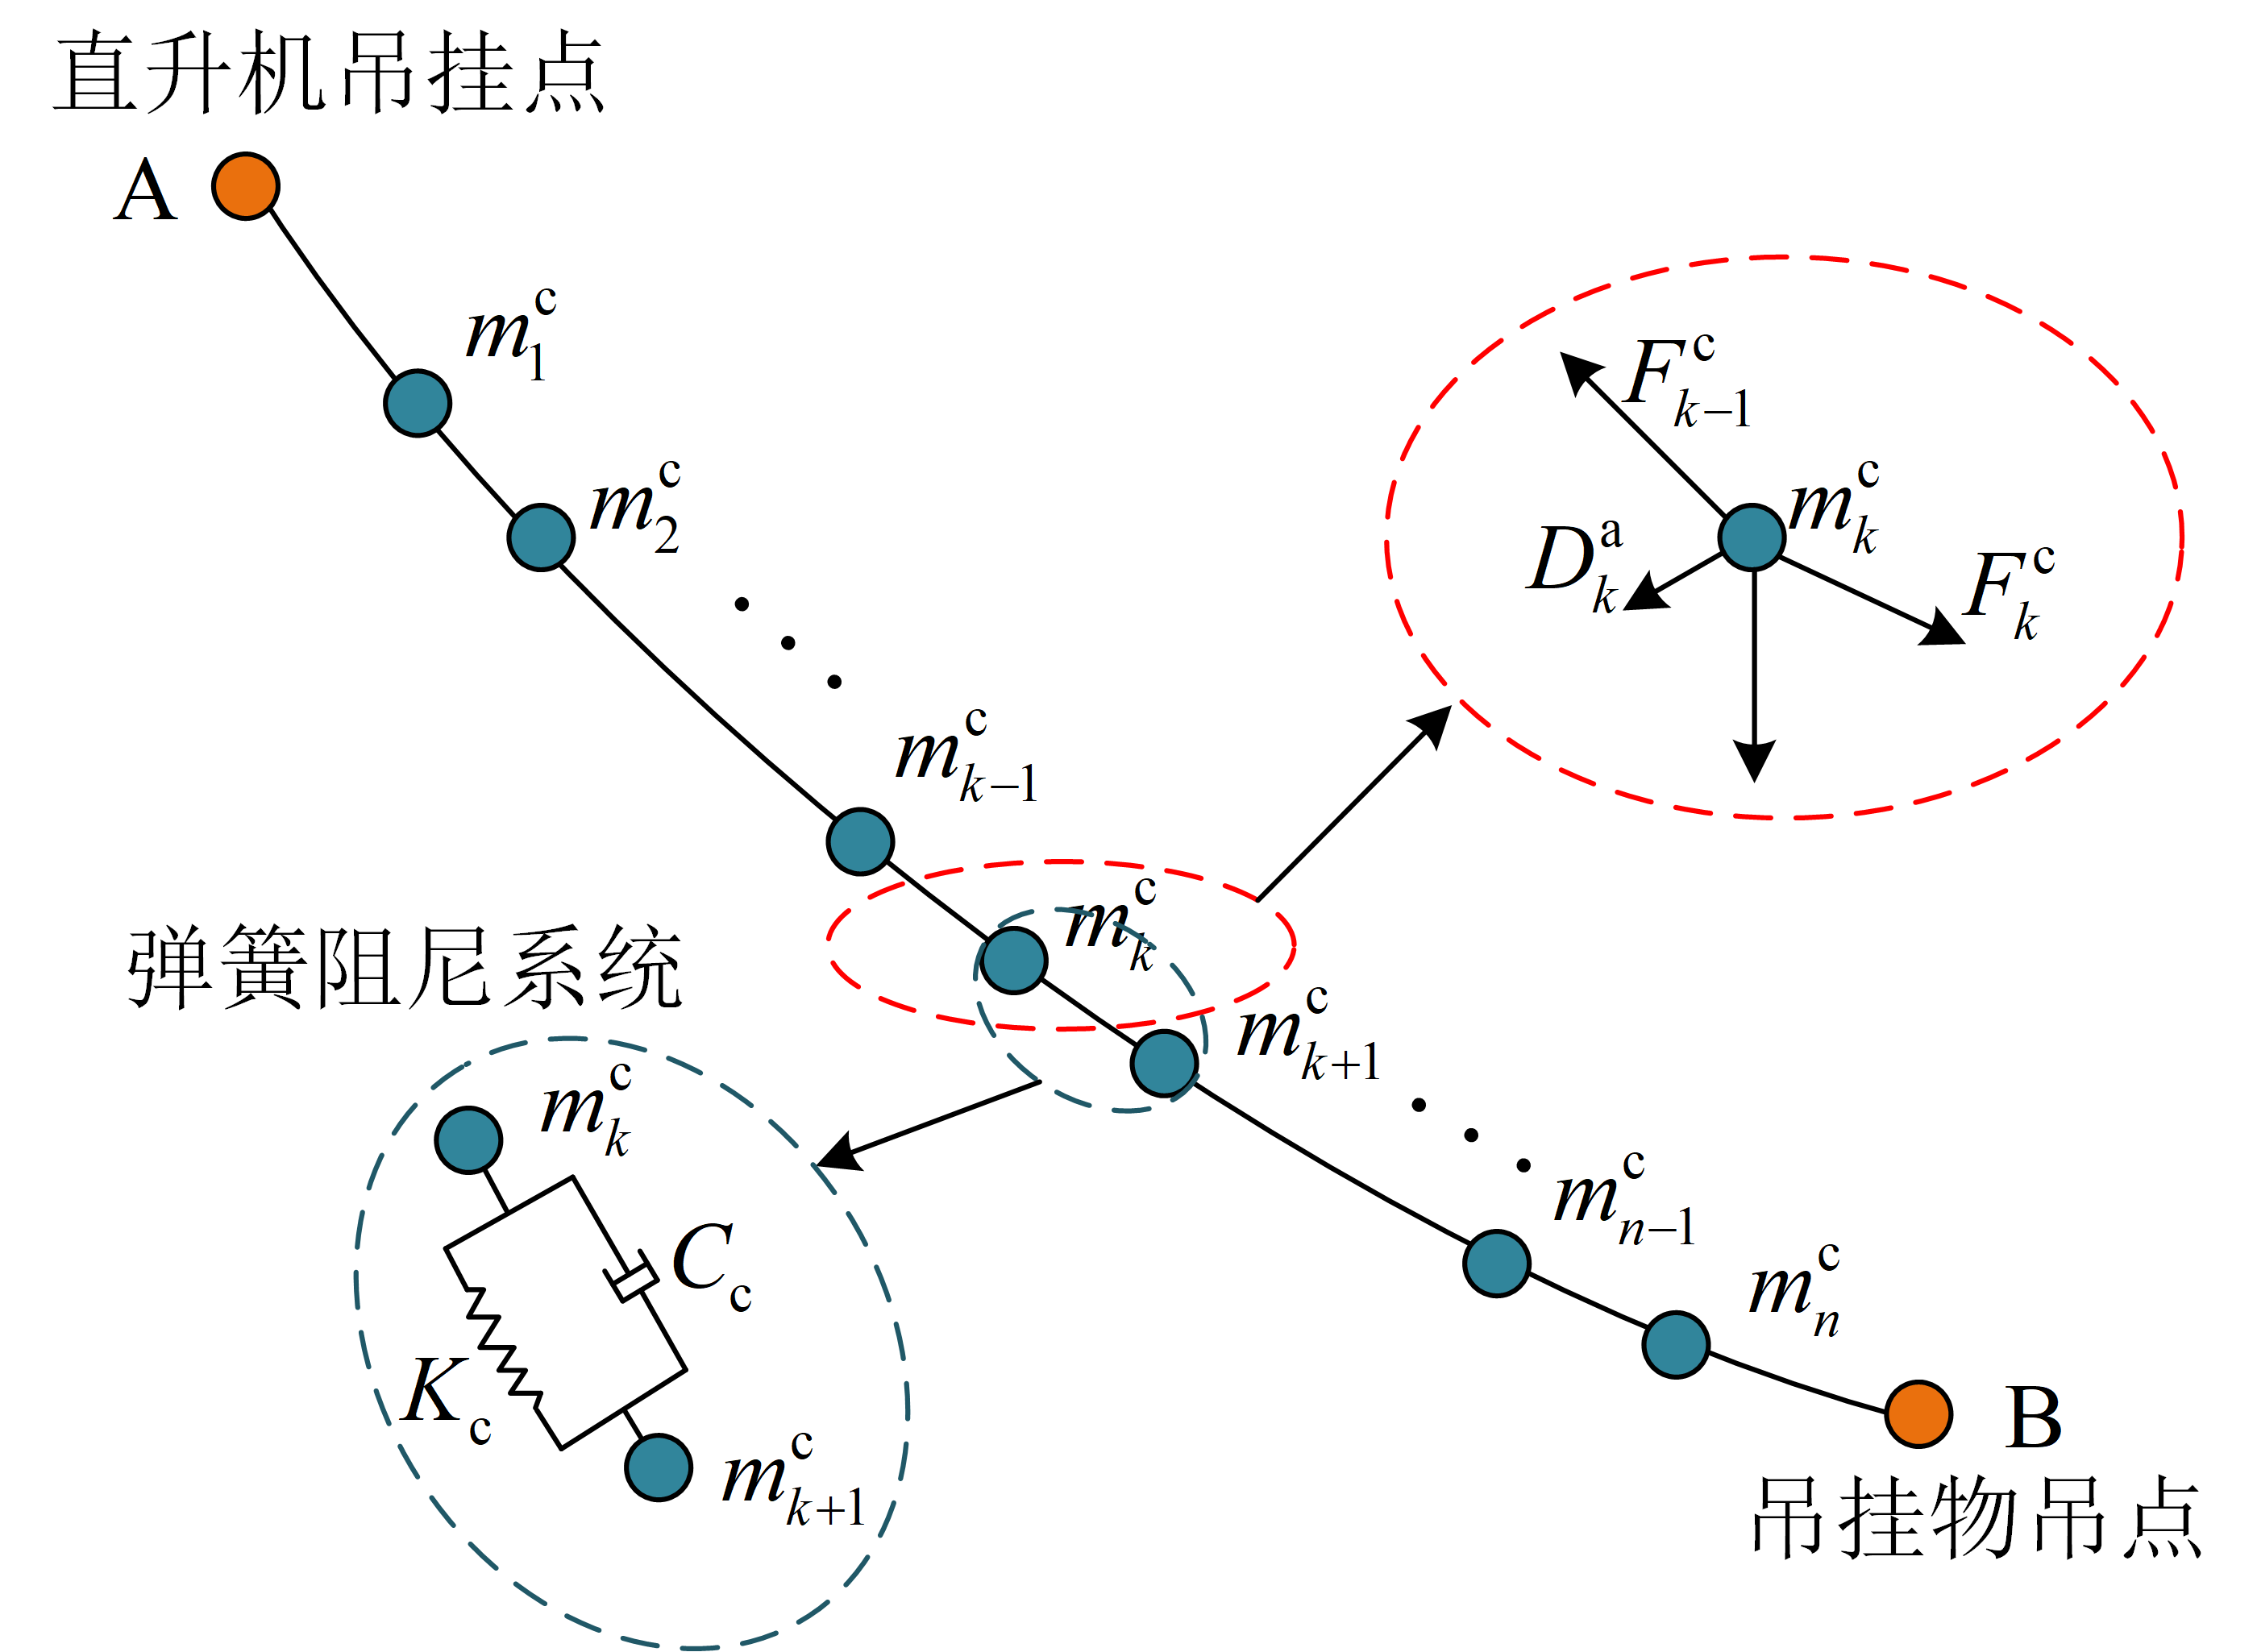
\includegraphics[width=8cm]{fig/figure_chap2/chap_2_4_2_1.png}
  \caption{吊索拉力、吊索角度定义}
  \label{fig:chap_2_4_2_1}
\end{figure}

\section{吊挂物模型}
假设吊挂物体轴系$x_Ly_Lz_L$原点位于吊挂物重心处,则基于牛顿-欧拉方法,吊挂物的动力学方程可以写为
\begin{equation}
  {{\bf{M}}_{\bf{L}}}{\dot{\bf{x}}} + {{\bf{C}}_{\bf{L}}}{\bf{x}} = {{\bf{g}}_L} + {{\bf{M}}_c} + {{\bf{M}}_{aero}}
  \label{equation:chap_4_1}
\end{equation}
其中,$\mathbf{M}_{aero}$是气动力、力矩,$\mathbf{M}_{c}$是由吊索引起的力和力矩,此外
\begin{equation}
  \left\{ {\begin{array}{*{20}{c}}
      {{{\bf{M}}_L} = \left[ {\begin{array}{*{20}{c}}
      {{{\bf{I}}_{3 \times 3}}}&{}&{}&{}\\
      {}&{{{\bf{I}}_{3 \times 3}}}&{}&{}\\
      {}&{}&{{m_L}{{\bf{I}}_{3 \times 3}}}&{}\\
      {}&{}&{}&{{{\bf{J}}_L}}
      \end{array}} \right]}\\
      {{{\bf{C}}_L}{\bf{x}} = \left[ {\begin{array}{*{20}{c}}
      {^e{{\bf{R}}_L}{\bf{V}}}\\
      {^{Euler}{{\bf{R}}_{Body}}{\bm{\omega }}}\\
      {{{\bf{0}}_{3 \times 3}}}\\
      {{\bm{\omega }} \times {{\bf{J}}_L}{\bm{\omega }}}
      \end{array}} \right]}\\
      {{g_L} = \left[ {\begin{array}{*{20}{c}}
      \begin{array}{l}
      \;\;\;\;\;\;\;\;\;{{\bf{0}}_{3 \times 1}}\\
      \;\;\;\;\;\;\;\;\;{{\bf{0}}_{3 \times 1}}\\
      ^L{{\bf{R}}_e}{\left[ {\begin{array}{*{20}{c}}
      0&0&{{m_L}g}
      \end{array}} \right]^T}
      \end{array}\\
      {{{\bf{0}}_{3 \times 1}}}
      \end{array}} \right]}\\
      {\dot{\bf{x}} = {{\left[ {\begin{array}{*{20}{c}}
      {^e{{\dot{\bf{P}}}_L}^T}&{\left[ {{{\dot \phi }_L},{{\dot \theta }_L},{{\dot \psi }_L}} \right]}&{\dot{\bf{V}}^T}&{{\bm{\dot \omega ^T}}}
      \end{array}} \right]}^T}\;}\\
      {{\bf{x}} = {{\left[ {\begin{array}{*{20}{c}}
      {^e{{\bf{P}}_L^T}}&{\left[ {{\phi _L},{\theta _L},{\psi _L}} \right]}&{\bf{V}^T}&{\bm{\omega ^T}}
      \end{array}} \right]}^T}}
      \end{array}} \right.
      \label{equation:chap_4_2_1}
\end{equation}
其中,$m_L$是吊挂物重量,$\mathbf{J}_L$是体轴系下的惯性矩阵,其对角元素为$J_{xx}$、$J_{yy}$、$J_{zz}$,$g$是重力加速度,$\mathbf{V}=[u_L,v_L,w_L]^T$和$\bm{\omega}=[p_L,q_L,r_L]^T$分别为$x_Ly_Lz_L$轴系下的线速度和角速度矢量,${^e{{\bf{P}}_L}}=[x_L,y_L,z_L]^T$是吊挂物在地轴系$x_ey_ez_e$的位置,$\left[ {{\phi _L},{\theta _L},{\psi _L}} \right]$是轴系${x_e}{y_e}{z_e}$和${x_L}{y_L}{z_L}$间的欧拉角,${{\bf{0}}_{m \times n}}$是$m$行$n$列的零矩阵,${{\bf{I}}_{m \times m}}$是$m$维单位矩阵,$^L{{\bf{R}}_e}$是轴系${x_e}{y_e}{z_e}$到${x_L}{y_L}{z_L}$的转换矩阵,$^e{{\bf{R}}_L}$是$^L{{\bf{R}}_e}$的转置,$^{Euler}{{\bf{R}}_{Body}}$是体轴系${x_L}{y_L}{z_L}$下的角速度到欧拉角速度的转换矩阵。

此外,可以发现,0.4$\times$0.4$\times$1 m的长方体吊挂物与标准8$\times$8$\times$20 ft MILVAN集装箱形状相似。采用6.1的长度比例因子,可以根据标准集装箱的风洞试验数据\cite{cicolani1987comprehensive,da2003unsteady,cicolani2009flight}得到本文研究的吊挂物的气动参数。

综上所述,式\ref{equation:chap_4_2_1}中的唯一未知量是由吊索引起的合力、合力矩$M_c$。换句话说,如果吊挂物轨迹和状态已知,通过式\ref{equation:chap_4_2_1}可以求出$\mathbf{M}_c$。


\section{基于涡方法的气动干扰计算}
\subsection{黏性涡粒子}
基于Lagrangian体系的粘性涡粒子方法(Viscous Vortex Particle Method, VVPM)可以模拟旋翼尾迹流场的演化过程,能较好捕捉旋翼复杂流场特性。VVPM的离散涡度场可以表示为:

\begin{equation}
    {\vec \omega ^h}\left( {\vec r,t} \right) = \sum\limits_{p = 1}^{{N_p}} {{{\vec \alpha }_p}\left( t \right)} \;\varsigma \left( {\vec r - {{\vec r}_p}\left( t \right);{R_p}} \right)
\end{equation}
其中,${\vec r_p}\left( t \right)$,${\vec \alpha _p}\left( t \right)$和${R_p}$分别为涡粒子$p$的空间位置、涡度和半径。$\varsigma \left( r \right)$是考虑每个粒子感应影响引起的涡度分布的截止函数。

涡量场可以基于Navier-Stokes方程描述,如下
\begin{equation}
    \frac{{D\vec \omega }}{{Dt}} = \vec \omega  \cdot \nabla \vec u + v{\nabla ^2}\vec \omega 
\end{equation}
其中,$\vec \omega  = \nabla  \times \vec u$是涡量场,$D\left( {} \right)/dt = \partial \left( {} \right)/\partial  + \vec u \cdot \left( {} \right)$是物质导数,${\nabla ^2} = {\partial ^2}/\partial {x^2} + {\partial ^2}/\partial {y^2} + {\partial ^2}/\partial {z^2}$是Laplacian算子。通过求解下列耦合的方程组,可以得到粒子涡度和位置的控制方程。
\begin{equation}
    \left\{ \begin{array}{l}
        \frac{{d{{\vec r}_p}}}{{dt}} = \vec u\left( {{{\vec r}_p}\left( t \right),t} \right)\\
        \frac{{d{{\vec \alpha }_p}}}{{dt}} = {{\vec \alpha }_p} \cdot \nabla \vec u\left( {{{\vec r}_p}\left( t \right),t} \right) + v\left[ {{\nabla ^2}{{\vec \alpha }_p}} \right]
        \end{array} \right.
    \label{equation:chap_2_5_1_1}
\end{equation}
其中,上述耦合方程组第一项代表涡量的输运效应,第二项表示涡量的耗散和拉伸效应。涡粒子的当地速度$\vec u\left( {\vec r,t} \right) = {\vec u_\infty }\left( {\vec r,t} \right) + {\vec u_i}\left( {\vec r,t} \right)$是自由流速度和诱导速度的和。诱导速度可以通过Biot-Savart理论求得,如下
\begin{equation}
    {\vec u_i}\left( {\vec r,t} \right) = \int_{{V_0}} {\vec K\left( {\vec r,{{\vec r}_0}} \right)}  \times \vec \omega \left( {{{\vec r}_0},t} \right)d{V_0}
\end{equation}
其中,$\vec K\left( {\vec r,{{\vec r}_0}} \right) = G\left( {\vec r,{{\vec r}_0}} \right) - \varsigma \left( {\vec r,{{\vec r}_0}} \right)$是Biot-Savart核函数,$G\left( {\vec r,{{\vec r}_0}} \right)$是Green函数的矢量形式。通过将涡粒子场的控制方程组代入上述方程,诱导速度可以重新写成
\begin{equation}
    \vec u_i^h\left( {\vec r,t} \right) = \sum\limits_{p = 1}^{{N_p}} {{{\vec K}^h}\left( {\vec r - {{\vec r}_p}\left( t \right)} \right) \times {{\vec \alpha }_p}\left( t \right)} 
\end{equation}

核函数的表达式应该与截止函数$\varsigma \left( {\vec r} \right)$的表达式相对应。本文中,采用Dirac delta截止函数,Rosenhead-Moore核函数。其中,核函数的表达式如下
\begin{equation}
    {\vec K^h}\left( {\vec x,\vec y} \right) =  - \frac{1}{{4\pi }}\frac{{\vec x - \vec y}}{{{{\left( {{{\left| {\vec x - \vec y} \right|}^2} + R_v^2} \right)}^{3/2}}}}
\end{equation}

此外,式\ref{equation:chap_2_5_1_1}中,$v\left[ {{\nabla ^2}{{\vec a}_p}} \right]$表示涡量输运过程中由于空气黏性影响导致的黏性输运效应。本文通过Particle Strength Exchange (PSE)方法求解。PSE方法的关键是用积分算子代替Laplacian算子${\nabla ^2}$,以避免直接的数值积分。基于PSE方法,黏性输运项可以重写为
\begin{equation}
    \frac{{d{{\vec \alpha }_p}}}{{dt}}\left| {_{PSE} = v\sum\limits_{j \in {P_i}} {\left( {{V_p}{{\vec \alpha }_p} - {V_j}{{\vec \alpha }_j}} \right)\varsigma \left( {{{\vec x}_p} - {{\vec x}_j};{R_j}} \right)} } \right.
\end{equation}

由于核函数会随着距离的增加而迅速衰减,因此只考虑靠近当前粒子的涡粒子,而忽略所有超过设定截断距离的粒子的影响。因此,计算中将只记及相邻粒子的影响。在本研究中,PSE方法的截止距离与下面讨论的加速算法的区域分割距离一致。

从上述涡粒子诱导速度计算中可以发现,在求解粒子对流速度项或速度梯度项时,需要考虑N个粒子的总贡献。这类似于经典的N体问题。对于这类问题,TreeCode[33]和快速多极算法(Fast Multipole Algorithm, FMM)[34]是两种常见的加速算法。这两种算法都需要生成相应的数据结构,这些数据结构通常是八叉树的形式。如果不采用加速算法,则N个粒子的直接数值解规模为$O\left( {{N^2}} \right)$。采用加速算法后,TreeCode的解规模为$O\left( {N\log N} \right)$,FMM算法的解规模为$O\left( N \right)$。显然,随着时间的推移,涡粒子的数量迅速增加,TreeCode和FMM算法的加速效果将越来越显著。

由于涉及多旋翼间的干扰,本研究中涡粒子数量较多。为了尽可能提高计算效率,采用FMM算法作为加速技术。在FMM算法中,如果两个涡元区域(一组分割的涡流粒子)之间的间隔大于设定的截断距离,则源区域对目标区域的影响首先扩展为多极序列。在目标区域,将多极级数转化为局部泰勒展开,从而快速获得该区域内所有涡旋粒子的诱导速度。FMM算法用于计算涡旋粒子的诱导速度、速度梯度和粘性扩散效应。
\subsection{升力面/涡格法}
旋翼桨叶气动模型包括旋翼拉力、桨叶挥舞和诱导速度的计算。之前的研究中广泛使用了升力线[35]和升力面[36]的方法。相比之下,后者具有更高的计算精度,可以分析更复杂的叶片三维形状(如尖削和后掠)。基于这一考虑,采用升力面/涡格法作为叶片气动模型。

在研究中,首先将整个叶片沿展向分为几个微段,然后用无厚度的中间弧面来表示。对于后掠和尖削叶片,应修改叶片前后边缘的相应网格线,网格分区应与叶片段相对应。图\ref{fig:chap2_5_2_1}是一种典型情况,叶片的升力面网格分为S1和S2段,其中前者为直线段,后者为后掠段。

\begin{figure}[!htb]
    \centering
    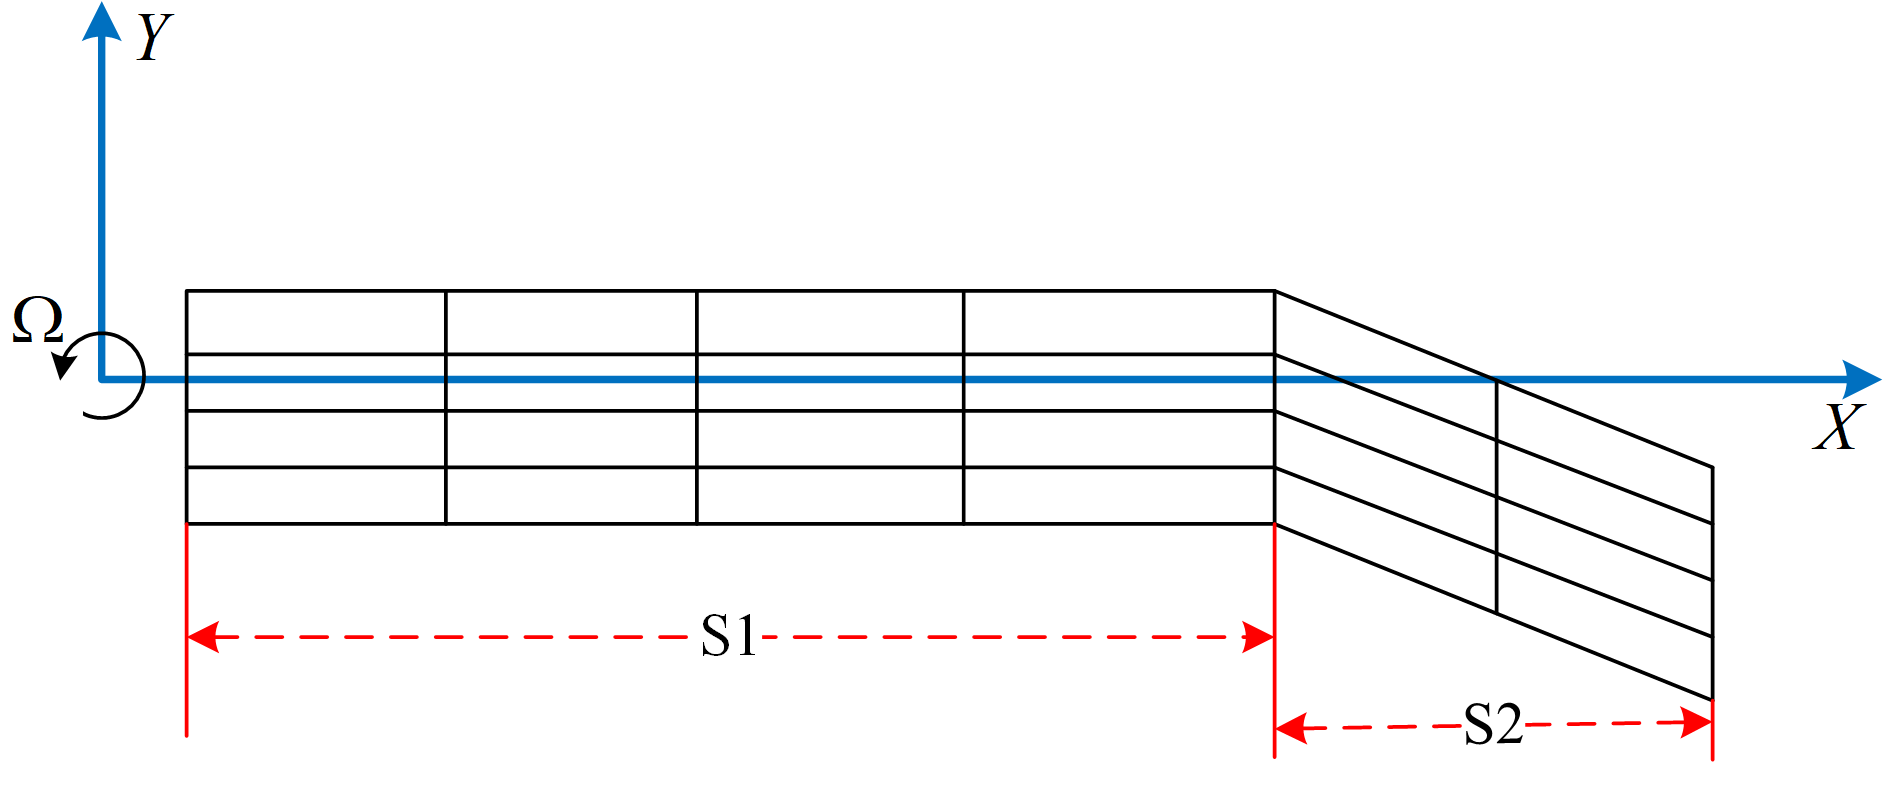
\includegraphics[width=7cm]{fig/figure_chap2/chap_2_5_2_1.png}
    \caption{带后掠的桨叶涡面网格划分}
    \label{fig:chap2_5_2_1}
  \end{figure}

将叶片沿展向分为几列,沿弦向分为几行,那么叶片表面将被划分为若干网格。虽然每个叶片段的展向编号不同,但弦向编号应保持不变。叶片的中弧面由涡四边形代替,涡四边形的展向附涡位于网格的四分之一弦线上,弦向附涡沿展向网格分布。在网格边界处,涡四边形的后缘涡位于相邻网格的四分之一弦线上。在叶片的后缘上,涡格等效地生成涡粒子团,如图\ref{fig:chap2_5_2_2}所示。

\begin{figure}[!htb]
    \centering
    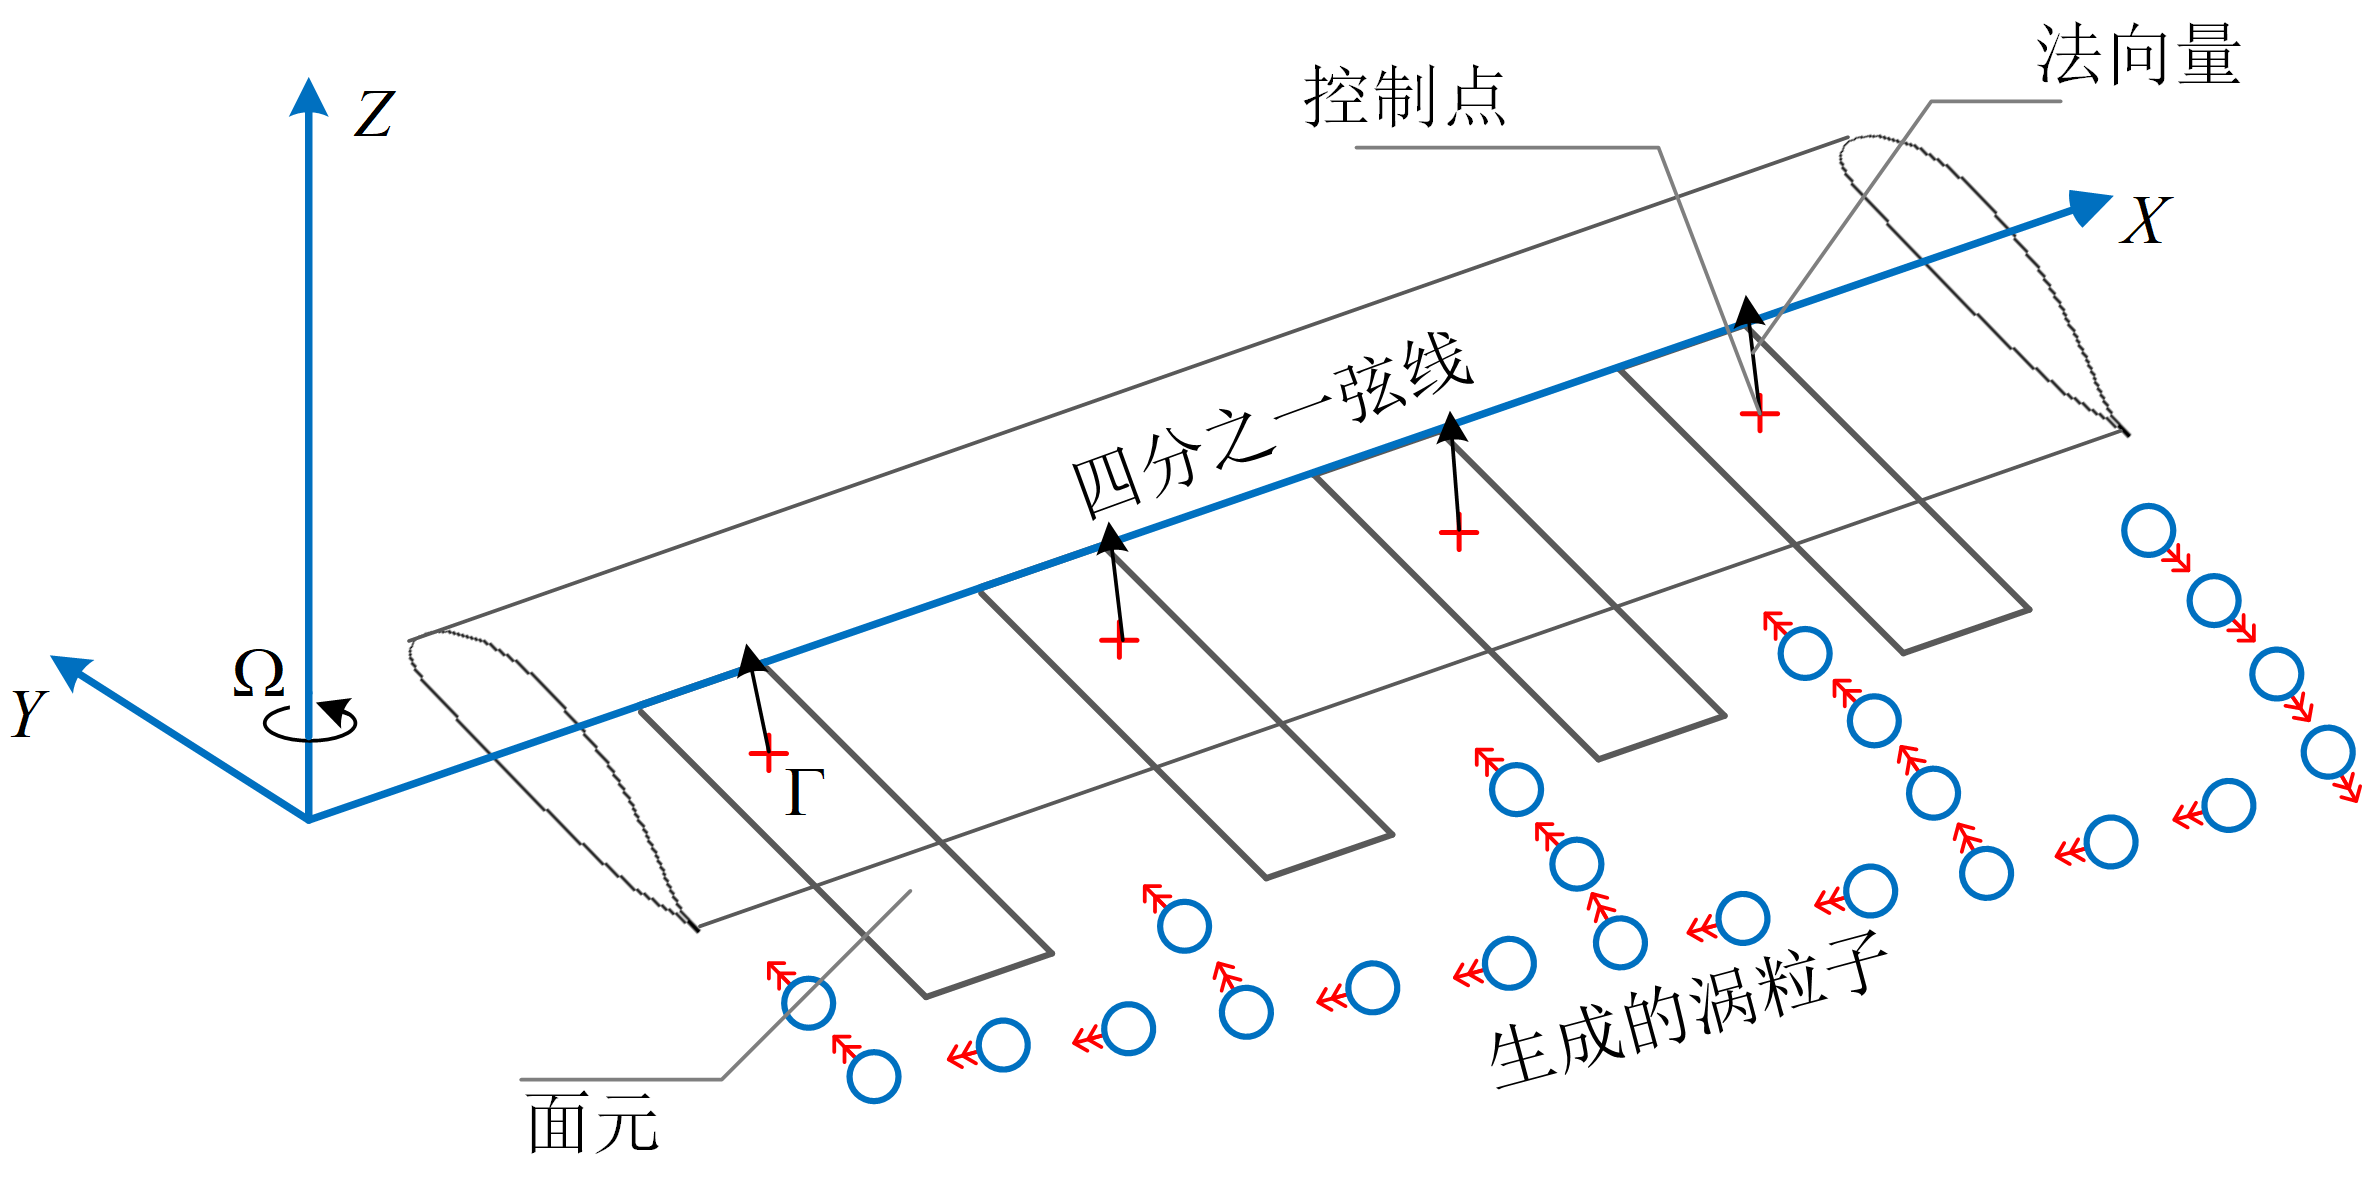
\includegraphics[width=7cm]{fig/figure_chap2/chap_2_5_2_2.png}
    \caption{桨叶上的涡元分布和后缘涡粒子生成示意图}
    \label{fig:chap2_5_2_2}
  \end{figure}

在每个叶片段后缘会产生涡源,并脱落到旋翼尾迹中。其中,涡源可以通过下式计算
\begin{equation}
    {r_{wake}} =  - \frac{{d{{\vec \Gamma }_b}}}{{dt}} + {\vec v_b}\nabla  \cdot {\vec \Gamma _b}
\end{equation}
其中,${r_{wake}}$为新产生的涡的强度。${\vec \Gamma _b}$是叶片约束环量的矢量形式。${\vec v_b}$是包含桨叶运动速度、远方来流速度、诱导速度、其他涡源干扰速度在内的当地合速度。在上面的公式中,第一项表示叶片约束环量的展向变化产生的尾涡,第二项表示叶片约束环量的方位变化产生的脱落涡。

\subsection{方法验证}
基于上述涡方法,对悬停状态下的Caradonna–Tung旋翼、前飞状态下的Scaled-model旋翼、以及纵列式双旋翼开展了分析。通过将计算结果与风洞试验数据进行对比,验证了本文建立的涡方法的有效性和可行性。

\begin{figure}[!htb]  
  \subfloat[$速度场$]{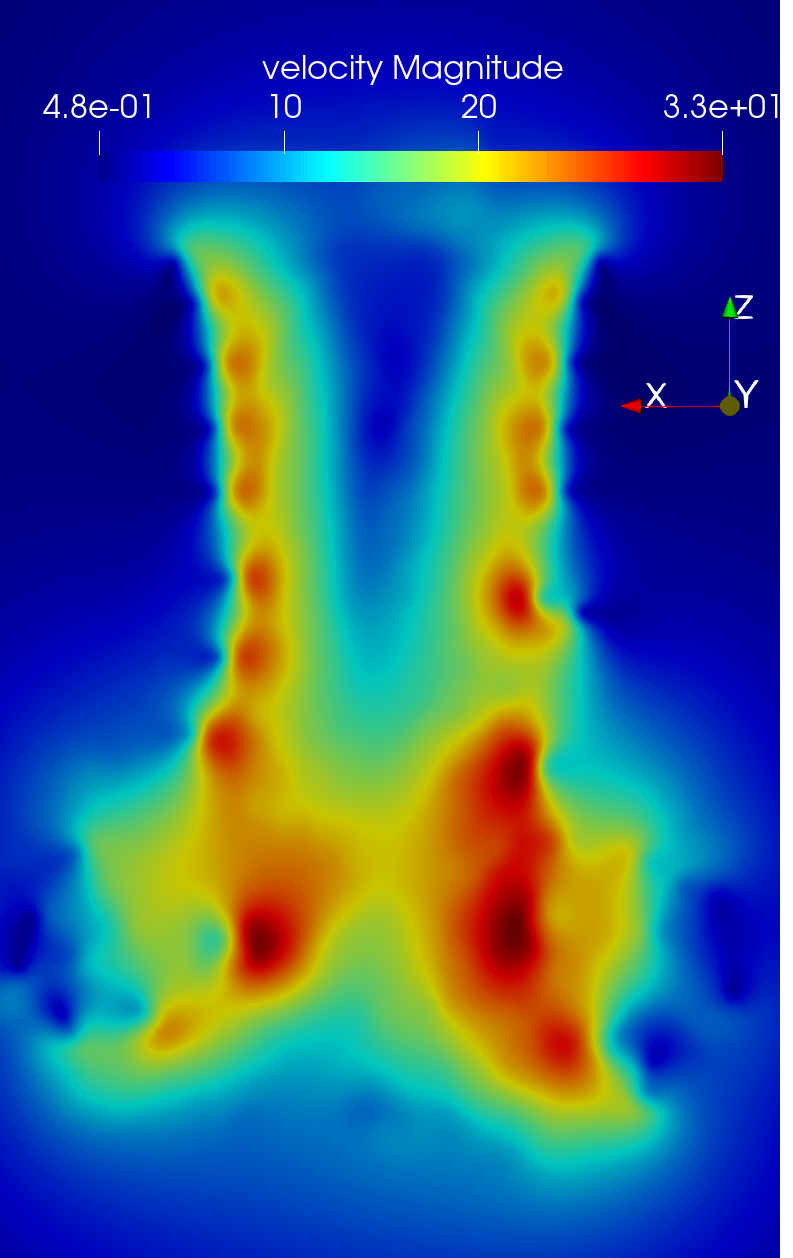
\includegraphics[width=4cm]{chap_2_5_3_1_1_1.png}}\quad
  \subfloat[$尾迹结构$]{\includegraphics[width=6cm]{chap_2_5_3_1_1_2.png}}\quad
  \subfloat[$涡度场$]{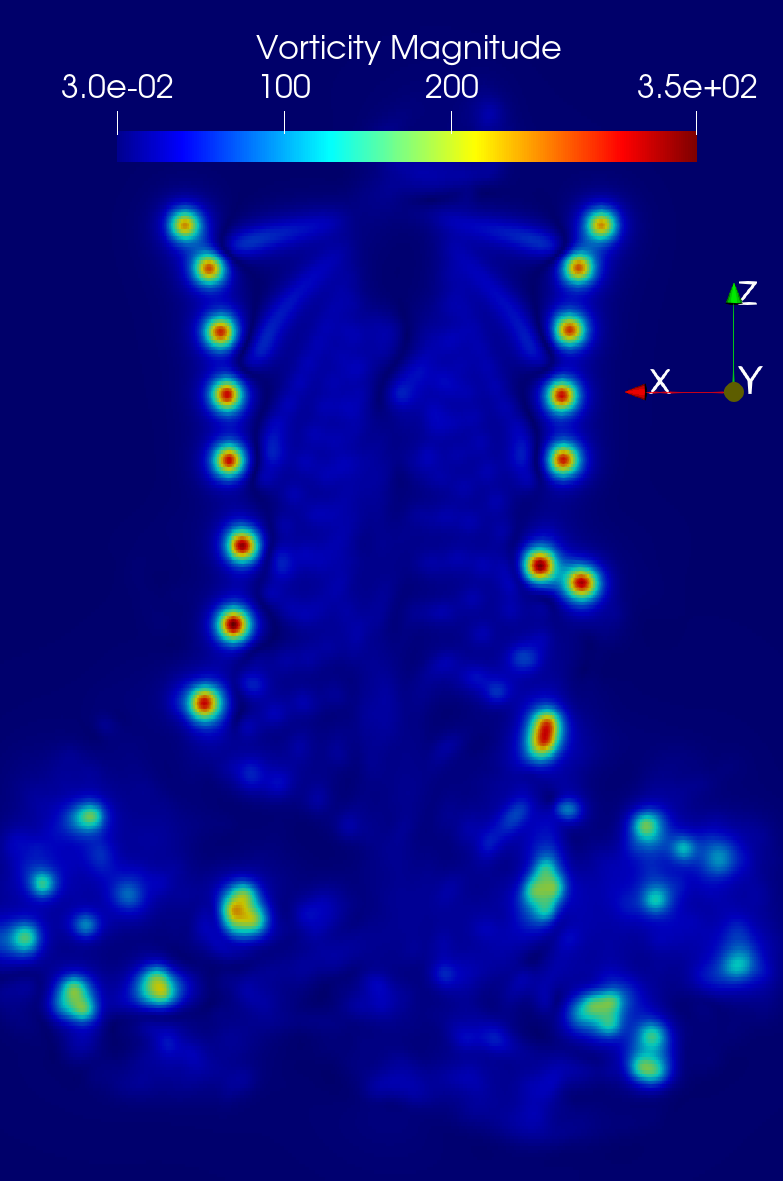
\includegraphics[width=4cm]{chap_2_5_3_1_1_3.png}}\quad\\
    \subfloat[$C_T$]{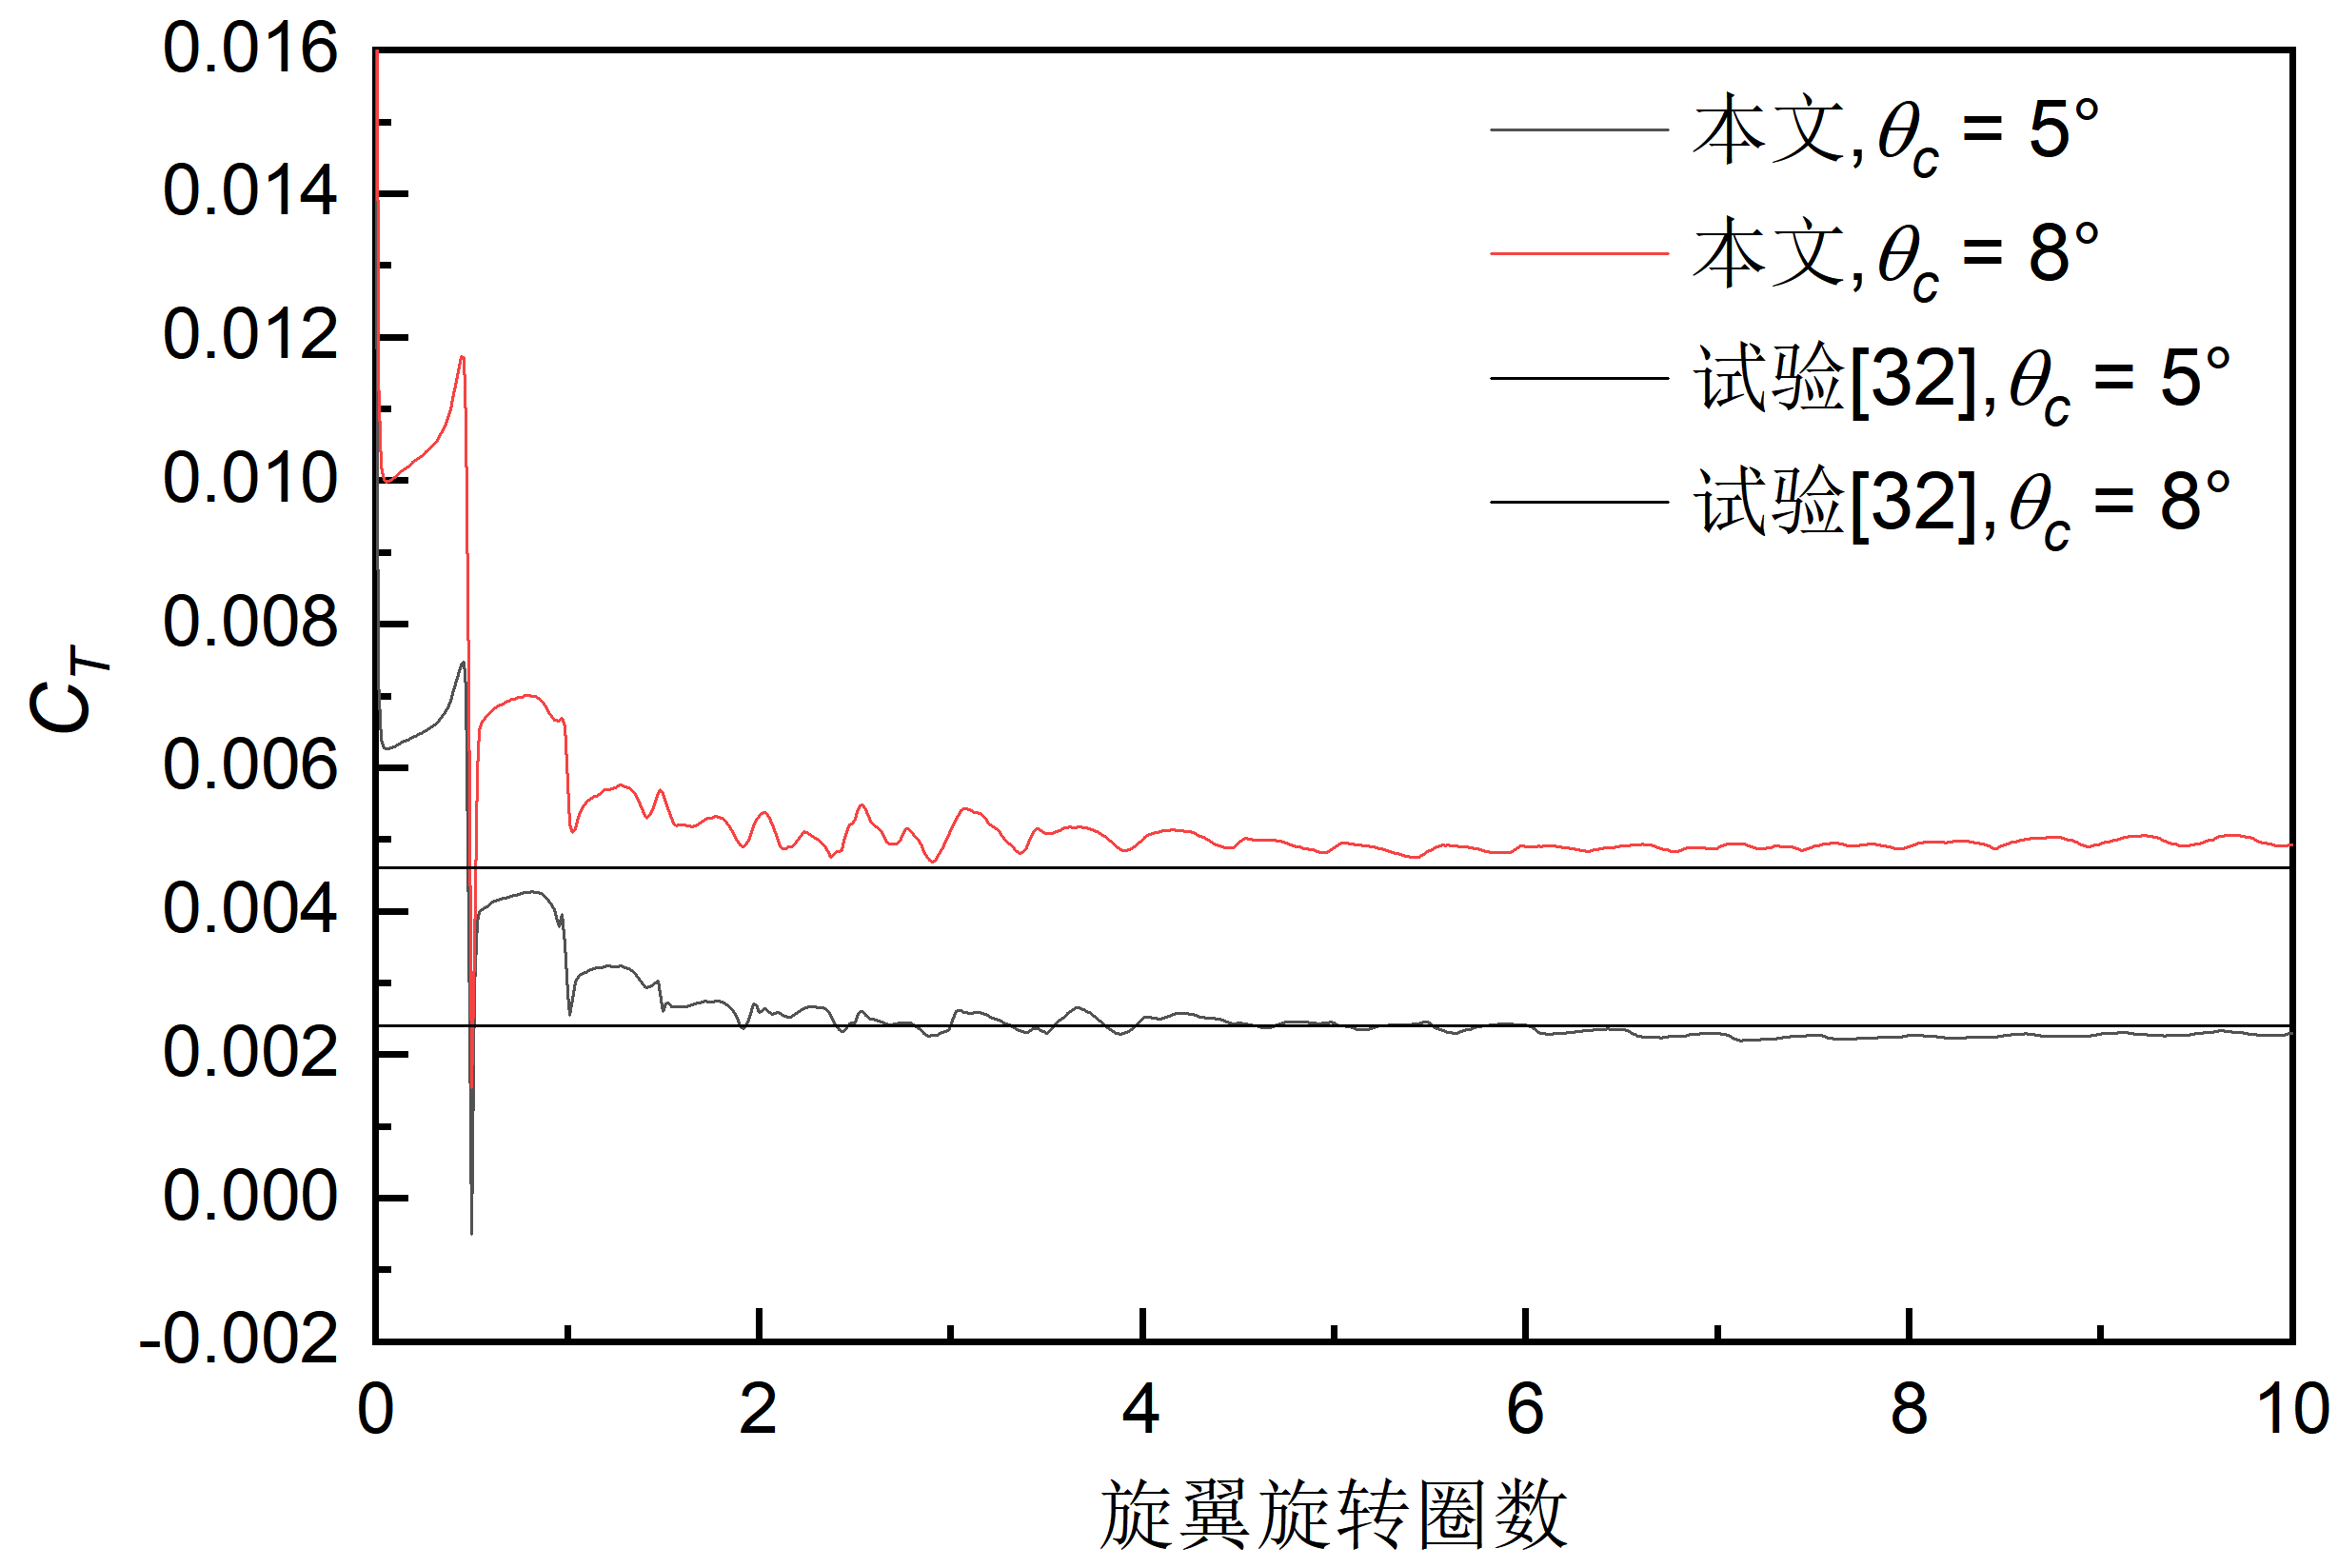
\includegraphics[width=7.3cm]{chap_2_5_3_1_2.png}}\quad
      \subfloat[升力系数]{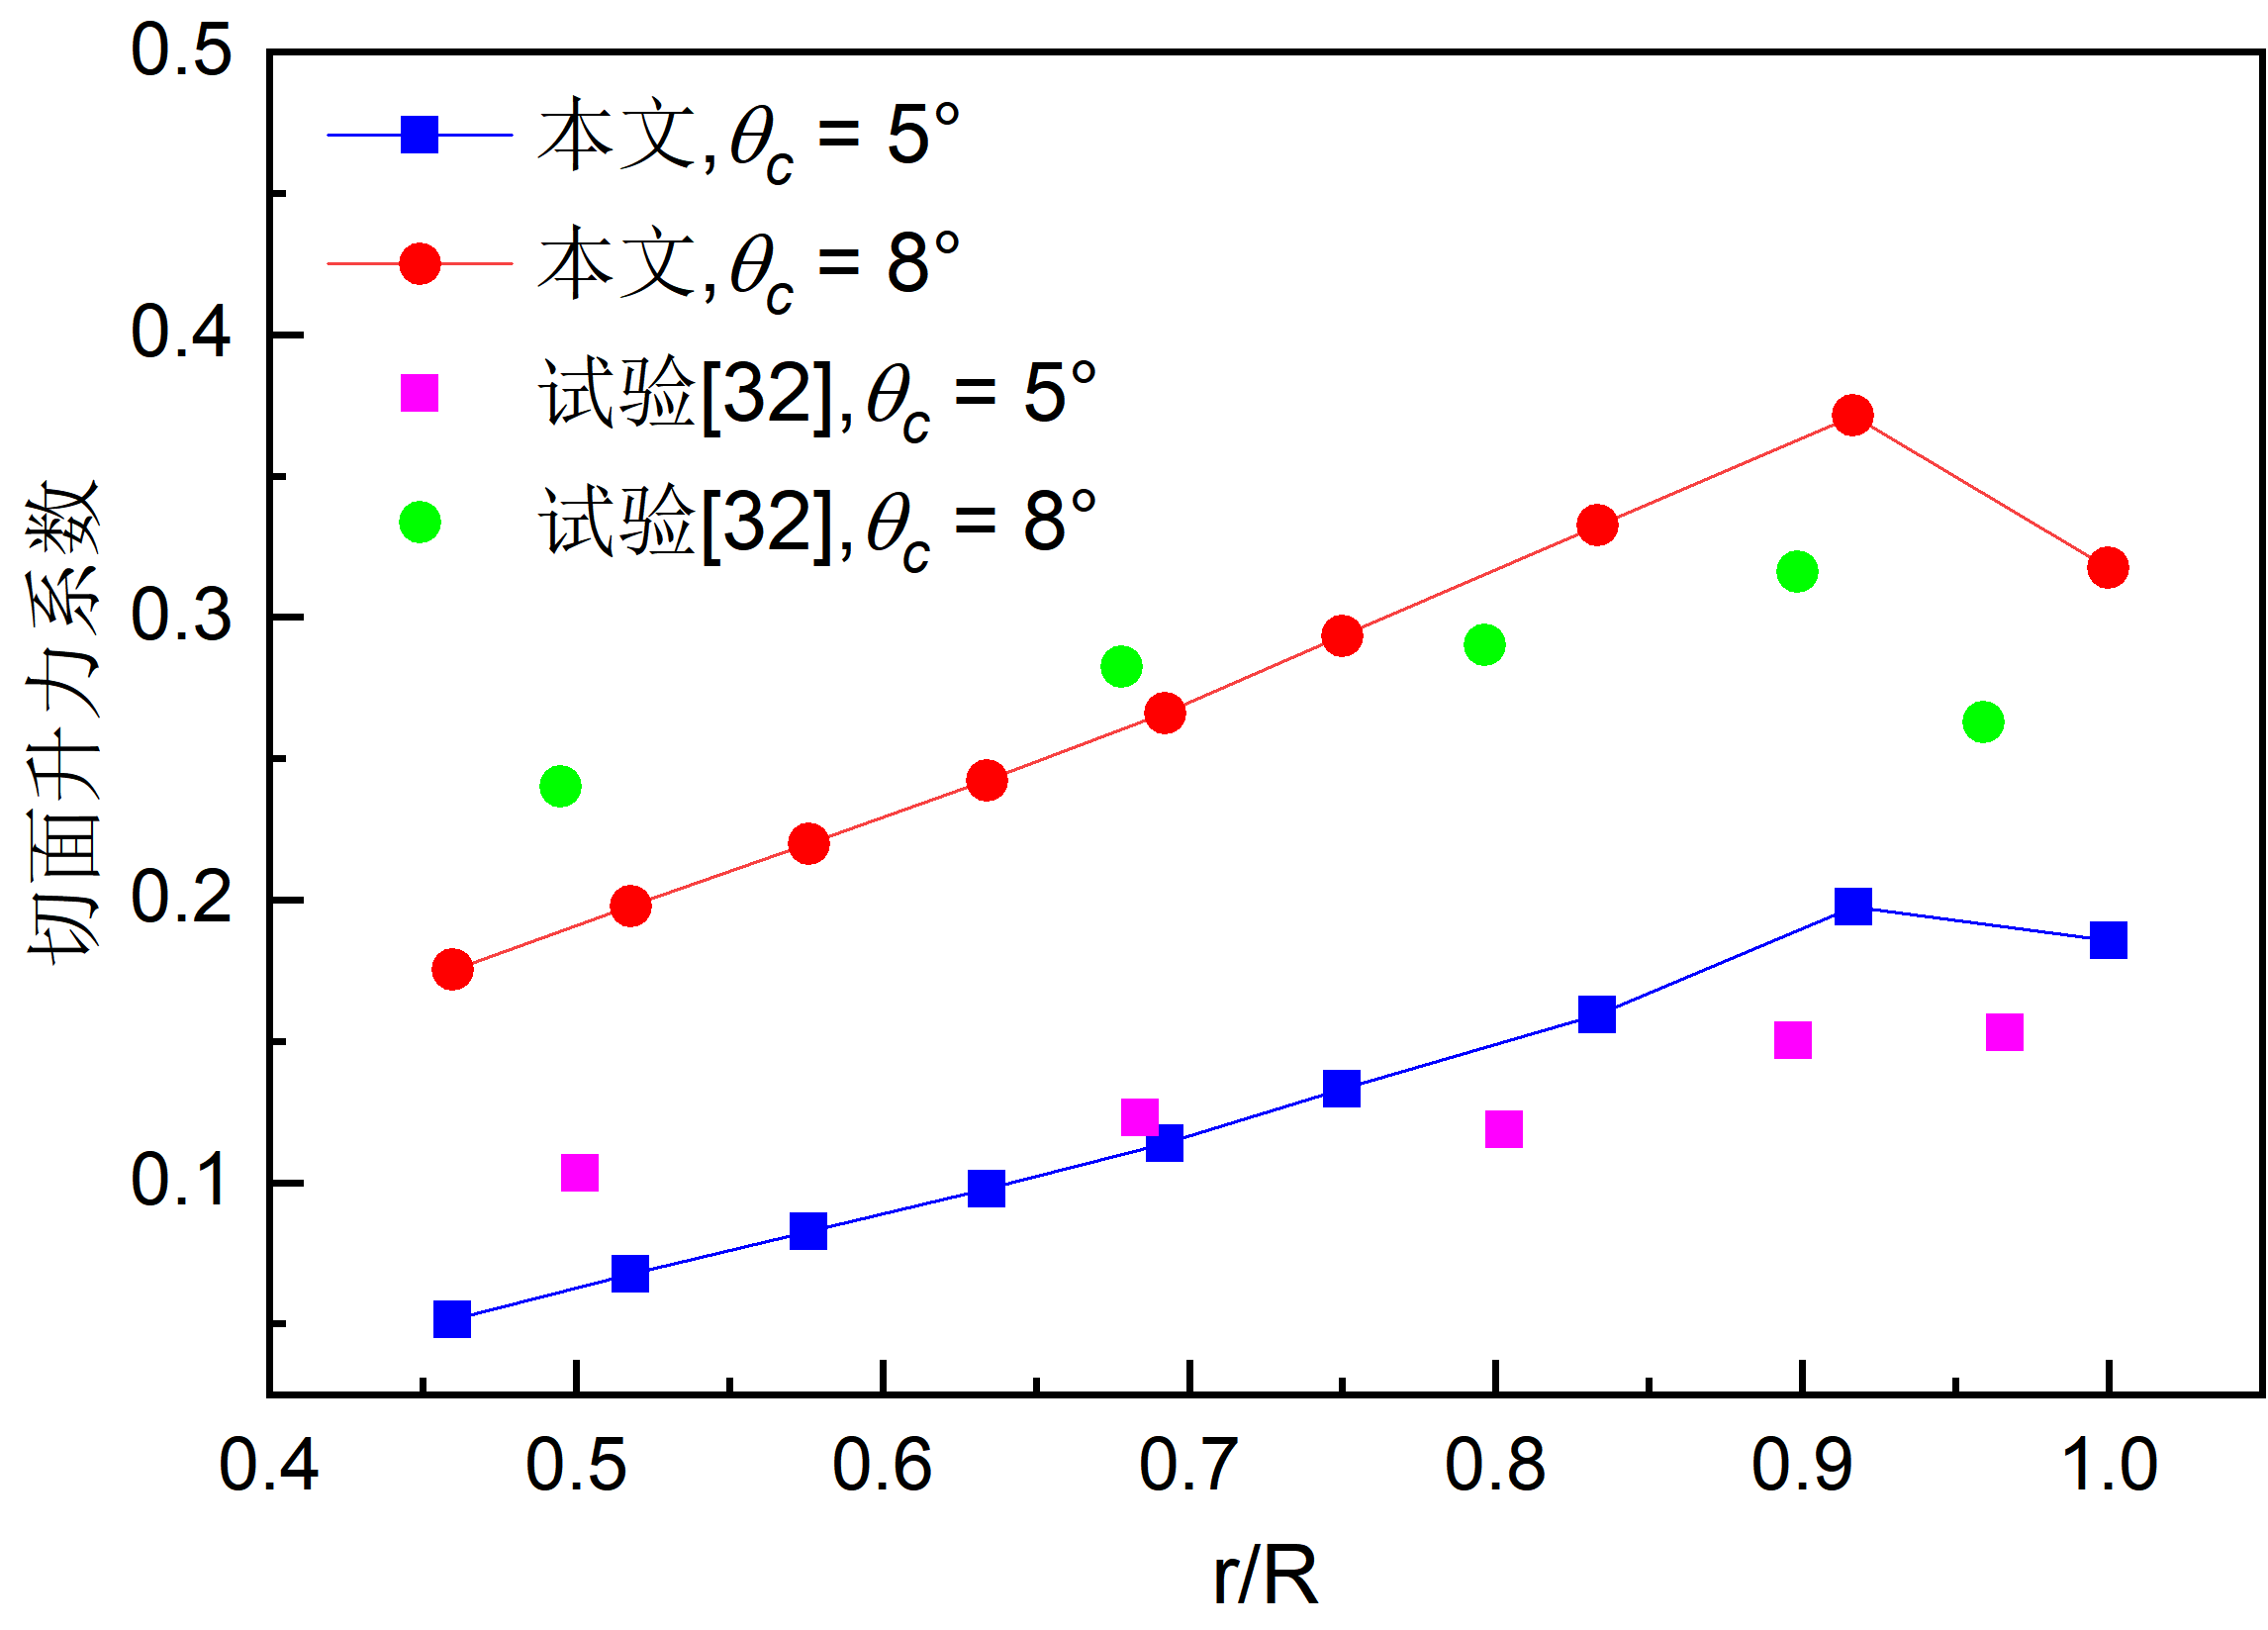
\includegraphics[width=7cm]{chap_2_5_3_1_3.png}}\\
      \caption{Caradonna–Tung旋翼计算结果与试验结果对比}
      \label{fig:chap2_5_3_1_2}
\end{figure}

\subsubsection{悬停状态下的Caradonna–Tung旋翼}
悬停状态下的Caradonna–Tung旋翼试验数据见参考文献\cite{caradonna1981experimental}。该旋翼有两片桨叶,桨叶翼型为NACA0012,无负扭、无尖削。旋翼半径为1.143 m,桨叶弦长为0.19 m,旋翼转速为1250 rpm。采取桨距为5 \degree 、8 \degree 时开展验证。

图\ref{fig:chap2_5_3_1_2}(a)-(c)给出了桨距为8 \degree 时旋翼旋转10圈后的速度场、尾迹结构、涡度场,可以清楚地捕捉到两片桨叶的桨尖涡和远场的管束区域,给出了尾迹的收缩、扩张、非周期、扩散、伸展运动。图\ref{fig:chap2_5_3_1_2}拉力系数的收敛过程。桨距为5 \degree 时,风洞试验拉力系数为0.0024;桨距为8 \degree 时,风洞试验拉力系数为0.0046。5个旋转周期后,计算值与试验值误差小于5 \%。图\ref{fig:chap2_5_3_1_2}给出了沿桨叶径向的载荷分布,基于涡方法计算得到的切面升力系数与试验值虽然有一定的差别,但整体趋势是一致的。

\begin{figure}[!htb]
  \centering
  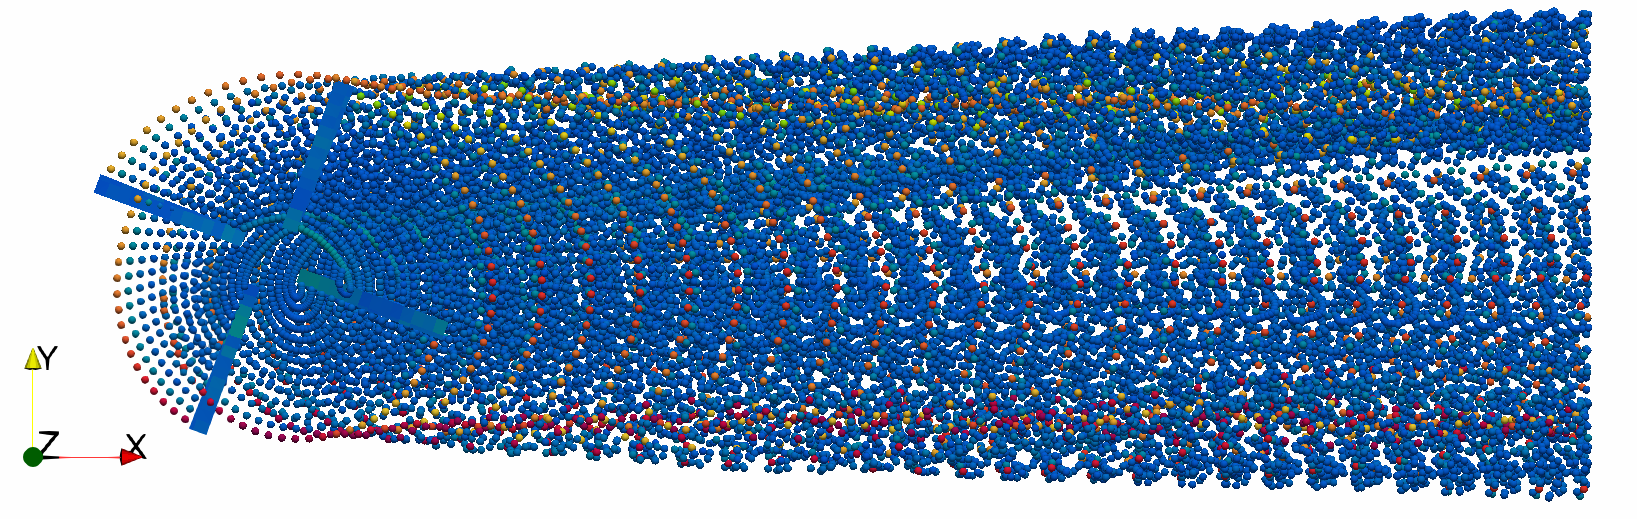
\includegraphics[width=10cm]{fig/figure_chap2/chap_2_5_3_2_1.png}
  \caption{前飞状态下的Scaled-model旋翼尾迹}
  \label{fig:chap2_5_3_2_1}
\end{figure}

\begin{figure}[!htb]  
  \subfloat[纵向入流速度]{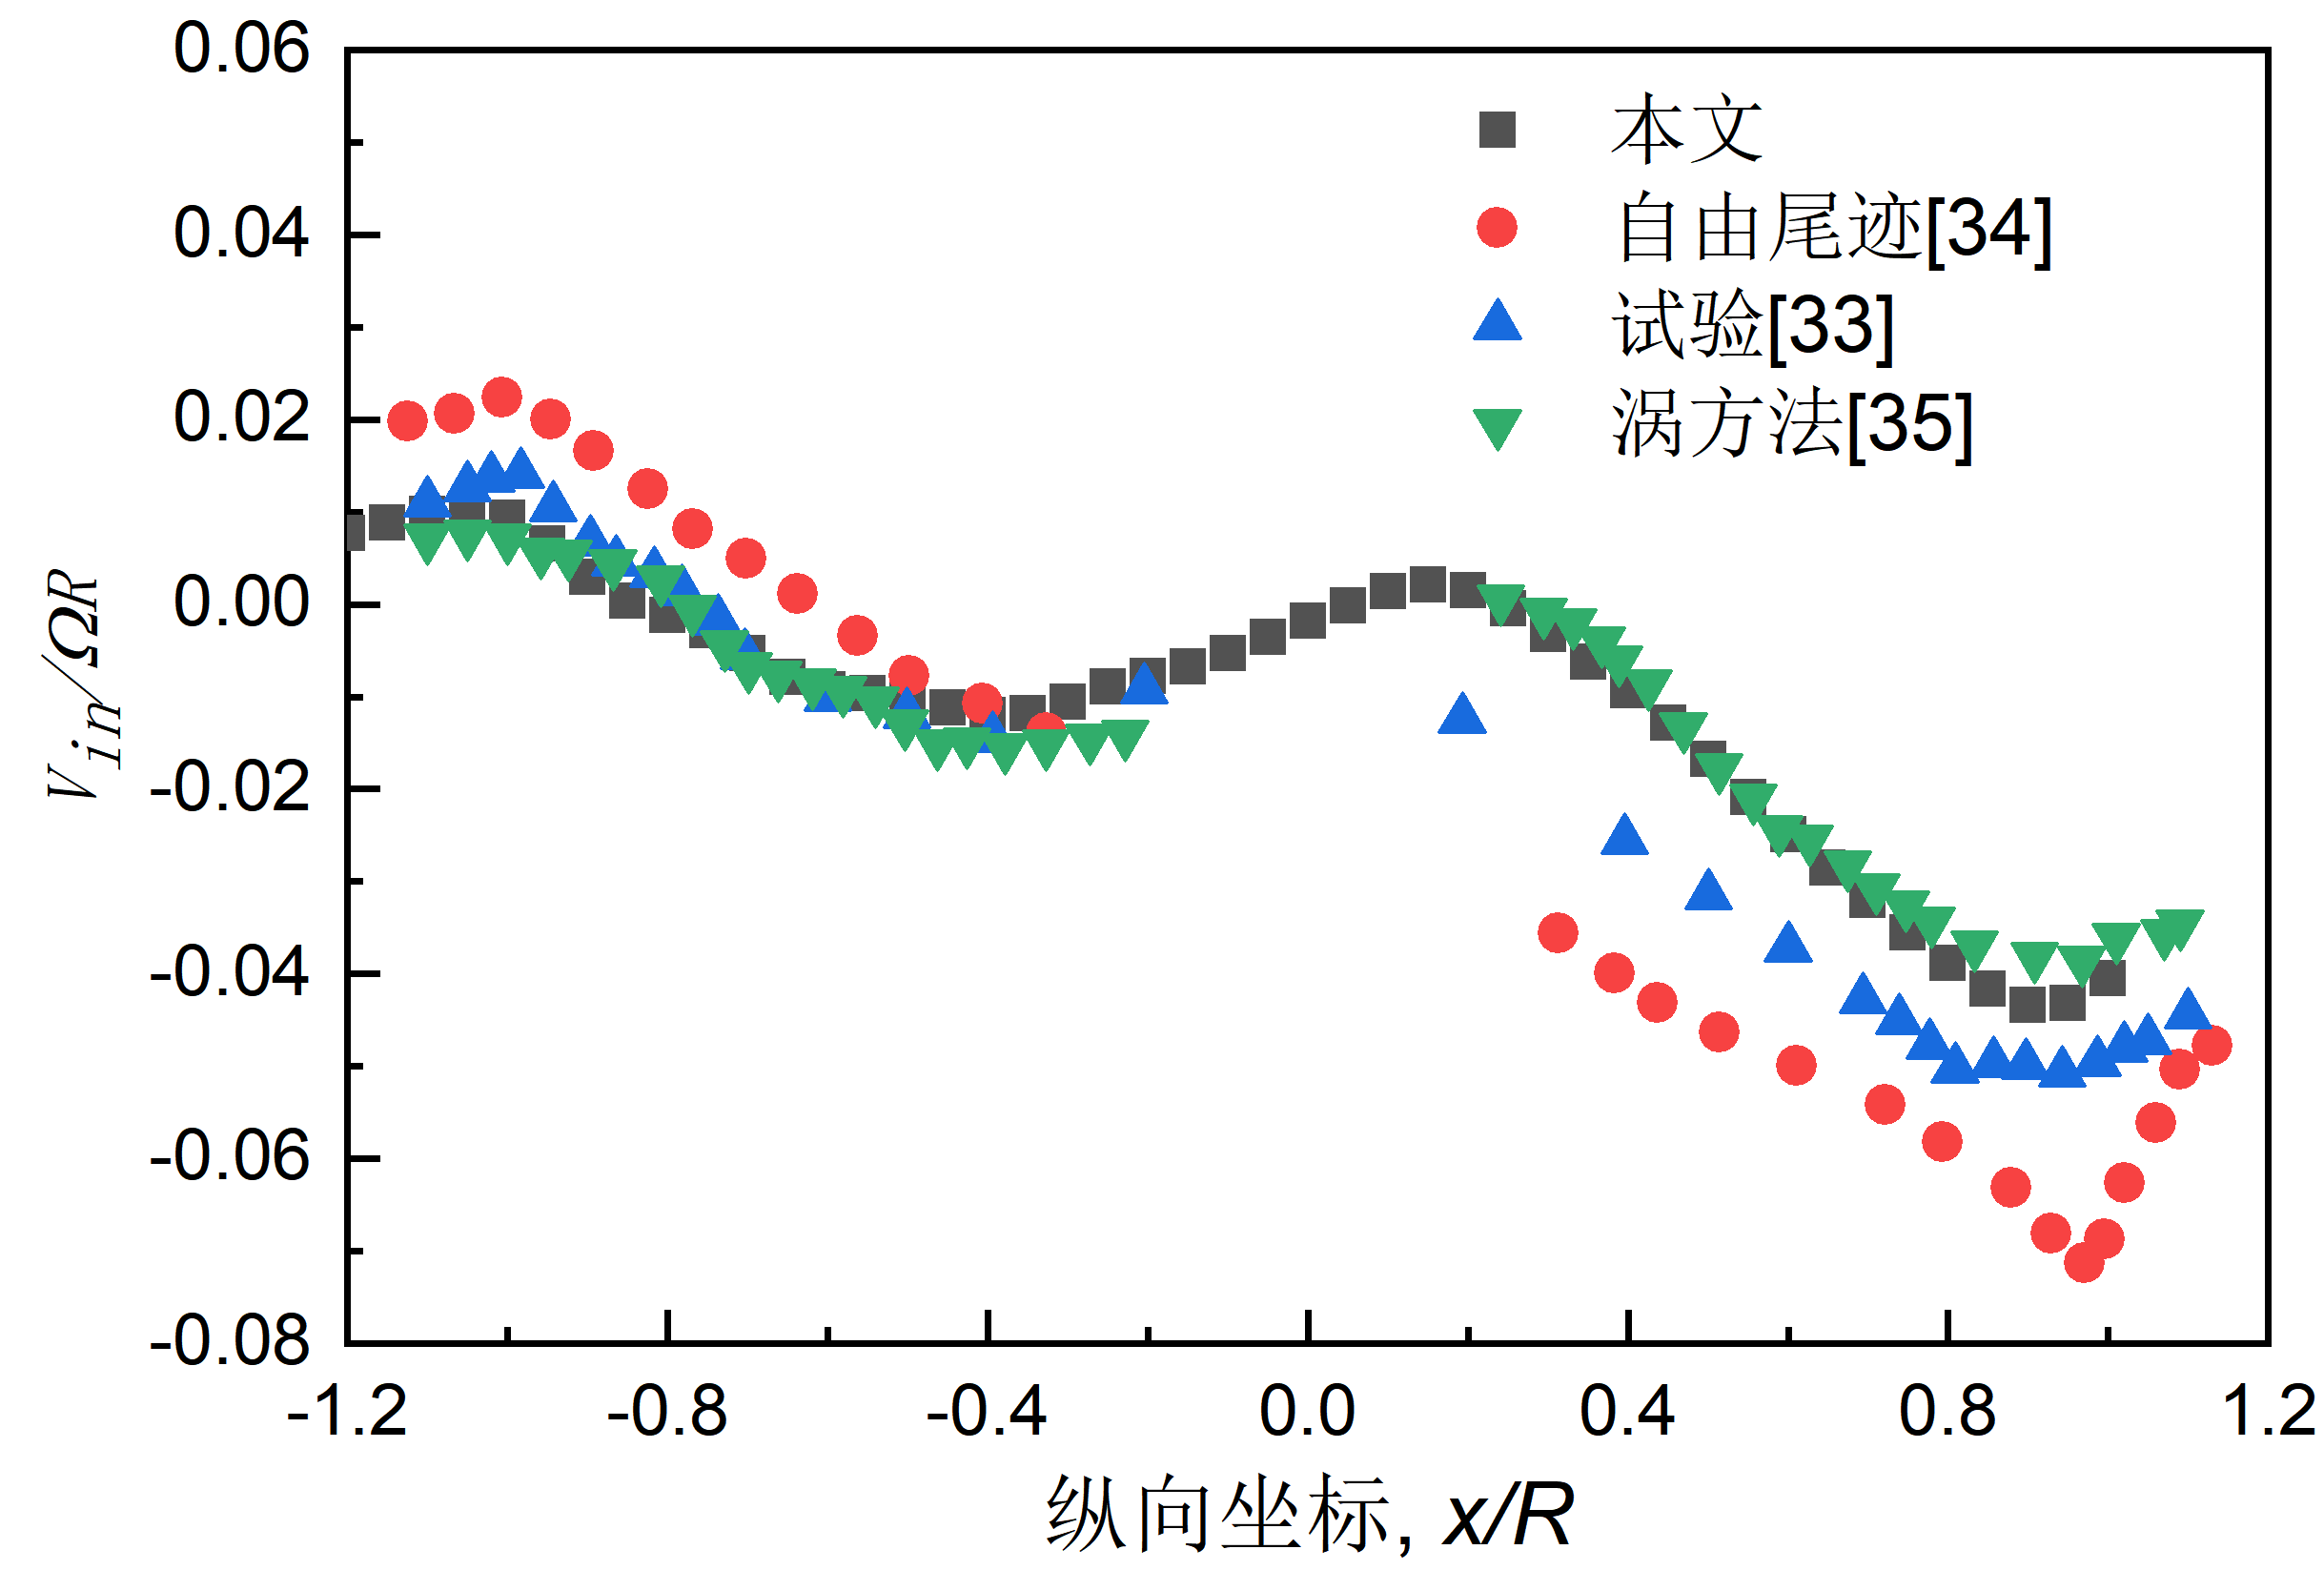
\includegraphics[width=7cm]{chap_2_5_3_2_2.png}}\quad
    \subfloat[横向入流速度]{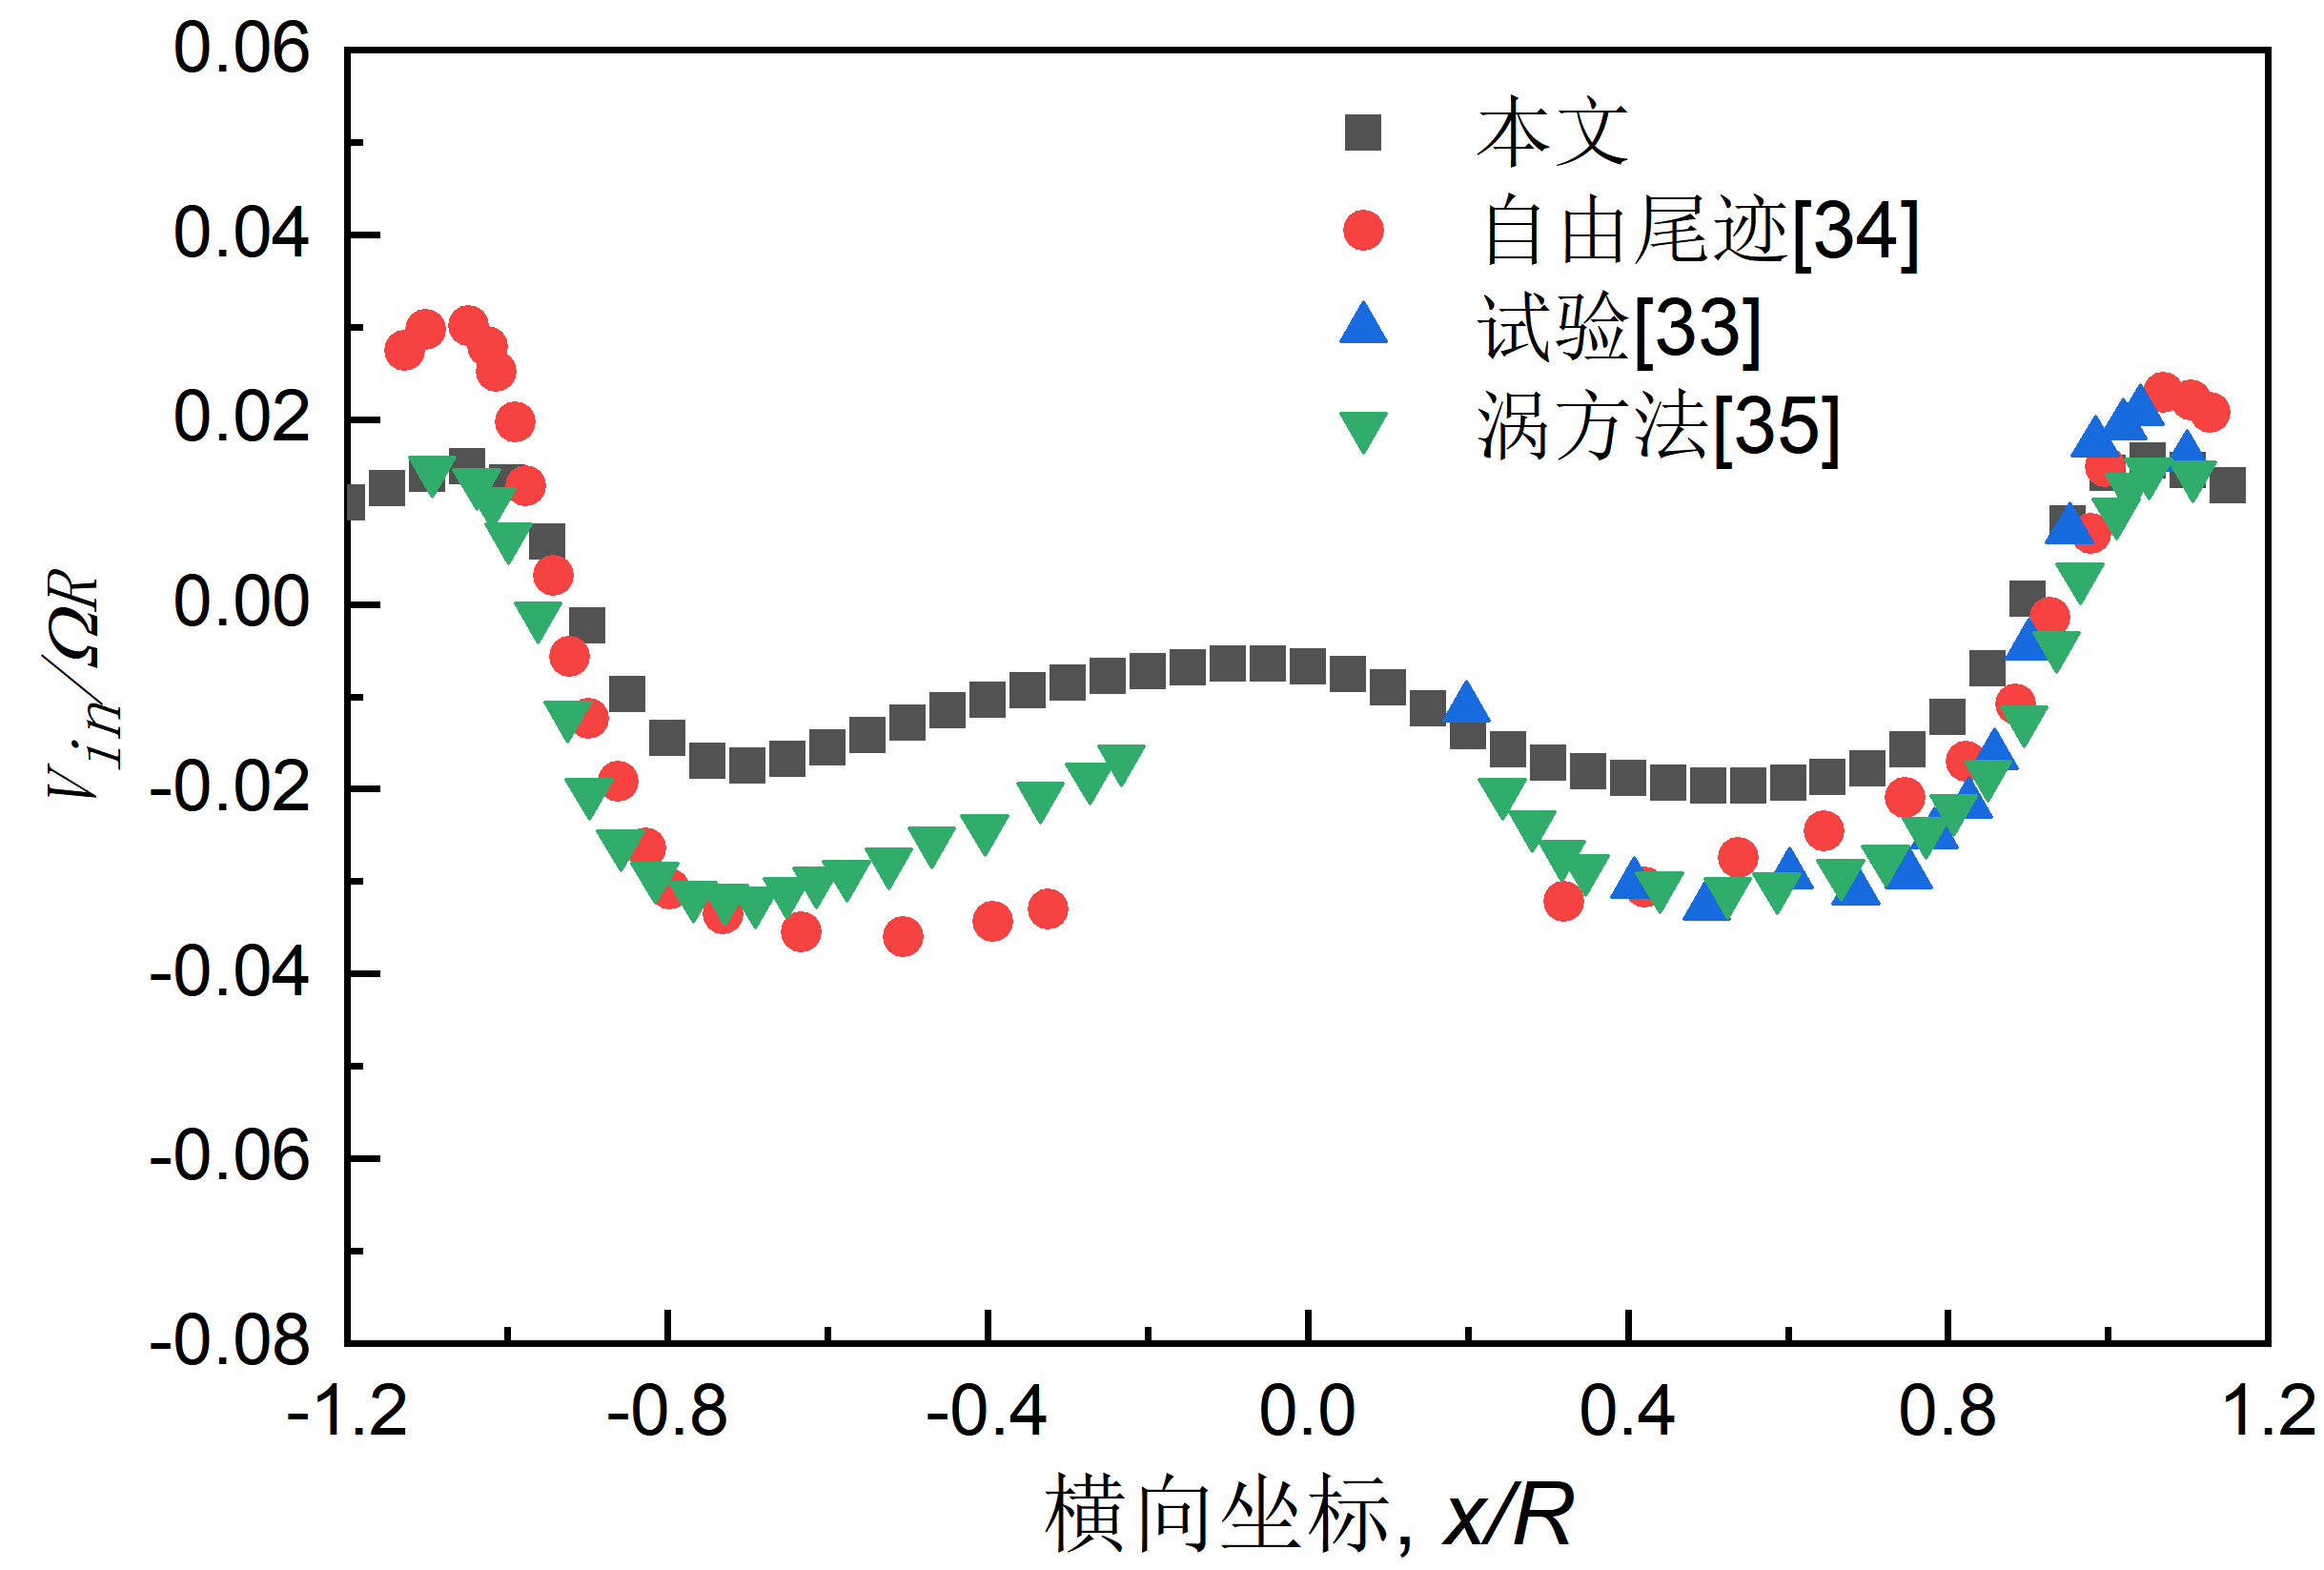
\includegraphics[width=7cm]{chap_2_5_3_2_3.png}}\\
    \caption{Scaled-model旋翼计算结果与试验结果对比}
    \label{fig:chap2_5_3_2_2}
\end{figure}

\subsubsection{前飞状态下的Scaled-model旋翼}
Scaled-model旋翼的风洞试验数据见参考文献\cite{elliott1988inflow}。Scaled-model旋翼有4片桨叶,桨叶翼型为NACA0012。旋翼转速为2113 rpm,旋翼半径为0.861 m,桨叶弦长为0.066 m,线性负扭为-8\degree。将桨距写为傅里叶形式,其常数项、一阶余弦项、一阶正弦项分别为6.3\degree,-2.1\degree,2\degree。桨盘迎角为3\degree。前飞速度为28.5 m/s,对应前进比0.15。

前飞状态下的Scaled-model旋翼尾迹见图\ref{fig:chap2_5_3_2_1}。基于上述涡方法,可以捕捉到前行侧、后行侧的初始桨尖涡以及后缘卷起的桨尖涡。

图\ref{fig:chap2_5_3_2_2}给出了纵向、横向的入流速度。与基于自由尾迹的计算结果\cite{bhagwat2001transient}相比,本文结果与试验值间误差更小。此外,可以看出,本文结果与参考文献\cite{tan2013simulating}中的结果基本一致,这也体现了本文提出的涡方法的有效性和可行性。

\subsubsection{纵列式双旋翼}
本文用来验证的纵列式双旋翼试验数据来自参考文献\cite{dingeldein1954wind}。其中,纵列式双旋翼两旋翼轴间的纵向距离为4.724 m,垂向、侧向距离均为0。前后旋翼桨叶无负扭、无尖削,翼型为NACA0012。旋翼半径为2.286 m,实度为0.054。
\begin{figure}[!htb]  
  \subfloat[悬停]{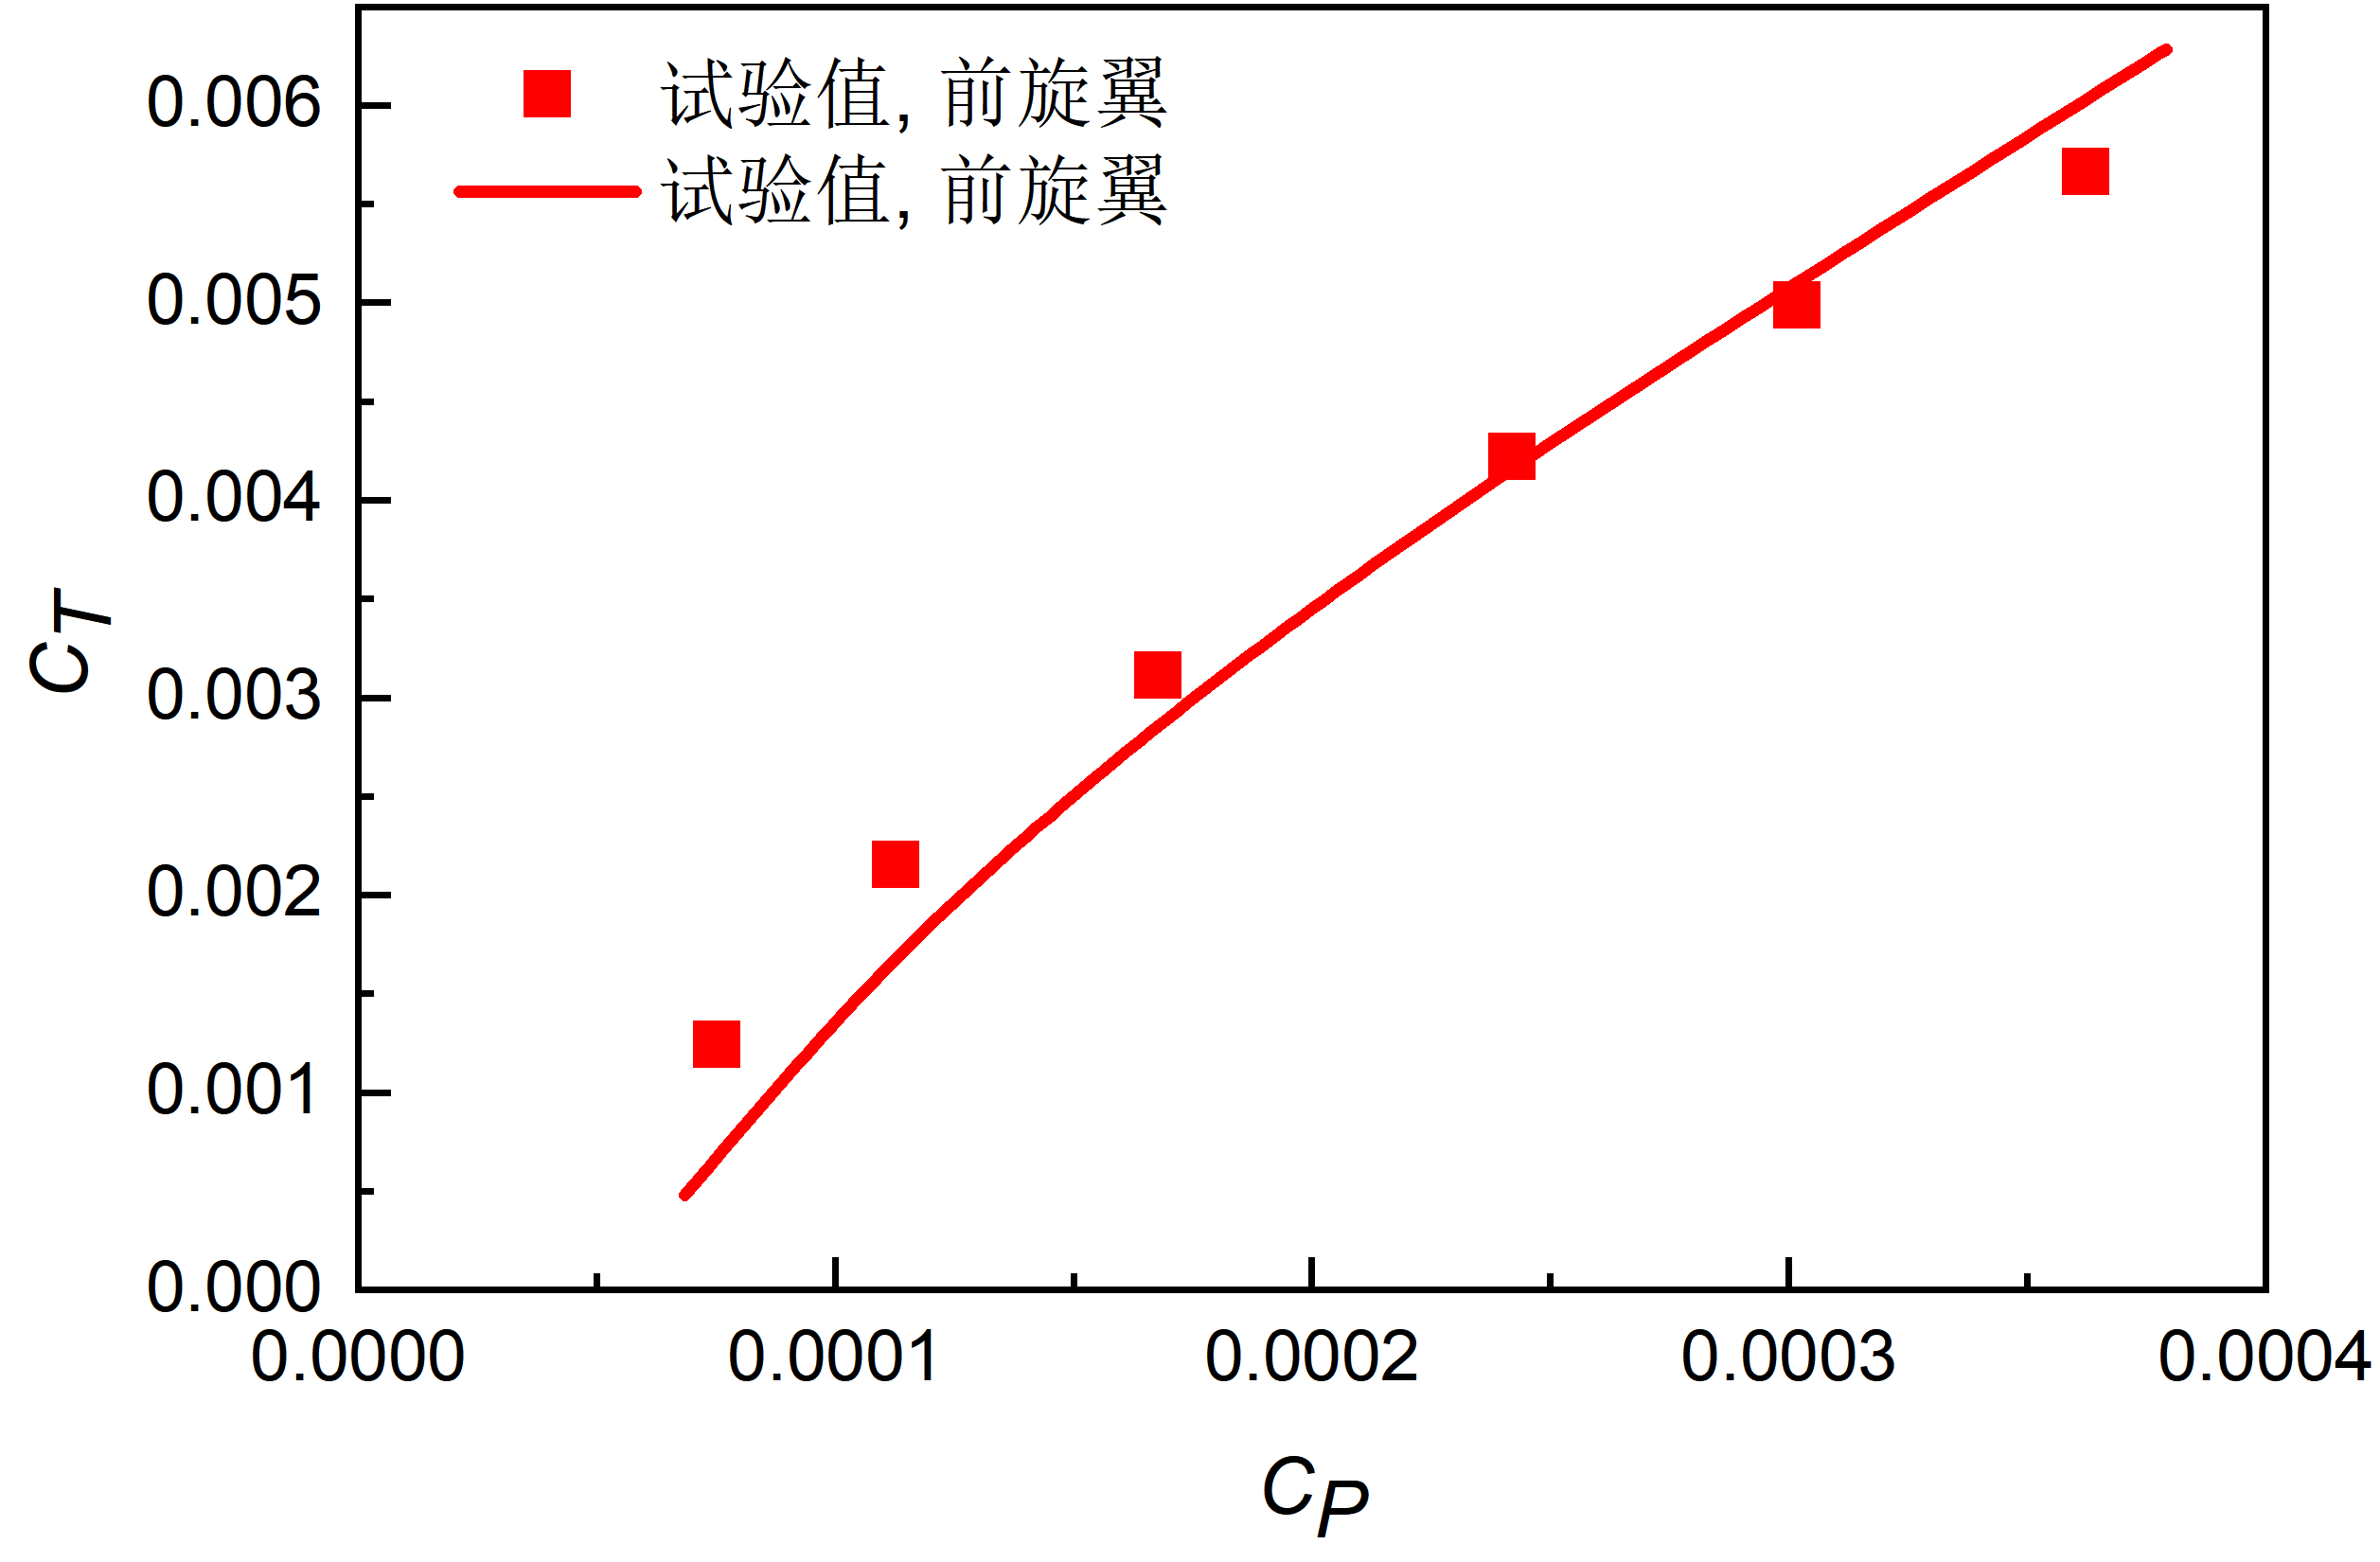
\includegraphics[width=7cm]{chap_2_5_3_3_1.png}}\quad
    \subfloat[定常平飞,$C_T=0.0034$]{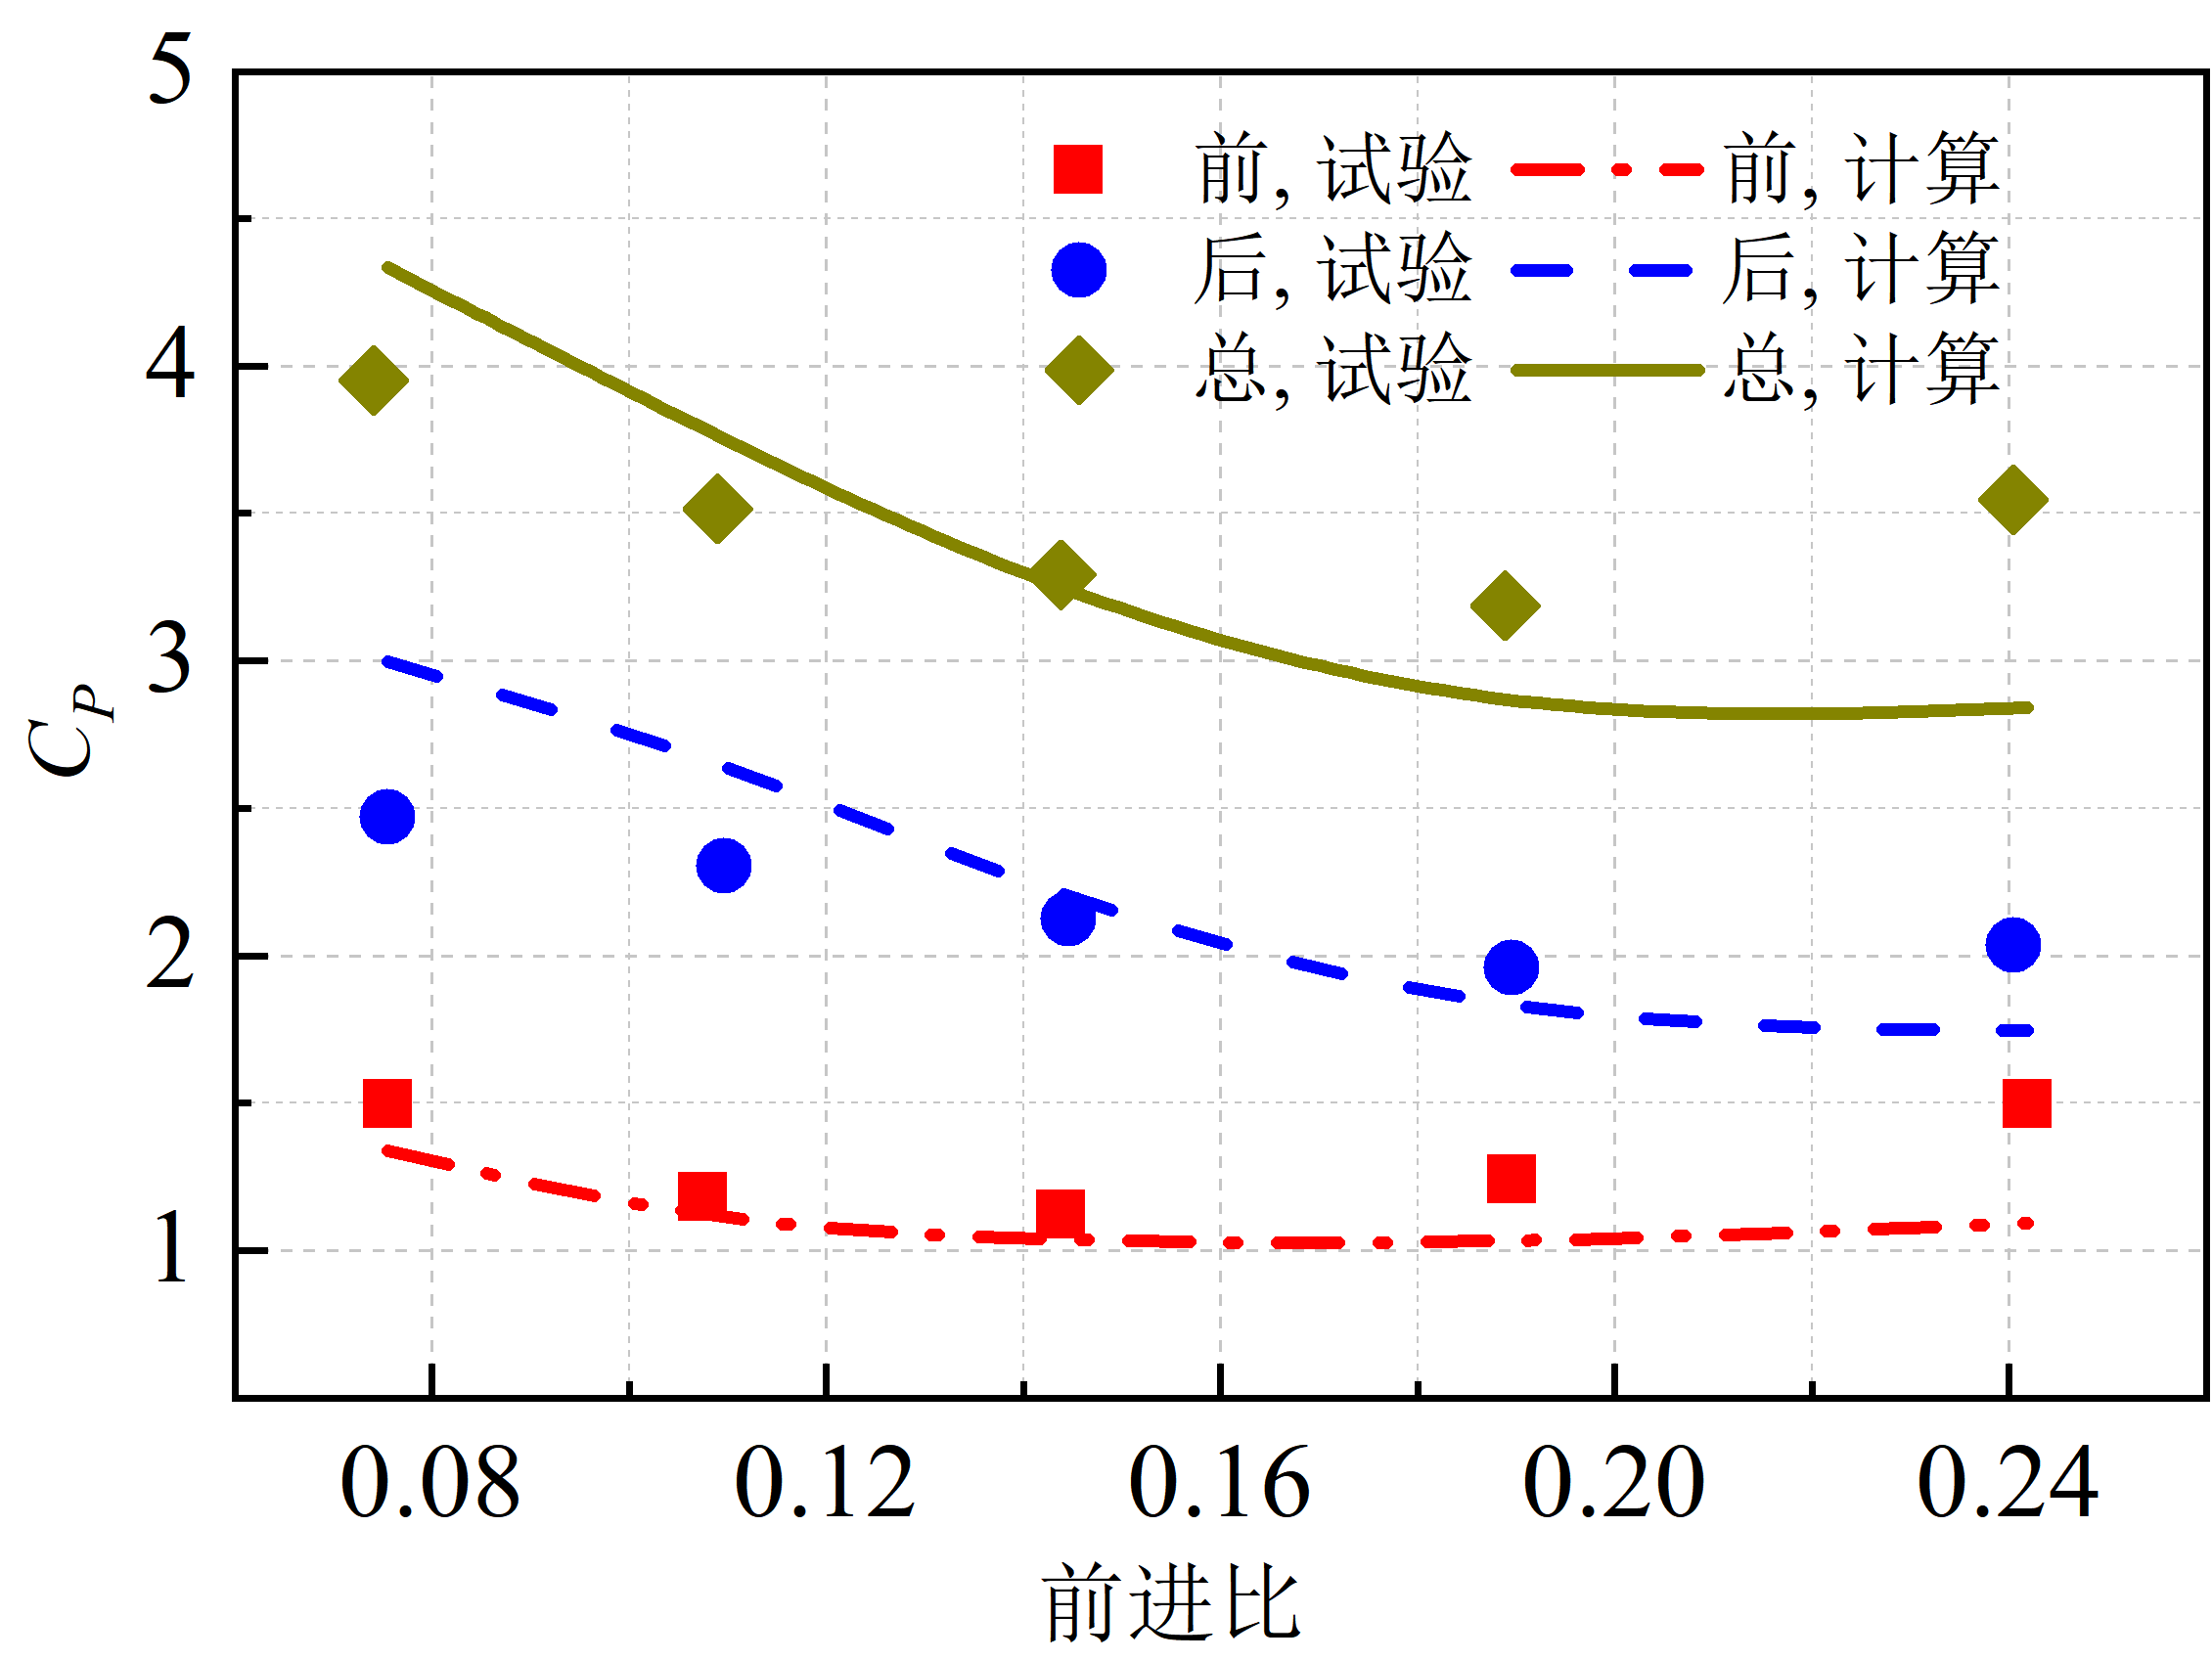
\includegraphics[width=6.7cm]{chap_2_5_3_3_2.png}}\\
    \caption{纵列式双旋翼计算结果与试验结果对比}
    \label{fig:chap2_5_3_3_1}
\end{figure}

考虑到悬停时前后旋翼位置对称、入流相等,前后旋翼性能一致。因此悬停时本文以前旋翼为例开展了分析,见图\ref{fig:chap2_5_3_3_1}(a)。可以看出,当$C_P$大于0.015时,基于涡方法计算得到的$C_T$与试验值间的相对误差小于10\%。$C_T$、$C_P$的值较小时,尽管相对误差较大,但计算值和试验值的整体趋势是一致的。

见图\ref{fig:chap2_5_3_3_1}(b),前飞时以$C_T$等于0.0034时的计算值与试验值为例开展对比分析。总功率消耗为前后旋翼功率消耗的和。可以看出,后旋翼的功率消耗比前旋翼的大,这是由于后旋翼除了受到自由流场作用外,还受到前旋翼的下洗流干扰。此外,当前进比大于0.2时,虽然前旋翼功率与试验结果之间相对误差较大,但整体趋势是一致的。

\section{直升机协同吊挂系统动力学模型}

\section{本章小结}
% \chapter{直升机协同吊挂系统动力学特性及气动干扰分析}
\section{引言}
\section{分层配平法}
\subsection{吊挂物层配平}
\subsection{吊索层优化配平}
\subsection{直升机层差量配平}
\section{配平结果分析}
\section{操纵性分析}
\section{稳定性分析}
\section{气动干扰及其导致的性能变化}
直升机协同吊挂系统是典型的近距离飞行,直升机间、直升机与吊挂物之间、直升机各部件间均存在气动干扰。其中,以前飞时前后排列的直升机间的干扰最为严重。对气动干扰进行分析,可以了解气动干扰产生的机理,有利于减少功率消耗,获得最佳队形,提升系统性能。
\subsection{数值计算条件}
\begin{table}[htb!]
  \caption{直升机1和直升机4的配平结果\label{table:chap_2_1}}
  \begin{tabular}{ccccccccccccc}
    \toprule
    前进比&\multicolumn{2}{c}{0}& \multicolumn{2}{c}{0.04}&\multicolumn{2}{c}{0.06}&\multicolumn{2}{c}{0.08}&\multicolumn{2}{c}{0.1}&\multicolumn{2}{c}{0.14}\\   
    直升机&1&4&1&4&1&4&1&4&1&4&1&4\\
    \midrule
    $\theta_{0,F}$ (\degree)&5.5&5.7&4.0&5.0&3.7&4.8&4.2&4.6&4.1&4.6&4.6&5.2\\
    ${A_{1,F}}$ (\degree)&0.0&0.0&0.4&0.9&0.9&1.2&0.7&1.4&0.9&1.2&1.0&1.0\\
    ${a_{0,F}}$ (\degree)&1.7&1.8&1.4&1.7&1.5&1.7&1.8&1.6&1.8&1.6&1.8&1.5\\
    ${a_{1,F}}$ (\degree)&0.0&0.0&0.6&1.0&1.2&1.5&1.2&1.7&1.5&1.7&1.9&1.9\\
    $\theta_{0,R}$ (\degree)& 5.6 & 5.8 & 4.5 & 5.3 & 4.4 & 5.7 & 4.7 & 5.8 & 4.9 & 5.7 & 5.4 & 6.1\\
    ${A_{1,R}}$ (\degree)& 0.0 & 0.0 & 0.4 & 0.7 & 0.8 & 1.1 & 0.7 & 1.2 & 0.7 & 1.1 & 0.7 & 0.9 \\
    ${a_{0,R}}$ (\degree)& 1.7 & 1.8 & 1.7 & 1.8 & 1.8 & 2.1 & 2.0 & 2.1 & 2.2 & 2.1 & 2.2 & 2.0 \\
    ${a_{1,R}}$ (\degree)& 0.0 & 0.0 & 0.7 & 1.0 & 1.2 & 1.5 & 1.3 & 1.8 & 1.6 & 1.8 & 2.1 & 2.1 \\
    $\theta$ (\degree)& 3.4 & -3.9 & 2.8 & -5.3 & 1.8 & -7.2 & 0.5 & -7.7 & -0.8 & -8.9 & -4.3 & -11.4 \\
    \bottomrule
  \end{tabular}
\end{table}
协同吊挂系统的气动干扰研究是在稳定飞行状态下开展的。稳定飞行状态下的状态量基于前文提出的混合优化配平算法配平得到。
本文研究的四纵列式直升机协同吊挂系统是“2-lead”队形的,假设吊挂负载均匀分配给各直升机,那么稳定飞行状态下后侧直升机(直升机1、2)的纵向配平量相等,前侧直升机(直升机3、4)的纵向配平量相等。下表以直升机1、直升机3为例给出了配平结果。其中,${\theta _{0,F}}$、${\theta _{0,R}}$分别为前、后旋翼的总距,$\theta $是俯仰角,${A_{1,F}}$、${A_{1,R}}$是横向周期变距,${a_{0,F}}$、${a_{0,R}}$是前、后旋翼挥舞角写成傅里叶级数时的常数项,${a_{1,F}}$、${a_{1,R}}$是前、后旋翼挥舞角写成傅里叶级数时的cos项。值得一提的是,纵列式直升机纵向运动是通过前后旋翼的总距差动实现的,所以纵向周期变距等于0。此外,直升机1和直升机4的滚转角为-4 \degree,直升机2和直升机3的滚转角为4 \degree。直升机1、2、3、4和吊挂物在地轴系下的位置依次为[-1.8, -1.8, -3.7],[-1.8, 1.8, -3.7],[1.8, 1.8, -3.7],[1.8, -1.8, -3.7] 和 [0, 0, 0]。

值得一提的是,以稳定飞行状态为基础计算气动干扰是必要的。若没有配平,而是随意选择各直升机姿态角和旋翼操纵量开展气动干扰分析,此时的计算结果是没有意义的,不能体现直升机协同吊挂系统的真实飞行状态。表\ref{table:chap_2_1}所示的配平量为涡方法提供了系统初始状态量,保证了气动干扰分析和性能计算的可靠度。

\begin{figure}[!htb]
  \centering
  \subfloat[X-Z平面]{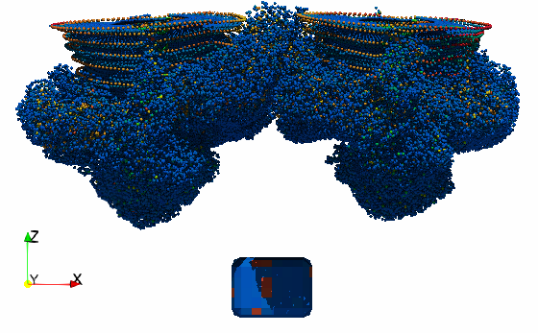
\includegraphics[width=6cm]{fig/figure_chap3/chap_3_5_1_1_1.png}}\quad 
  \subfloat[X-Y平面]{\includegraphics[width=5cm]{fig/figure_chap3/chap_3_5_1_1_2.png}}\\
  \caption{悬停时直升机协同吊挂系统尾迹结构}
  \label{fig:chap3_5_1_1_1}
\end{figure}

\begin{figure}[!htb]
  \centering
  \subfloat[X-Z平面]{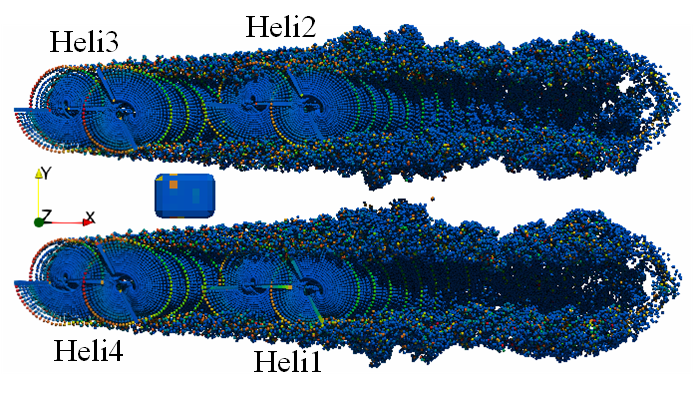
\includegraphics[width=6cm]{fig/figure_chap3/chap_3_5_1_2_1.png}}\quad 
  \subfloat[X-Y平面]{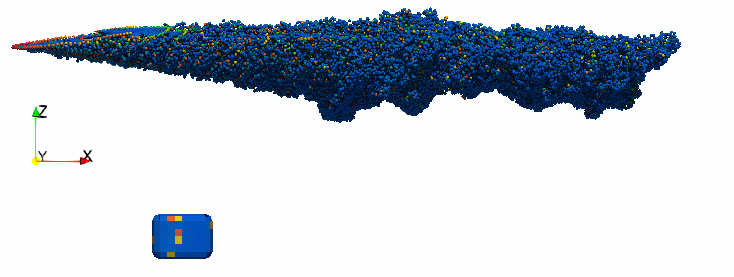
\includegraphics[width=8cm]{fig/figure_chap3/chap_3_5_1_2_2.png}}\\
  \caption{前进比0.1时直升机协同吊挂系统尾迹结构}
  \label{fig:chap3_5_1_1_2}
\end{figure}

\subsection{不同飞行速度下的气动干扰}
基于表\ref{table:chap_2_1}中的配平结果,开展了稳定飞行状态下的气动干扰特性分析。图\ref{fig:chap3_5_1_1_1}和图\ref{fig:chap3_5_1_1_2}分别给出了悬停、前进比0.1(前飞速度10 m/s)时的尾迹结构。可以看出,悬停时四个纵列式直升机间几乎没有干扰。前进比0.1时存在气动干扰,其中以前后排列的直升机间的干扰最大。此外,可以发现无论是悬停还是前进比0.1时,吊挂物都没有浸入旋翼尾迹中。这说明本文研究的四纵列式直升机协同吊挂系统,直升机对吊挂物的气动干扰不大。并且,从表\ref{table:chap_2_1}的配平结果、图\ref{fig:chap3_5_1_1_1}和图\ref{fig:chap3_5_1_1_2}的尾迹结构可以看出,直升机1和2的配平结果及气动干扰情况是相似的,直升机3和4的配平结果及气动干扰情况也是相似的。因此,下文以直升机1和直升机4为例开展讨论和分析。

\begin{figure}[!htb]
  \centering
  \subfloat[悬停时XY截面的速度场]{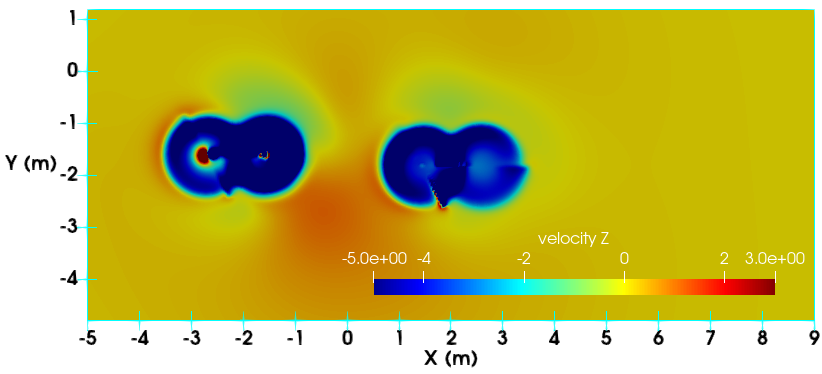
\includegraphics[width=5.5cm]{fig/figure_chap3/chap_3_5_1_3.png}}\quad 
  \subfloat[悬停时XZ截面的速度场]{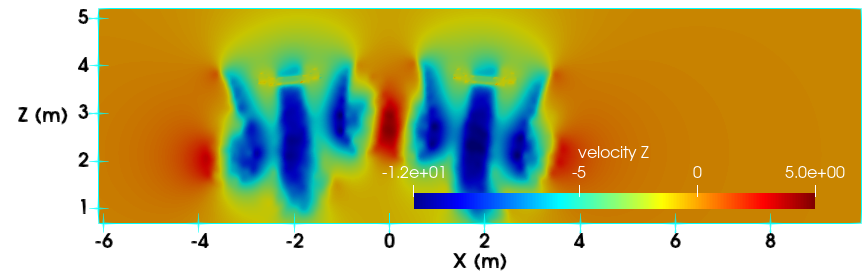
\includegraphics[width=8.5cm]{fig/figure_chap3/chap_3_5_1_4.png}}\\
  \subfloat[前飞速度6 m/s时XY截面的速度场]{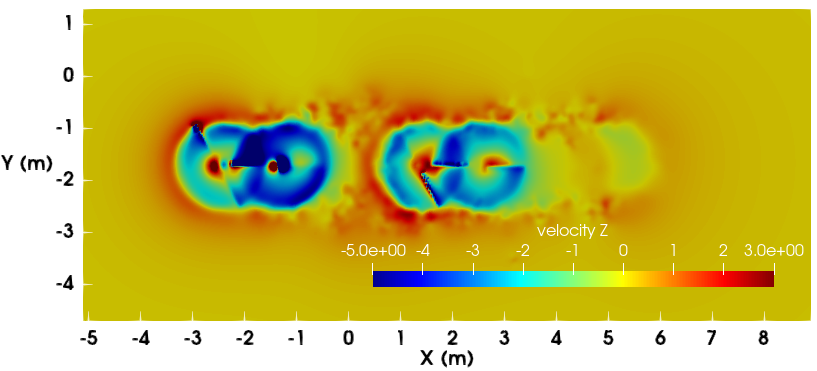
\includegraphics[width=5.5cm]{fig/figure_chap3/chap_3_5_1_5.png}}\quad 
  \subfloat[前飞速度6 m/s时XZ截面的速度场]{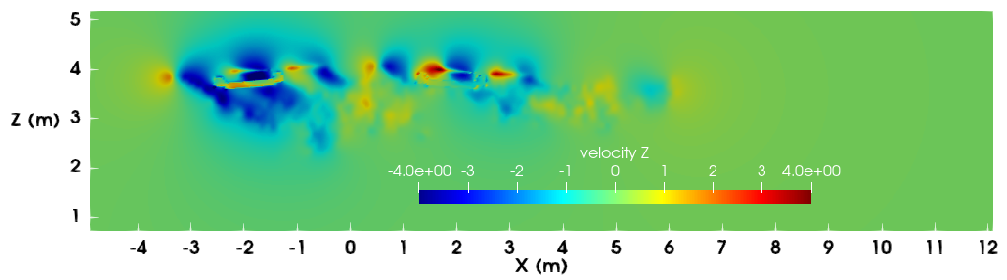
\includegraphics[width=8.5cm]{fig/figure_chap3/chap_3_5_1_6.png}}\\
  \subfloat[前飞速度12 m/s时XY截面的速度场]{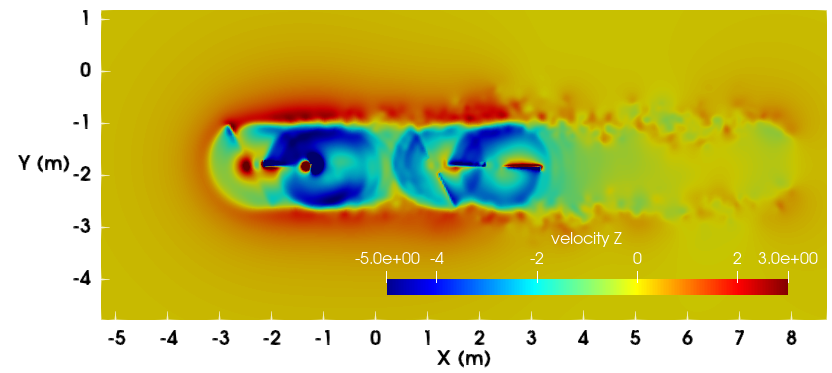
\includegraphics[width=5.5cm]{fig/figure_chap3/chap_3_5_1_7.png}}\quad 
  \subfloat[前飞速度12 m/s时XZ截面的速度场]{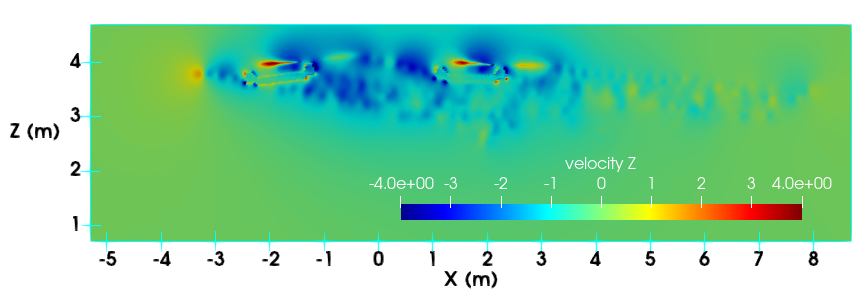
\includegraphics[width=8.5cm]{fig/figure_chap3/chap_3_5_1_8.png}}\\
  \caption{直升机协同吊挂系统不同飞行状态下的速度场}
  \label{fig:chap3_5_1_2}
\end{figure}
 
图\ref{fig:chap3_5_1_2}给出了直升机1和直升机4不同飞行状态下的速度场。悬停时,如图\ref{fig:chap3_5_1_2}(a)(b)所示,旋翼下洗速度主要存在于桨盘到桨盘2倍旋翼直径以下的区域。上洗速度是涡扩散和上卷引起的。其中,由于前后直升机尾迹的重合,坐标(0,0,3m)处的上洗速度是(±3.8m,0,2m)处的2倍。尾迹倾斜与直升机自身的姿态角有关。悬停时直升机1和直升机4的姿态角分别为3.4 \degree 和-3.9 \degree,所以直升机4的尾迹向左倾斜,直升机1的尾迹向右倾斜。

前进比0.06时,如图\ref{fig:chap3_5_1_2}(c)(d)所示,尾迹朝来流方向倾斜,由于上卷桨尖涡的作用,给纵列式直升机1的前旋翼带来了一定的上洗速度。这尽管有利于增加直升机1千旋翼的迎角,但上卷的桨尖涡作用会给旋翼带来更复杂的工作环境。前进比0.1时,随着飞行速度的增加,直升机4的旋翼下洗流对直升机1的干扰越来越大。相比无干扰时,这势必会导致直升机1旋翼拉力的减小和功率消耗的增加。

可见,对于本文研究的四纵列式直升机协同吊挂系统,悬停时直升机之间、直升机与吊挂物之间几乎不存在气动干扰。随着飞行速度的增加,气动干扰变得越来越严重,以前后排列的直升机间的干扰更甚。此外,可以发现协同吊挂系统间的气动干扰比较复杂,且不同前飞速度下对性能的影响往往是不同的。为了减少协同吊挂系统中的气动干扰、提高性能,下文重点分析气动干扰的变化及其影响因子。其中,为分析方便,固定前进比为0.1,对应协同吊挂系统中气动干扰较为严重的情况。

\begin{figure}
  \centering
  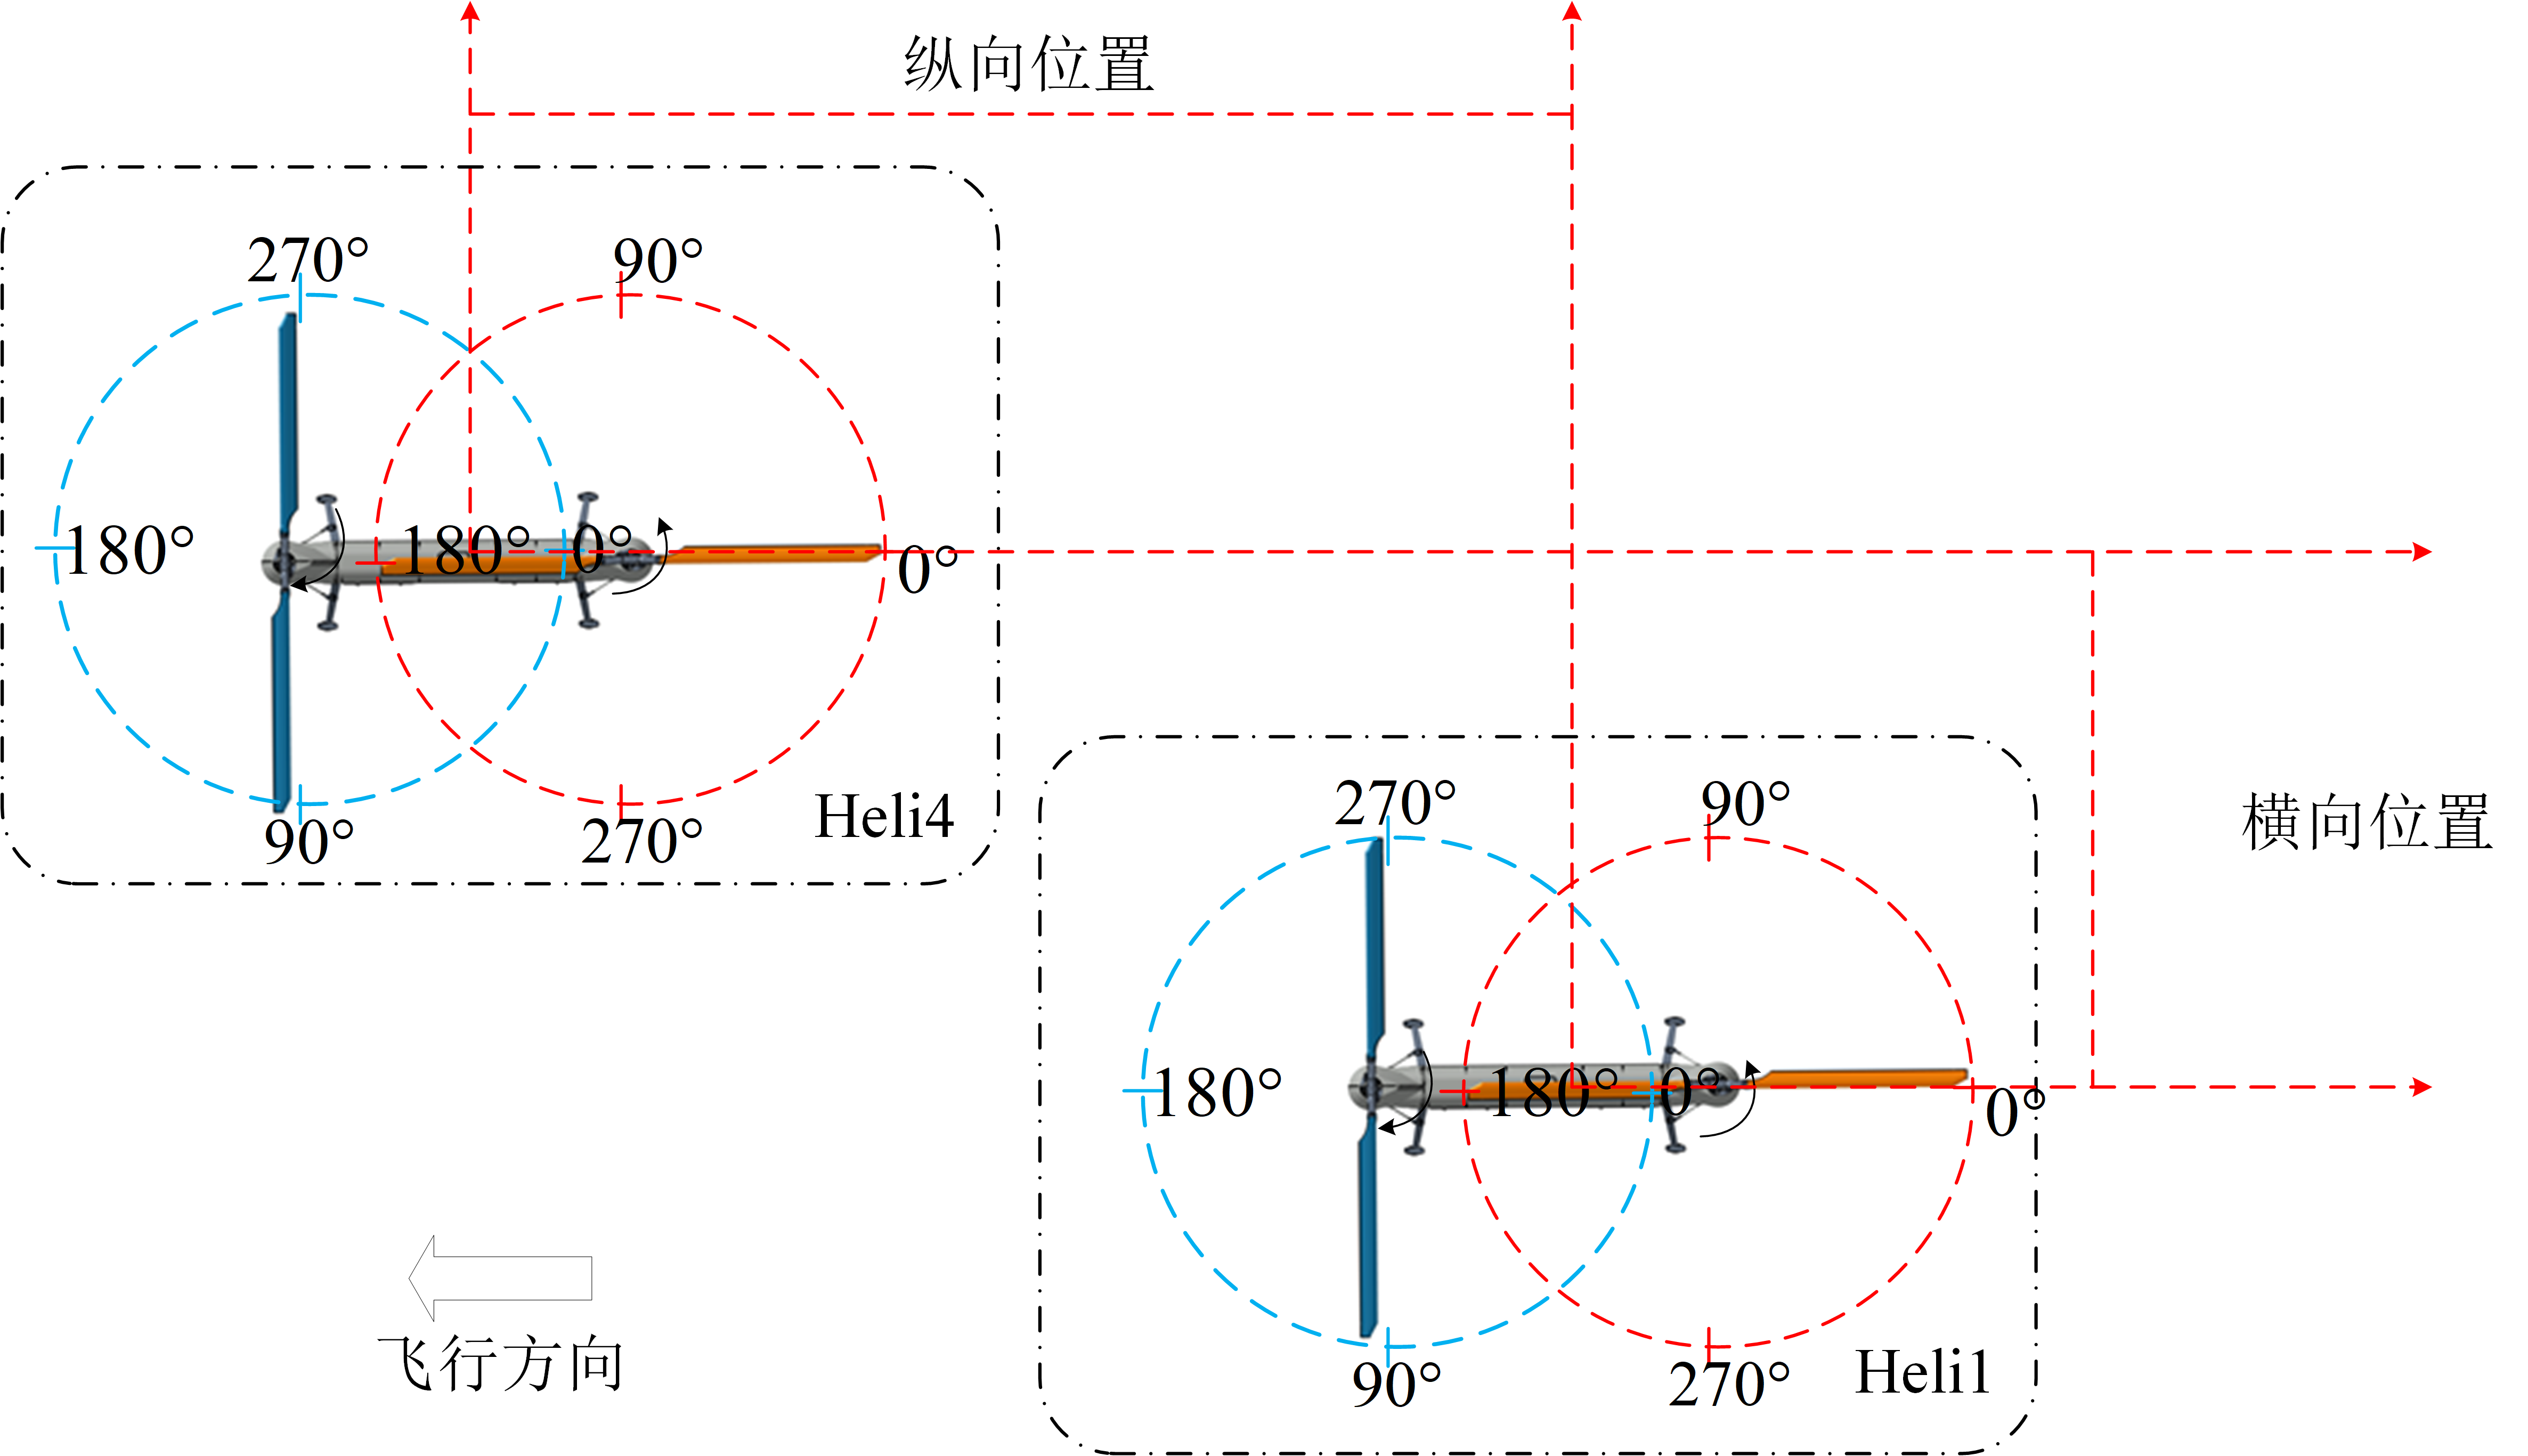
\includegraphics[width=10cm]{fig/figure_chap3/chap_3_5_1_9.png}
  \caption{直升机1和直升机4的相对位置定义\label{fig:chap3_5_1_3}}
\end{figure}
 
纵列式直升机前后旋翼的转向、直升机1与直升机4的纵向距离、直升机1与直升机4的侧向距离定义见图\ref{fig:chap3_5_1_3}。

\subsection{不同横向相对位置下气动干扰及性能的变化}
本小节给出了气动干扰随直升机横向相对位置的变化,其中直升机1相对直升机4的横向相对位置变化范围为-1.5到1.5倍的旋翼直径。相对位置为-1.5倍的旋翼直径时,表示直升机1在直升机4的左后方;相对位置为1.5倍的旋翼直径时,表示直升机1在直升机4的右后方。

图\ref{fig:chap3_5_2_1}给出了直升机协同吊挂系统三个典型横向相对位置下的涡度场。可以看出,在基本配置中,直升机1完全沉浸在直升机4的尾流中。当左移0.5倍的旋翼直径时,只有直升机1前旋翼的后行侧、后旋翼的前行侧沉浸在直升机4的尾流中。随着横向距离的进一步增加,如\ref{fig:chap3_5_2_1}(c)所示,直升机1和直升机4之间几乎没有干扰。

此外,值得一提的是,直升机1相对直升机4右移时的干扰情况与左移时类似。唯一不同的是,当右移0.5到1倍的旋翼直径时,直升机1前旋翼的前行侧、后旋翼的后行侧沉浸在直升机4的尾流中。
\begin{figure}[!htb]
  \centering
  \subfloat[基本配置]{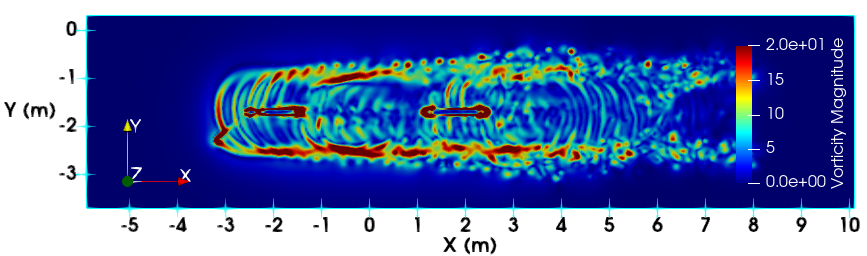
\includegraphics[width=7cm]{fig/figure_chap3/chap_3_5_2_1.png}}\\ 
  \subfloat[左移0.5倍旋翼直径]{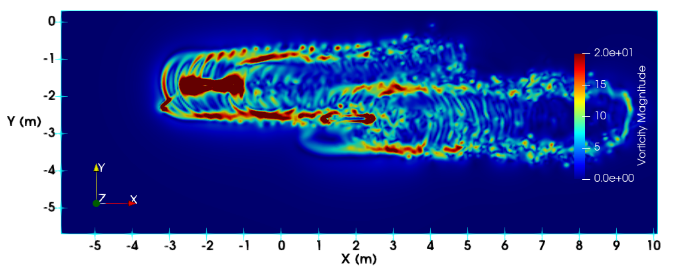
\includegraphics[width=7cm]{fig/figure_chap3/chap_3_5_2_2.png}}\quad
  \subfloat[左移一倍旋翼直径]{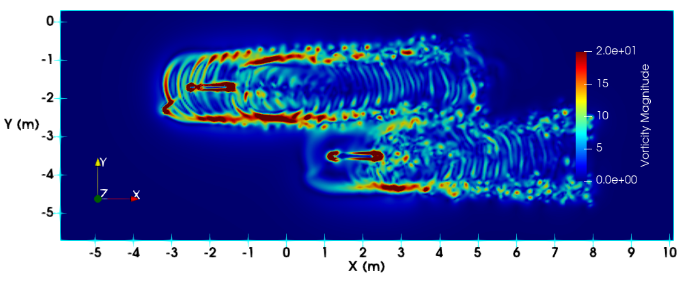
\includegraphics[width=7cm]{fig/figure_chap3/chap_3_5_2_3.png}}
  \caption{直升机协同吊挂系统不同横向相对位置下的涡度场}
  \label{fig:chap3_5_2_1}
\end{figure}

图\ref{fig:chap3_5_2_2}(a)给出了直升机1前旋翼0.75R处的截面力。可以看出,基本配置、左移0.5倍旋翼直升机、左移1倍旋翼直径三种情况下,方位角100 \degree 到 250 \degree 期间,截面力有较大差距。基本配置中,直升机1完全沉浸在直升机4的尾流中,所以截面力远远比其他两种情况下小。左移0.5倍的旋翼直径时,方位角200 \degree 到 250 \degree 间的截面力远远小于方位角100 \degree 到 170 \degree 间的截面力。左移1倍的旋翼直径时,各个方位角的力均比其他两种情况下大。上述变化与不同相对侧向位置下的气动干扰变化相一致。

此外,根据图\ref{fig:chap3_5_2_2}(b)直升机1后旋翼0.75R处的截面力可知,相对侧向位置对直升机1后旋翼的影响较小。这是由于直升机1后旋翼受到前旋翼尾流的影响远远比受到直升机4的尾流影响大。

\begin{figure}[!htb]
  \centering
  \subfloat[前旋翼]{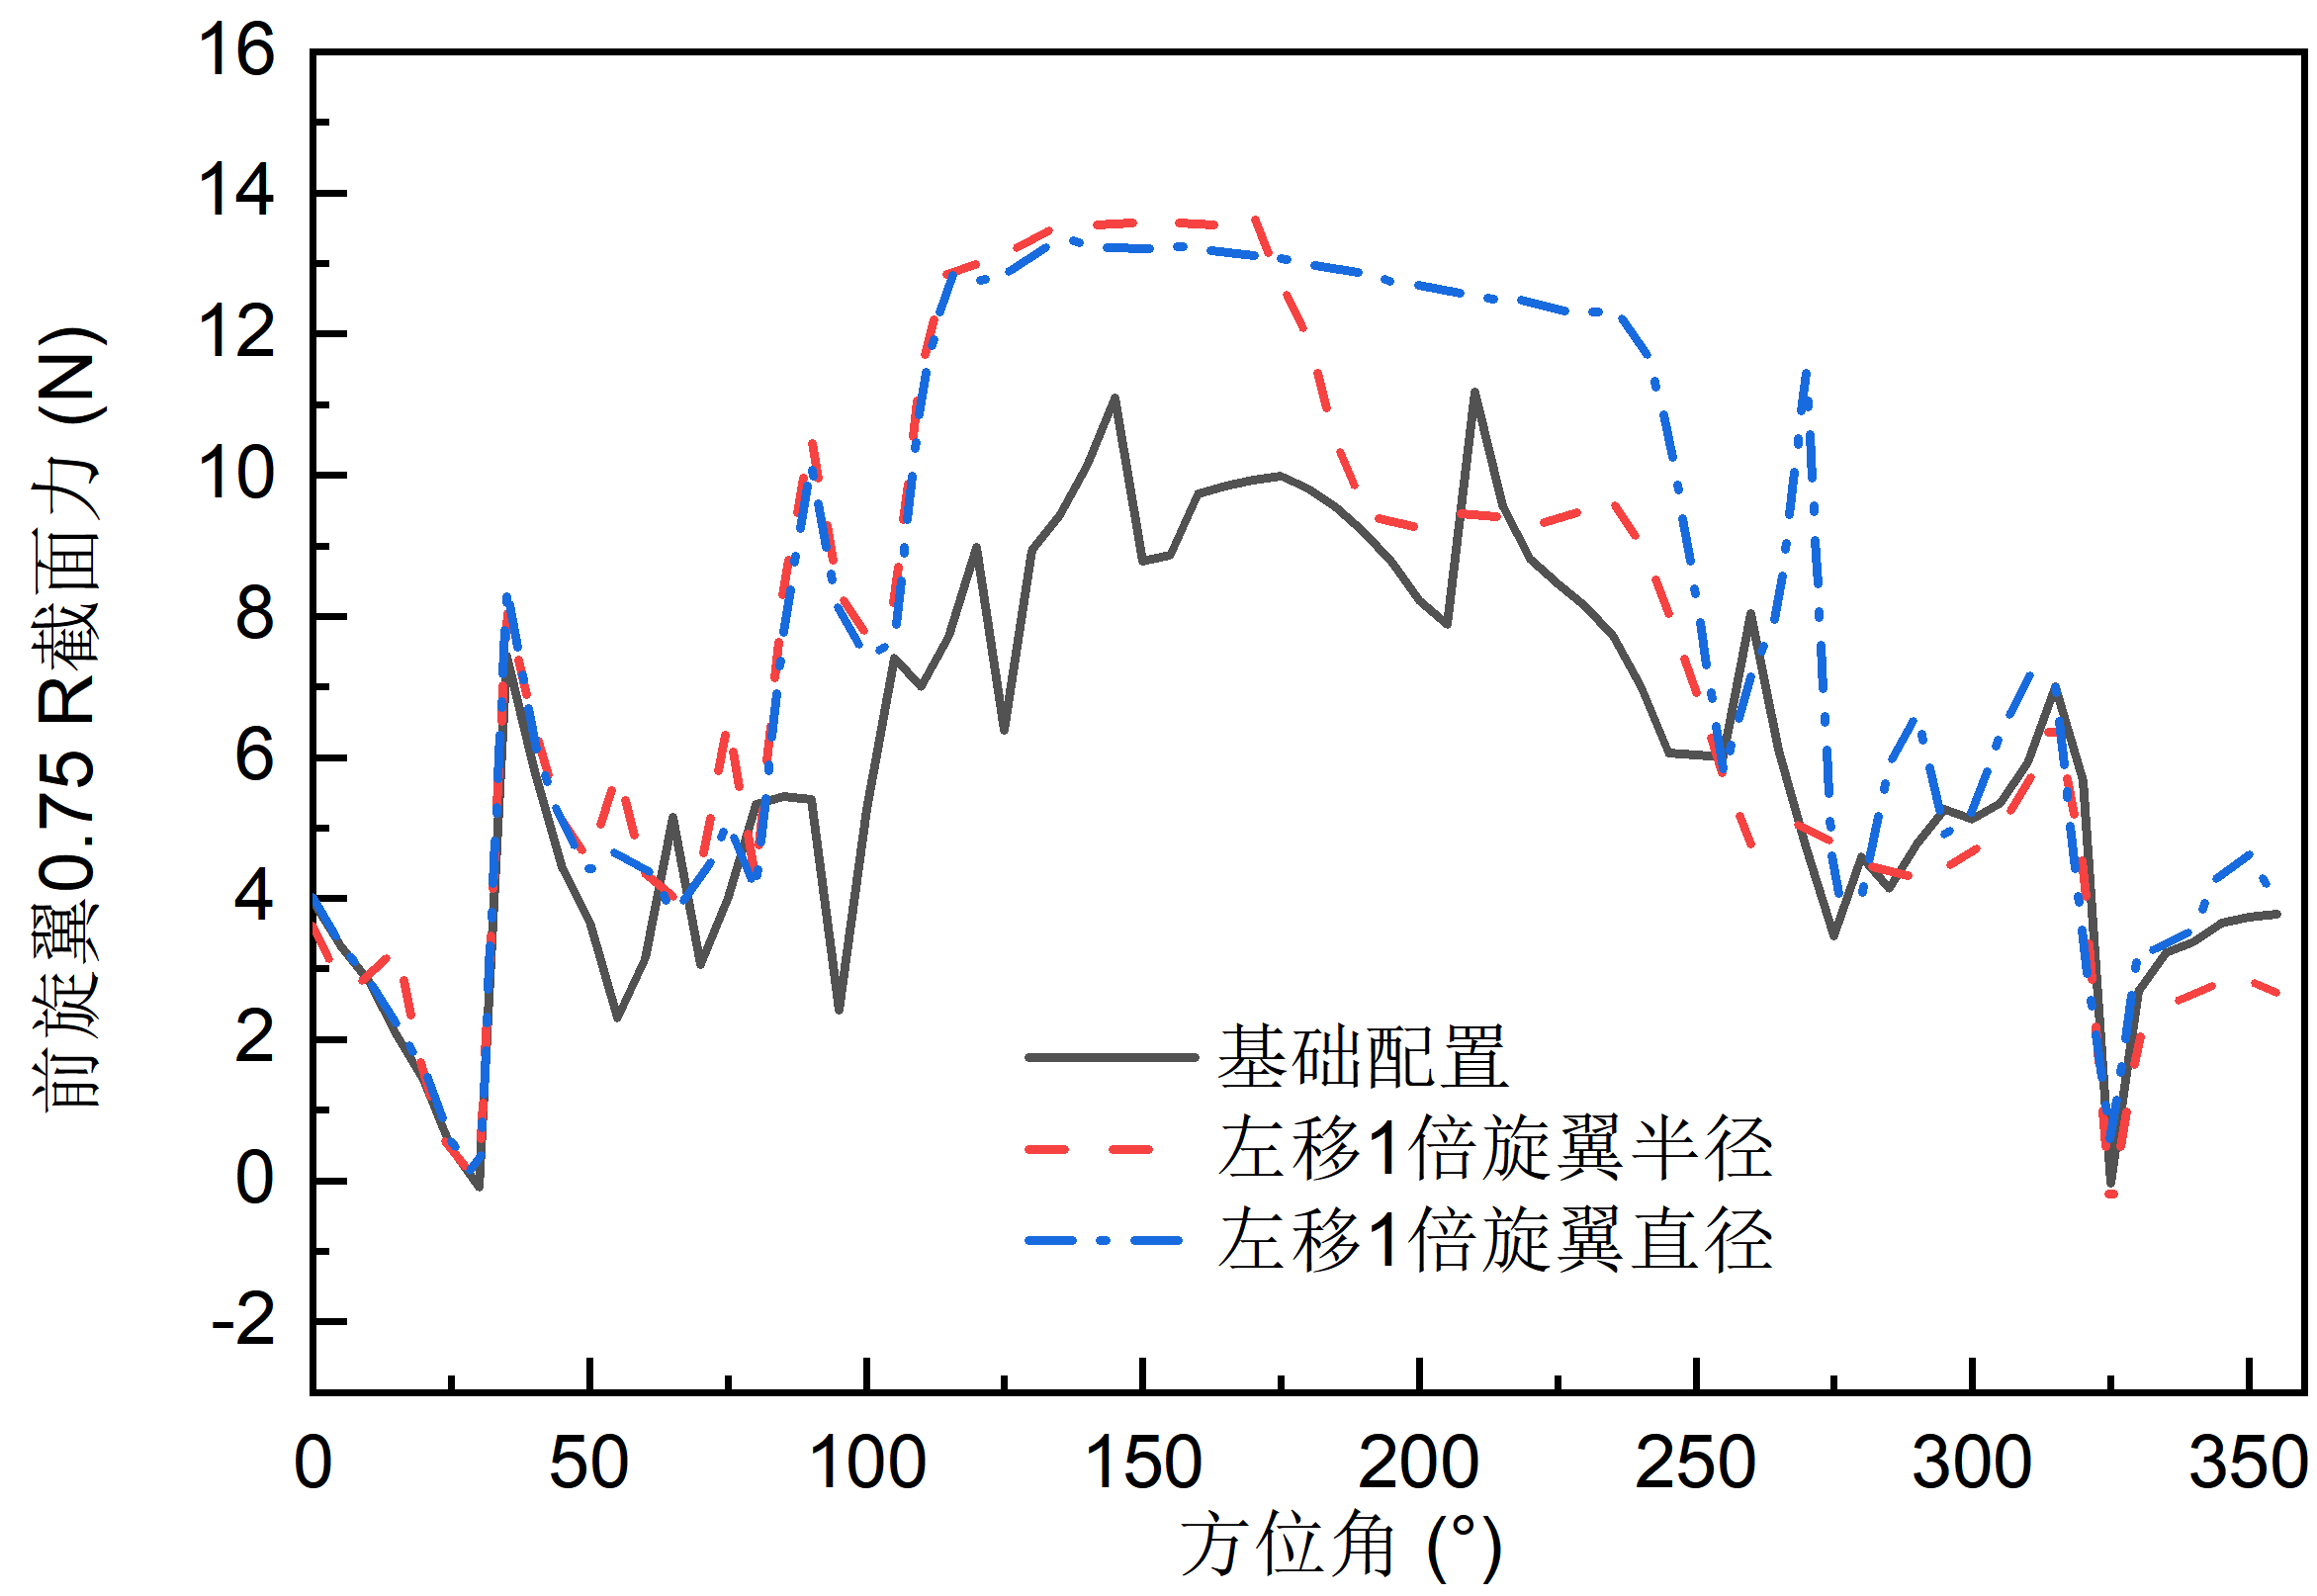
\includegraphics[width=7cm]{fig/figure_chap3/chap_3_5_2_4.png}}\quad
  \subfloat[后旋翼]{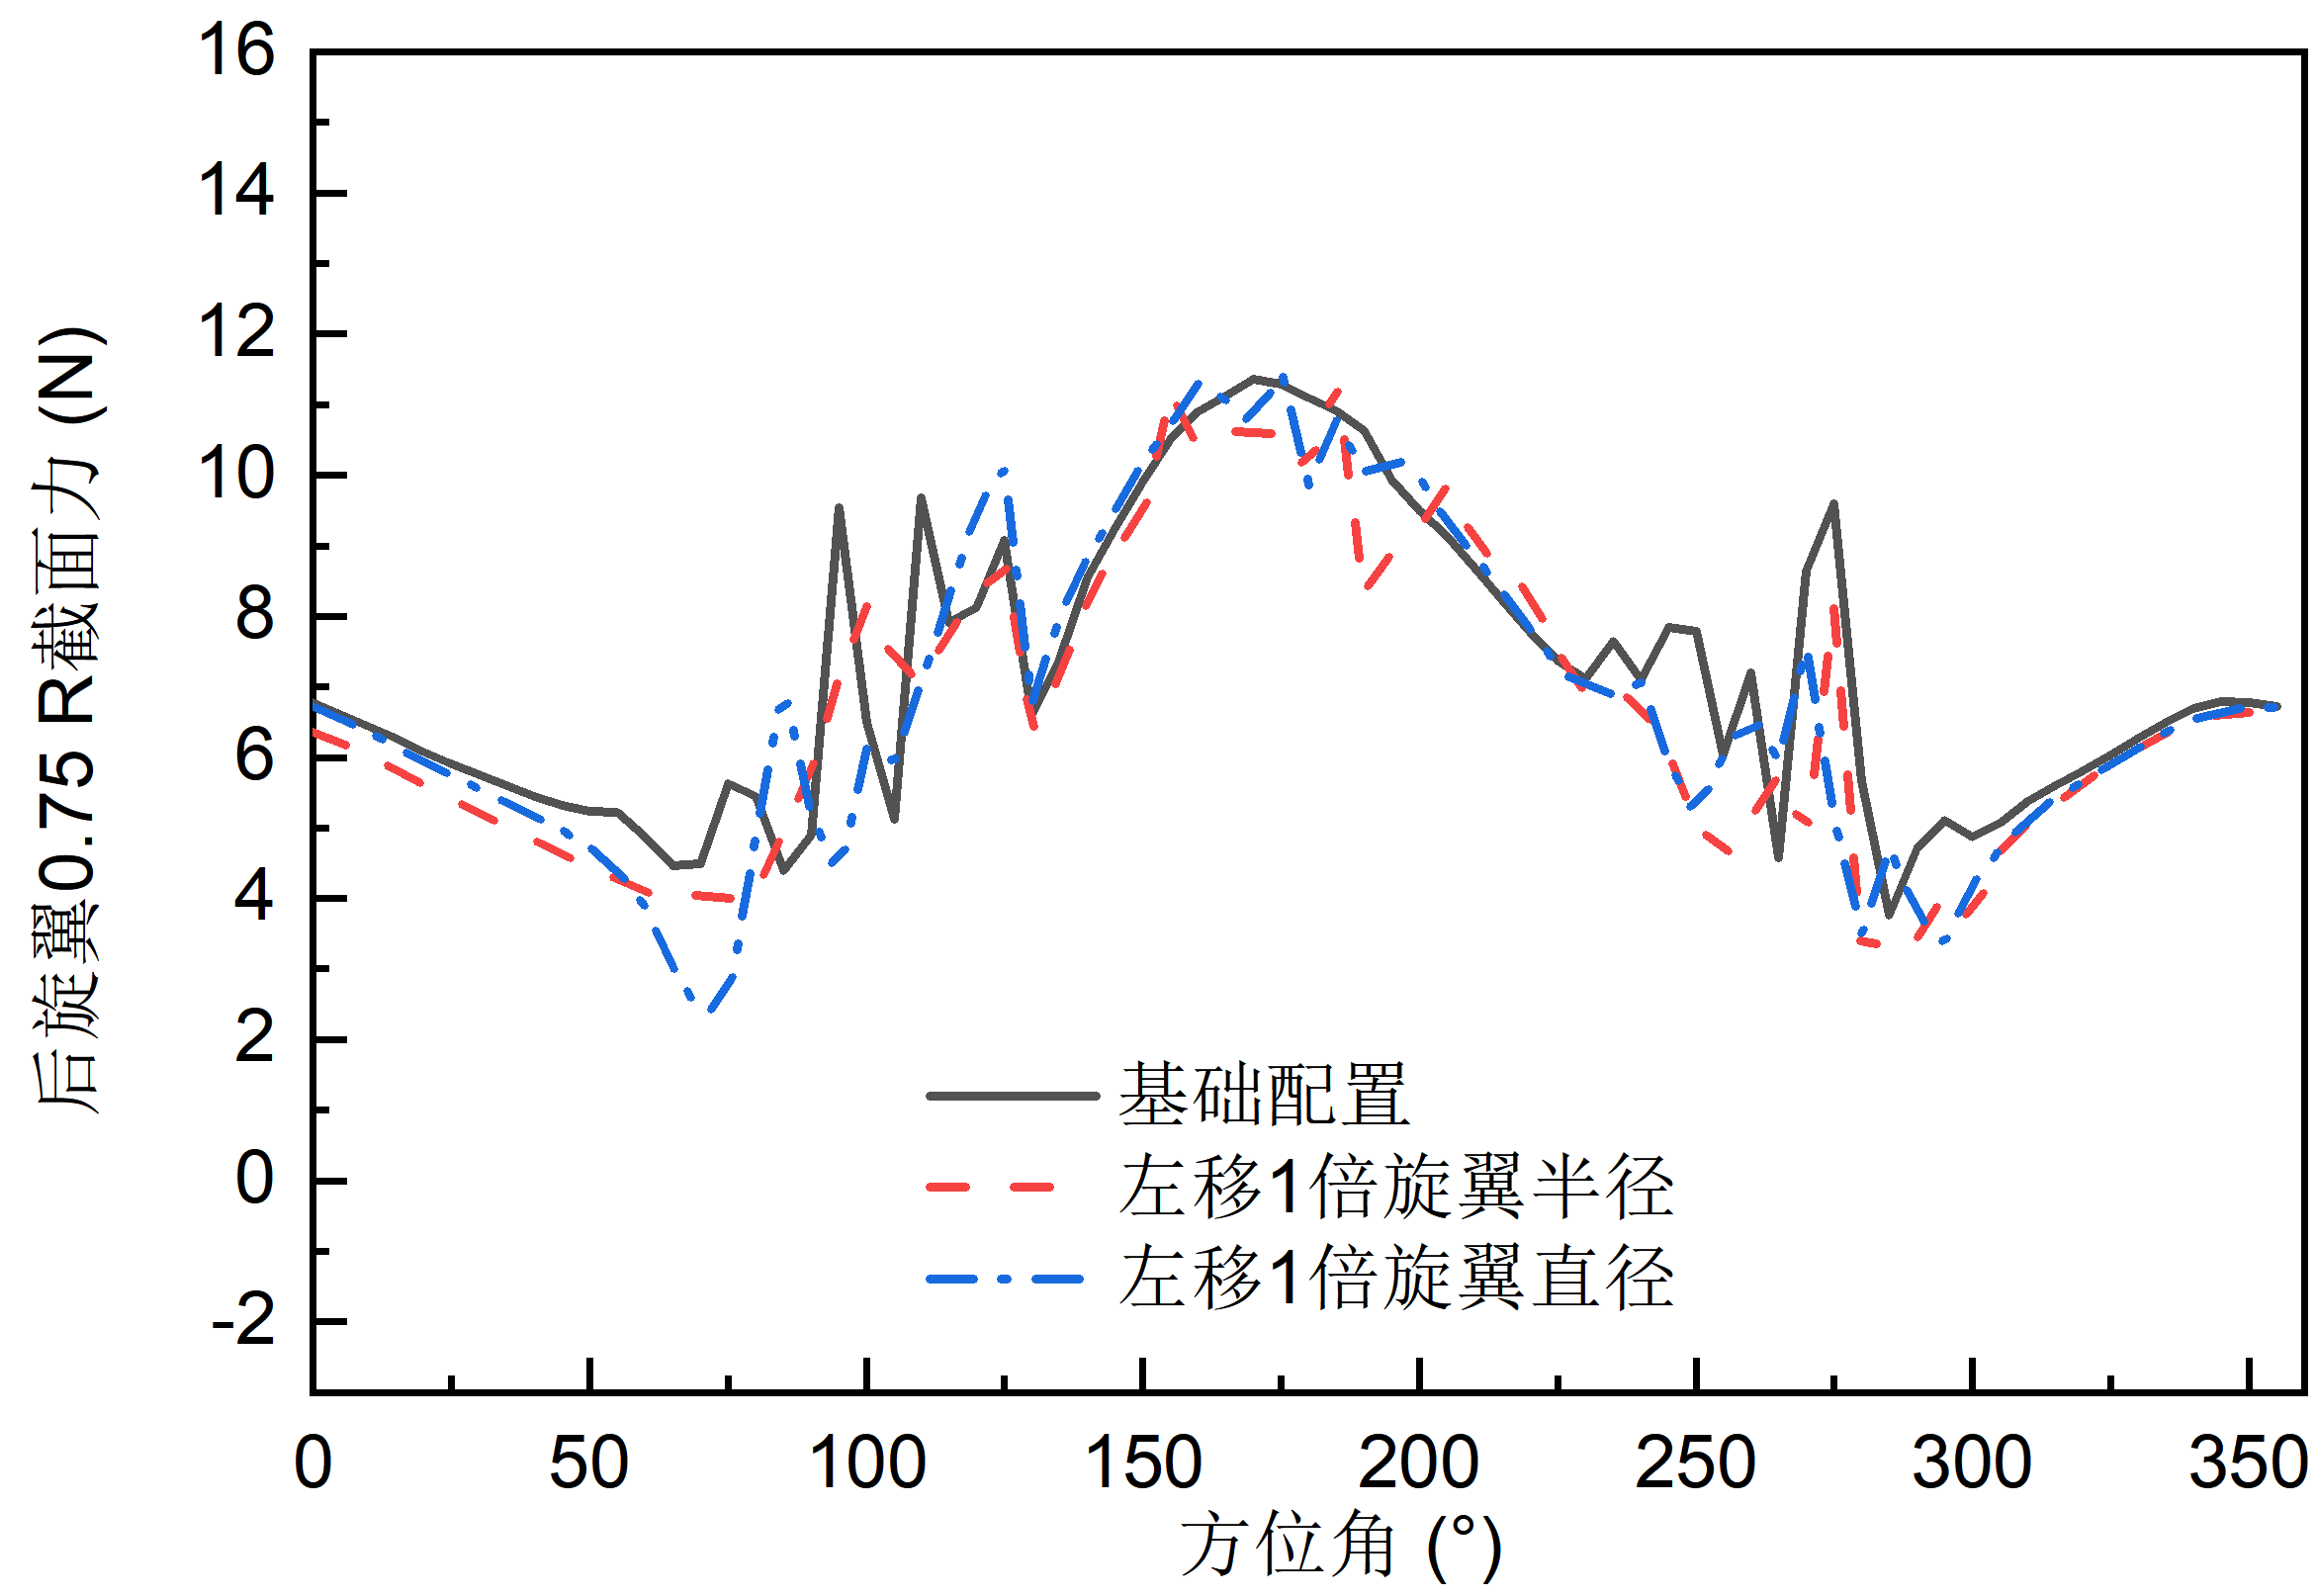
\includegraphics[width=7cm]{fig/figure_chap3/chap_3_5_2_5.png}}
  \caption{不同侧向相对位置下0.75 R 处的截面力}
  \label{fig:chap3_5_2_2}
\end{figure}

图\ref{fig:chap3_5_2_3}给出不同侧向相对位置下直升机1拉力和功率的变化。其中,100\%的前旋翼拉力对应95 N;100\%的后旋翼拉力对应83 N。100\%的前旋翼功率对应310 W;100\%的后旋翼功率对应452 W。这些值是直升机1不受直升机4的气动干扰影响时计算得到的。基本配置中,即相对侧向位置等于0时,前旋翼有20\%的拉力损失和15\%的功耗增加。随着侧向相对位置正向、负向增加,拉力增加、功耗减小。当侧向相对位置处于-1.5到-0.75倍的旋翼直径、0.75到1.5倍的旋翼直径时,相比无干扰时,拉力增加、功率减小。这得益于较小的下洗流干扰和卷起涡引起的迎角增加。此外,后旋翼拉力和功率的变化较小。这与横向相对位置变化时,后旋翼0.75 R 截面拉力的变化规律是一致的。

\begin{figure}[!htb]
  \centering
  \subfloat[拉力变化]{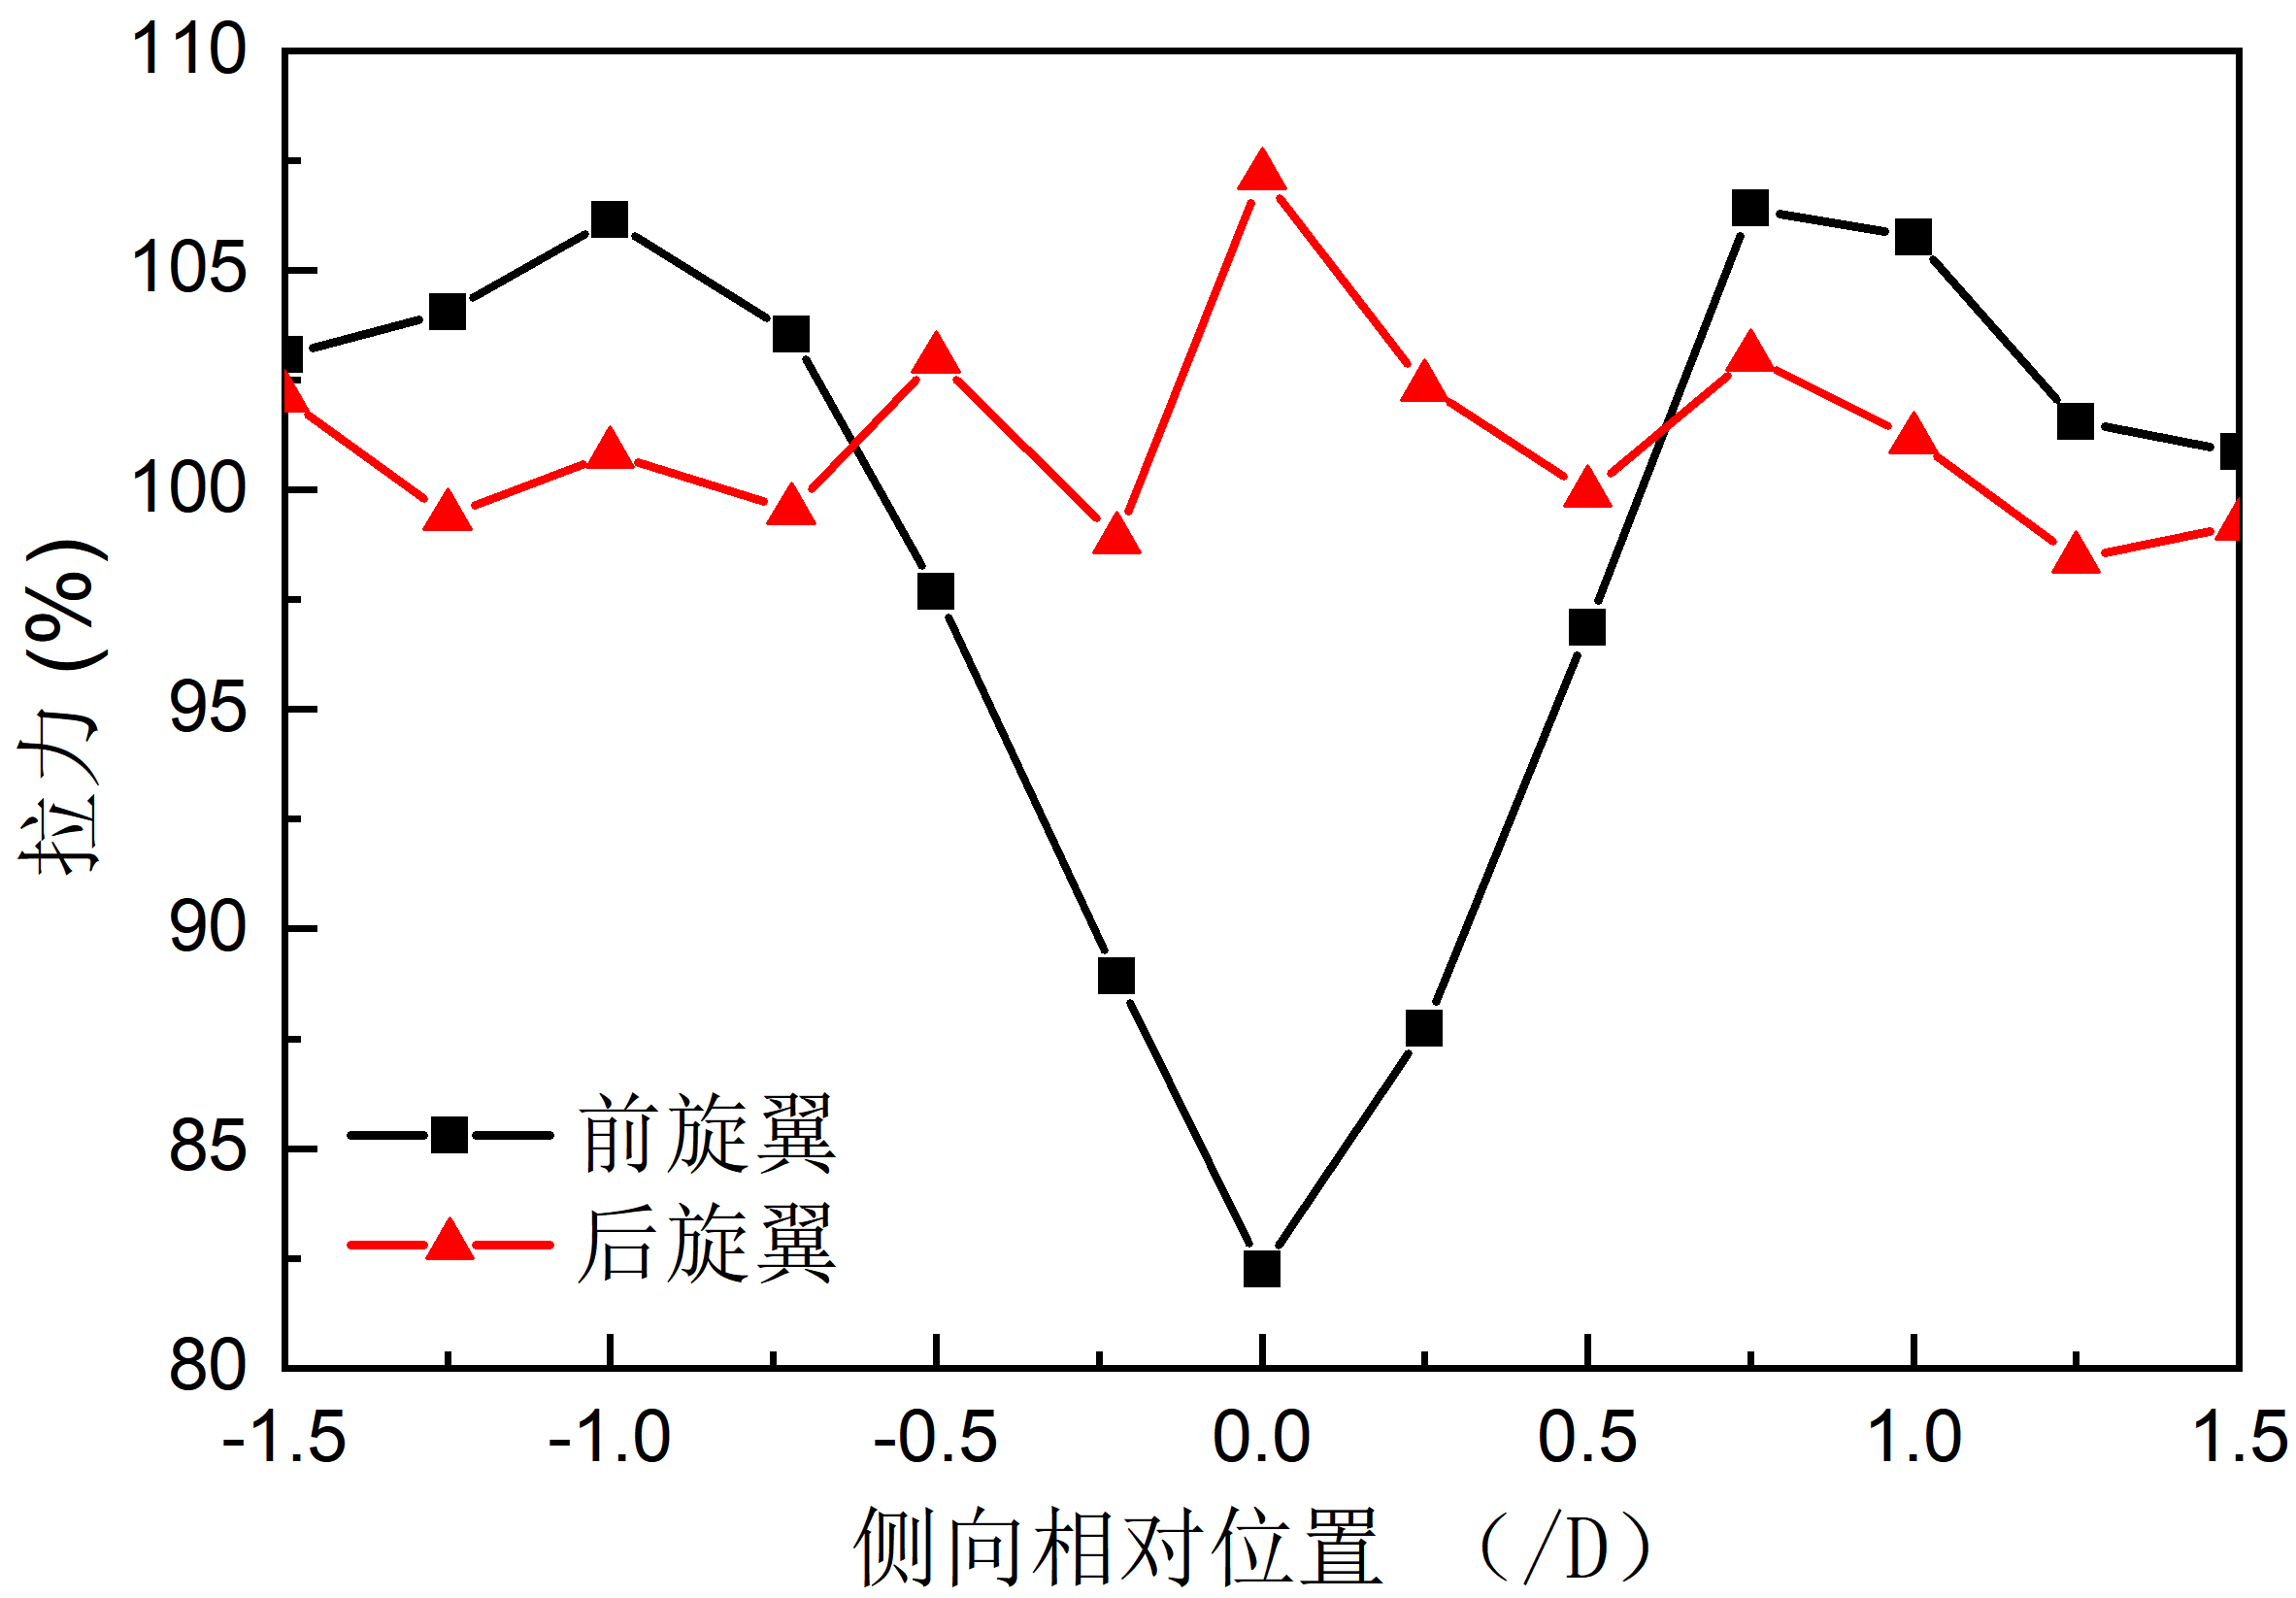
\includegraphics[width=7cm]{fig/figure_chap3/chap_3_5_2_6.png}}\quad 
  \subfloat[功率变化]{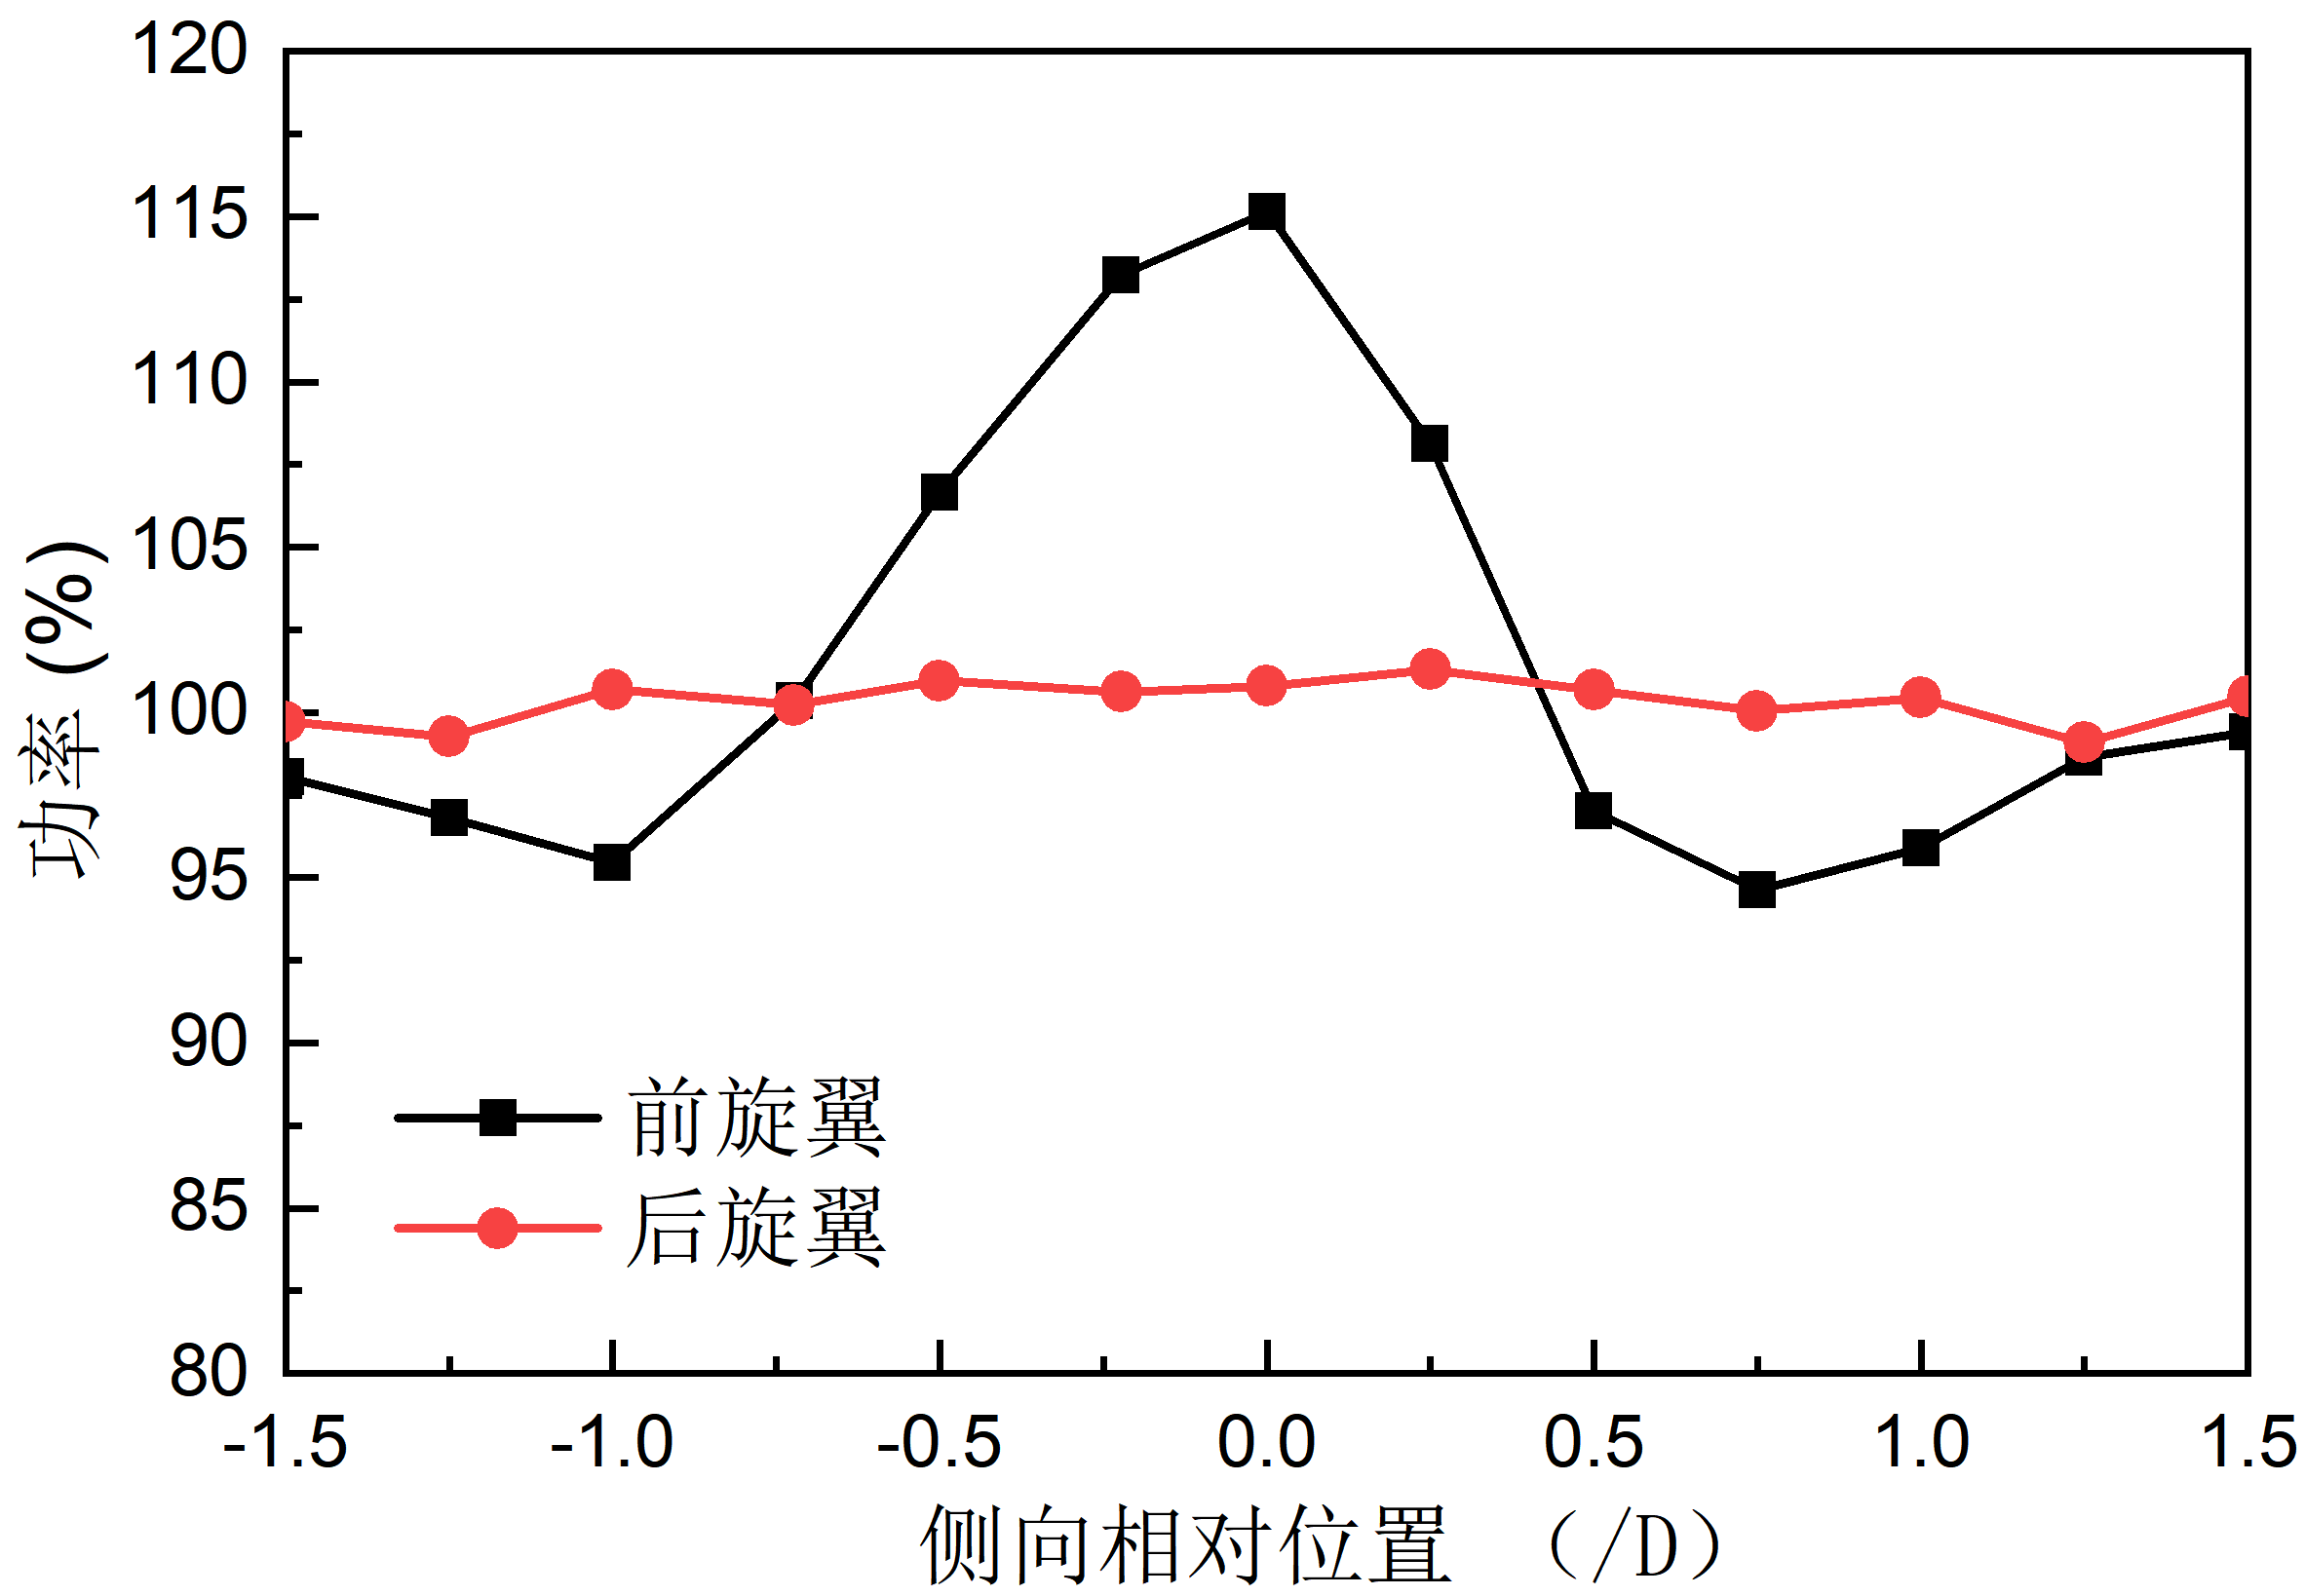
\includegraphics[width=7cm]{fig/figure_chap3/chap_3_5_2_7.png}}
  \caption{不同侧向相对位置下直升机1拉力和功率的变化}
  \label{fig:chap3_5_2_3}
\end{figure}

可见,基本配置中,由于气动干扰的影响直升机1有一定的拉力损失和功耗增加。通过合理调整直升机1相对直升机4的侧向位置,拉力损失和功率都会减小。甚至当侧向相对位置处于-1.5到-0.75倍的旋翼直径、0.75到1.5倍的旋翼直径时,相对无干扰时拉力增加、功效减小。
\subsection{不同纵向相对位置下气动干扰及性能的变化}
本小节给出了气动干扰随直升机纵向相对位置的变化。图\ref{fig:chap3_5_3_1}给出了直升机1相对基本配置前进、后退1个旋翼半径时的涡度场。与基本配置中的涡度场(见图\ref{fig:chap3_5_2_1}(a))相比可以发现,气动干扰随着直升机1和直升机4间距离的减小而增加。
\begin{figure}[!htb]
  \centering
  \subfloat[直升机1向前1个旋翼半径]{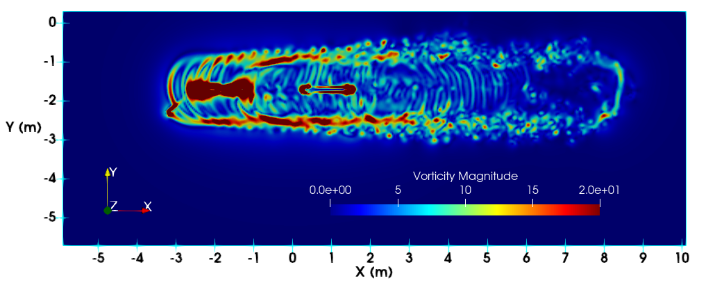
\includegraphics[width=7cm]{fig/figure_chap3/chap_3_5_3_1.png}}\quad 
  \subfloat[直升机1向后1个旋翼半径]{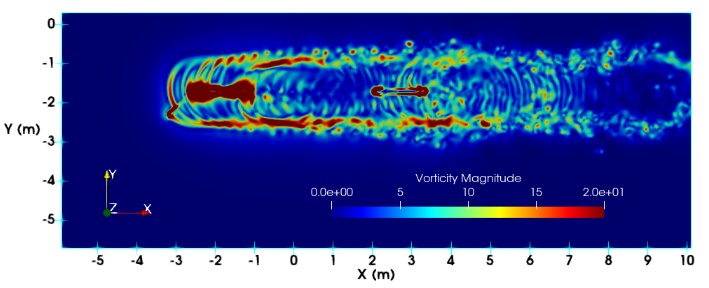
\includegraphics[width=7cm]{fig/figure_chap3/chap_3_5_3_2.png}}
  \caption{直升机协同吊挂系统不同纵向相对位置下的涡度场}
  \label{fig:chap3_5_3_1}
\end{figure}

图\ref{fig:chap3_5_3_2}给出了前后旋翼不同纵向相对位置下0.75 R 处的截面力。从图\ref{fig:chap3_5_3_2}(a)可以看出,多数方位角下直升机1后退1倍旋翼半径时其前旋翼的截面力均大于其他两种情况。这与上面提到的气动干扰的变化一致。与不同侧向相对位置时的结果相似,三种情况下后旋翼截面力的变化较小。这也导致了后旋翼合力、功率变化较小,分别见图\ref{fig:chap3_5_3_3}(b)和图\ref{fig:chap3_5_3_4}(b)。
\begin{figure}[!htb]
  \centering
  \subfloat[前旋翼]{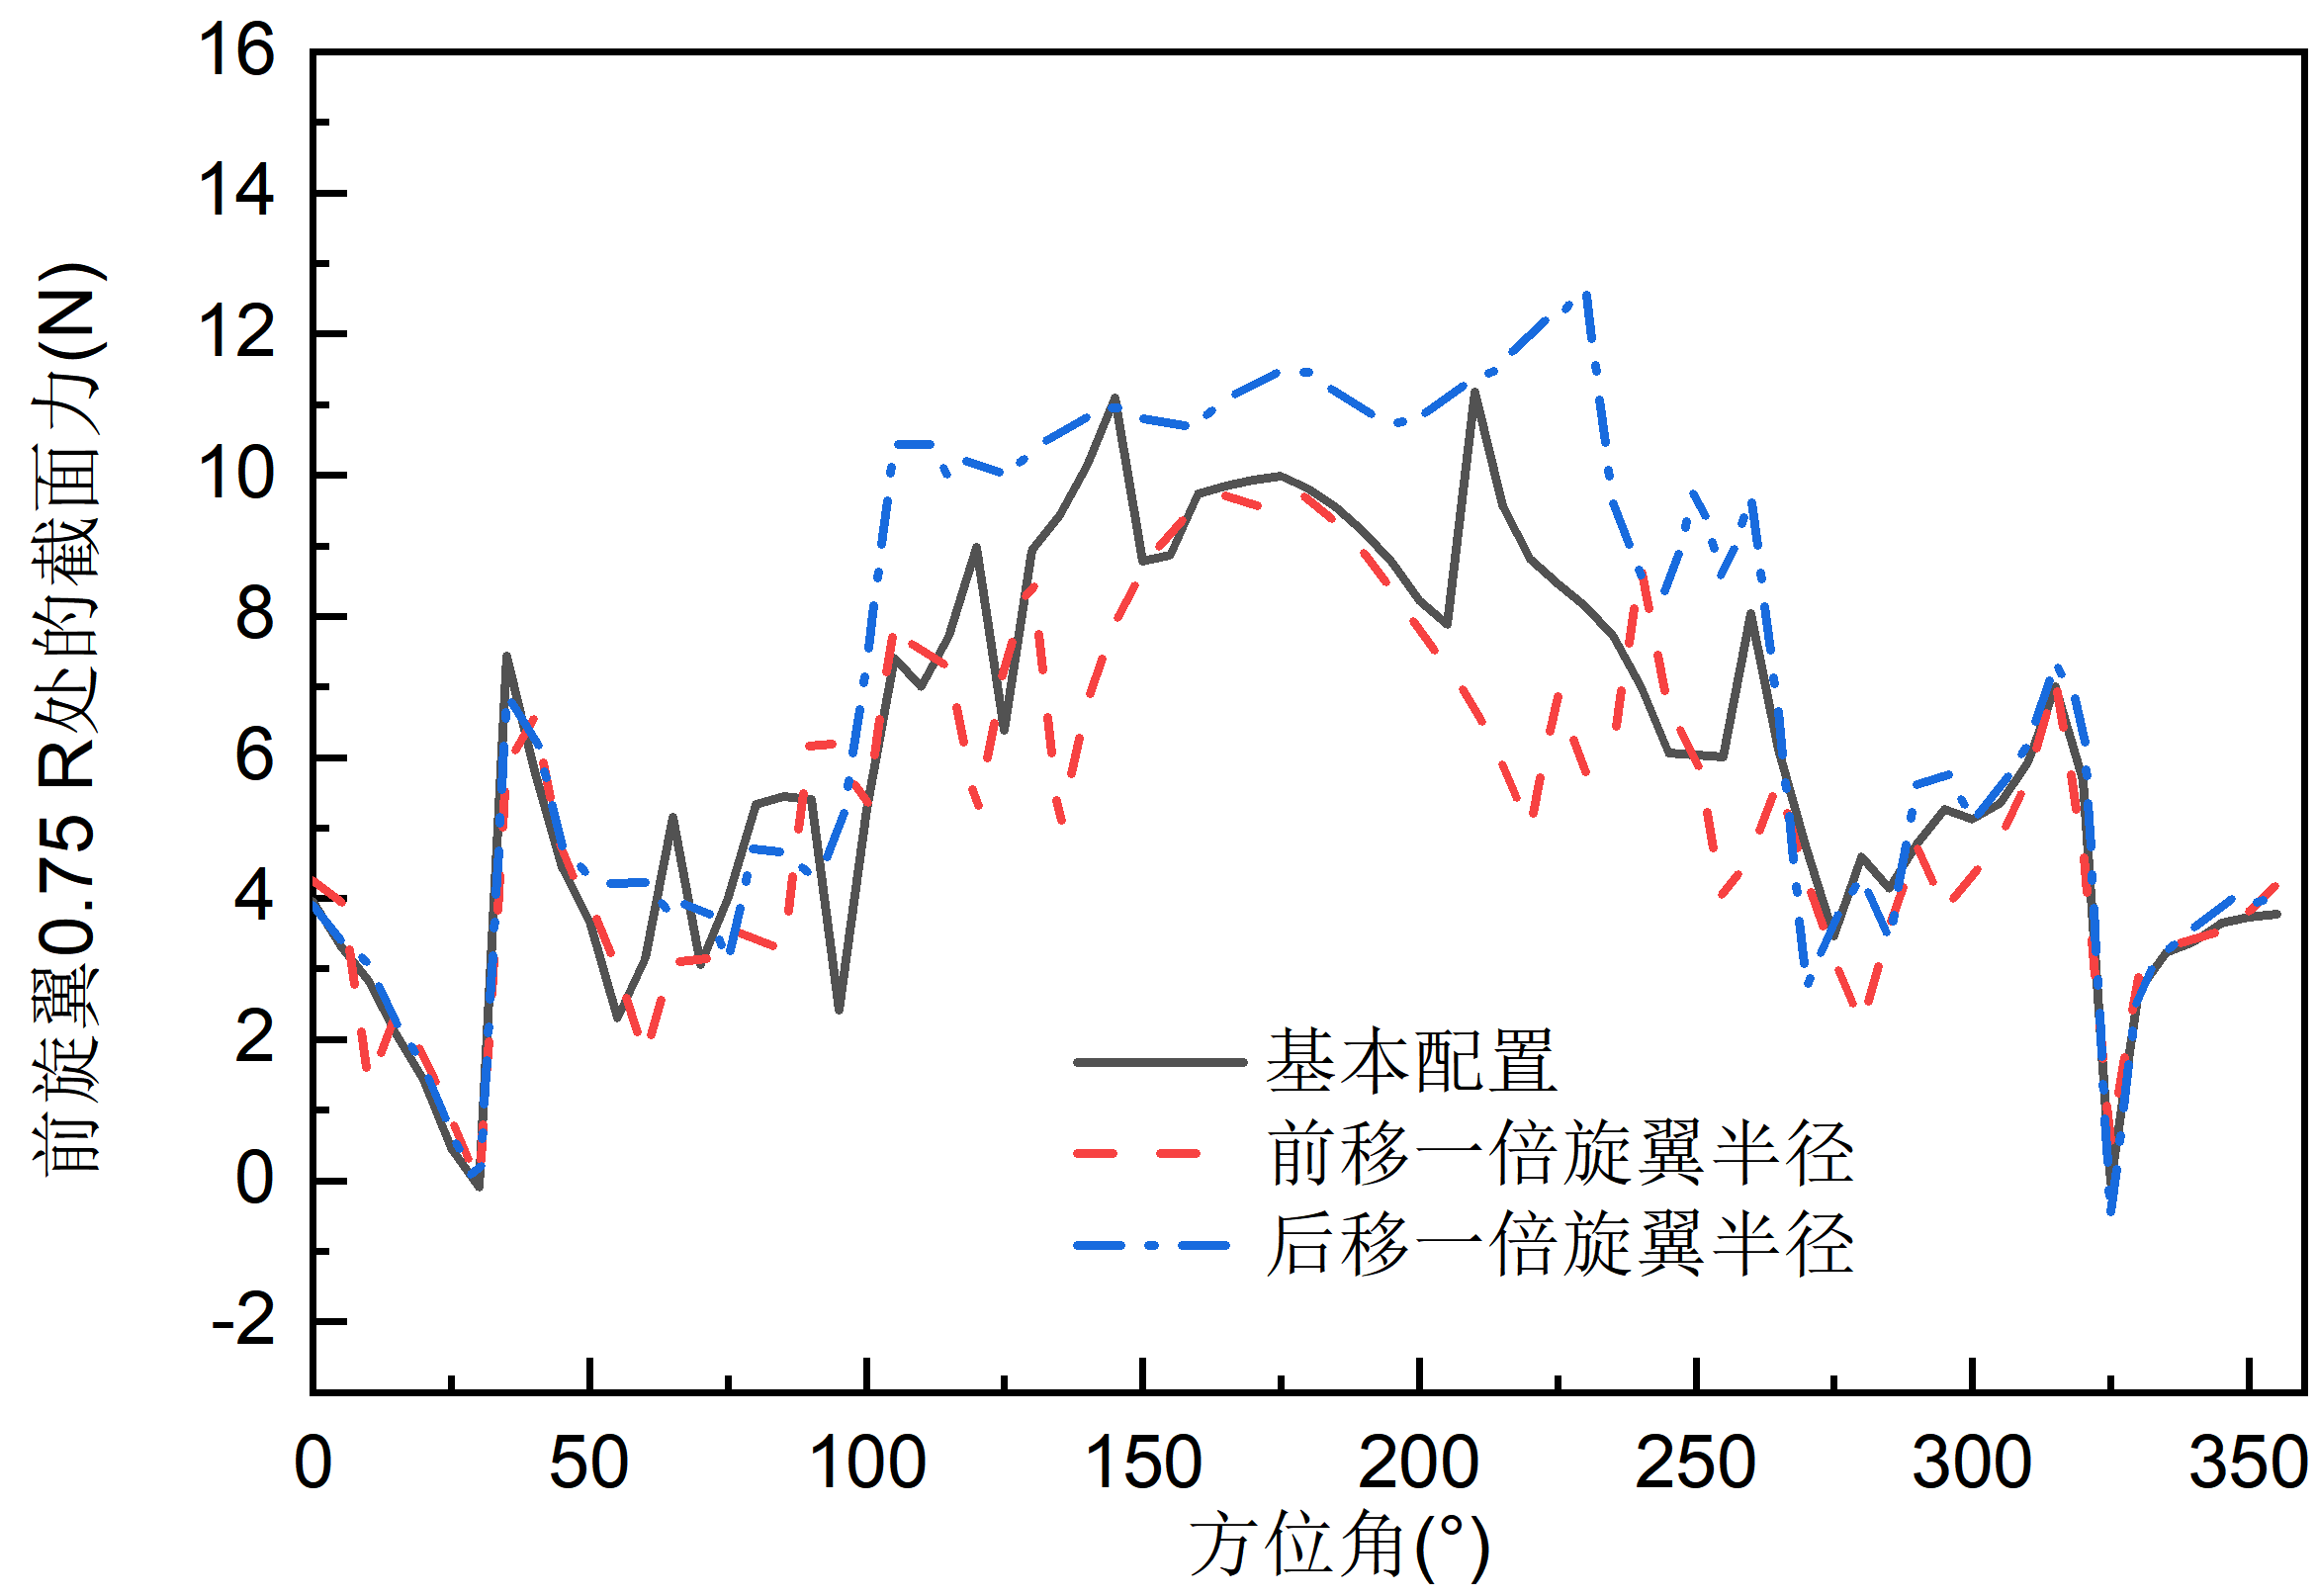
\includegraphics[width=7cm]{fig/figure_chap3/chap_3_5_3_3.png}}\quad
  \subfloat[后旋翼]{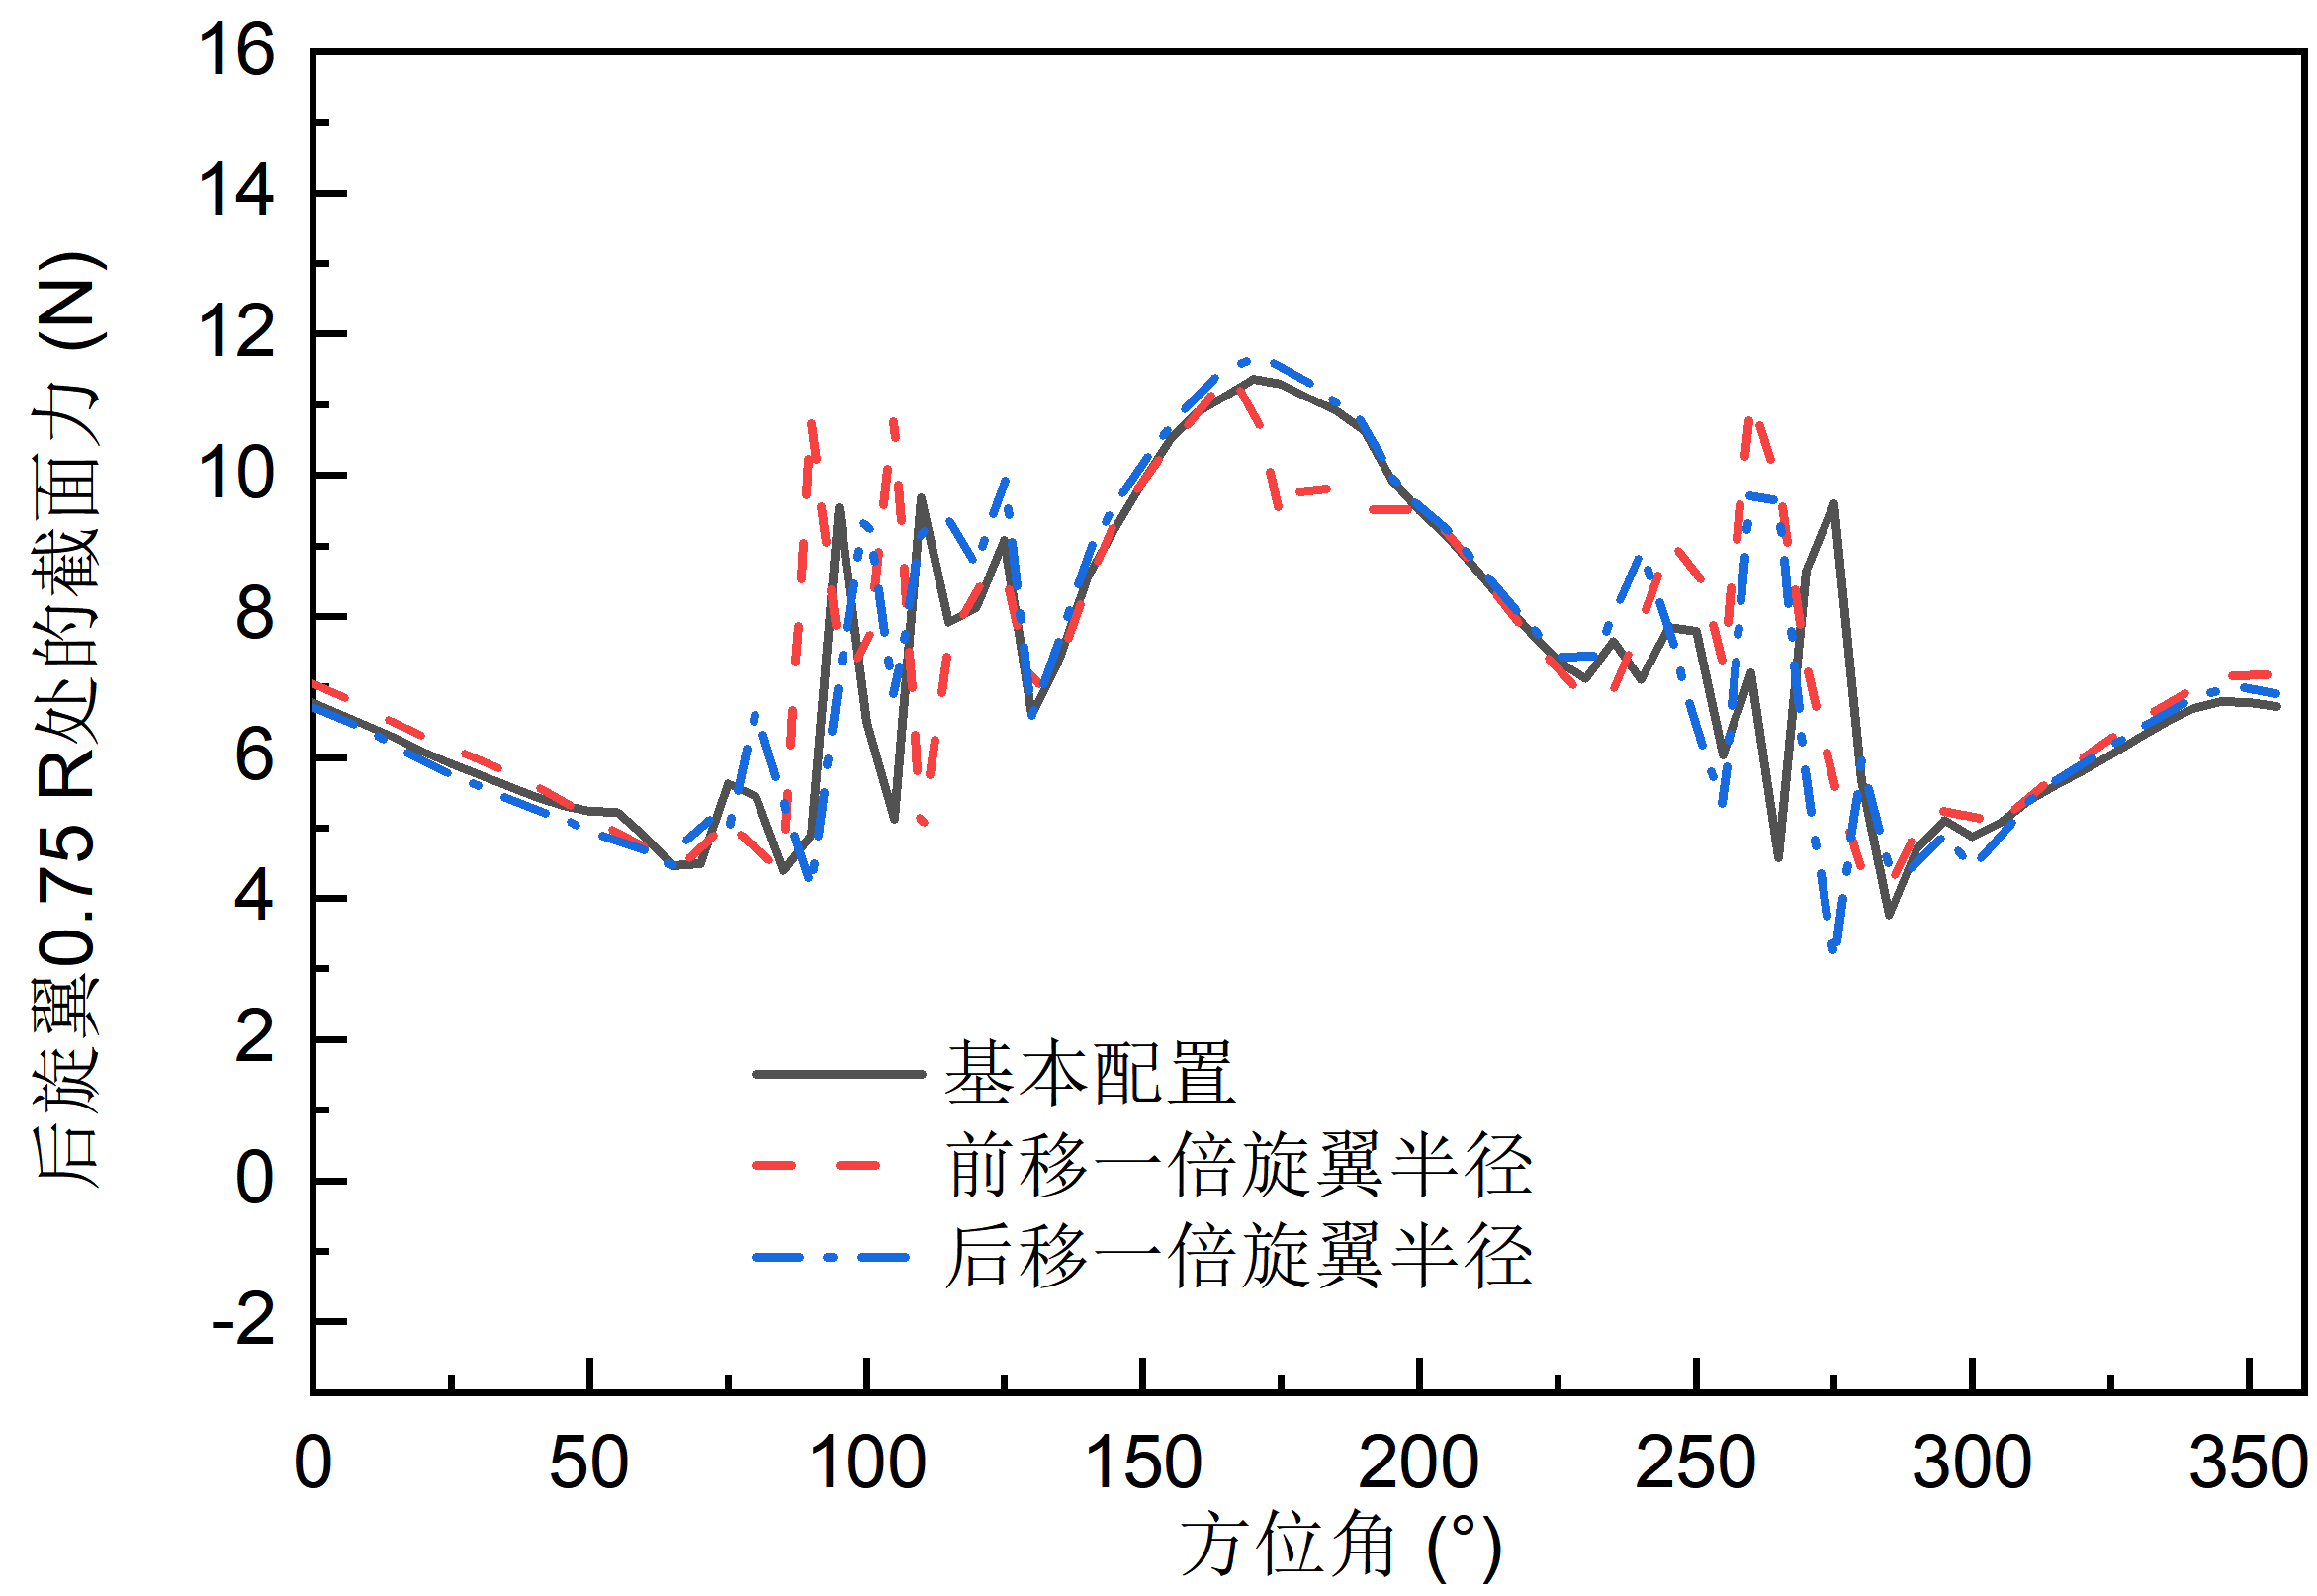
\includegraphics[width=7cm]{fig/figure_chap3/chap_3_5_3_4.png}}
  \caption{不同纵向相对位置下0.75 R 处的截面力}
  \label{fig:chap3_5_3_2}
\end{figure}

图\ref{fig:chap3_5_3_3}(a)和图\ref{fig:chap3_5_3_4}(a)给出了不同纵向相对位置下前旋翼拉力和功率的变化。可以看出,当侧向相对位置处于-1到1倍的旋翼半径时,拉力损失和功率消耗随着直升机1和直升机4间纵向相对位置的增加而减小。当侧向相对位置处于-1.5倍旋翼直径到-1倍旋翼半径、1倍旋翼半径到1.5倍旋翼直径时,拉力损失和功率消耗随着纵向相对距离的增加而增加。这是由于纵向相对距离越小,由上卷涡引起的作用在叶片上的上洗气流越大。

\begin{figure}[!htb]
  \centering
  \subfloat[前旋翼]{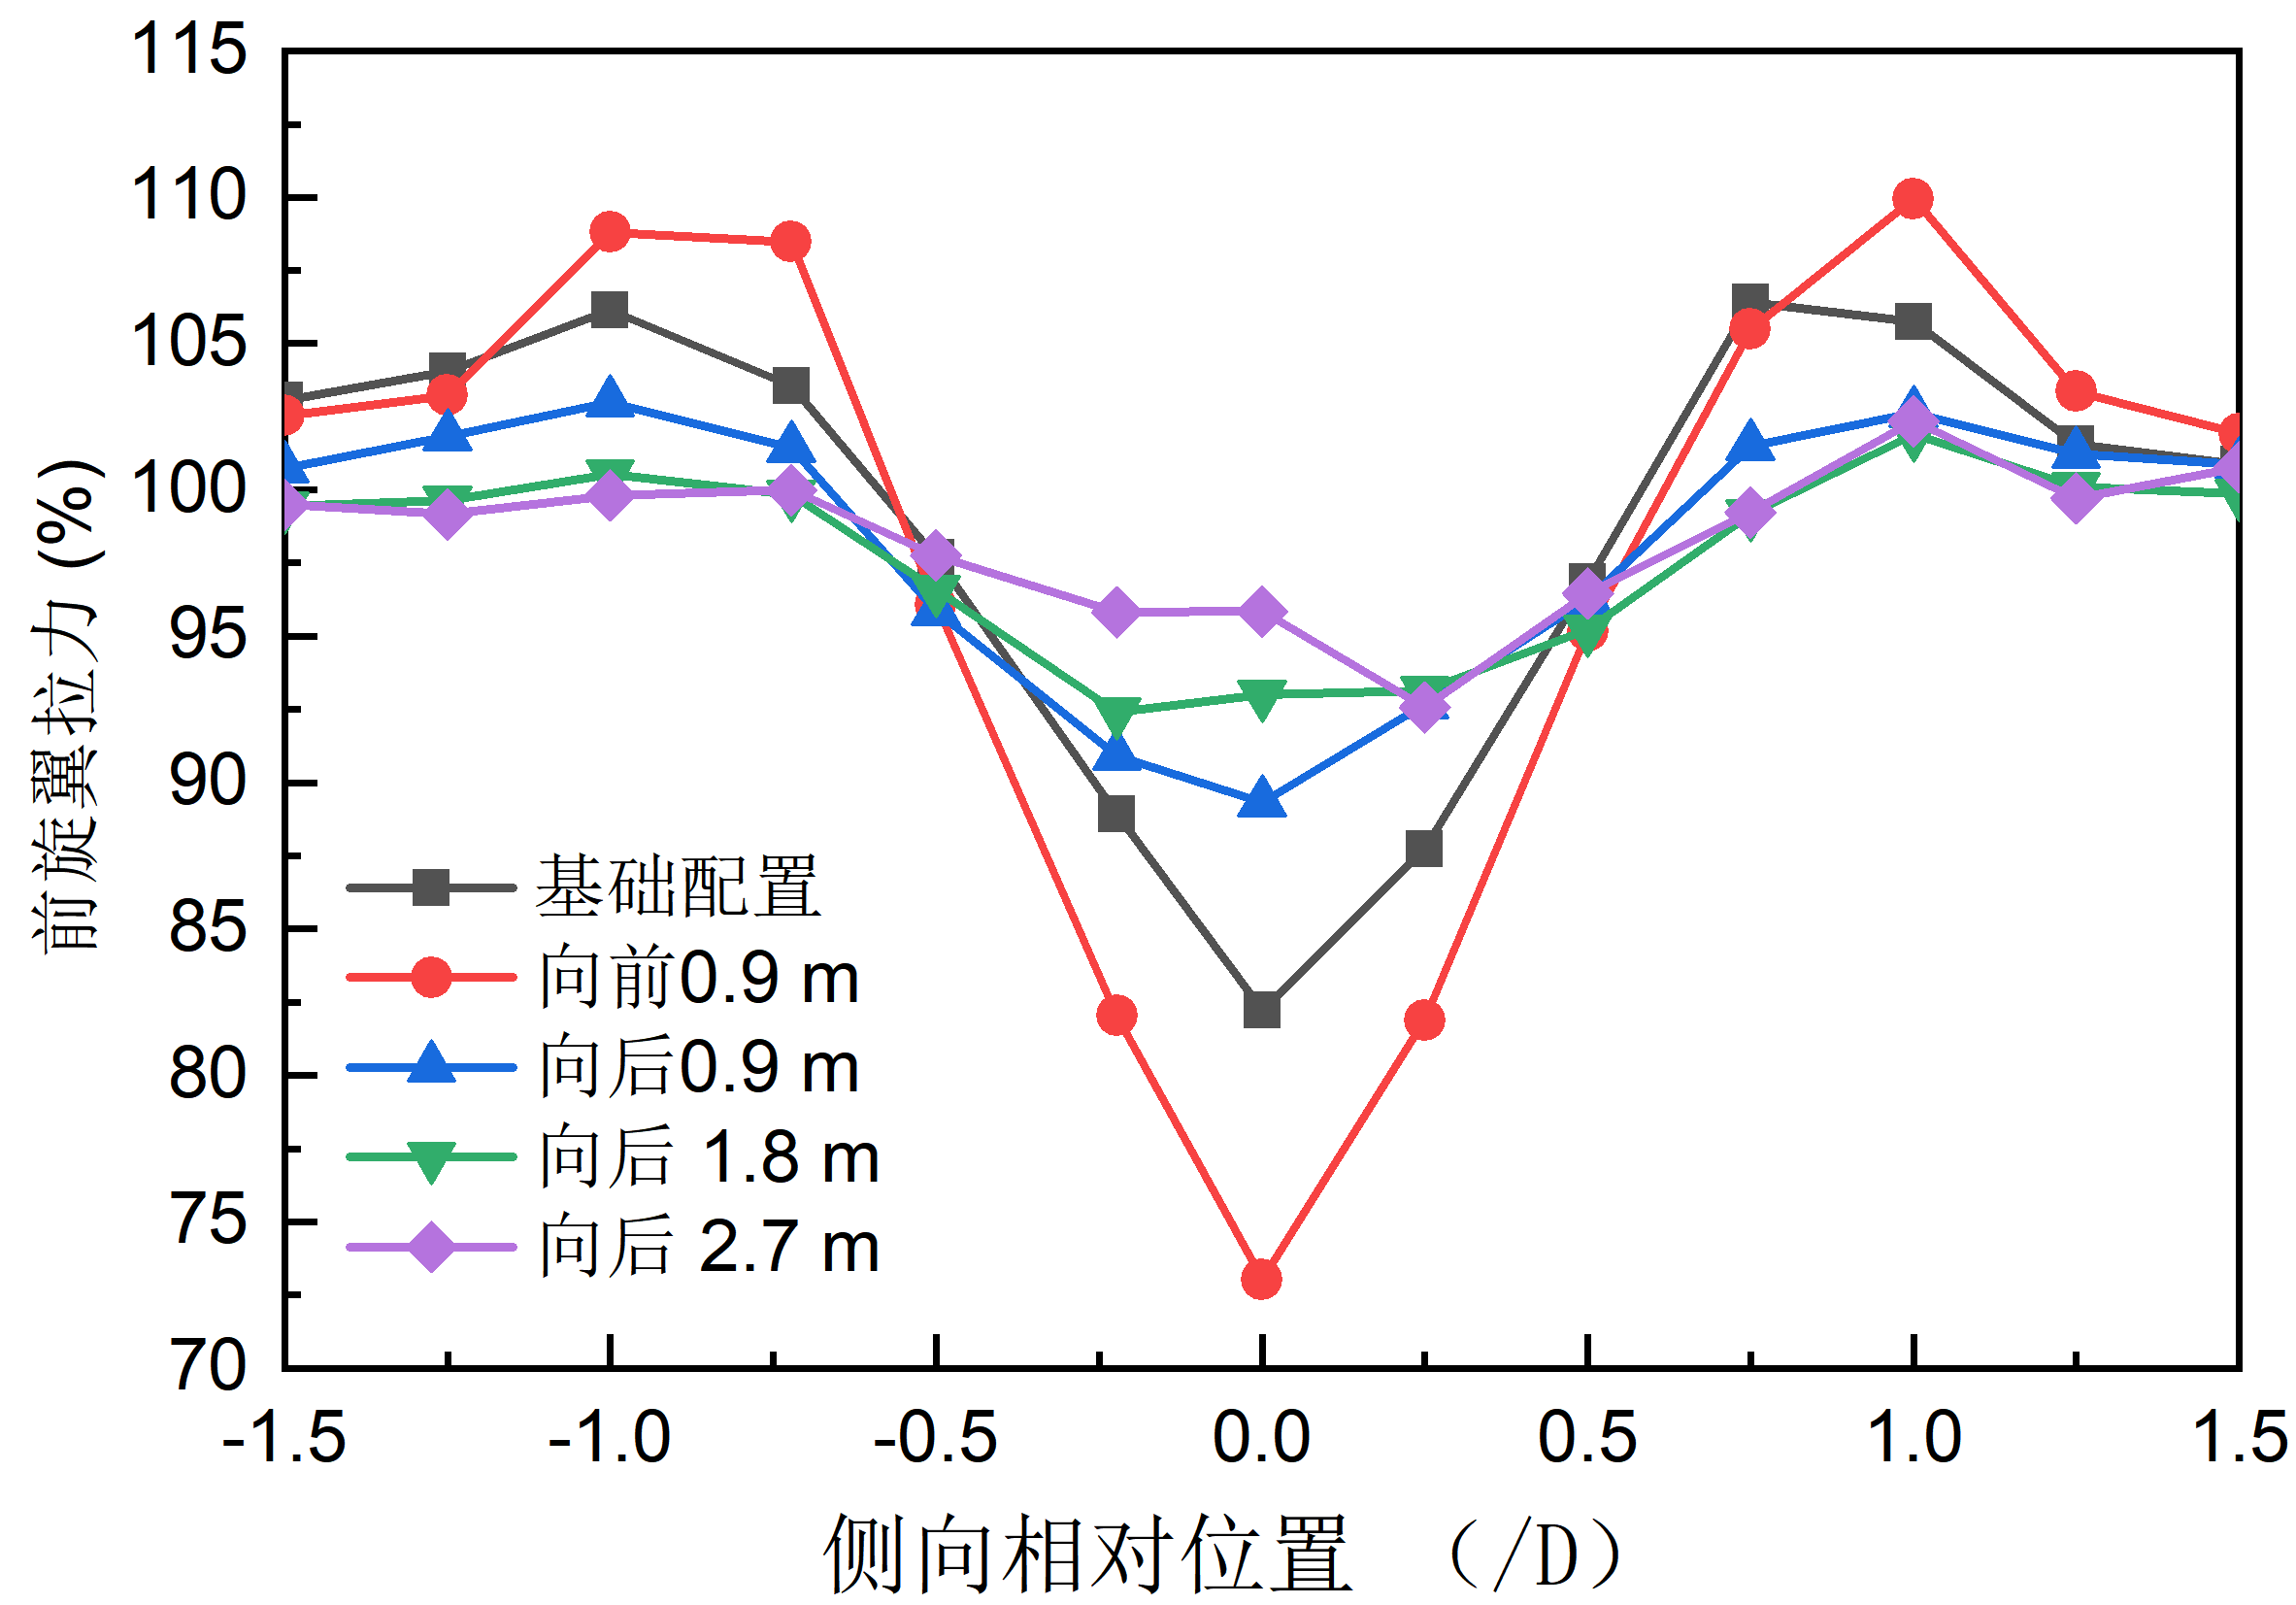
\includegraphics[width=7cm]{fig/figure_chap3/chap_3_5_3_5.png}}\quad
  \subfloat[后旋翼]{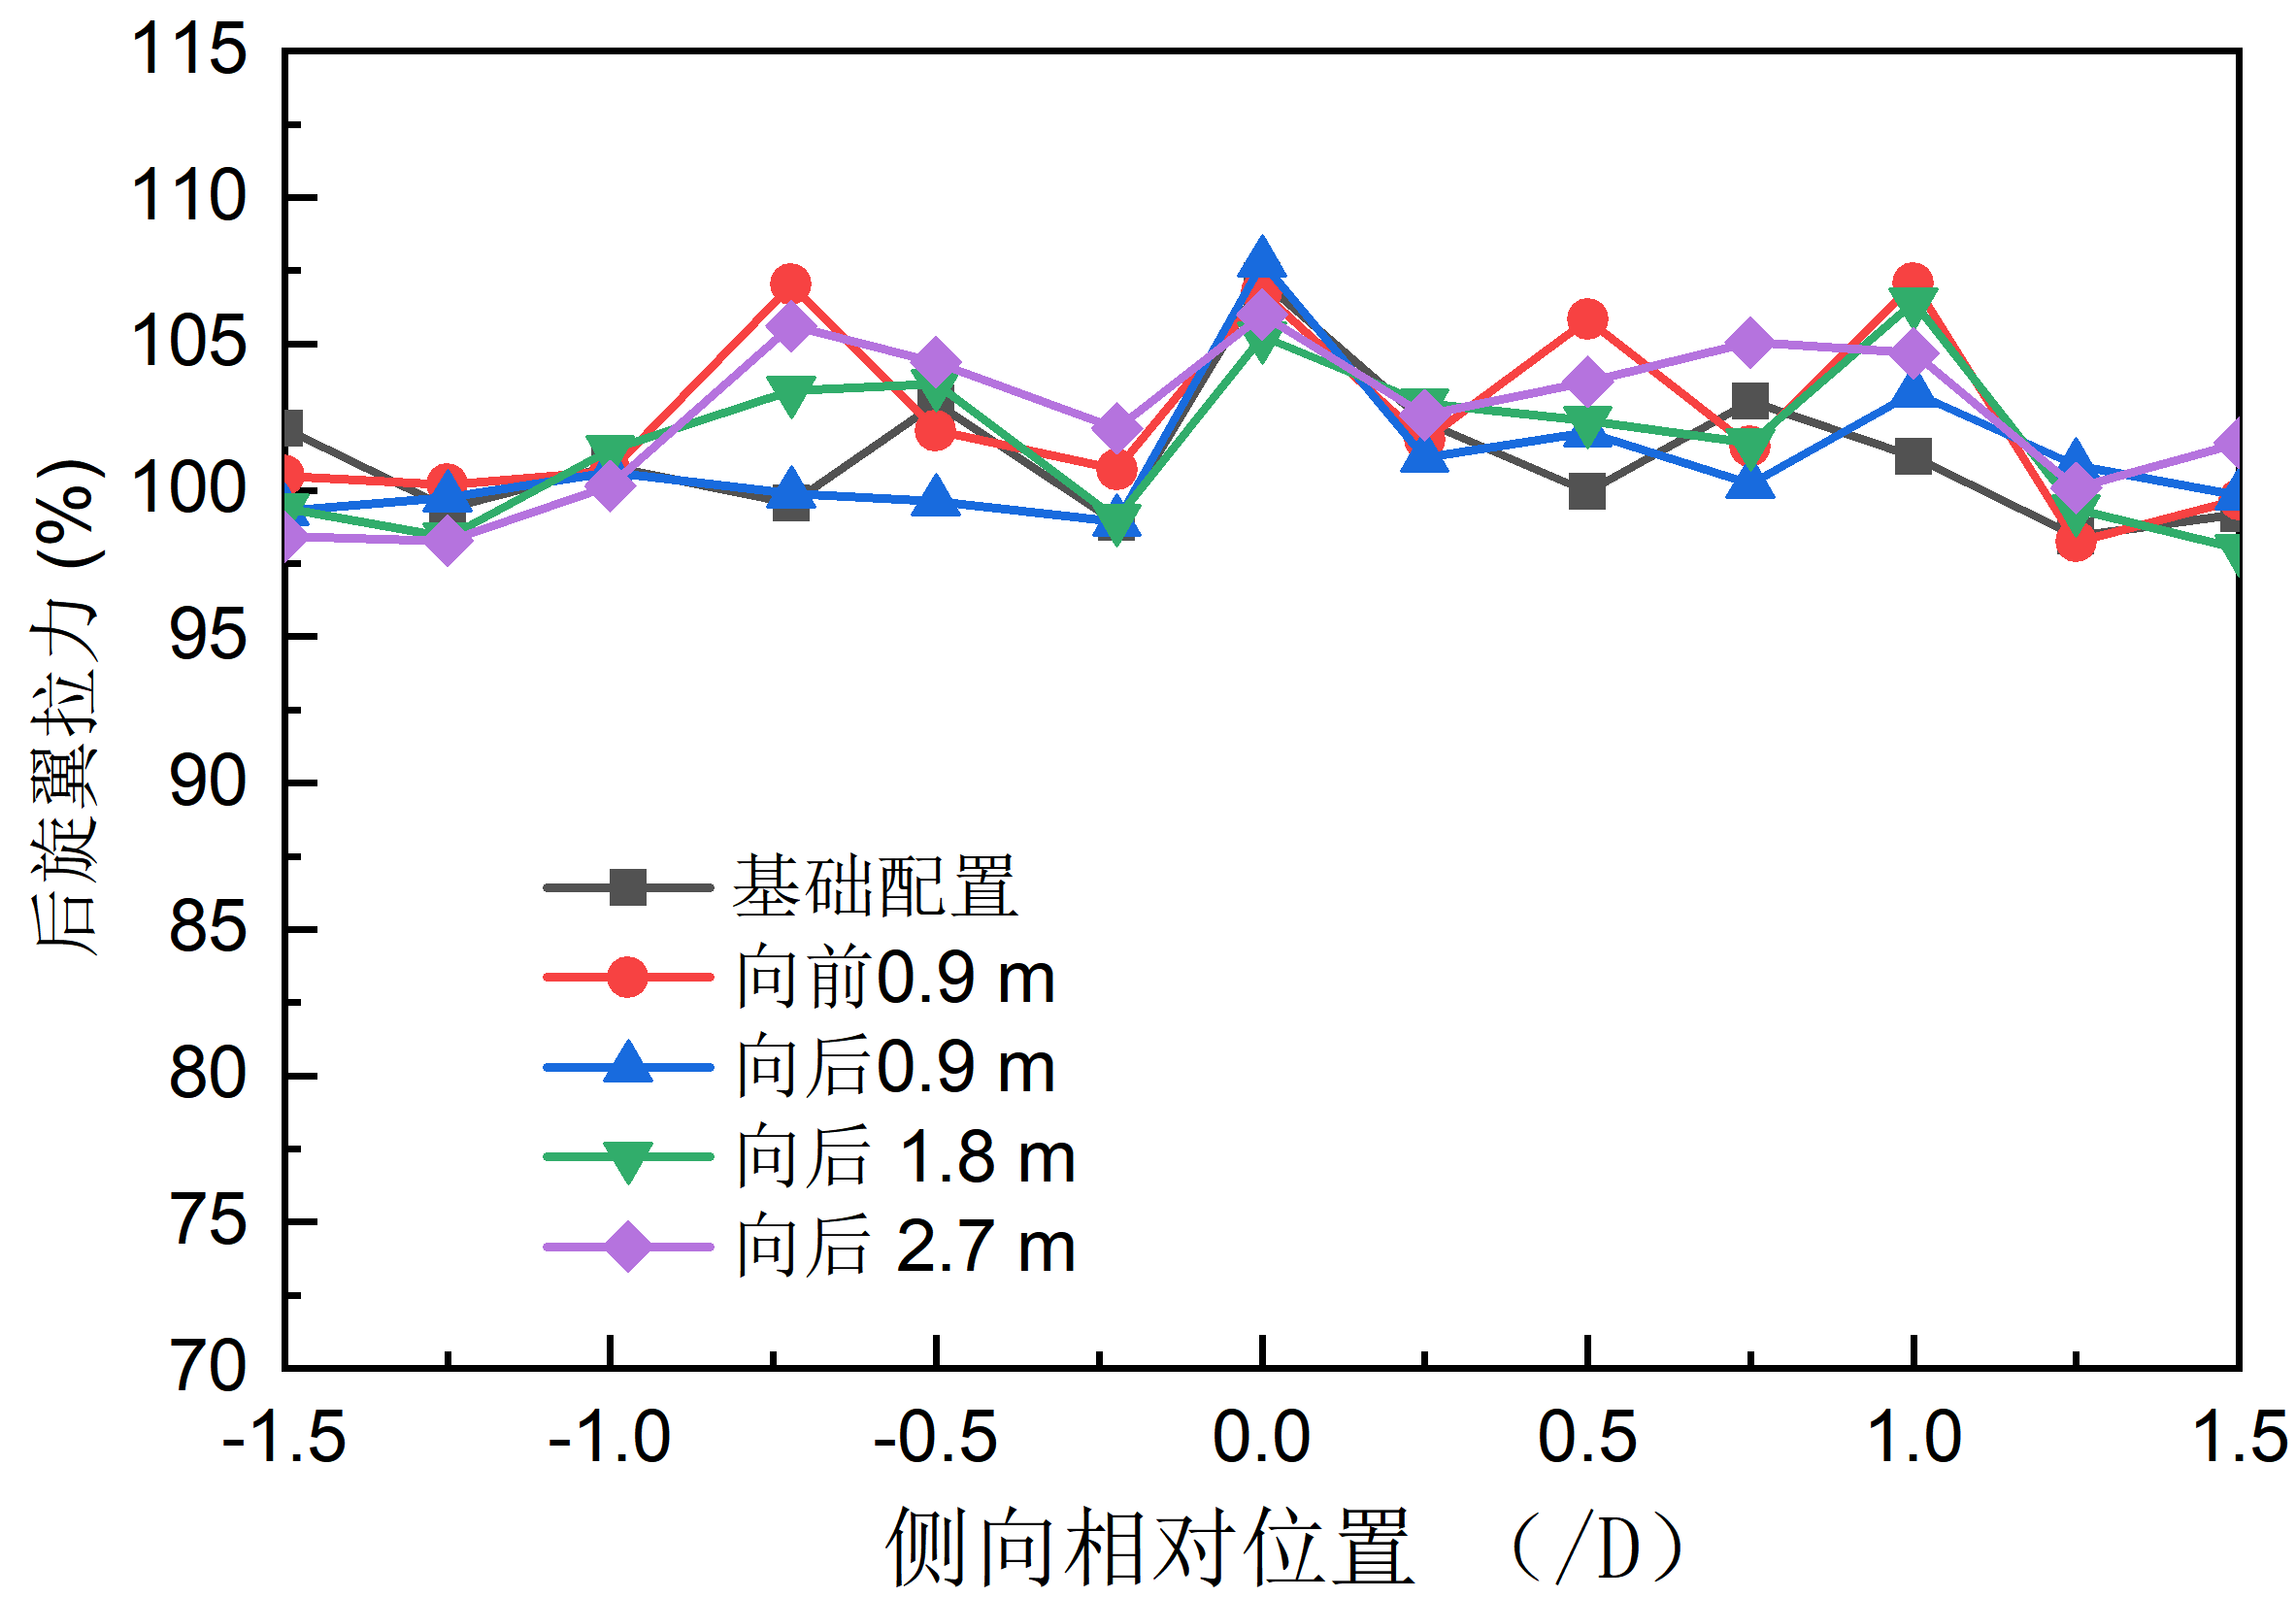
\includegraphics[width=7cm]{fig/figure_chap3/chap_3_5_3_6.png}}
  \caption{不同纵向相对位置下的旋翼拉力}
  \label{fig:chap3_5_3_3}
\end{figure}

\begin{figure}[!htb]
  \centering
  \subfloat[前旋翼]{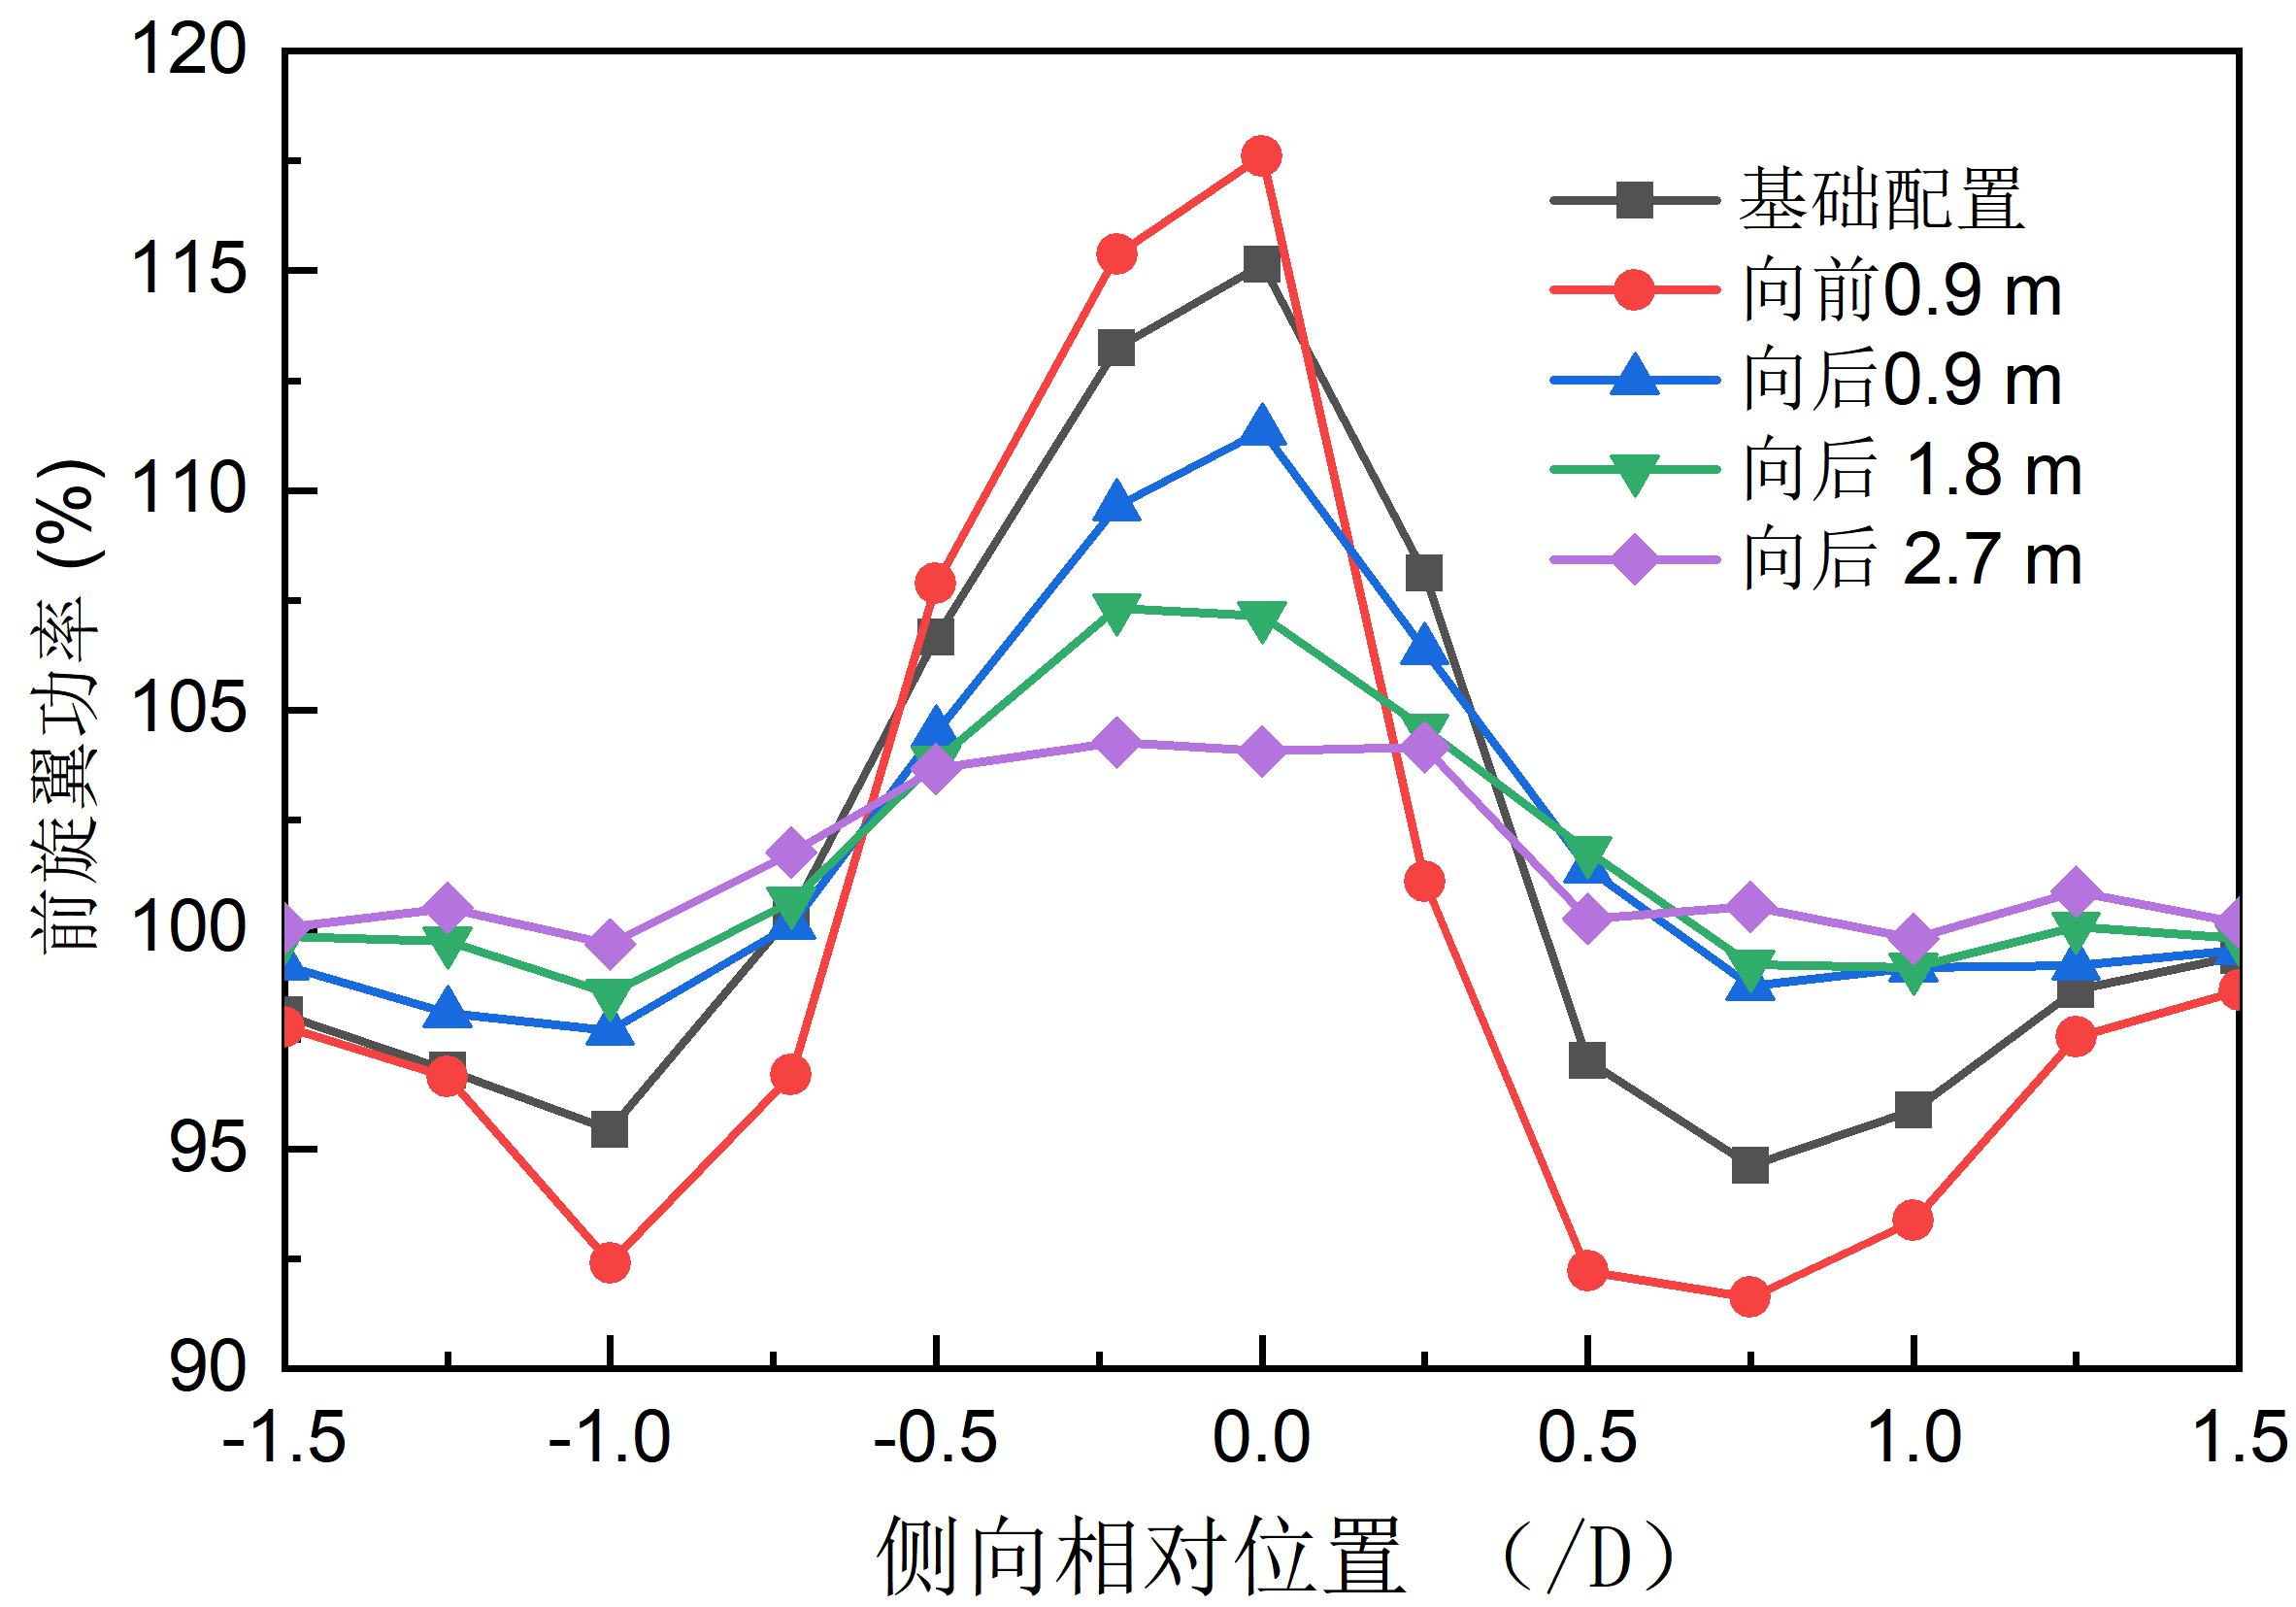
\includegraphics[width=7cm]{fig/figure_chap3/chap_3_5_3_7.png}}\quad
  \subfloat[后旋翼]{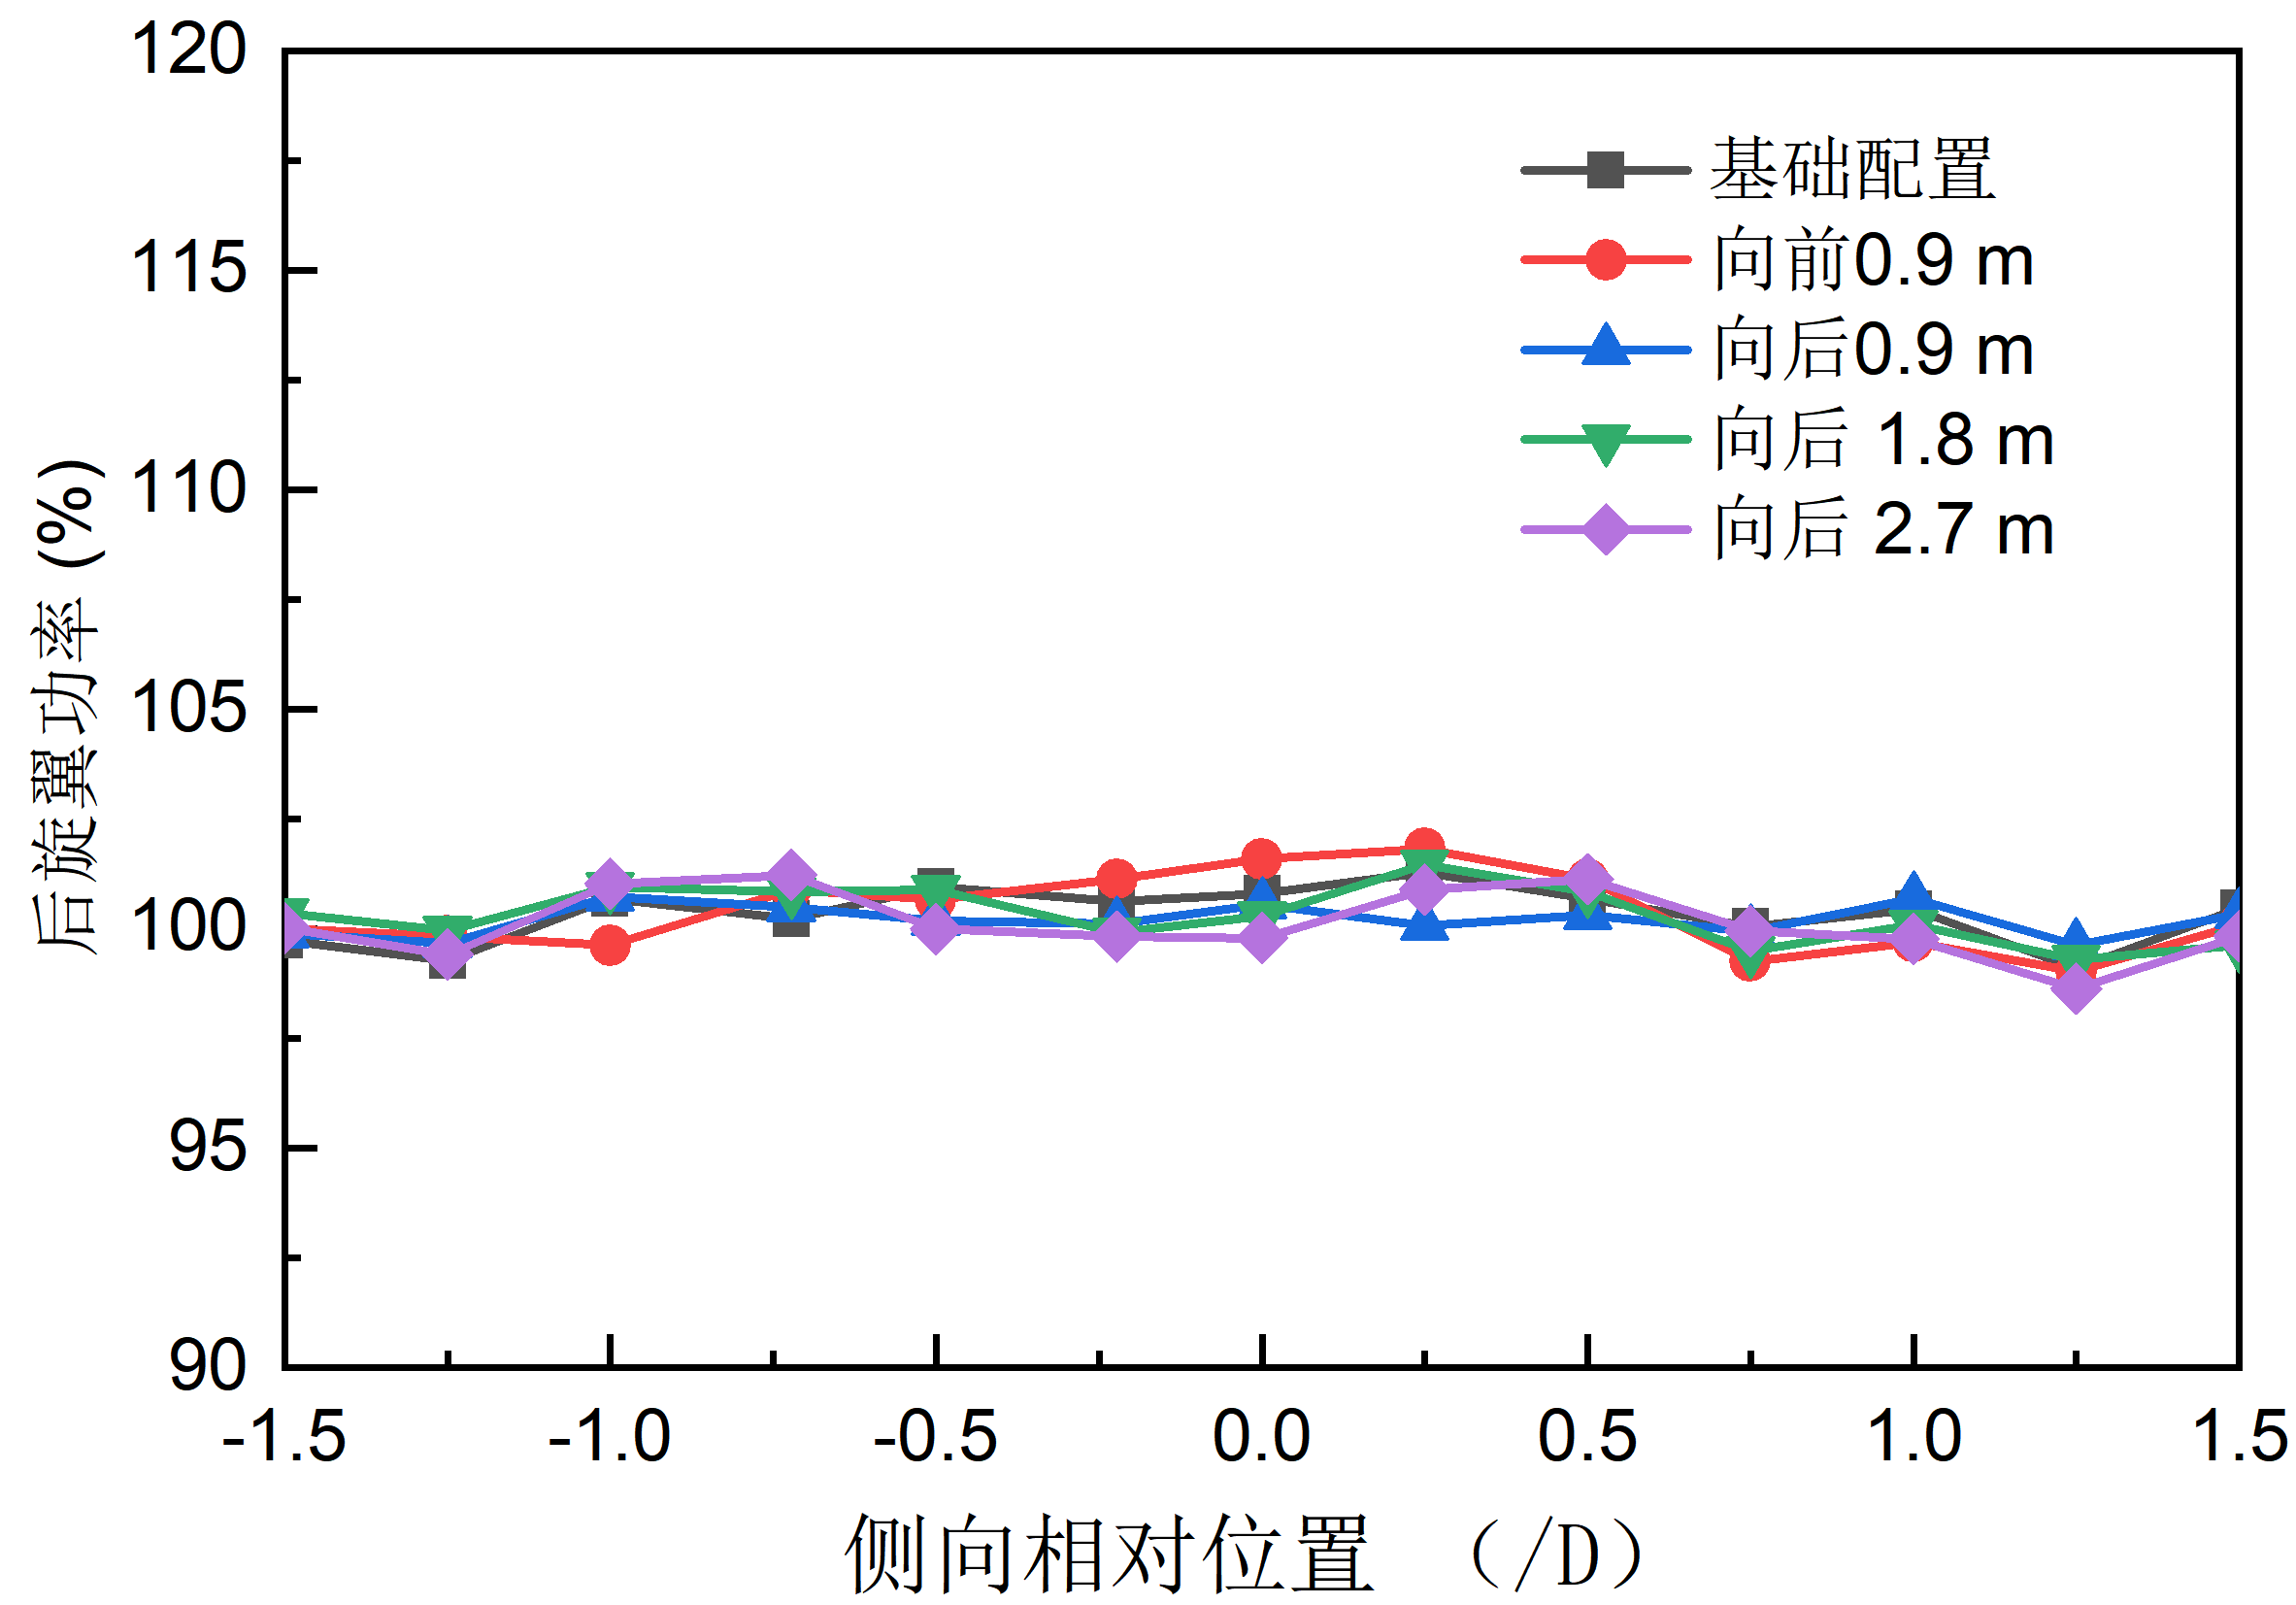
\includegraphics[width=7cm]{fig/figure_chap3/chap_3_5_3_8.png}}
  \caption{不同纵向相对位置下的旋翼功率}
  \label{fig:chap3_5_3_4}
\end{figure}
\subsection{不同垂向相对位置下气动干扰及性能的变化}
图\ref{fig:chap3_5_4_1}给出了直升机协同吊挂系统不同垂向相对位置下的涡度场。可以看出,在基础配置中直升机1的前半部分沉浸在直升机4的尾流中。当直升机1上移0.7 m后,直升机1和直升机4间几乎没有气动干扰。当直升机1下移0.7 m后,直升机1完全沉浸在直升机4的尾流中。
\begin{figure}[!htb]
  \centering
  \subfloat[基本配置]{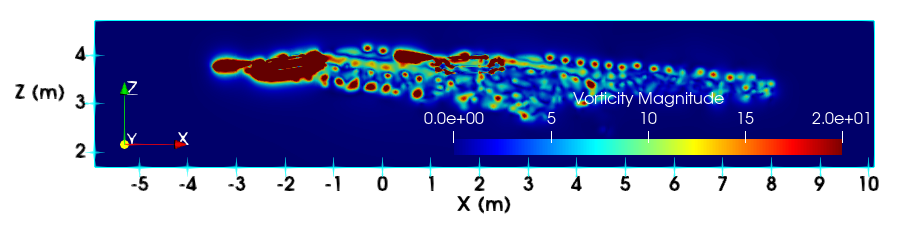
\includegraphics[width=7cm]{fig/figure_chap3/chap_3_5_4_1.png}}\\ 
  \subfloat[上移0.7 m]{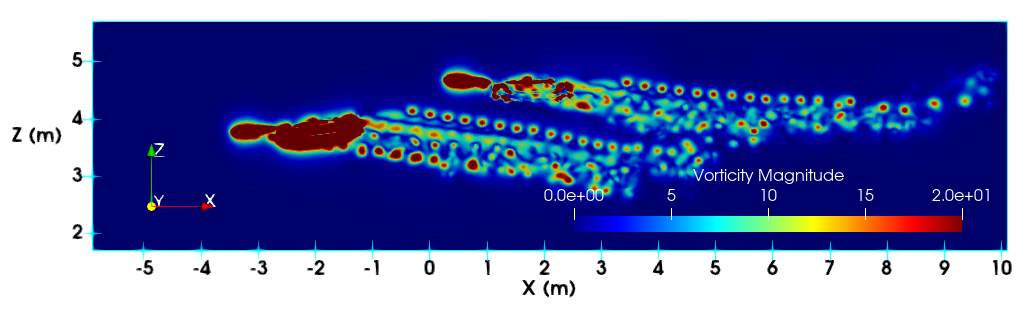
\includegraphics[width=7cm]{fig/figure_chap3/chap_3_5_4_2.png}}\quad
  \subfloat[下移0.7 m]{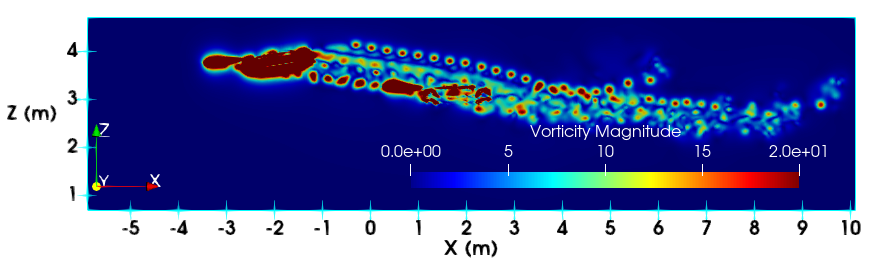
\includegraphics[width=7cm]{fig/figure_chap3/chap_3_5_4_3.png}}
  \caption{直升机协同吊挂系统不同垂向相对位置下的涡度场}
  \label{fig:chap3_5_4_1}
\end{figure}

图\ref{fig:chap3_5_4_2}给出了不同垂向相对位置下0.75 R处的截面力。当直升机1上移0.7 m时,从方位角100 \degree 到250 \degree,前旋翼的截面拉力相比其他两种情况更大、
波动更小。当直升机1下移0.7 m时,后旋翼的截面拉力比其他两种情况小。这是因为直升机1下移0.7 m时,直升机1完全沉浸在直升机4的尾流中。
\begin{figure}[!htb]
  \centering
  \subfloat[前旋翼]{\includegraphics[width=7cm]{fig/figure_chap3/chap_3_5_4_4.png}}\quad
  \subfloat[后旋翼]{\includegraphics[width=7cm]{fig/figure_chap3/chap_3_5_4_5.png}}
  \caption{不同垂向相对位置下0.75 R 处的截面力}
  \label{fig:chap3_5_4_2}
\end{figure}

图\ref{fig:chap3_5_4_3}(a)和图\ref{fig:chap3_5_4_4}(a)给出了不同垂向相对位置下直升机1前旋翼拉力和功率的变化。对于基础配置和直升机1下移0.7 m的情况,当垂向相对位置为0时,大约有20\%的拉力损失和15\%的功率增加。当直升机1和直升机4间的侧向相对位置正向或负向增加时,拉力增加,功率减小。对于直升机1上移0.7 m、上移1.4 m、下移1.4 m的情况,拉力、功率与无干扰时相差不大。

图\ref{fig:chap3_5_4_3}(b)和图\ref{fig:chap3_5_4_4}(b)给出了不同垂向相对位置下直升机1后旋翼拉力和功率的变化。可以看出,垂向相对位置变化对后旋翼拉力和功率的影响较小。

\begin{figure}[!htb]
  \centering
  \subfloat[前旋翼]{\includegraphics[width=7cm]{fig/figure_chap3/chap_3_5_4_6.png}}\quad
  \subfloat[后旋翼]{\includegraphics[width=7cm]{fig/figure_chap3/chap_3_5_4_7.png}}
  \caption{不同垂向相对位置下的旋翼拉力}
  \label{fig:chap3_5_4_3}
\end{figure}

\begin{figure}[!htb]
  \centering
  \subfloat[前旋翼]{\includegraphics[width=7cm]{fig/figure_chap3/chap_3_5_4_8.png}}\quad
  \subfloat[后旋翼]{\includegraphics[width=7cm]{fig/figure_chap3/chap_3_5_4_9.png}}
  \caption{不同垂向相对位置下的旋翼功率}
  \label{fig:chap3_5_4_4}
\end{figure}
\subsection{基于气动干扰分析的协同吊挂系统队形推荐}
基于上面的气动干扰分析,前进比为0.1时,直升机1和直升机4间的侧向相对位置处于-1.5到-0.75倍的旋翼直径、0.75到1.5倍的旋翼直径时,有利于减少气动干扰、降低拉力损失、减少功率消耗。当直升机1和直升机4间的纵向相对距离大于2.5倍的旋翼直径、后方直升机比前侧直升机高0.5倍的旋翼直径时,气动干扰大幅减少,有利于提高性能。此外,考虑到前进比0.1时对应气动干扰相对严重的情况,因此以上结论对悬停、前进比小于0.1时均适用。

因此,横纵向相对位置越大或后侧直升机比前侧直升机垂向位置高时,有利于减小直升机协同吊挂系统间的气动干扰。这意味着图\ref{fig:chap3_5_5_1}所示的梯形队形或后侧直升机相对较高的矩形队形更佳。
\begin{figure}[!htb]
  \centering
  \subfloat[梯形队形]{\includegraphics[width=6cm]{fig/figure_chap3/chap_3_5_5_1.png}}\quad
  \subfloat[矩形队形]{\includegraphics[width=8cm]{fig/figure_chap3/chap_3_5_5_2.png}}
  \caption{基于气动干扰分析的协同吊挂系统队形推荐}
  \label{fig:chap3_5_5_1}
\end{figure}

\section{本章小结}
本小节给出了直升机协同吊挂系统的配平方法,分析了整个系统的稳定性和操作性,并在配平基础了开展了系统的气动干扰分析,从气动干扰角度给出了直升机协同吊挂系统的推荐队形,对下文控制策略的设计、吊挂负载的合理分配等均奠定了基础。主要包括
\begin{enumerate}
  \item 在配平的基础了,基于涡方法分析了直升机协同吊挂系统的气动干扰情况,并指出本文研究的四直升机协同吊挂系统,前飞时的前后排列的直升机间气动干扰更为严重。为此,以前进比0.1(前飞速度10 m/s)为例,分析了不同侧向、纵向、垂向相对位置对气动干扰的影响。基于以上分析,指出从减小气动干扰的角度,梯形队形或后侧直升机相对较高的矩形队形更佳。
\end{enumerate}
% \chapter{以吊挂物为中心的直升机协同吊挂系统控制策略}
\section{引言}
\section{吊挂物控制策略设计}
\section{吊索层控制策略设计}
\subsection{吊索力计算}
\subsection{优化算法}
\section{直升机层控制策略设计}
\subsection{求解直升机目标飞行状态}
\subsection{基于改进自抗扰的直升机位置、姿态控制}
\section{仿真验证}
\subsection{吊挂物轨迹、绳索锥角设计}
\subsection{方案1仿真结果}
\subsection{方案2仿真结果}
\subsection{方案3仿真结果}
\section{本章小结}

% \chapter{基于功率消耗和鲁棒自适应博弈控制的负载分配策略}
在协同吊挂系统中,如果一个直升机在飞行过程中提前耗尽能量或失效,协同运输会直接崩溃。可见,在综合考虑各直升机相对位置、性能差异的前提下,合理分配吊挂负载给各个直升机,具有重要意义。为此,本文提出了基于功率消耗和鲁棒自适应博弈控制的负载分配策略。第\ref{section:chap_4_introduction}节首先以四个纵列式直升机协同吊挂系统为研究对象,基于以吊挂物为主导的分层控制策略,将负载分配问题分解为期望吊索拉力计算和抗干扰吊索拉力计算两部分。第\ref{section:power_distribution}节训练得到了直升机神经网络功率代理模型,提出了基于功率消耗的负载分配策略。第\ref{section:game_distribution}节考虑直升机性能差异、互动影响,提出了基于鲁棒自适应微分博弈控制的抗干扰负载分配策略。最后,仿真对比了基于功率消耗、绳索拉力的负载分配策略的优缺点;验证了各直升机性能存在差异时期望吊索拉力优化计算方法的可行性;针对不同值函数验证了博弈控制的可行性和鲁棒性;分析了基于整个分配策略的仿真结果。

\section{引言}\label{section:chap_4_introduction}
在直升机协同吊挂系统中,如果其中一架或几架直升机提前耗尽能量或发生故障,且吊挂物重量大于剩余直升机的负载能力时,整个协同吊挂系统将会失效,甚至发生吊索交叉、直升机相互碰撞等高危情况。所以,合理分配负载给各个直升机,使各个直升机在协同运输过程中功耗相等、航时航程一致,是必要的。

\begin{figure}[!htb]  
  \includegraphics[width=10cm]{fig/figure_chap4/Chap4_1_1.png}
  \caption{直升机协同吊挂系统分层控制技术}
  \label{fig:4_1_1}
\end{figure}

以吊挂物为主导的直升机协同吊挂系统分层控制技术(见图\ref{fig:4_1_1})主要包括以下三个方面:
\begin{enumerate}
  \item 吊挂物层:根据吊挂物期望轨迹和状态,计算需要吊索提供的期望合力、合力矩。同时考虑到外界环境干扰等,设计跟随控制控制律,计算需要吊索额外提供的抗干扰合力、合力矩。将两者相加,得到需要吊索提供的全部合力、合力矩。
  \item 吊索层:根据需要吊索提供的合力、合力矩,计算需要每根吊索提供的力。在某一特定飞行状态下,吊索拉力和方向直接影响各个直升机的功率消耗。
  \item 直升机层:根据需要每根吊索提供的力,计算各个直升机的期望位置。合理设计控制策略,跟随期望位置。
\end{enumerate}

假设路径已知,基于以吊挂物为主导的直升机协同吊挂系统分层控制技术,负载分配策略可以分为期望吊索力和抗干扰吊索力计算两部分。为此,考虑各个直升机性能、位置、状态、约束差异等,本文提出了基于功率消耗的稳态负载分配策略和基于鲁棒自适应博弈跟随控制的抗干扰分配策略。

\section{基于功率消耗的期望负载分配策略}\label{section:power_distribution}
以往多数文献大多采用基于吊索拉力相等的期望负载分配策略。但随着协同吊挂系统前飞速度的增加,吊索拉力相等并不能保证各个直升机功率消耗相等。可见,这种分配策略策略仅适用于悬停、小速度飞行或机动较小的情况。因此,提出基于功率消耗的期望负载分配策略,保证在整个飞行包线内各直升机功耗相等,是有重要意义的。
\subsection{功率代理模型}
直升机功率是在配平基础上计算得到的。各个直升机动力学模型中有30个状态量,配平本身就很困难。同时考虑到基于功率消耗的期望负载分配策略要用优化方法来解决,若每次迭代均在线配平计算功率消耗,复杂度高、计算时间长。为此,提出了基于BP神经网络的功率代理模型。
\subsubsection{功率计算与分析}
假设每个纵列式直升机的吊挂点均位于重心处。则对直升机$i$,在其体轴系$x_{ib}y_{ib}z_{ib}$下,吊索作用在直升机重心的吊索力和力矩为
\begin{equation}
  {{\mathbf{M}}_{cable,i}} = \left[ {\begin{array}{*{20}{c}}
    {^i{{\mathbf{R}}_e}{\;^e}{{\mathbf{R}}_L}{\;^L}{{\mathbf{f}}_{cable.i}}} \\ 
    {{{\mathbf{0}}_{3 \times 1}}} 
  \end{array}} \right]
\end{equation}
其中,${\;^i}{{\bf{R}}_e}$为轴系$x_{e}y_{e}z_{e}$到$x_{ib}y_{ib}z_{ib}$的转换矩阵。

\begin{figure}[!htb]
  \subfloat[悬停]{\includegraphics[width=7cm]{fig/figure_chap4/Chap4_2_1.png}}\quad
  \subfloat[前进比0.1]{\includegraphics[width=7cm]{fig/figure_chap4/Chap4_2_2.png}}
  \caption{功率消耗计算结果}
  \label{fig:4_2_1}
\end{figure}

在吊索力作用下,采用牛顿法配平各个直升机,进而根据配平得到的状态量和操纵量计算得到功率。以悬停和前进比0.1时的功率消耗为例,见图\ref{fig:4_2_1},可以看出,悬停时功率消耗主要与吊索拉力有关。这是以往文献中较多采用基于吊索拉力均等的负载分配策略的原因。

然而,前进比为0.1时,除吊索拉力外,角$\beta$也是重要影响因素。在“2-lead”协同吊挂系统中,前面两侧直升机(直升机3、4)角$\beta$处于-90\degree 到90\degree 之间,吊索拉力作用等同于对直升机施加向后的阻力,功率消耗大。后方直升机(直升机1、2)角$\beta$处于-180\degree 到-90\degree、90\degree 到180\degree 之间,吊索拉力作用等同于对直升机施加向前的拉力,功率消耗小。可见,有一定的前飞速度时,即使吊索拉力相同,前方直升机的功率依旧会大于后方直升机。这与参考文献\cite{enciu2017flight,song2013modeling}中的计算结果吻合。

此外,需要指出的是,直升机协同吊挂系统是典型的近距离编队飞行。直升机之间不仅存在复杂的动力学耦合关系,而且存在严重的气动干扰。根据之前的计算结果\cite{Duan2021Underreview}可知,前飞时的气动干扰最大,且由气动干扰引起的功率变化比较复杂、难以建模。此外,研究发现当纵列式直升机间的距离大于小2.5倍的旋翼直径时,针对本文研究的四纵列式直升机协同吊挂系统,气动干扰可以忽略不计。因此,本文没有将气动干扰引起的功率变化引入到代理模型中,而是将下文优化过程中直升机间的安全距离约束设置为了2.5倍的旋翼直径。
\subsubsection{基于神经网络的代理模型}
BP神经网络是典型多层前向网络,如图\ref{fig:4_2_2}所示,主要由信号正向传播和误差反向传播组成。正向传播指信号依次经过输入、隐层神经元,再由输出神经元输出的过程。反向传播是指,当输出值与目标值之间存在误差时,将误差反向传播,并由梯度下降算法更新网络权值、阈值的过程。当误差足够小时,网络反向传播停止,BP神经网络训练完成。
\begin{figure}[!htb]
  \includegraphics[width=8cm]{fig/figure_chap4/Chap4_2_3.png}
  \caption{BP神经网络}
  \label{fig:4_2_2}
\end{figure}

针对纵列式直升机神经网络功率代理模型,输入层有4个变量:前进比、角$\alpha$、角$\beta$、吊索拉力。根据问题复杂度,隐含层设计了40个神经元。神经网络输出为直升机的功率消耗。此外,隐含层的激活函数为双曲正切函数,输出层的激活函数为恒等映射函数。

用于训练功率代理模型的数据集前进比取值为0到0.11,角$\alpha$取值为0到$\frac{\pi}{2}$,角$\beta$取值为$-\pi$到$\pi$,吊索拉力取值为0到100 N(吊挂物重量)。经过上述过程,共得到4680个数据点,其中4000个数据点用来训练神经网络,剩余的680个数据点用来验证神经网络的有效性。从图\ref{fig:4_2_3}可以看出,真实值与神经网络输出值拟合很好。这表明训练得到的功率代理模型是有效的,可以在下文的优化工作中使用。
\begin{figure}[!htb]
  \includegraphics[width=7cm]{fig/figure_chap4/Chap4_2_4.png}
  \caption{基于BP神经网络的功率消耗拟合结果}
  \label{fig:4_2_3}
\end{figure}

\subsection{负载分配优化模型}
\subsubsection{设计变量}
针对4个纵列式直升机协同运输一个吊挂物的系统,选择4根吊索的力矢量作为设计变量,如下
\begin{equation}
  {\bf{u}} = \left[ {^L{f_{cable,1x}},{\;^L}{f_{cable,1y}},{\;^L}{f_{cable,1z}},\; \cdots ,{\;^L}{f_{cable,4x}},{\;^L}{f_{cable,4y}},{\;^L}{f_{cable,4z}}} \right]^T
\end{equation}
\subsubsection{约束}
首先,吊索力矢量需满足吊挂物的动力学方程,见式\ref{equation:chap_4_1}。将吊索作用力$\bf{M}_c$移到左侧,式\ref{equation:chap_4_1}也可以写作
\begin{equation}
  \left[ {\begin{array}{*{20}{c}}
    {{{\bf{I}}_{3 \times 3}}}&{{{\bf{I}}_{3 \times 3}}}&{{{\bf{I}}_{3 \times 3}}}&{{{\bf{I}}_{3 \times 3}}}\\
    {{{\left( {{{\bf{h}}_1}} \right)}^*}}&{{{\left( {{{\bf{h}}_2}} \right)}^*}}&{{{\left( {{{\bf{h}}_3}} \right)}^*}}&{{{\left( {{{\bf{h}}_4}} \right)}^*}}
    \end{array}} \right]{\bf{u}} = {{\bf{M}}_L}{\bf{\ddot x}} + {{\bf{C}}_L}{\bf{\dot x}} - {{\bf{g}}_L} - {{\bf{M}}_{aero}}
    \label{equation:chap_4_8}
\end{equation}
其中,${{{\left( {{{\bf{h}}_i}} \right)}^*}}$是向量${{{\bf{h}}_i}}$的斜对称矩阵。

为了避免直升机间相互碰撞、减少气动干扰,引入直升机间的安全距离约束如下
\begin{equation}
  \left\| {^e{{\bf{P}}_i} - {\;^e}{{\bf{P}}_j}} \right\| \ge {d_{\min }}\;\;\;\;\;\;\;\;\;i,j = 1,2,3,4
\end{equation}
其中,$d_{\min}$等于4.5 m(2.5倍的旋翼直径)。事实上,直升机间的距离越大,角$\alpha$越大,负载相同的吊挂物需要的吊索拉力越大。吊索拉力越大,直升机功率消耗也越大,这对优化目标是不利的。使用长吊索可以缓解这种不利情况,经过计算发现本文研究的四纵列式直升机协同吊挂系统中7.2 m的吊索长度是足够的。

为增加收敛速度,引入式\ref{equation:chap4_2_2_2_3}中的约束。同时,可以看出,通过设置垂向吊索力分量最大值为-0.05$m_Lg$,可以避免吊索松动;侧向吊索力分量约束可以减小吊索发生交叉的可能性。
\begin{equation}
  \begin{array}{l}
      \left[ \begin{array}{*{20}{c}}
          - 1 & - 1 & - 1 & - 1 & 0 & -1 & - 1 & 0 & - 1 & - 1 &- 1 & - 1\\\end{array} 
          \right]{m_L}g \le {{\bf{u}}} \le\\
      \left[ \begin{array}{*{20}{c}}
          1 & 0 & - 0.05 & 1 & 1 & -0.05& 1 & 1 & -0.05 & 1 & 0 & -0.05\\\end{array} 
          \right]{m_L}g \\       
  \end{array}
  \label{equation:chap4_2_2_2_3}
\end{equation}

此外,考虑到由路径规划引入的各直升机位置约束,增加角$\alpha$和$\beta$约束如下
\begin{equation}
  \left\{ \begin{array}{l}
    {\alpha _{i,\min }} \le {\alpha _i} \le {\alpha _{i,\max }}\\
    {\beta _{i,\min }} \le {\beta _i} \le {\beta _{i,\max }}
    \end{array} \right. \ \ i = 1,2,3,4
\end{equation}
其中,${\alpha _{i,\min }}$、${\alpha _{i,\max }} $分别为路径规划允许的的角$\alpha_i$的最大、最小值,${\beta _{i,\min }}$、${\beta _{i,\max }}$分别为路径规划允许的的角$\beta_i$的最大、最小值。

\subsubsection{目标函数}
为了基于功率消耗将负载平均分配给各直升机,同时考虑到直升机间的性能差异,设置目标函数为最小化功耗最大的直升机的等效功率,如下
\begin{equation}
  J = \min \left( {\max \left( {{k _i}{P_i}} \right)} \right)\;\;\;\;i = 1,2,3,4
  \label{equation:chap_4_12}
\end{equation}
其中,$P_i$代表直升机$i$的功率消耗,$k_i$是和等效功耗相关的缩放因子。比如,当功率消耗为500 W时,直升机1、2的航时分别为60、30分钟。那么$k_1$、$k_2$可分别设置为1、2,以避免直升机2过早消耗完能量。
\subsubsection{求解方法}
采用MATLAB/fmincon函数求解上述非线性数值优化问题。采用sqp(sequential quadratic programming)算法,鲁棒性强、计算效率高。设计变量、目标函数和约束的收敛边界分别设为1e-6、1e-6和1e-4。

\section{基于博弈跟随控制的负载分配策略}\label{section:game_distribution}
吊挂物作用于直升机的负载,除期望轨迹引起的期望吊索力外,还有一部分来自吊挂物跟随控制带来的负载。参与协同吊挂的直升机间可能存在性能配置差异等,各个直升机若采用同一目标函数,或者简单地将各个直升机的目标函数进行简单加权,不能充分考虑直升机间互动的影响,也不能充分发挥系统潜力。因此,本文提出了基于鲁棒博弈跟随控制的负载分配策略。此外,这部分负载多用来抵抗吊挂物运动过程中的干扰,与期望吊索力相比往往不在一个量级。同时考虑到功率计算复杂度和跟随控制的实时性需求,本文在确保跟随性的前提下,在微分博弈理论框架下采用最小化吊索力的方式求解这部分负载。

\subsection{微分博弈模型}
根据上一节内容,基于给定的吊挂物轨迹和状态,可以计算出期望吊索力,分别记为$\mathbf{x}_r$和$\mathbf{u}_r$。
在上述平衡点附近,进行小扰动假设得到雅克比矩阵,进而可以得到吊挂物的线性化模型,如下
\begin{equation}
  \begin{array}{l}
    \Delta \dot{\bf{x}} = f\left( {{{\bf{x}}_r} + \Delta {\bf{x}},\;{{\bf{u}}_r} + \Delta {\bf{u}}} \right) - f\left( {{{\bf{x}}_r},\;{{\bf{u}}_r}} \right)\\
    \;\;\;\; = \frac{{\partial f}}{{\partial {\bf{x}}}}\left| {_{\scriptstyle{\bf{x}} = {{\bf{x}}_r}\hfill\atop
    \scriptstyle{\bf{u}} = {{\bf{u}}_r}\hfill}} \right.\Delta {\bf{x}} + \frac{{\partial f}}{{\partial {\bf{u}}}}\left| {_{\scriptstyle{\bf{x}} = {{\bf{x}}_r}\hfill\atop
    \scriptstyle{\bf{u}} = {{\bf{u}}_r}\hfill}} \right.\Delta {\bf{u}}\\
    \;\;\;\; = {\bf{A}}\;\Delta {\bf{x}} + \;{\bf{B}}\;\Delta {\bf{u}}
    \end{array}
    \label{equation:chap_4_3_1}
\end{equation}
其中,$f = {{\bf{M}}_L}^{ - 1}\left( {{{\bf{g}}_L} + {{\bf{M}}_c} + {{\bf{M}}_{aero}} - {{\bf{C}}_L}{\bf{x}}} \right)$。为方便下文推导,定义$\Delta {\bf{x}} = {\bf{\tilde x}}$、$\Delta {\bf{u}} = {\bf{\tilde u}}$。

将干扰考虑在内,式\ref{equation:chap_4_3_1}可以重写为
\begin{equation}
  \dot{\tilde{\mathbf{x}}} = {\mathbf{A\tilde x}} + \sum\limits_{j = 1}^N {{{\mathbf{g}}_j}{{{\mathbf{\tilde u}}}_j}}  + {\mathbf{Dv}}
  \label{equation:chap_4_14}
\end{equation}
其中,$\tilde{\mathbf{u}}_j$为直升机$j$的控制量,$\mathbf{g}_j$是矩阵$\mathbf{B}$的第$3j-2$到第$3j$列,$\mathbf{v}$代表由外界环境和系统未建模因素引起的干扰,$\mathbf{D}$定义如下
\begin{equation}
  {\mathbf{D}} = \left[ {\begin{array}{*{20}{c}}
    {{{\mathbf{0}}_{3 \times 3}}}&{{{\mathbf{0}}_{3 \times 3}}} \\ 
    {{{\mathbf{0}}_{3 \times 3}}}&{{{\mathbf{0}}_{3 \times 3}}} \\ 
    {m_L^{ - 1}{{\mathbf{I}}_{3 \times 3}}}&{{{\mathbf{0}}_{3 \times 3}}} \\ 
    {{{\mathbf{0}}_{3 \times 3}}}&{{\mathbf{J}}_L^{ - 1}} 
  \end{array}} \right]
\end{equation}

为了设计鲁棒控制器,可以将各个直升机的性能函数定义为
\begin{equation}
  {J_i}\left( {{{{\mathbf{\tilde x}}}_0},{{{\mathbf{\tilde u}}}_i},{{{\mathbf{\tilde u}}}_{\hat i}},{\mathbf{v}}} \right) = \int_0^\infty  {\left( {{{{\mathbf{\tilde x}}}^T}{{\mathbf{Q}}_i}{\mathbf{\tilde x}} + \sum\limits_{j = 1}^N {{{{\mathbf{\tilde u}}}_j}^T{{\mathbf{R}}_{ij}}{{{\mathbf{\tilde u}}}_j} - {\gamma ^2}{{\mathbf{v}}^T}{{\mathbf{T}}_i}{\mathbf{v}}} } \right)} \;dt\;\;\;\;i \in \mathbb{N}
  \label{equation:chap_4_16}
\end{equation}
其中,${{\bf{\tilde x}}_0}$为${\bf{\tilde x}}$的初始值,${{\bf{\tilde u}}_{\hat i}}$为除直升机$i$外其余直升机的控制量。${{\mathbf{Q}}_i} \in {\mathbb{R}^{6 \times 6}}$、${{\mathbf{R}}_{ij}} \in {\mathbb{R}^{3 \times 3}}$、${{\mathbf{T}}_i} \in {\mathbb{R}^{3 \times 3}}$均为正定矩阵,$\gamma $是给定正常数。式\ref{equation:chap_4_16}第一项${{\mathbf{\tilde x}}^T}{{\mathbf{Q}}_i}{\mathbf{\tilde x}}$为状态偏差量惩罚项,${{\bf{\tilde u}}_j}^T{{\bf{R}}_{ij}}{{\bf{\tilde u}}_j}$为直升机$j$相对于直升机$i$的控制量惩罚项,$- {\gamma ^2}{{\mathbf{v}}^T}{{\mathbf{T}}_i}{\mathbf{v}}$是从直升机$i$角度引入的干扰量惩罚项。

直升机$i$的目标为与其他直升机协同吊挂负载的同时,寻找控制策略优化式\ref{equation:chap_4_16}。假设系统信息对各个直升机是完全已知的,${{\bf{Q}}_i}$、${{\bf{R}}_{ij}}$、${{\bf{T}}_i}$为不随时间变化的权重矩阵。

经过以上分析,并将干扰看作参与博弈的独立个体,上述控制问题可以转换为微分博弈的形式,如下
\begin{equation}
  {V_i}\left( {{{{\mathbf{\tilde x}}}_0}} \right) = \mathop {\min }\limits_{{{{\mathbf{\tilde u}}}_i}} \mathop {\max }\limits_{\mathbf{v}} {J_i}\left( {{{{\mathbf{\tilde x}}}_0},{{{\mathbf{\tilde u}}}_i},{{{\mathbf{\tilde u}}}_{\hat i}},{\mathbf{v}}} \right)\;\;\;\;i \in \mathbb{N}
\end{equation}

接着,上述博弈问题可以转化为最优值函数的形式,如下
\begin{equation}
  \begin{gathered}
    {V_i}^*\left( {{{{\mathbf{\tilde x}}}_0}} \right) = \mathop {\min }\limits_{{{{\mathbf{\tilde u}}}_i}} \mathop {\max }\limits_{\mathbf{v}} {J_i}\left( {{{{\mathbf{\tilde x}}}_0},{{{\mathbf{\tilde u}}}_i},{{{\mathbf{\tilde u}}}^*}_{\hat i},{\mathbf{v}}} \right) \hfill \\
    \;\;\;\;\;\;\;\;\;\; = \mathop {\max }\limits_{\mathbf{v}} \mathop {\min }\limits_{{{{\mathbf{\tilde u}}}_i}} {J_i}\left( {{{{\mathbf{\tilde x}}}_0},{{{\mathbf{\tilde u}}}_i},{{{\mathbf{\tilde u}}}^*}_{\hat i},{\mathbf{v}}} \right),\;\;\;\;i \in \mathbb{N} \hfill \\ 
  \end{gathered} 
\end{equation}
其中,${V_i}^*$是直升机$i$的最优值函数,$\left( {{\bf{\tilde u}}_i^*,{{{\bf{\tilde u}}}^*}_{\hat i}} \right)$是纳什均衡控制策略解。
\subsection{鲁棒纳什均衡解}
\textbf{定义1鲁棒纳什均衡解}\cite{de2017finite}:如果${{\bf{\tilde u}}_i}^*$和${{\bf{\tilde u}}_{\hat i}}^*$满足以下$N$个不等式,则称其为鲁棒纳什均衡解。
\begin{equation}
  {J_i}\left( {{\mathbf{\tilde x}},{{{\mathbf{\tilde u}}}_i}^*,{{{\mathbf{\tilde u}}}_{\hat i}}^*,{\mathbf{v}}} \right) \leqslant {J_i}\left( {{\mathbf{\tilde x}},{{{\mathbf{\tilde u}}}_i}^*,{{{\mathbf{\tilde u}}}_{\hat i}}^*,{{\mathbf{v}}^*}} \right) \leqslant {J_i}\left( {{\mathbf{\tilde x}},{{{\mathbf{\tilde u}}}_i},{{{\mathbf{\tilde u}}}_{\hat i}}^*,{{\mathbf{v}}^*}} \right)\;\;\;\;i \in \mathbb{N}
\end{equation}
其中,${{\bf{v}}^*}$对应最坏情况下的干扰量。

给定${{\bf{\tilde u}}_i}$和${\bf{v}}$,直升机$i$的值函数可以表示为
\begin{equation}
  {V_i}\left( {{\mathbf{\tilde x}}\left( t \right)} \right) = \int_t^\infty  {\left( {{{{\mathbf{\tilde x}}}^T}{{\mathbf{Q}}_i}{\mathbf{\tilde x}} + \sum\limits_{j = 1}^N {{{{\mathbf{\tilde u}}}_j}^T{{\mathbf{R}}_{ij}}{{{\mathbf{\tilde u}}}_j} - {\gamma ^2}{{\mathbf{v}}^T}{{\mathbf{T}}_i}{\mathbf{v}}} } \right)} \;d\tau \;\;\;i \in \mathbb{N}
  \label{equation:chap_4_1_20}
\end{equation}

对式\ref{equation:chap_4_1_20}两边求导,可得哈密顿方程如下
\begin{equation}
  \begin{gathered}
    {H_i}\left( {{\mathbf{\tilde x}},\nabla {{\mathbf{V}}_i},{{{\mathbf{\tilde u}}}_i},{{{\mathbf{\tilde u}}}_{\hat i}},{\mathbf{v}}} \right) = \left( {{{{\mathbf{\tilde x}}}^T}{{\mathbf{Q}}_i}{\mathbf{\tilde x}} + \sum\limits_{j = 1}^N {{{{\mathbf{\tilde u}}}_j}^T{{\mathbf{R}}_{ij}}{{{\mathbf{\tilde u}}}_j} - {\gamma ^2}{{\mathbf{v}}^T}{{\mathbf{T}}_i}{\mathbf{v}}} } \right) \hfill \\
    \;\;\;\;\;\;\;\;\;\;\;\;\;\;\;\;\;\;\;\;\;\;\;\;\;\;\;\;\; + {\left( {\nabla {{\mathbf{V}}_i}} \right)^T}\left( {{\mathbf{A\tilde x}} + \sum\limits_{j = 1}^N {{{\mathbf{g}}_j}{{{\mathbf{\tilde u}}}_j} + {\mathbf{Dv}}} } \right)\;\;\;i \in \mathbb{N} \hfill \\ 
  \end{gathered} 
  \label{equation:chap_4_21}
\end{equation}
其中,$\nabla {{\bf{V}}_i} = \frac{{\partial {{\bf{V}}_i}}}{{\partial {\bf{\tilde x}}}}$。然后可以得到鲁棒纳什均衡解反馈控制策略,如下
\begin{equation}
  \left\{ \begin{gathered}
    \frac{{\partial {H_i}}}{{\partial {{{\mathbf{\tilde u}}}_i}}} = 0 \Rightarrow {{{\mathbf{\tilde u}}}_i}^* =  - \frac{1}{2}{\mathbf{R}}_{ii}^{ - 1}{\mathbf{g}}_i^T\;\nabla {\mathbf{V}}_i^*\;\;\;\;\;\;\;i \in \mathbb{N} \hfill \\
    \frac{{\partial {H_i}}}{{\partial {\mathbf{v}}}} = 0 \Rightarrow {{\mathbf{v}}^*} = \frac{1}{{2{\gamma ^2}}}{\mathbf{T}}_i^{ - 1}{{\mathbf{D}}^T}\;\nabla {\mathbf{V}}_i^*\;\;\;\;\;\;\;i \in \mathbb{N} \hfill \\ 
  \end{gathered}  \right.
  \label{equation:chap_4_22}
\end{equation}

将式\ref{equation:chap_4_22}代入式\ref{equation:chap_4_21},可以得到$N$个耦合的哈密顿方程组。在$N$个耦合的哈密顿方程组中,有$N$个未知量$\nabla {\bf{V}}_i^*$,$i \in \mathbb{N}$。一旦确定$\nabla {\bf{V}}_i^*$的值,就可以根据式\ref{equation:chap_4_22}计算得到反馈控制策略。然而$N$个耦合的哈密顿方程组是高度耦合的,很难求解。因此,本文引入自适应学习策略来在线拟合$\nabla {\bf{V}}_i^*$。

\subsection{自适应学习策略}
根据神经网络自适应学习策略,最优值函数可以写成
\begin{equation}
  {V_i}\left( {{\mathbf{\tilde x}}} \right) = {\mathbf{W}}_i^T{{\mathbf{\delta }}_i}\left( {{\mathbf{\tilde x}}} \right) + {\varepsilon _i}\left( {{\mathbf{\tilde x}}} \right)
  \label{equation:chap_4_23}
\end{equation}
其中,${{\mathbf{W}}_i} \in {\mathbb{R}^K}$为期望权值矢量,${{\mathbf{\delta }}_i} \in {\mathbb{R}^K}$是激活函数矢量,${\varepsilon _i} \in \mathbb{R}$是重构误差,$K$代表神经元的个数。对式\ref{equation:chap_4_23}两边相对向量${\mathbf{\tilde x}}$求导,可得
\begin{equation}
  \nabla {{\mathbf{V}}_i} = \nabla {\mathbf{\delta }}_i^T{{\mathbf{W}}_i} + \nabla {{\mathbf{\varepsilon }}_i}\left( {{\mathbf{\tilde x}}} \right)
  \label{equation:chap_4_24}
\end{equation}
其中,$\nabla {{\mathbf{\delta }}_i} \in {\mathbb{R}^{K \times 12}}$,$\nabla {{\mathbf{\varepsilon }}_i} \in {\mathbb{R}^{12}}$。

考虑到${{\mathbf{W}}_i}$是未知的,式\ref{equation:chap_4_23}和\ref{equation:chap_4_24}可以转化为
\begin{equation}
  {\hat V_i}\left( \mathbf{\tilde x} \right) = {\mathbf{\hat W}}_i^T{{\mathbf{\delta }}_i}\left( \mathbf{\tilde x} \right)
  \label{equation:chap_4_25}
\end{equation}
\begin{equation}
  \nabla {{\mathbf{\hat V}}_i} = \nabla {\mathbf{\delta }}_i^T{{\mathbf{\hat W}}_i}
  \label{equation:chap_4_26}
\end{equation}
其中,${{\mathbf{\hat W}}_i}$为权值矢量估计值。将式\ref{equation:chap_4_26}代入式\ref{equation:chap_4_22},可得
\begin{equation}
  \left\{ \begin{gathered}
    {\hat{{\mathbf{\tilde u}}}_i}^*  =  - \frac{1}{2}{\mathbf{R}}_{ii}^{ - 1}{\mathbf{g}}_i^T\;\nabla {\mathbf{\delta }}_i^T{{{\mathbf{\hat W}}}_i}\;\;\;\;\;\;i \in \mathbb{N} \hfill \\
    {\hat{\mathbf{v}}^*} = \frac{1}{{2{\gamma ^2}}}{\mathbf{T}}_i^{ - 1}{{\mathbf{D}}^T}\;\nabla {\mathbf{\delta }}_i^T{{{\mathbf{\hat W}}}_i}\;\;\;\;\;\;i \in \mathbb{N} \hfill \\ 
  \end{gathered}  \right.
  \label{equation:chap_4_27}
\end{equation}

接着,将式\ref{equation:chap_4_27}代入式\ref{equation:chap_4_21},耦合哈密顿方程组可以重写为
\begin{equation}
  \begin{gathered}
    {H_i}\left( {{\mathbf{\tilde x}},{{{\mathbf{\hat W}}}_1}, \cdots ,{{{\mathbf{\hat W}}}_N}} \right) = {{{\mathbf{\tilde x}}}^T}{{\mathbf{Q}}_i}{\mathbf{\tilde x}} + \frac{1}{4}\sum\limits_{j = 1}^N {{\mathbf{\hat W}}_j^T\nabla {{\mathbf{\delta }}_j}{{\mathbf{g}}_j}{\mathbf{R}}_{jj}^{ - 1}{{\mathbf{R}}_{ij}}{\mathbf{R}}_{jj}^{ - 1}{\mathbf{g}}_j^T\;\nabla {\mathbf{\delta }}_j^T{{{\mathbf{\hat W}}}_j}}  \hfill \\
    \;\;\;\;\;\;\;\;\;\;\;\;\;\;\;\;\;\;\;\;\;\;\;\;\;\;\; - \frac{1}{{4{\gamma ^2}}}{\mathbf{\hat W}}_i^T\nabla {{\mathbf{\delta }}_i}{\mathbf{DT}}_i^{ - 1}{{\mathbf{D}}^T}\;\nabla {\mathbf{\delta }}_i^T{{{\mathbf{\hat W}}}_i}\; \hfill \\
    \;\;\;\;\;\;\;\;\;\;\;\;\;\;\;\;\;\;\;\;\;\;\;\;\;\;\; + {\mathbf{\hat W}}_i^T\nabla {{\mathbf{\delta }}_i}{\mathbf{A\tilde x}} - \frac{1}{2}{\mathbf{\hat W}}_i^T\nabla {{\mathbf{\delta }}_i}\sum\limits_{j = 1}^N {{{\mathbf{g}}_j}{\mathbf{R}}_{jj}^{ - 1}{\mathbf{g}}_j^T\;\nabla {\mathbf{\delta }}_j^T{{{\mathbf{\hat W}}}_j}}  \hfill \\
    \;\;\;\;\;\;\;\;\;\;\;\;\;\;\;\;\;\;\;\;\;\;\;\;\;\;\; + \frac{1}{{2{\gamma ^2}}}{\mathbf{\hat W}}_i^T\nabla {{\mathbf{\delta }}_i}{\mathbf{DT}}_i^{ - 1}{{\mathbf{D}}^T}\;\nabla {\mathbf{\delta }}_i^T{{{\mathbf{\hat W}}}_i}\;\; \hfill \\
    \;\;\;\;\;\;\;\;\;\;\;\;\;\;\;\;\;\;\;\;\;\;\;\;\; \triangleq {e_i}\;\;\;i \in \mathbb{N} \hfill \\ 
  \end{gathered} 
\end{equation}

设置性能指标为:
\begin{equation}
  {E_i} = \frac{1}{2}e_i^2
\end{equation}

根据梯度下降原则,可以得到如下的权值矢量更新策略
\begin{equation}
  {\dot{\bf{\hat W}}_i} =  - {\eta _i}\frac{{\partial {E_i}}}{{\partial {{{\bf{\hat W}}}_i}}} =  - {\eta _i}{e_i}{{\bf{\theta }}_i}
  \label{equation:chap_4_30}
\end{equation}
其中,${\eta _i}$为神经网络的学习速度参数,此外
\begin{equation}
  {{\bf{\theta }}_i} = \nabla {{\bf{\delta }}_i}\left( {{\bf{A\tilde x}} - \frac{1}{2}\sum\limits_{j = 1}^N {{{\bf{g}}_j}{\bf{R}}_{jj}^{ - 1}{\bf{g}}_j^T\;\nabla {\bf{\delta }}_j^T{{{\bf{\hat W}}}_j} + \frac{1}{{2{\gamma ^2}}}{\bf{DT}}_i^{ - 1}{{\bf{D}}^T}\;\nabla {\bf{\delta }}_i^T{{{\bf{\hat W}}}_i}} } \right)
\end{equation}

在此基础上,先根据式\ref{equation:chap_4_30}更新${{\mathbf{\hat W}}_i}$,然后鲁棒纳什均衡解可以通过式\ref{equation:chap_4_27}求解得到。
\subsection{稳定性分析}
\textbf{定理1:}考虑如式\ref{equation:chap_4_14}所示的线性系统,采用式\ref{equation:chap_4_27}的控制策略和式\ref{equation:chap_4_30}的更新策略,则闭环系统是稳定的。

\textbf{证明:}定义李雅普诺夫函数如下
\begin{equation}
  L = \sum\limits_{i = 1}^N {{L_i}\left( t \right)}  = \sum\limits_{i = 1}^N {\frac{1}{{2{\eta _i}}}{{{\bf{\tilde W}}}_i}^T{{{\bf{\tilde W}}}_i}} 
  \label{equation:chap_4_32}
\end{equation}
其中,${{\mathbf{\tilde W}}_i} = {{\mathbf{W}}_i} - {{\mathbf{\hat W}}_i}$。对式\ref{equation:chap_4_32}两边相对时间求导可得
\begin{equation}
  {\dot L_i}\left( t \right) = \frac{1}{{{\eta _i}}}{{\bf{\tilde W}}_i}^T{\dot{\bf{\tilde W}}_i}
  \label{equation:chap_4_33}
\end{equation}
其中,
\begin{equation}
  {\dot{\bf{\tilde W}}_i} =  - {\dot{\bf{\hat W}}_i} = {\eta _i}{e_i}{{\bf{\theta }}_i}
  \label{equation:chap_4_34}
\end{equation}

将式\ref{equation:chap_4_34}代入式\ref{equation:chap_4_33},${\dot L_i}\left( t \right)$可以重写为
\begin{equation}
  \begin{array}{l}
    {{\dot L}_i}\left( t \right) = {{{\bf{\tilde W}}}_i}^T{{\bf{\theta }}_i}{e_i}\\
     =  - \left( {{\bf{\tilde W}}_i^T{\bf{\theta }}_i^*} \right)\left( {{\bf{\tilde W}}_i^T{\bf{\theta }}_i^*} \right) - \left( {{\bf{\tilde W}}_i^T{\bf{\theta }}_i^*} \right)\left( {\sum\limits_{j = 1}^N {{\bf{\tilde W}}_i^T{{\bf{D}}_{ij}}{{{\bf{\tilde W}}}_j}} } \right) + \left( {{\bf{\tilde W}}_i^T{\bf{\theta }}_i^*} \right)\left( {\frac{1}{{2{\gamma ^2}}}{\bf{\tilde W}}_i^T{{\bf{F}}_{ij}}{{{\bf{\tilde W}}}_i}} \right)\\
    \;\; - \left( {\frac{1}{2}\sum\limits_{j = 1}^N {{\bf{\tilde W}}_i^T{{\bf{D}}_{ij}}{{{\bf{\tilde W}}}_j} - \frac{1}{{2{\gamma ^2}}}{\bf{\tilde W}}_i^T{{\bf{F}}_{ij}}{{{\bf{\tilde W}}}_i}} } \right)\left( {\frac{1}{2}\sum\limits_{j = 1}^N {{\bf{\tilde W}}_i^T{{\bf{D}}_{ij}}{{{\bf{\tilde W}}}_j} - \frac{1}{{2{\gamma ^2}}}{\bf{\tilde W}}_i^T{{\bf{F}}_{ij}}{{{\bf{\tilde W}}}_i}} } \right)\\
    \;\; + \left( {{\bf{\tilde W}}_i^T{{\bf{\theta }}_i}} \right)\left( {\frac{1}{4}\sum\limits_{j = 1}^N {{\bf{\tilde W}}_j^T{{\bf{E}}_{ij}}{{{\bf{\tilde W}}}_j}} } \right) + \left( {{\bf{\tilde W}}_i^T{{\bf{\theta }}_i}} \right)\left( {\frac{1}{2}\sum\limits_{j = 1}^N {{\bf{W}}_i^T{{\bf{D}}_{ij}}{{{\bf{\tilde W}}}_j}} } \right) - \frac{1}{{2{\gamma ^2}}}\left( {{\bf{\tilde W}}_i^T{{\bf{\theta }}_i}} \right){\bf{W}}_i^T{{\bf{F}}_{ij}}{{{\bf{\tilde W}}}_i}\\
    \;\; - \left( {{\bf{\tilde W}}_i^T{{\bf{\theta }}_i}} \right)\left( {\frac{1}{2}\sum\limits_{j = 1}^N {{\bf{W}}_j^T{{\bf{E}}_{ij}}{{{\bf{\tilde W}}}_j}} } \right)\; + \left( {{\bf{\tilde W}}_i^T{{\bf{\theta }}_i}} \right){e_{{H_i}}}
    \end{array}
    \label{equation:chap_4_35}
\end{equation}
其中,${e_{{H_i}}}$代表期望权值矢量下哈密顿函数的值,此外
\begin{equation}
  \left\{ \begin{array}{l}
    {{\bf{D}}_{ij}} = \nabla {{\bf{\delta }}_j}{{\bf{g}}_j}{\bf{R}}_{jj}^{ - 1}{\bf{g}}_j^T\;\nabla {\bf{\delta }}_j^T\\
    {{\bf{E}}_{ij}} = \nabla {{\bf{\delta }}_j}{{\bf{g}}_j}{\bf{R}}_{jj}^{ - 1}{{\bf{R}}_{ij}}{\bf{R}}_{jj}^{ - 1}{\bf{g}}_j^T\;\nabla {\bf{\delta }}_j^T\\
    {{\bf{F}}_{ij}} = \frac{1}{{2{\gamma ^2}}}\nabla {{\bf{\delta }}_i}{\bf{DT}}_i^{ - 1}{{\bf{D}}^T}\;\nabla {\bf{\delta }}_i^T
    \end{array} \right.
\end{equation}

假设$\left\| {{{\mathbf{D}}_{ij}}} \right\| \leqslant {\lambda _{DMij}}$,$\left\| {{{\mathbf{E}}_{ij}}} \right\| \leqslant {\lambda _{EMij}}$,$\left\| {{e_{{H_i}}}} \right\| \leqslant {b_{{e_{{H_i}}}}}$,$\left\| {{\mathbf{W}}_i^T{{\mathbf{D}}_{ij}}} \right\| \leqslant {b_{Dij}}$,$\left\| {{\mathbf{W}}_i^T{{\mathbf{F}}_{ij}}} \right\| \leqslant {b_{Fij}}$,$\left\| {{\mathbf{W}}_j^T{{\mathbf{F}}_{ij}}} \right\| \leqslant {b_{Eij}}$,${\theta _{im}} \leqslant \left\| {\theta _i^*} \right\| \leqslant {\theta _{iM}}$,${b_{im}} \leqslant \left\| {{\theta _i}} \right\| \leqslant {b_{iM}}$。其中,${\lambda _{DMij}}$,${\lambda _{EMij}}$,${b_{{e_{{H_i}}}}}$,${b_{Dij}}$,${b_{Fij}}$,${b_{Eij}}$,${\theta _{im}}$,${\theta _{iM}}$,${b_{im}}$,${b_{iM}}$均为正常数。随后,式\ref{equation:chap_4_35}中的第一项可以转化为
\begin{equation}
  - \left( {{\bf{\tilde W}}_i^T{\bf{\theta }}_i^*} \right)\left( {{\bf{\tilde W}}_i^T{\bf{\theta }}_i^*} \right) \le  - \theta _{im}^2{\left\| {{{{\bf{\tilde W}}}_i}} \right\|^2}
\end{equation}

式\ref{equation:chap_4_35}中的第四项满足如下不等式
\begin{equation}
  \sum\limits_{i = 1}^N {\left( { - \left( {\frac{1}{2}\sum\limits_{j = 1}^N {{\bf{\tilde W}}_i^T{{\bf{D}}_{ij}}{{{\bf{\tilde W}}}_j} - \frac{1}{{2{\gamma ^2}}}{\bf{\tilde W}}_i^T{{\bf{F}}_{ij}}{{{\bf{\tilde W}}}_i}} } \right)\left( {\frac{1}{2}\sum\limits_{j = 1}^N {{\bf{\tilde W}}_i^T{{\bf{D}}_{ij}}{{{\bf{\tilde W}}}_j} - \frac{1}{{2{\gamma ^2}}}{\bf{\tilde W}}_i^T{{\bf{F}}_{ij}}{{{\bf{\tilde W}}}_i}} } \right)} \right)}  \le  - {{\bf{Z}}^T}{{\bf{M}}_1}{\bf{Z}}
\end{equation}
其中,$Z \triangleq {\left[ {{{\left\| {{{{\mathbf{\tilde W}}}_1}} \right\|}^2}, \cdots ,{{\left\| {{{{\mathbf{\tilde W}}}_N}} \right\|}^2}} \right]^T} \in {\mathbb{R}^N}$,${{\mathbf{M}}_1}$是正定矩阵。

式\ref{equation:chap_4_35}中的其他项都可以写成两项相乘的形式。以第三项为例,满足以下条件
\begin{equation}
   - \left( {{\bf{\tilde W}}_i^T{\bf{\theta }}_i^*} \right)\left( {\sum\limits_{j = 1}^N {{\bf{\tilde W}}_i^T{{\bf{D}}_{ij}}{{{\bf{\tilde W}}}_j}} } \right) =  - \left( {{\bf{\tilde W}}_i^T{\bf{\theta }}_i^*} \right)\left( {{\bf{\tilde W}}_i^T{{\bf{D}}_{i1}}{{{\bf{\tilde W}}}_1} +  \cdots  + {\bf{\tilde W}}_i^T{{\bf{D}}_{iN}}{{{\bf{\tilde W}}}_N}} \right)
\end{equation}
\begin{equation}
  \begin{array}{l}
    - \left( {{\bf{\tilde W}}_i^T{\bf{\theta }}_i^*} \right)\left( {{\bf{\tilde W}}_i^T{{\bf{D}}_{ik1}}{{{\bf{\tilde W}}}_{k1}}} \right) =  - \frac{1}{2}\left( {{{\left( {{\psi _{i2k1}}\left( {{\bf{\tilde W}}_i^T{\bf{\theta }}_i^*} \right) + \frac{1}{{{\psi _{i2k1}}}}\left( {{\bf{\tilde W}}_i^T{{\bf{D}}_{ik1}}{{{\bf{\tilde W}}}_{k1}}} \right)} \right)}^2}} \right.\\
   \;\;\;\;\;\;\;\;\;\;\;\;\;\;\;\;\;\;\;\;\;\;\;\;\;\;\;\;\;\;\;\;\;\left. { - \psi _{_{i2k1}}^2{{\left( {{\bf{\tilde W}}_i^T{\bf{\theta }}_i^*} \right)}^2} - \frac{1}{{\psi _{_{i2k1}}^2}}{{\left( {{\bf{\tilde W}}_i^T{{\bf{D}}_{ik1}}{{{\bf{\tilde W}}}_{k1}}} \right)}^2}} \right)\\
   \;\;\;\;\;\;\;\;\;\;\;\;\;\;\;\;\;\;\;\;\;\;\;\;\;\;\;\;\;\;\; \le \frac{{\psi _{_{i2k1}}^2\theta _{iM}^2}}{2}{\left\| {{{{\bf{\tilde W}}}_i}} \right\|^2} + \frac{{\lambda _{DMik1}^2}}{{2\psi _{_{i2k1}}^2}}{\left\| {{{{\bf{\tilde W}}}_i}} \right\|^2}{\left\| {{{{\bf{\tilde W}}}_{k1}}} \right\|^2}
   \end{array}
\end{equation}
其中,${\psi _{i2k1}}$为不等于0的可调参数。将各项相加,可得
\begin{equation}
  \dot L\left( t \right) = \sum\limits_{i = 1}^N {{{\dot L}_i}\left( t \right)}  \le  - {{\bf{Z}}^T}{\bf{MZ}} + {\bf{TZ}} + K
\end{equation}
其中,${\lambda _m} \leqslant \left\| {\mathbf{M}} \right\| \leqslant {\lambda _M}$,$\left\| {\mathbf{T}} \right\| \leqslant {T_M}$,$\left\| K \right\| \leqslant {K_M}$。${\lambda _m}$、${\lambda _M}$、${T_M}$、${K_M}$均为正常数。
\begin{equation}
  \left\| Z \right\| > \frac{{{T_M} + \sqrt {T_M^2 + 4{\lambda _M}{K_M}} }}{{2{\lambda _M}}}
  \label{equation:chap_4_42}
\end{equation}

因此,只要式\ref{equation:chap_4_42}中的不等式得以满足,$\dot L\left( t \right) < 0$。此时,系统在李雅普诺夫意义下是渐近稳定的。此外,可以看出此时$\left\| Z \right\|$是一致最终有界的,进一步可知$\left\| {{{{\mathbf{\tilde W}}}_i}} \right\|$也是一致最终有界的。
\section{仿真结果与分析}
本节以四个直升机协同吊挂负载前飞80 m、侧飞10 m、下降10 m为任务需求,开展仿真分析。

基于任务需求设计了吊挂物轨迹;对比分析了基于功率消耗、绳索拉力的负载分配策略;开展了直升机存在差异时基于等效功率分配策略的仿真分析;针对不同值函数验证了博弈控制的可行性和鲁棒性;在此基础上,开展了整个负载分配策略仿真,验证了其有效性。

\begin{figure}[!htb]  
  \subfloat[位置]{\includegraphics[width=7cm]{chap4_5_1_1.png}}\quad
    \subfloat[速度]{\includegraphics[width=7cm]{chap4_5_1_2.png}}\\
    \subfloat[加速度]{\includegraphics[width=7cm]{chap4_5_1_3.png}}\quad
    \caption{设计的吊挂物轨迹}
    \label{fig:chap4_5_1_1}
  \end{figure}
\subsection{吊挂物轨迹}
由吊挂物气动特性可知,吊挂物姿态角为0时,阻力最小。因此,设计吊挂物期望姿态角始终为0。以初始点速度、加速度均为0为约束,基于三阶多项式生成了吊挂物的轨迹,见图\ref{fig:chap4_5_1_1}。

可见,10 s时,有最大前飞速度7.5 m/s, 对应前进比0.07。此时,前后直升机的状态有较大差异,可用来对比分析基于功率消耗、绳索拉力的负载分配策略的优缺点。4 s时,有最大前向加速度1.2 $\rm{m/s^2}$;16 s时,有最小前向加速度-1.2 $\rm{m/s^2}$。
  
\subsection{基于功率消耗的负载分配仿真结果}
\subsubsection{基于功率消耗与吊索拉力相等的分配策略仿真结果对比}
\begin{figure}[!htb]
  \subfloat[绳索拉力]{\includegraphics[width=7cm]{chap4_5_2_1.png}}\quad
  \subfloat[功率消耗]{\includegraphics[width=7cm]{chap4_5_2_2.png}}\\
  \subfloat[$\alpha$]{\includegraphics[width=7cm]{chap4_5_2_3.png}}\quad
  \subfloat[$\beta$]{\includegraphics[width=7cm]{chap4_5_2_4.png}}\\
  \subfloat[直升机间的距离]{\includegraphics[width=7cm]{chap4_5_2_5.png}}\quad
  \subfloat[轨迹]{\includegraphics[width=7cm]{chap4_5_2_6.png}}
  \caption{基于功率消耗分配策略的协同吊挂系统计算结果}
  \label{fig:chap4_5_2_1}
\end{figure}

\begin{figure}[!htb]
  \subfloat[绳索拉力]{\includegraphics[width=7cm]{chap4_5_2_7.png}}\quad
  \subfloat[功率消耗]{\includegraphics[width=7cm]{chap4_5_2_8.png}}\\
  \subfloat[$\alpha$]{\includegraphics[width=7cm]{chap4_5_2_9.png}}\quad
  \subfloat[$\beta$]{\includegraphics[width=7cm]{chap4_5_2_10.png}}\\
  \subfloat[直升机间的距离]{\includegraphics[width=7cm]{chap4_5_2_11.png}}\quad
  \subfloat[轨迹]{\includegraphics[width=7cm]{chap4_5_2_12.png}}
  \caption{基于绳索拉力分配策略的协同吊挂系统计算结果}
  \label{fig:chap4_5_2_2}
\end{figure}

基于功率消耗的分配策略计算结果见图\ref{fig:chap4_5_2_1},基于绳索拉力的分配策略计算结果见图\ref{fig:chap4_5_2_2}。基于功率消耗的分配策略中,为方便对比分析,本小节假设四个直升机性能无明显差别,设$k_i,\ i=2,3,4$ 均为1。基于绳索拉力的分配策略中,目标函数为使四个绳索拉力间的差异最小。

与目标函数一致,基于功率消耗的分配策略,四个直升机功率消耗相等。基于吊索拉力相等的分配策略,10 s时四根吊索拉力存在最大均方差7.7e-3,但与其自身值相比不在一个量级,也可以看作时刻基本相等。基于功率消耗的分配策略,绳索拉力存在较大差异,但每个绳索拉力变化平稳,不存在大的波动。

从图\ref{fig:chap4_5_2_2}(b)可以看出,从4到16 s,前侧直升机(直升机3,4)的功率消耗大于后侧直升机(直升机1,2)的功率消耗。参考图\ref{fig:chap4_5_1_1},此时对应前飞速度大于3.5 m/s。10 s时,前飞速度达到最大值7.5 m/s,此时直升机1,2的功率为487.5 W,直升机3,4的功率为623.0 W。直升机间的功率差异达到了21.8 \%。基于消耗的负载分配策略,10 s时四个直升机的功率消耗均为525.5 W。与基于吊索拉力的计算结果相比,直升机3,4的功率(协同吊挂系统中直升机的最大功率)减少了15.7\%。虽然直升机1,2的功率增加了7.8\%,整个系统的功率减少了5.4\%。

对比基于功率消耗和吊索拉力的分配策略,吊索角度也存在较大差异,参见图\ref{fig:chap4_5_2_1}(c),(d)和图\ref{fig:chap4_5_2_2}(c),(d)。以10 s为例,基于功率消耗的分配策略
\begin{equation}
  \left\{ \begin{array}{l}
    \alpha  = \left[ {32.4^\circ ,\;32.4^\circ ,\;22.5^\circ ,\;22.5^\circ } \right]\\
    \beta  = \left[ { - 111.0^\circ ,\;111.0^\circ ,\;56.7^\circ ,\; - 56.7^\circ } \right]
    \end{array} \right.
    \label{equation:chap_4_add_1}
\end{equation}

基于吊索拉力的分配策略,
\begin{equation}
  \left\{ \begin{array}{l}
    \alpha  = \left[ {28.5^\circ ,\;28.5^\circ ,\;24.3^\circ ,\;24.3^\circ } \right]\\
    \beta  = \left[ { - 123.2^\circ ,\;123.2^\circ ,\;37.9^\circ ,\; - 37.9^\circ } \right]
    \end{array} \right.
    \label{equation:chap_4_add_2}
\end{equation}

从式\ref{equation:chap_4_add_1}可以看出,吊索1,2(3,4)角$\beta$的绝对值比式\ref{equation:chap_4_add_2}中的小(大)。参考图\ref{fig:4_2_1}(b)可知,直升机1,2(3,4)的功率增加(减小),这有利于使各直升机的功率消耗相等。角$\alpha$的变化是为了满足吊挂物动力学约束。

从图\ref{fig:chap4_5_2_1}(e)和图\ref{fig:chap4_5_2_2}(e)可见,直升机间的距离均小于2.5倍的直升机旋翼直径(4.5 m),满足约束要求。根据上述计算结果,画出了直升机协同吊挂系统的三维轨迹图,见图\ref{fig:chap4_5_2_1}(f)和图\ref{fig:chap4_5_2_2}(f),可见,吊挂物及四个直升机的轨迹变化平稳、不存在明显跳变,验证了分配策略的有效性和可行性。

由此可见,悬停、小速度飞行或加速度较小时,基于功率消耗和基于拉力相等的分配策略均具有实用性和可行性。但随着前飞速度的增加,前后直升机功率消耗差异逐渐增大,而功率消耗直接影响到直升机的航时航程,此时基于功率消耗的策略更优。综上所述,基于功率消耗的负载分配策略在各种飞行状态下均适用,有利于减小整个协同吊挂系统的能量消耗,提高航时航程。

\subsubsection{$k_3$、$k_4$等于0.85时功率消耗分配策略仿真结果}
假设式\ref{equation:chap_4_12},$k_1$、$k_2$等于1,$k_3$、$k_4$等于0.85。即直升机1、2的等效功率等于原功率,直升机3、4的等效功率为原功率的85 \%。此时,基于功率消耗分配策略仿真结果见图\ref{fig:chap4_5_2_3}。可以看出,0到20 s,直升机1、2的功率基本为直升机3、4功率的85 \%,与目标函数一致。这验证了参与协同吊挂的直升机性能存在差异时,基于功率消耗的分配策略的可行性。

以0 s时数据为例开展分析。图\ref{fig:chap4_5_2_3}中,
\begin{equation}
  \left\{ \begin{array}{l}
    {f_{cable}} = \left[ {34.1\;{\rm{N,}}\;34.1\;{\rm{N, }}39.6\;{\rm{N, }}39.6\;{\rm{N}}} \right]\\
    \alpha  = \left[ {44.1^\circ ,\;44.1^\circ ,\;\;51.7^\circ ,\;\;51.7^\circ } \right]\\
    \beta  = \left[ { - 159.0^\circ ,\;159.0^\circ ,\;44.5^\circ ,\; - 44.5^\circ } \right]
    \end{array} \right.
\end{equation}

当$k_i = 1$时,图\ref{fig:chap4_5_2_1}中,
\begin{equation}
  \left\{ \begin{array}{l}
    {f_{cable}} = \left[ {29.3\;{\rm{N,}}\;29.3\;{\rm{N, 28}}{\rm{.9}}\;{\rm{N, 28}}{\rm{.9}}\;{\rm{N}}} \right]\\
    \alpha  = \left[ {33.2^\circ ,\;33.2^\circ ,\;\;32.1^\circ ,\;\;32.1^\circ } \right]\\
    \beta  = \left[ { - 128.7^\circ ,\;128.7^\circ ,\;49.4^\circ ,\; - 49.4^\circ } \right]
    \end{array} \right.
\end{equation}

参考图\ref{fig:4_2_1}(b),悬停时的直升机功率消耗主要与吊索拉力和角$\alpha$相关。为实现直升机1,2的功率消耗为直升机3,4功率消耗的85\%,可以增加直升机3,4吊索拉力和角$\alpha$的值。此外,为了满足式\ref{equation:chap_4_8}中的吊挂物动力学约束,直升机1,2的吊索拉力和角$\alpha$也跟着增加。角$\beta$的变化是为了满足吊挂物动力学和安全距离约束。

此外,与图\ref{fig:chap4_5_2_1}中的计算结果相似,四个直升机的角$\beta$在整个仿真过程中位于四个不同的象限,说明吊索之间不会存在交叉。

各直升机间的距离均大于2.5倍的纵列式直升机旋翼直径,在防止碰撞的同时可以减小气动干扰,满足安全距离约束。

由画出的三维飞行轨迹图可以看出,各直升机、吊挂物运动轨迹均无明显波动或跳跃。可见,直升机性能存在差异时,基于功率消耗的负载分配策略可行、有效。
\begin{figure}[!htb]
  \subfloat[绳索拉力]{\includegraphics[width=7cm]{chap4_5_2_13.png}}\quad
  \subfloat[功率消耗]{\includegraphics[width=7cm]{chap4_5_2_14.png}}\\
  \subfloat[$\alpha$]{\includegraphics[width=7cm]{chap4_5_2_15.png}}\quad
  \subfloat[$\beta$]{\includegraphics[width=7cm]{chap4_5_2_16.png}}\\
  \subfloat[直升机间的距离]{\includegraphics[width=7cm]{chap4_5_2_17.png}}\quad
  \subfloat[轨迹]{\includegraphics[width=7cm]{chap4_5_2_18.png}}
  \caption{$k_3$、$k_4$等于0.85时的协同吊挂系统计算结果}
  \label{fig:chap4_5_2_3}
\end{figure}

\subsection{跟随控制仿真结果}
博弈跟随控制的目的是存在扰动时使吊挂物跟随前文计算好的轨迹,因此,控制目标为计算各吊索拉力增量,使吊挂物状态量增量为0。其中,增量的定义见式\ref{equation:chap_4_3_1}。为方便对比分析,以下仿真中初始条件设为:前向速度增量$\tilde{u}_L$等于1,其他增量为0。
\subsubsection{不同值函数下的仿真结果}
\begin{figure}[!htb]
  \subfloat[$\tilde{u}_L$]{\includegraphics[width=7cm]{chap4_5_3_1_1.png}}\quad
  \subfloat[$\tilde{x}_L$]{\includegraphics[width=7cm]{chap4_5_3_1_2.png}}\\
  \subfloat[$\tilde{q}_L$]{\includegraphics[width=7cm]{chap4_5_3_1_3.png}}\quad
  \subfloat[$\tilde{\theta}_L$]{\includegraphics[width=7cm]{chap4_5_3_1_4.png}}
  \caption{基于博弈跟随控制的状态量增量仿真结果}
  \label{fig:chap4_5_3_1_1}
\end{figure}

本节展示了各直升机存在不同值函数时博弈跟随控制的处理能力。为此,设计了以下三个案例:
\begin{enumerate}
  \item 案例1:四个直升机值函数均相同。值函数中的权重矩阵设为
  \begin{equation}
    \left\{ \begin{array}{l}
      {{\bf{Q}}_1} = {{\bf{Q}}_2} = {{\bf{Q}}_3} = {{\bf{Q}}_4} = {{\bf{I}}_{12 \times 12}}\\
      {{\bf{R}}_{11}} = {{\bf{R}}_{22}} = {{\bf{R}}_{33}} = {{\bf{R}}_{44}} = 0.01\;{{\bf{I}}_{3 \times 3}}\;\\
      {{\bf{R}}_{ij}} = {{\bf{0}}_{3 \times 3}}\;(i,j = 1,2,3,4;\;i \ne j)
      \end{array} \right.
    \label{equation:4_4_3_1_1}
  \end{equation}
  \item 案例2:直升机1、2、3的值函数与案例1中的相同,直升机4的值函数中$\mathbf{Q}_{4}$设为$2\ \mathbf{I}_{12\times12}$,其余与式\ref{equation:4_4_3_1_1}中相同。
  \item 案例3:直升机1、2、3的值函数与案例1中的相同,直升机4的值函数中$\mathbf{R}_{44}$设为$0.02\ \mathbf{I}_{3\times3}$,其余与式\ref{equation:4_4_3_1_1}中相同。
\end{enumerate}

\begin{figure}[!htb]
  \subfloat[吊索1 x方向的力增量]{\includegraphics[width=7cm]{chap4_5_3_1_5.png}}\quad
  \subfloat[吊索4 x方向的力增量]{\includegraphics[width=7cm]{chap4_5_3_1_6.png}}\\
  \subfloat[吊索1 y方向的力增量]{\includegraphics[width=7cm]{chap4_5_3_1_7.png}}\quad
  \subfloat[吊索4 y方向的力增量]{\includegraphics[width=7cm]{chap4_5_3_1_8.png}}\\
  \subfloat[吊索1 z方向的力增量]{\includegraphics[width=7cm]{chap4_5_3_1_9.png}}\quad
  \subfloat[吊索4 z方向的力增量]{\includegraphics[width=7cm]{chap4_5_3_1_10.png}}
  \caption{基于博弈跟随控制的吊索力增量仿真结果}
  \label{fig:chap4_5_3_1_2}
\end{figure}

\begin{figure}[!htb]
  \subfloat[直升机1的值函数]{\includegraphics[width=7cm]{chap4_5_3_1_11.png}}\quad
  \subfloat[直升机4的值函数]{\includegraphics[width=7cm]{chap4_5_3_1_12.png}}
  \caption{基于博弈跟随控制的值函数仿真结果}
  \label{fig:chap4_5_3_1_3}
\end{figure}

案例1、2、3中的状态增量仿真结果见图\ref{fig:chap4_5_3_1_1}。可以看出,三个案例中$\tilde{u}_L$的值变化基本相同,超调量依次为-13\%、-14\%、-11\%,2.3 s后稳态误差均小于5\%。这表明了不同值函数下博弈跟随控制的有效性。

$\tilde{x}_L$是吊挂物在地轴系下的纵向位移增量,其值为$\tilde{u}_L$的积分在地轴系下的投影。0.7 s前,为了使$\tilde{u}_L$的值减小,吊挂物需要抬头,因此$\tilde{\theta}_L$正向增加,$\tilde{q}_L$为正值。0.7 s后,$\tilde{u}_L$为负值,为了逼近目标值0,吊挂物需求低头,因此$\tilde{\theta}_L$减小,$\tilde{q}_L$为负值。2.3 s后$\tilde{u}_L$的稳态误差小于5\%,$\tilde{\theta}_L$和$\tilde{q}_L$的值也趋于0。

直升机1、2、3的值函数相同,其吊索拉力增量大小、值函数变化基本一致,因此下文以直升机1为例开展分析。吊索拉力的状态量增量仿真结果见图\ref{fig:chap4_5_3_1_2}。可以看出,由于三个案例中直升机1的值函数相同,所以$x$,$y$,$z$轴上的$\tilde{f}_{cable,1}$分量均基本一致。

案例2中,直升机4的权重矩阵$Q_4$是案例1中的两倍,同时考虑到初始条件下只有$\tilde{u}_L$为1,其他状态量增量均为0,所以$\tilde{f}_{cable,1x}$的值0.7 s前大致为案例1中的两倍,$\tilde{f}_{cable,1y}$、$\tilde{f}_{cable,1z}$的值基本相同。案例3中,直升机4的权重矩阵$R_{44}$是案例1中的两倍,所以$\tilde{f}_{cable,1}$的值在各方向的分量大致为案例1中的1/2。

值函数仿真结果见图\ref{fig:chap4_5_3_1_3}。与吊索拉力增量变化相似,三个案例中直升机1的值函数基本一致。案例2中,$\mathbf{Q}_4$的值是案例1中的两倍,此时直升机4的值函数最大。案例1、3中直升机4的值函数相差不大,这是由于案例3中虽然$\mathbf{R}_{44}$的值为案例1中的两倍,但$\mathbf{R}_{44} = 0.02\ \mathbf{I}_{3\times3}$,$\mathbf{Q}_4=\mathbf{I}_{12\times12}$,$\mathbf{R}_{44}$的值相对$\mathbf{Q}_4$较小。

由于直升机性能配置的差异或者任务需求的不同,各自可能存在不同的控制需求,表现在博弈跟随控制中即各自值函数的不同。根据以上分析可知,博弈跟随控制可以较好地处理值函数不同的情况,能在考虑直升机间互动的同时充分发挥系统的潜力。
\subsubsection{抗干扰仿真结果}

本节展示了存在干扰情况下博弈跟随控制的鲁棒性。式\ref{equation:chap_4_3_1}中干扰$v$设置为三角函数的形式,其幅值为0.2,周期为2 s,如下
\begin{equation}
  \mathbf{v} = 0.2\sin(\pi t)\ \mathbf{I}_{6\times1}
  \label{equation:4_4_3_2_1}
\end{equation}

\begin{figure}[!htb]
  \subfloat[状态量增量]{\includegraphics[width=7cm]{chap4_5_3_2_1.png}}
  \caption{有干扰时的博弈跟随控制状态量增量仿真结果}
  \label{fig:chap4_5_3_2_1}
\end{figure}

\begin{figure}[!htb]
  \subfloat[吊索1的力增量]{\includegraphics[width=7cm]{chap4_5_3_2_2.png}}\quad
  \subfloat[吊索2的力增量]{\includegraphics[width=7cm]{chap4_5_3_2_3.png}}\\
  \subfloat[吊索3的力增量]{\includegraphics[width=7cm]{chap4_5_3_2_4.png}}\quad
  \subfloat[吊索4的力增量]{\includegraphics[width=7cm]{chap4_5_3_2_5.png}} 
  \caption{有干扰时的博弈跟随控制吊索力增量仿真结果}
  \label{fig:chap4_5_3_2_2}
\end{figure}

有干扰时的博弈跟随控制状态量增量仿真结果见图\ref{fig:chap4_5_3_2_1}。与图\ref{fig:chap4_5_3_1_1}对比,有干扰时各状态量增量整体变化趋势与无干扰时一致,超调量为-13 \%,2.3 s后稳态误差小于5 \%。由于附加了干扰,前向速度$u_L$、角速度$q_L$、俯仰角$\theta_L$均存在周期为2 s左右的波动。但波动幅值较小,5 s后$u_L$波动幅值小于2\%,$q_L$和$\theta_L$的波动幅值均小于1e-3。由此可见,本文设计的博弈跟随控制具有较强的鲁棒性。

有干扰时的博弈跟随控制吊索力增量仿真结果见图\ref{fig:chap4_5_3_2_2}。2.3 s后,四根吊索的拉力增量也存在周期2 s左右的波动,这是对附加干扰的补偿。但波动幅值均不大。吊索1拉力增量波动幅值小于0.1 N,吊索2拉力增量波动幅值小于0.5 N,吊索3拉力增量波动幅值小于0.2 N,吊索4拉力增量波动幅值小于0.4 N。

此外,0.7 s前$\tilde{u}_L$的值大于目标值0,因此四根吊索在$x$方向的拉力增量均大于0;0.7s后$\tilde{u}_L$的值小于0,四根吊索在$x$方向的拉力增量小于0。初始条件下侧向的状态量增量为0,所以吊索拉力增量在$y$方向的分量在整个仿真过程中基本为0。吊索1、2的拉力增量在$z$方向的分量0.7 s前小于0,0.7后大于0;吊索3、4的拉力增量在$z$方向的分量0.7 s前大于0,0.7后小于0。这与$\tilde{q}_L$、$\tilde{\theta}_L$的变化一致。

\subsection{整个负载分配策略仿真结果}

将基于功率消耗的分配策略和鲁棒博弈跟随控制结合,可以得到整个负载分配策略。仿真过程中干扰$\mathbf{v}$设置为式\ref{equation:4_4_3_2_1}。基于整个负载分配策略的吊索力仿真结果见图\ref{fig:chap4_5_4_1},其值为基于功率消耗的分配策略得到的吊索力与基于鲁棒自适应博弈跟随控制计算出的吊索力增量的和。周期2 s左右的波动是干扰引起的。

\begin{figure}[!htb]
  \subfloat[吊索1的力]{\includegraphics[width=7cm]{chap4_5_4_5.png}}\quad
  \subfloat[吊索2的力]{\includegraphics[width=7cm]{chap4_5_4_6.png}}\\
  \subfloat[吊索3的力]{\includegraphics[width=7cm]{chap4_5_4_7.png}}\quad
  \subfloat[吊索4的力]{\includegraphics[width=7cm]{chap4_5_4_8.png}}
  \caption{基于整个负载分配策略的吊索仿真结果}
  \label{fig:chap4_5_4_1}
\end{figure}

\begin{figure}[!htb]
  \subfloat[位置]{\includegraphics[width=7cm]{chap4_5_4_9.png}}\quad
  \subfloat[欧拉角]{\includegraphics[width=7cm]{chap4_5_4_10.png}}\\
  \subfloat[速度]{\includegraphics[width=7cm]{chap4_5_4_11.png}}\quad
  \subfloat[角速度]{\includegraphics[width=7cm]{chap4_5_4_12.png}}
  \caption{仅使用基于功率消耗负载分配策略时的状态仿真结果}
  \label{fig:chap4_5_4_2}
\end{figure}

\begin{figure}[!htb]
  \subfloat[位置]{\includegraphics[width=7cm]{chap4_5_4_1.png}}\quad
  \subfloat[欧拉角]{\includegraphics[width=7cm]{chap4_5_4_2.png}}\\
  \subfloat[速度]{\includegraphics[width=7cm]{chap4_5_4_3.png}}\quad
  \subfloat[角速度]{\includegraphics[width=7cm]{chap4_5_4_4.png}}
  \caption{基于整个负载分配策略的状态仿真结果}
  \label{fig:chap4_5_4_3}
\end{figure}

为了验证整个负载分配策略的有效性,本文给出了仅使用基于功率消耗负载分配策略时的状态仿真结果和基于整个负载分配策略的状态量仿真结果,分别见图\ref{fig:chap4_5_4_2}和图\ref{fig:chap4_5_4_3}。

可见,不使用博弈跟随控制时,由于存在干扰,仅使用基于功率消耗计算来的稳态吊索力不能将吊挂物搬运到指定位置,反而会引起整个协同吊挂系统的振荡及发散。20 s时,前向位置$x_L$发散为-494.6 m,侧向位置$y_L$发散为200.2 m,垂向位置$z_L$发散为980.6 m,滚转角$\phi_L$发散为130.0\degree,俯仰角$\theta_L$发散为34.4\degree,偏航角$\psi_L$发散为114.3\degree。整个仿真过程中三个角速度均存在大幅波动。此状态下吊挂物迎风面积大,还存在非定常气动力干扰,会进一步激发系统振荡模态,对整个协同吊挂系统是不利的。

参考图\ref{fig:chap4_5_4_3},基于整个负载分配策略,四个直升机可以协作将吊挂物搬运到指定位置。20 s时,前向位置$x_L$为80.00 m,侧向位置$y_L$为10.00 m,垂向位置$z_L$为9.99 m。与目标位置之间的偏差不大于0.01 m。速度、欧拉角、角速度虽然依旧存在周期2 s左右的波动,但其幅值较小。其中,欧拉角波动幅值大多数时间小于0.2 \degree,角速度波动幅值小于0.7 \degree/s,对整个协同吊挂系统而言是可以接受的。

\section{总结}
为提升协同吊挂系统性能,综合考虑各直升机性能、配置差异等,本文提出了基于功率消耗和鲁棒自适应博弈控制的负载分配策略。基于以吊挂物为主导的分层控制方法,将负载分配问题分为期望吊索力计算和抗干扰吊索力计算两部分。详细考虑了前飞速度、吊索拉力、吊索角度、气动干扰对直升机功率的影响,基于BP神经网络训练得到了直升机功率代理模型。并指出,针对本文研究的四纵列式直升机协同吊挂系统,可以引入2.5倍旋翼直升机作为安全距离约束,以减小前飞时前后直升机间的气动干扰。针对期望吊索力计算,以最小化功耗最大直升机的功率为目标,吊挂物动力学方程、直升机间安全距离、绳索拉力为约束,基于MATLAB/fmincon算法,提出了吊索力优化求解方法。并在目标函数中引入等效功耗缩放因子$k_i$,可以处理参与协同吊挂的直升机性能不同的情况。在微分博弈框架下,将干扰量当作参与博弈的个体,通过神经网络自适应求解$N$个耦合的哈密顿方程组,得到鲁棒纳什均衡解,进而计算得到抗干扰吊索力。仿真结果表明:本文提出的基于功率消耗的期望吊索拉力计算方法在7整个飞行轨迹及各直升机存在差异时均适用;前进比0.07时,相比基于吊索拉力相等的计算方法,基于功率消耗的分配策略直升机最大功耗减小了15.7\%;基于鲁棒自适应博弈控制的分配策略可以考虑直升机间互动的影响、处理各直升机目标函数不同的情况,且鲁棒性强、调节时间短、稳态误差小;基于整个分配策略,可以在抗干扰的同时合理分配各个吊索拉力,完成协同吊挂任务、提升系统飞行性能。

最后,需要指出的是,本文提出的基于功率消耗和鲁棒自适应博弈控制的负载分配策略不仅适用于四纵列式直升机协同吊挂系统,通过替换功率代理模型、改变直升机数量、增加约束条件等,可以应用于双机协同吊挂或更多直升机协同吊挂的情况。
\chapter{基于微分平坦的直升机协同吊挂系统实时避障轨迹规划}
段登燕  祖瑞  余天乐  赵林  李建波
\section{摘要}
为解决直升机协同吊挂系统避障轨迹规划时状态量多、约束复杂导致的收敛性差、实时性不佳等问题,提出了基于微分平坦和MINCO(Control effort minimizer)轨迹表示方法的实时避障轨迹规划方法。首先,分析了直升机协同吊挂系统的微分平坦特性,给出了考虑吊索力的直升机微分平坦输出,详细推导了吊挂物建模为质点和刚体两种情况下协同吊挂系统的微分平坦特性。接着,基于MINCO轨迹及其时空形变方法,将直升机协同吊挂避障问题转换为无约束优化问题处理。以协同吊挂系统的微分平坦输出和分段时间为优化变量,以最小化微分平坦输出轨迹能量和总时间为目的,将吊挂物避障、吊挂物状态量可行性、直升机避障、直升机间避免相互碰撞、吊索避障、吊索力可行性等约束作为惩罚函数来处理,给出了吊挂物建模为质点和刚体两种情况下协同吊挂系统的避障优化方法。最后,以四个小型直升机协同吊挂为例,在随机生成的多个地图上随机指定目标点,仿真验证了本文提出的协同吊挂系统避障优化方法的实时性、有效性和可行性。

\section{引言}

直升机能垂直起降、定点悬停,可以到达其他机型难以到达的区域,且其独特的外挂吊运方式使得直升机运送货物时不受机舱容积、货物体积的限制,具有鲜明的优势。但单个直升机的载重是有限的,相比研制重型直升机的成本和周期,多直升机协同吊挂可以充分利用现有直升机,更具可行性\cite{meier1988efficient,curtiss1985stability, bernard2011autonomous}。同时,直升机协同吊挂带来的复杂多体动力学问题使得协同吊挂系统状态量更多、耦合性更强,相比单机吊挂更有复杂性和挑战性\cite{li2014coordinated, enciu2017flight, berrios2019flight, duan2022optimal}。近年来,随着无人机的兴起尤其是四轴无人机成本低、操作简单,越来越多的研究开始针对无人机带吊挂的建模、控制和轨迹规划问题\cite{gassner2017dynamic, geng2020control, jin2022adaptive},这也给直升机外挂运输问题的研究提供了新思路。本文主要针对协同吊挂系统状态量多、约束复杂造成的轨迹规划时收敛性差、实时性不佳问题,考虑直升机特性,提出一种直升机协同吊挂实时避障轨迹规划方法。

关于协同吊挂系统的轨迹规划,
Salinas等\cite{salinas2018null}针对一直升机协同吊挂系统,考虑质点吊挂物、柔性吊索,提出了基于零空间的协同吊挂系统路径跟随控制策略,该方法考虑了避障、负载分配和队形变换等需求,但没有考虑系统的动力学约束。
Hegde\cite{hegde2021multi}针对双无人机协同吊挂系统,提出了基于控制障碍函数的避障策略,但难以推广到更多无人机协同吊挂的情况,且该方法中两个无人机间的距离是固定的、不支持形变。
Arab\cite{arab2021planning}针对多无人机协同吊挂系统,提出了一种基于改进快速扩展随机树算法的避障策略,但该方法既不支持队形改变,也没有考虑系统的动力学关系。
Aliyu\cite{aliyu2022control}针对一双无人机带吊挂系统,提出了基于改进人工势能场避障方法的神经网络图论分布式位置控制,但文中只考虑了两个无人机的避障,没有考虑吊挂物和绳索的避障。
可见,现有文献中的避障方法大多没有考虑协同吊挂系统的动力学关系,而协同吊挂系统中吊挂物运动是由直升机运动实现的,不考虑动力学关系很有可能导致为直升机和吊挂物规划出来的路径不能同时满足的情况。
Jackson等\cite{jackson2020scalable}针对无人机协同吊挂系统,将吊挂物建模为质点并充分利用系统特性,基于ALTRO(Augmented Lagrangian TRajectory Optimizer)\cite{howell2019altro}和ADMM(Alternating Direction Method of Multiplier)提出了一种既可以处理系统非线性动力学和非凸约束又支持分布式并行计算的轨迹优化方法,但轨迹总时间是固定的,仿真和试验中轨迹优化也不是在线进行的,也不涉及地图的实时更新。同时,从文献\cite{jackson2020scalable}可以看出,动力学约束的加入会大大增加避障优化的难度。

基于微分平坦输出开展轨迹规划,可以隐形地考虑协同吊挂系统的动力学约束,也不会增加避障优化问题的难度。Sreenath团队\cite{sreenath2013trajectory, sreenath2013dynamics, wu2014geometric, kotaru2018differential}针对协同吊挂系统的微分平坦特性做了较多研究。文献\cite{sreenath2013dynamics}针对多轴无人机协同吊挂系统,将吊索看作刚性的,分吊挂物建模为质点、刚体两种情况,给出了系统的微分平坦输出。文献\cite{kotaru2018differential}将柔性吊索建模为由弹簧阻尼系统连接的多个质点,给出了柔性吊索多轴无人机协同吊挂的微分平坦输出。在此基础上,相关文献\cite{sreenath2013trajectory, sreenath2013dynamics, wu2014geometric, kotaru2018differential, valentim2019multi}基于微分平坦输出开展了轨迹规划和控制研究。Tang等\cite{tang2015mixed}、Zeng\cite{zeng2020differential}基于微分平坦对单无人机带吊挂系统进行了避障轨迹规划,但鲜有文献涉及多机协同吊挂系统的避障问题。此外,对直升机协同吊挂系统而言,直升机旋翼的入流、挥舞特性使其相比多轴无人机动力学特性更复杂,要获得直升机协同吊挂系统的微分平坦特性,需要做更多的假设。针对直升机的微分平坦特性,Koo等\cite{koo1999differential}假设旋翼挥舞、尾桨力可以忽略不急,基于微分平坦率先设计了直升机控制律。基于类似的假设,Raptis等\cite{raptis2011linear}开展了小型直升机的跟随控制,Zhao\cite{zhao2021differential}等开展了小型直升机的着舰研究。

关于基于微分平坦的轨迹规划,Janson等\cite{janson2015fast}、Gammell\cite{gammell2018informed}等提出了基于采样点的轨迹规划方法。Mellinger等\cite{mellinger2011minimum}采用固定时长的样条来表征无人机的平坦轨迹,Tordesillas等\cite{tordesillas2019faster}基于Bezier样条曲线来表示轨迹规划中的控制点约束。但无论是基于分配点或基于样条的轨迹规划方法,都无法避免因为精细时间离散带来的巨量变量、约束和算力需求。近期,Wang\cite{wang2022geometrically}提出了以最优性充要条件为依据进行时空参数化的MINCO(Minimum Control Effort)轨迹,并且给出了在用户自定义的代价函数下进行时空形变的求解方案。该轨迹简单易用,轨迹计算和代价函数梯度求解均是线性的,运算效率高。基于MINCO轨迹,Quan\cite{quan2022distributed}开展了密集环境下编队飞行的分布式轨迹规划,Ji\cite{ji2022real}开展了无人机空中栖息的实时轨迹规划,均取得了不错的效果。考虑到收敛性、实时性要求,本文基于MINCO开展直升机协同吊挂系统的避障轨迹规划。

在上述基础上,本文提出了基于微分平坦和MINCO轨迹的直升机协同吊挂系统实时避障轨迹规划方案。论文结构如下。第\ref{flatness_total}节分吊挂物建模为质点、刚体两种情况,分析了直升机协同吊挂系统的微分平坦特性,给出了微分平坦映射。第\ref{minco_multilift}节提出了基于MINCO的直升机协同吊挂系统避障轨迹优化方法。第\ref{Section6:simulation}节以四个小型直升机协同吊挂为例,分吊挂物建模为质点和刚体两种情况开展了避障仿真。第\ref{Section6:conclusion}节是总结。

\begin{figure}
    \centering
    \includegraphics[width = 0.9\textwidth]{fig/figure_chap6/chap6_coordinates.png}
    \caption{吊挂物建模为刚体和质点两种情况下的直升机协同吊挂系统\label{figure6:coordinates}}
\end{figure}

以四直升机协同吊挂为例,图\ref{figure6:coordinates}给出了吊挂物建模为刚体和质点两种情况下的协同吊挂系统。图中,$x_{\rm{e}}y_{\rm{e}}z_{\rm{e}}$为地轴系,其中,$x_{\rm{e}}$指向北,$y_{\rm{e}}$指向东,$z_{\rm{e}}$指向地;$x_{\rm{L}}y_{\rm{L}}z_{\rm{L}}$为吊挂物体轴系,其中,$x_{\rm{L}}$在吊挂物纵向平面内指向前,$z_{\rm{L}}$在吊挂物纵向平面内指向下,$y_{\rm{L}}$可由右手法则得到,原点位于吊挂物重心处;$x_{n\rm{b}}y_{n\rm{b}}z_{n,\rm{b}}$为直升机$n$的体轴系,其中,$x_{n\rm{b}}$在直升机$n$纵向平面内指向前,$z_{n,\rm{b}}$在直升机$n$纵向平面内指向下,$y_{n\rm{b}}$可由右手法则得到,原点位于直升机$n$重心处;$\boldsymbol{h}_n$是从吊挂物重心指向第$n$个吊挂点的向量在吊挂物体轴系中的表示;$T_n\boldsymbol{q}_n$为吊索$n$上的力,$\alpha_n$为$T_n\boldsymbol{q}_n$与$-z_{\rm{L}}$轴的夹角,$\beta_n$为$T_n\boldsymbol{q}_n$在$x_{\rm{L}}y_{\rm{L}}$平面的投影与$x_{\rm{L}}$轴的夹角。

\section{直升机协同吊挂系统微分平坦分析}\label{flatness_total}
\textbf{定义1}微分平坦系统\cite{murray1995differential}:对于一个系统$\dot{\boldsymbol{x}} = f(\boldsymbol{x},\boldsymbol{u})$,$\boldsymbol{x}\in \mathbb{R}^n$,$\boldsymbol{u} \in \mathbb{R}^l$,若存在一组输出$\boldsymbol{z} \in \mathbb{R}^m$,定义$\boldsymbol{z}^{[s]} = [\boldsymbol{z}, \dot{\boldsymbol{z}}, \cdots, \boldsymbol{z}^{(s)}]$为$z$到其$s$阶导数的堆叠,且满足$({\boldsymbol{x}}, {\boldsymbol{u}}) = \Psi({\boldsymbol{z}}^{[s]})$,其中$\Psi$为一代数过程,则系统是微分平坦的,对应的微分平坦输出为$\boldsymbol{z}$。

本节针对吊挂物建模为质点、刚体两种情况,分析直升机协同吊挂系统的微分平坦特性,给出相应的微分平坦输出和微分平坦映射,为第\ref{minco_multilift}节提出以微分平坦输出为优化变量的实时避障优化问题打下基础。系统假设如下:
\begin{enumerate}
    \item  吊索质量、阻力忽略不计;
    \item  吊索是刚性的且只提供张力;
    \item  忽略吊索自身的旋转;
    \item  吊挂物气动阻力忽略不计;
    \item  直升机上的吊挂点位于重心处;
    \item  其余直升机相关的假设详见\ref{heli_flatness}小节。
\end{enumerate}

需要说明的是,直升机协同吊挂系统实时避障问题的研究中,为保证飞行安全性、优化问题收敛性、地图更新的实时性,系统飞行速度较小。因此假设吊挂物气动阻力、各直升机机身气动阻力忽略不计是合理的。

\subsection{直升机的微分平坦特性\label{heli_flatness}}
考虑直升机的状态变量为$\boldsymbol{x} = [\boldsymbol{r}{\rm{^T}}, \boldsymbol{v}{\rm{^T}},\boldsymbol{R}{\rm{^T}}, \boldsymbol{\omega}{\rm{^T}}]\rm{^T}$,其中$ \boldsymbol{r} \in \mathbb{R}^3$为地轴系下的重心位置,$\boldsymbol{v} \in \mathbb{R}^3$为地轴下的平动速度,$\boldsymbol{R}\in SO(3)$为机身姿态,$\boldsymbol{\omega} \in \mathbb{R}^3$为机体角速度。直升机控制输入为$\boldsymbol{u}$,直升机上所有动力部件(单旋翼带尾桨直升机为主旋翼和尾桨,纵列式直升机为前后两个旋翼)相对重心在体轴系下产生的合力、合力矩表示为${\boldsymbol{F}\rm{_{A1}}}(\boldsymbol{x}, \boldsymbol{u})$、${\boldsymbol{M}\rm{_{A1}}}(\boldsymbol{x}, \boldsymbol{u})$,其他气动部件相对重心在体轴系产生的力和力矩为${\boldsymbol{F}\rm{_{A2}}}(\boldsymbol{x})$、${\boldsymbol{M}\rm{_{A2}}}(\boldsymbol{x})$。吊索施加在直升机上的力及其相对重心的力矩在地轴系下为$\boldsymbol{F}\rm{_C}$、$\boldsymbol{M}\rm{_C}$,那么直升机的动力学方程可以由如下微分方程描述:
\begin{subnumcases} {\label{eq_dynamics} }
    \dot{ \boldsymbol{r} }= \boldsymbol{v} \label{eq_dynamics_a}\\
    m\dot{ \boldsymbol{v}} = mg\boldsymbol{e}_3 + {\boldsymbol{F}\rm{_C}}+  {\boldsymbol{RF}\rm{_{A1}}}(\boldsymbol{x},\boldsymbol{u}) + {\boldsymbol{RF}\rm{_{A2}}}(\boldsymbol{x})\label{eq_dynamic_b} \\
    \dot{\boldsymbol{R}} = \boldsymbol{R}\hat{\boldsymbol{\omega}} \label{eq_dynamics_c}\\
    \boldsymbol{J\dot{\omega}} = - \boldsymbol{\omega} \times \boldsymbol{J\omega} + \boldsymbol{R}{\rm{^T}}{\boldsymbol{M}\rm{_C}} + {\boldsymbol{M}\rm{_{A1}}}(\boldsymbol{x}, \boldsymbol{u}) + {\boldsymbol{M}\rm{_{A2}}}(\boldsymbol{x})\label{eq_dynamics_d}
\end{subnumcases}

其中,$m \in \mathbb{R}_{\ge 0}$代表直升机质量,$\boldsymbol{e}_i \in \mathbb{R}^3$为第$i$个元素为1的单位向量,$g$为重力加速度,$J$为以重心为原点关于机体轴系的惯量张量矩阵,$\hat{\left( \cdot \right)}$为向量$\left( \cdot \right)$的反对称矩阵。

假设吊索力、力矩及其高阶导数已知,以位置和偏航角作为直升机的微分平坦输出${\boldsymbol{z}} = [\boldsymbol{r}, \psi]$。下面详细给出考虑吊索力的直升机微分平坦相关假设及变换过程。

首先对直升机的线运动即式\ref{eq_dynamic_b}做如下假设:
\begin{enumerate}
    \item  假设旋翼产生的后向力和侧向力相对旋翼拉力很小,可以忽略不计;
    \item  若为单旋翼带尾桨直升机,假设尾桨拉力相对旋翼拉力很小,可以忽略不计;
    \item  忽略旋翼的挥舞运动,旋翼拉力垂直桨毂平面指向上;
    \item  假设旋翼轴前倾角为0,即桨毂平面与直升机体轴系$x-y$平面平行;
    \item  忽略机身阻力及其他部件的气动力,即${\boldsymbol{F}\rm{_{A2}}}(\boldsymbol{x}) = \boldsymbol{0}$。
\end{enumerate}

经过以上假设(1)-(4),可知${\boldsymbol{F}\rm{_{A1}}}(\boldsymbol{x}, \boldsymbol{u}) = [ 0, 0, -T]\rm{^T}$,其中$T$为旋翼总拉力。进一步,式\ref{eq_dynamic_b}可以简化为:
\begin{equation}\label{eq_dynamic_b_simplify}
    m\dot{ \boldsymbol{v}} = mg\boldsymbol{e}_3 + {\boldsymbol{F}\rm{_C}}+  {\boldsymbol{R}}{[0, 0, -T]\rm{^T}} 
\end{equation}

将式\ref{eq_dynamic_b_simplify}同机体坐标系在地轴系下的投影${\boldsymbol{x}\rm{_b}} = \boldsymbol{Re_1}$和${\boldsymbol{y}\rm{_b}} = \boldsymbol{Re_2} $分别做点积可得
\begin{equation}
    {(\boldsymbol{Re}_i)\rm{^T}}(\dot{\boldsymbol{v}} -g{\boldsymbol{e_3}} - \frac{1}{m}{\boldsymbol{F}\rm{_C}}) = 0 \,\,\,\, \forall i \in \left\{ {1,2} \right\}
\end{equation}

由旋翼拉力$T$的非负性及其方向同${\boldsymbol{z}\rm{_b}} = \boldsymbol{Re_3}$在任何情况下相反可得,
\begin{equation}\label{z_b}
    {\boldsymbol{z}\rm{_b}} = \mathcal{N} (\dot{\boldsymbol{v}} -g{\boldsymbol{e_3}} - \frac{1}{m}{\boldsymbol{F}\rm{_C}})
\end{equation}
其中,$\mathcal{N}(\boldsymbol{x}) = \frac{\boldsymbol{x}}{\left\| {\boldsymbol{x}} \right\|_2}$。

将式\ref{eq_dynamic_b_simplify}与$\boldsymbol{z}_b = \boldsymbol{R}\boldsymbol{e}_3$点积可得
\begin{equation}
    T = -{\boldsymbol{z}\rm{_b^T}} (m\dot{\boldsymbol{v}}  -mg{\boldsymbol{e_3}} - {\boldsymbol{F}\rm{_C}})
\end{equation}

接下来基于Hopf纤维化定义下的偏航角和倾斜角来恢复出整个机身姿态。现已知机身$\boldsymbol{z}\rm{_b}$轴由式\ref{z_b}给出,偏航角由微分平坦输出给出,则对应的偏航四元数为
\begin{equation}
    \boldsymbol{q}_\psi = [\cos(\psi/2), 0, 0, \sin(\psi/2)]\rm{^T}
\end{equation}

将机身$z$轴从$\boldsymbol{e}_3$转换到$\boldsymbol{z}\rm{_b}$的倾斜四元数为
\begin{equation}
    \boldsymbol{q}_z = \frac{1}{\sqrt{2(1+{\boldsymbol{z}\rm{_b}}(3))}}(1+{\boldsymbol{z}\rm{_b}}(3), -{\boldsymbol{z}\rm{_b}}(2), {\boldsymbol{z}\rm{_b}}(1), 0)\rm{^T}
\end{equation}

可以验证,$\boldsymbol{q}_z$中不包含任何和偏航有关的旋转分量,那么可得整个直升机的姿态四元数$\boldsymbol{q}$为
\begin{equation}
    \boldsymbol{q} = \boldsymbol{q}_z \otimes \boldsymbol{q}_\psi = \frac{1}{\sqrt{2(1+{\boldsymbol{z}\rm{_b}}(3))}} \left( \begin{array}{c}
        (1+\boldsymbol{z}{\rm{_b}}(3))\cos(\psi/2))\\
        -\boldsymbol{z}{\rm{_b}}(2)\cos(\psi/2) + \boldsymbol{z}{\rm{_b}}(1)\sin(\psi/2)\\
        \boldsymbol{z}{\rm{_b}}(1)\cos(\psi/2) + \boldsymbol{z}{\rm{_b}}(2)\sin(\psi/2)\\
        (1+\boldsymbol{z}{\rm{_b}}(3))\sin(\psi/2)\\
        \end{array} \right)
\end{equation}

四元数$q$对应的姿态矩阵为
\begin{equation}\label{R}
    \boldsymbol{R} = \mathcal{R}{\rm{_{quat}}}(\boldsymbol{q})
\end{equation}

将式\ref{R}代入式\ref{eq_dynamics_c}中,可得
\begin{equation}\label{omega}
    \begin{aligned}
        \boldsymbol{\omega} &= 2(\boldsymbol{q}{\rm{_z}} \otimes \boldsymbol{q}{\rm{_\psi}})^{-1} \otimes (
            \dot{\boldsymbol{q}}{\rm{_z}} \otimes \boldsymbol{q}_\psi + \boldsymbol{q}{\rm{_z}}\otimes{\dot{\boldsymbol{q}}_\psi})\\
            &= \left(\begin{array}{c}
                \dot{\boldsymbol{z}}{\rm{_b}}(1)\sin(\psi) - \dot{\boldsymbol{z}}{\rm{_b}}(2)\cos(\psi) - \dot{\boldsymbol{z}}{\rm{_b}}(3)(\boldsymbol{z}{\rm{_b}}(1)\sin(\psi) - \boldsymbol{z}{\rm{_b}}(2)\cos(\psi))/(1+\boldsymbol{z}{\rm{_b}}(3))\\
                \dot{\boldsymbol{z}}{\rm{_b}}(1)\cos(\psi) + \dot{\boldsymbol{z}}{\rm{_b}}(2)\sin(\psi) - \dot{\boldsymbol{z}}{\rm{_b}}(3)(\boldsymbol{z}{\rm{_b}}(1)\cos(\psi) + \boldsymbol{z}{\rm{_b}}(2)\sin(\psi))/(1+\boldsymbol{z}{\rm{_b}}(3))\\
                (\boldsymbol{z}{\rm{_b}}(2)\dot{\boldsymbol{z}}{\rm{_b}}(1) - \boldsymbol{z}{\rm{_b}}(1)\dot{\boldsymbol{z}}{\rm{_b}}(2))/(1+\boldsymbol{z}{\rm{_b}}(3)) + \dot{\psi}
            \end{array}\right)
    \end{aligned}
\end{equation}
其中,
\begin{equation}
    \dot{\boldsymbol{z}}{\rm{_b}} = \mathcal{DN}(\dot{\boldsymbol{v}} -g{\boldsymbol{e_3}} - \frac{1}{m}{\boldsymbol{F}\rm{_C}}){\rm{^T}}(\ddot{\boldsymbol{v}} - \frac{1}{m} \dot{\boldsymbol{F}}{\rm{_C}} )
\end{equation}
\begin{equation}
    \mathcal{DN}(\boldsymbol{x}) = \frac{1}{\left\| {\boldsymbol{x}} \right\|}(\boldsymbol{I} - \frac{\boldsymbol{xx}{\rm{^T}}}{\boldsymbol{x}{\rm{^T}}\boldsymbol{x}})
\end{equation}
其中,$\boldsymbol{I}\in \mathbb{R}^{3\times3}$为单位矩阵。

可见,假设$\boldsymbol{F}\rm{_C}$和$\dot{\boldsymbol{F}}\rm{_C}$已知,通过$\boldsymbol{r}$、$\dot{\boldsymbol{r}}$、$\boldsymbol{r}{\rm{^{(2)}}}$、$\boldsymbol{r}{\rm{^{(3)}}}$以及$\psi$、$\dot \psi$可以计算出所有状态$\boldsymbol{x} = [\boldsymbol{r}\rm{^T}, \boldsymbol{v}\rm{^T},\boldsymbol{R}\rm{^T}, \boldsymbol{\omega}\rm{^T}]\rm{^T}$和所需的旋翼拉力$T$, 对式\ref{omega}进一步对时间微分,利用$\boldsymbol{r}{\rm{^{(4)}}}$、$\psi ^{(2)}$、$\boldsymbol{F}\rm{_C^{(2)}}$可以得到$\dot \omega$。此外,由假设直升机吊挂点位于重心处可知$\boldsymbol{M}_{\rm{C}} = \boldsymbol{0}$,进而通过式\ref{eq_dynamics_d}可得
\begin{equation}
    \boldsymbol{M}{\rm{_{A1}}}(\boldsymbol{x}, \boldsymbol{u}) = \boldsymbol{J}\dot{\boldsymbol{\omega}} + \boldsymbol{\omega} \times \boldsymbol{J\omega}  - \boldsymbol{M}{\rm{_{A2}}}(x)
\end{equation}

对于如何控制输入$\boldsymbol{u}$产生旋翼拉力$T$和力矩$\boldsymbol{M}{\rm{_{A1}}}$,多种控制方法如动态逆、自抗扰等均能达到目的。至此,给出了考虑吊索拉力的直升机微分平坦变换方法。

\subsection{吊挂物建模为质点时系统的微分平坦输出特性}\label{point_load_flatness}
吊挂物建模为质点时,选择状态变量为$\boldsymbol{x}{\rm{_L}} = [\boldsymbol{r}{\rm{_L^T}}, \boldsymbol{v}{\rm{_L^T}}]{\rm{^T}}$,其中,$\boldsymbol{r}{\rm{_L}}$为地轴系下吊挂物的位置,$\boldsymbol{v}{\rm{_L}}$是地轴系下吊挂物的平动速度。其动力学方程为
\begin{subnumcases}{\label{point_load_dynamics}}
    \dot{\boldsymbol{r}}{\rm{_L}} = \boldsymbol{v}{\rm{_L}} \label{point_load_dynamics_a}\\
    m{\rm{_L}}\dot{\boldsymbol{v}}{\rm{_L}} =  \sum\limits_{n=1}^N {T_n\boldsymbol{q}_n} + m{\rm{_L}}g\boldsymbol{e}_3 \label{point_load_dynamics_b} 
\end{subnumcases}
其中$N$为直升机数量,$\boldsymbol{q}_n$是从吊挂物上吊挂点指向直升机$n$上吊挂点的单位向量在吊挂物体轴系中的表示。

选取吊挂物的微分平坦输出$\boldsymbol{z} = [\boldsymbol{r}{\rm{_L^T}}, (T_2\boldsymbol{q}_2){\rm{^T}}, \cdots, (T_N\boldsymbol{q}_N){\rm{^T}}]$。由式\ref{point_load_dynamics_a}可得$\boldsymbol{v}{\rm{_L}}$,进一步关于时间求导可得$\dot{\boldsymbol{v}}{\rm{_L}}$,进而由式\ref{point_load_dynamics_b}可得$T_1\boldsymbol{q}_1$。此外,$\boldsymbol{q}_n$、$T_n$可以写为
\begin{equation}\label{q_i}
    \boldsymbol{q}_n = \mathcal{D}(T_n\boldsymbol{q}_n) \,\,\,\, \forall \,\, n \in \left\{ 1, 2,\cdots, N\right\}
\end{equation}
\begin{equation}\label{T_i}
    T_n = T_n\boldsymbol{q}_n\cdot\boldsymbol{q}_n \,\,\,\, \forall \,
    \, n \in \left\{1, 2, \cdots, N\right\}
\end{equation}

进一步,由\ref{heli_flatness}节可知,直升机$n$的微分平坦输出为${\boldsymbol{z}_n} = [\boldsymbol{r}_n, \psi_n]$,将$\psi_n$写入系统的微分平坦输出后,要得到直升机$n$的所有状态和控制输入,仍需要得知$\boldsymbol{r}_n$至其四阶导、$\boldsymbol{F}_{{\rm{C}},n}$至其二阶导的值。

假设吊索长度不变,吊挂点位于直升机重心处,对于质点吊挂物,根据运动学关系:
\begin{equation}\label{r_i_k_point}
    \boldsymbol{r}_n^{(k)} = \boldsymbol{r}^{(k)}_{\rm{L}} + L_n \boldsymbol{q}_n^{(k)} \,\,\,\, \forall k \in \left\{ {0,1,\cdots,4} \right\}
\end{equation}
其中,$L_n$是第$n$根吊索的长度。

$\boldsymbol{F}_{{\rm{C}},n}$至其二阶导可以写为:
\begin{equation}
    \boldsymbol{F}_{{\rm{C}},n}^{(k)} = -\left(T_n \boldsymbol{q}_n\right)^{(k)} \,\,\,\, \forall \,\, k \in \left\{0, 1, 2\right\}
\end{equation}

需要注意的是,$T_1\boldsymbol{q}_1$是由微分平坦输出$\boldsymbol{z} = [\boldsymbol{r}{\rm{_L^T}}, (T_2\boldsymbol{q}_2){\rm{^T}}, \cdots, (T_N\boldsymbol{q}_N){\rm{^T}}]$及其高阶导数经式\ref{point_load_dynamics_b}确定的。可以看出,$\left(T_1\boldsymbol{q}_1\right)^{(k)}$与$\boldsymbol{r}_{\rm{L}}^{(k+2)}$、$\left(T_2\boldsymbol{q}_2\right)^{(k)}$、\ldots、$\left(T_N\boldsymbol{q}_N\right)^{(k)}$有关。此外,$\boldsymbol{q}_n$由式\ref{q_i}确定,进而可知式\ref{r_i_k_point}中需要的$\boldsymbol{q}_n^{(k)}$与$(T_n\boldsymbol{q}_n)^{(k)}$有关。

所以,吊挂物建模为质点时,协同吊挂系统的微分平坦输出可以为
\begin{equation}
    \boldsymbol{z} = [\boldsymbol{r}{\rm{_L^T}}, (T_2\boldsymbol{q}_2){\rm{^T}}, \cdots, (T_N\boldsymbol{q}_N){\rm{^T}}, \psi_1, \psi_2, \cdots, \psi_N]
\end{equation}

要想获得系统的全部微分平坦变换,需要$\boldsymbol{r}{\rm{_L}}$的六阶导,$T_2\boldsymbol{q}_2$、\ldots、$T_N\boldsymbol{q}_N$的四阶导,$\psi_n$的二阶导。

\subsection{吊挂物建模为刚体时系统的微分平坦输出特性}\label{rigid_load_flatness}

吊挂物建模为刚体时,选择状态变量为$\boldsymbol{x}{\rm{_L}} = [\boldsymbol{r}{\rm{_L^T}}, \boldsymbol{v}{\rm{_L^T}}, \boldsymbol{R}{\rm{_L^T}}, \boldsymbol{\omega}{\rm{_L^T}}]{\rm{^T}}$,其中$\boldsymbol{R}{\rm{_L}} \in SO(3)$为吊挂物姿态,$\boldsymbol{\omega}{\rm{_L}}$是吊挂物体轴系下的角速度。吊挂物的动力学方程可以写为
\begin{subnumcases}{\label{load_dynamics}}
    \dot{\boldsymbol{r}}{\rm{_L}} = \boldsymbol{v}{\rm{_L}\label{load_dynamics_a}}\\
    m{\rm{_L}}\dot{\boldsymbol{v}}{\rm{_L}} =  \boldsymbol{R}{\rm{_L}}\sum\limits_{n=1}^N {T_n\boldsymbol{q}_n}  + m{\rm{_L}}g\boldsymbol{e}_3  \label{load_dynamics_b}\\
    \dot{\boldsymbol{R}}{\rm{_L}} = \boldsymbol{R}{\rm{_L}}\hat{\boldsymbol{\omega}}{\rm{_L}} \label{load_dynamics_c}\\
    \boldsymbol{J}{\rm{_L}}\dot{\boldsymbol{\omega}}{\rm{_L}} + \boldsymbol{\omega}{\rm{_L}} \times \boldsymbol{J}{\rm{_L}}\boldsymbol{\omega}{\rm{_L}} = \sum\limits_{n=1}^N {\boldsymbol{h}_n \times T_n\boldsymbol{q}_n}  \label{load_dynamics_d}
\end{subnumcases}

首先选择$\boldsymbol{r}{\rm{_L}}$、$\boldsymbol{R}{\rm{_L}}$为吊挂物的微分平坦输出。基于$\boldsymbol{r}{\rm{_L}}$、$\boldsymbol{R}{\rm{_L}}$及其高阶导数,由式\ref{load_dynamics_a}可以确定$\boldsymbol{v}{\rm{_L}}$,进一步求导可以得到$\dot{\boldsymbol{v}}{\rm{_L}}$;由式\ref{load_dynamics_c}可以确定$\boldsymbol{\omega}{\rm{_L}}$,进一步求导可得$\dot{\boldsymbol{\omega}}{\rm{_L}}$。接着,由式\ref{load_dynamics_b}、\ref{load_dynamics_d}可得$\sum\nolimits_{n=1}^{N}{T_n\boldsymbol{q}_n}$和$\sum\nolimits_{n=1}^{N}{\boldsymbol{h}_n \times T_n\boldsymbol{q}_n}$的值,即:
\begin{equation}
    \Phi\left[
        \begin{array}{c}
            T_1\boldsymbol{q}_1\\
            T_2\boldsymbol{q}_2\\
            \vdots\\
            T_N\boldsymbol{q}_N
        \end{array}
    \right] = \left[\begin{array}{c}
        \boldsymbol{R}{\rm{_L^T}}(m_L(\dot{\boldsymbol{v}}{\rm{_L}}-g\boldsymbol{e}_3))\\
        \boldsymbol{J}{\rm{_L}}\dot{\boldsymbol{\omega}}{\rm{_L}} + \boldsymbol{\omega}{\rm{_L}} \times \boldsymbol{J}{\rm{_L}}\boldsymbol{\omega}{\rm{_L}}
    \end{array}
    \right] 
\end{equation}
其中,
\begin{equation}
    \Phi = \left[ {\begin{array}{*{20}{c}}
        {\boldsymbol{I}}&{\boldsymbol{I}}&{\cdots}&{\boldsymbol{I}}\\
        {\hat{\boldsymbol{h}}_1}&{\hat{\boldsymbol{h}}_2}&{\cdots}&{\hat{\boldsymbol{h}}_N}
        \end{array}} \right]
\end{equation}


定义$\Phi^{+}$是$\Phi$的Moore-Penrose广义逆。$\boldsymbol{U}$是以$\Phi$的零空间的基为列向量扩张成的矩阵,可得
\begin{equation}\label{T_each}
    \left[\begin{array}{c}
        T_1\boldsymbol{q}_1\\
        T_2\boldsymbol{q}_2\\
        \vdots\\
        T_N\boldsymbol{q}_N
    \end{array} 
    \right] = \Phi^{+}
        \left[\begin{array}{c}
            \boldsymbol{R}{\rm{_L^T}}(m_L(\dot{\boldsymbol{v}}{\rm{_L}}-g\boldsymbol{e}_3))\\
            \boldsymbol{J}{\rm{_L}}\dot{\boldsymbol{\omega}}{\rm{_L}} + \boldsymbol{\omega}{\rm{_L}} \times \boldsymbol{J}{\rm{_L}}\boldsymbol{\omega}{\rm{_L}}
        \end{array}
        \right]
     + \boldsymbol{U\Lambda}
\end{equation}

其中,$\boldsymbol{\Lambda} \in \mathbb{R}^{3N-6}$。可以看出,若知$\boldsymbol{\Lambda}$及其高阶项,可得$T_n\boldsymbol{q}_n$及其高阶项。因此,将$\boldsymbol{\Lambda}$写入协同吊挂系统的微分平坦输出。

与\ref{point_load_flatness}节类似,将$\psi_n$写入系统的微分平坦输出后,要得到直升机$n$的所有状态和控制输入,仍需要得知$\boldsymbol{r}_n$至其四阶导、$\boldsymbol{F}_{{\rm{C}},n}$至其二阶导的值。

假设直升机上的吊挂点位于其重心上,吊索长度不变,对刚体吊挂物,由运动学关系:
\begin{equation}\label{r_i}
\left\{\begin{aligned}
        \boldsymbol{r}_n &= \boldsymbol{r}{\rm{_L}} + \boldsymbol{R}{\rm{_L}}(\boldsymbol{h}_n+L_n\boldsymbol{q}_n) \\
        \dot{\boldsymbol{r}}_n &= \dot{\boldsymbol{r}}{\rm{_L}} + \dot{\boldsymbol{R}}{\rm{_L}}(\boldsymbol{h}_n + \boldsymbol{L}_n\boldsymbol{q}_n) + \boldsymbol{R}{\rm{_L}}\boldsymbol{L}_n\dot{\boldsymbol{q}}_n\\
        {\boldsymbol{r}}_n^{(2)} &= {\boldsymbol{r}}{\rm{_L^{(2)}}} + {R}{\rm{_L^{(2)}}}(\boldsymbol{h}_n+\boldsymbol{L}_n\boldsymbol{q}_n)+2\dot{\boldsymbol{R}}{\rm{_L}}\boldsymbol{L}_n\boldsymbol{q}_n+\boldsymbol{R}{\rm{_L}}\boldsymbol{L}_n{\boldsymbol{q}}_n^{(2)}\\
        \boldsymbol{r}_n^{(3)} &= \boldsymbol{r}{\rm{_L^{(3)}}} + \boldsymbol{R}{\rm{_L^{(3)}}}(\boldsymbol{h}_n + \boldsymbol{L}_n\boldsymbol{q}_n) + \boldsymbol{R}{\rm{_L^{(2)}}}\boldsymbol{L}_n\dot{\boldsymbol{q}}_n + 2\boldsymbol{R}{\rm{_L^{(2)}}}\boldsymbol{L}_n\boldsymbol{q}_n + 2\dot{\boldsymbol{R}}{\rm{_L}}\boldsymbol{L}_n\dot{\boldsymbol{q}_n} + \dot{\boldsymbol{R}}{\rm{_L}}\boldsymbol{L}_n\boldsymbol{q}_n^{(2)} + \boldsymbol{R}{\rm{_L}}\boldsymbol{L}_n\boldsymbol{q}_n^{(3)}\\
        \boldsymbol{r}{_n^{(4)}} &= \boldsymbol{r}{\rm{_L^{(4)}}} + \boldsymbol{R}{\rm{_L^{(4)}}}(\boldsymbol{h}_n + \boldsymbol{L}_n\boldsymbol{q}_n) + 2\boldsymbol{R}{\rm{_L^{(3)}}}\boldsymbol{L}_n\dot{\boldsymbol{q}}_n + 2\boldsymbol{R}{\rm{_L^{(2)}}}\boldsymbol{L}_n\boldsymbol{q}{_n^{(2)}} + 2\boldsymbol{R}{\rm{_L^{(3)}}}\boldsymbol{L}_n\boldsymbol{q}_n + 4\boldsymbol{R}{\rm{_L^{(2)}}}\boldsymbol{L}_n\dot{\boldsymbol{q}}_n \\
        &+2\dot{R}{\rm{_L}}\boldsymbol{L}_n\boldsymbol{q}{_n^{(2)}} + 2\dot{R}{\rm{_L}}\boldsymbol{L}_n\boldsymbol{q}{_n^{(3)}} + \boldsymbol{R}{\rm{_L}}\boldsymbol{L}_n\boldsymbol{q}_n^{(4)}
    \end{aligned} \right.
\end{equation}

$\boldsymbol{F}_{{\rm{C}},n}$至其二阶导可以写为:
\begin{equation}\label{Fc_i}
    \left\{
        \begin{aligned}
            \boldsymbol{F}_{{\rm{C}},n} &= -\boldsymbol{R}{\rm{_L}}\boldsymbol{T}_n\boldsymbol{q}_n\\
            \boldsymbol{F}^{(1)}_{{\rm{C}},n} &= -\boldsymbol{R}{\rm{_L^{(1)}}}(\boldsymbol{T}_n\boldsymbol{q}_n) - \boldsymbol{R}{\rm{_L}}(\boldsymbol{T}_n\boldsymbol{q}_n)^{(1)}\\
            \boldsymbol{F}^{(2)}_{{\rm{C}},n} &= -\boldsymbol{R}{\rm{_L^{(2)}}}(\boldsymbol{T}_n\boldsymbol{q}_n) - 2\boldsymbol{R}{\rm{_L^{(1)}}}(\boldsymbol{T}_n\boldsymbol{q}_n)^{(1)} - \boldsymbol{R}{\rm{_L}}(\boldsymbol{T}_n\boldsymbol{q}_n)^{(2)}
        \end{aligned}
    \right.
\end{equation}

由式\ref{r_i}、\ref{Fc_i},若想得到$\boldsymbol{r}_n$至其四阶导、$\boldsymbol{F}_{{\rm{C}},n}$至其二阶导的值,需要知道$\boldsymbol{r}{\rm{_L}}$、$\boldsymbol{R}{\rm{_L}}$、$\boldsymbol{q}_n$至其四阶导以及$ T_n \boldsymbol{q}_n$至其二阶导的值。由式\ref{q_i},$\boldsymbol{q}_n$至其四阶导与$T_n\boldsymbol{q}_n$至其四阶导有关。由式\ref{T_each},$T_n\boldsymbol{q}_n$至其四阶导与$\boldsymbol{r}_{\rm{L}}^{(2)}$至$\boldsymbol{r}_{\rm{L}}^{(6)}$、$\boldsymbol{R}_{\rm{L}}$至其四阶导、$\Lambda$至其四阶导、$\boldsymbol{\omega}$至其五阶导有关。再者,由式\ref{load_dynamics_c},$\boldsymbol{\omega}{\rm{_L}}$至其五阶导与$\boldsymbol{R}{\rm{_L}}$至其六阶导有关。

可见,吊挂物建模为刚体时,协同吊挂系统的微分平坦输出可以为
\begin{equation}
    \boldsymbol{z} = [\boldsymbol{r}{\rm{_L^T}}, \boldsymbol{R}{\rm{_L^T}}, \boldsymbol{\Lambda}{\rm{^T}}, \psi_1, \psi_2, \cdots, \psi_N]\rm{^T}
\end{equation}

要想获得系统的微分平坦变换,需要$\boldsymbol{r}{\rm{_L}}$的6阶导、$\boldsymbol{R}{\rm{_L}}$的6阶导、$\boldsymbol{\Lambda}$的四阶导、$\psi_n$的二阶导。

\subsection{简化}
不失一般性,接下来的推导和仿真中,吊挂物无论建模为质点还是刚体,均假设协同吊挂系统中的每个直升机偏航角为0且不变。此外,吊挂物建模为刚体时,为了最小化吊挂物的气动阻力及保证飞行安全,一般要求其姿态角为0且不变。此时,$\boldsymbol{R}_{\rm{L}}$为单位矩阵,其各阶导数均为$\boldsymbol{0}$;$\boldsymbol{\omega}_{\rm{L}}$及其各阶导数均为$\boldsymbol{0}$。

经过上述假设和简化,吊挂物建模为质点时,系统的微分平坦输出变为:
\begin{equation}\label{flatness_point}
    \boldsymbol{z} = [\boldsymbol{r}{\rm{_L^T}}, (T_2\boldsymbol{q}_2){\rm{^T}}, \cdots, (T_n\boldsymbol{q}_n){\rm{^T}}]
\end{equation}

吊挂物建模为刚体时,系统的微分平坦输出变为:
\begin{equation}\label{flatness_rigid}
    \boldsymbol{z} = [\boldsymbol{r}{\rm{_L^T}},  \boldsymbol{\Lambda}{\rm{^T}}]\rm{^T}
\end{equation}

\section{基于MINCO的直升机协同吊挂系统实时避障轨迹优化方法}\label{minco_multilift}
本节基于MINCO轨迹及其时空形变方法\cite{wang2022geometrically},将直升机协同吊挂系统实时避障轨迹规划问题转化为无约束优化问题处理。

\subsection{基于MINCO的轨迹级表示方法}
假设系统的微分平坦输出为$\boldsymbol{z} \in \mathbb{R}^m$,$\boldsymbol{z}^{[s]} = [\boldsymbol{z}, \dot{\boldsymbol{z}}, \cdots, \boldsymbol{z}^{(s)}]$, 考虑如下最小化问题
\begin{equation}\label{optimization_minco}
    \begin{array}{l}
        \mathop {\min }\limits_{\boldsymbol{q}(t)} \int_{{t_0}}^{{t_M}} \boldsymbol{q}(t){\rm{^T}}\boldsymbol{W}\boldsymbol{q}(t){\rm{d}}t\\
        s.t. \,\,\,\, \boldsymbol{z}^{(s)}(t) = \boldsymbol{q}(t),\,\, \forall \,\, t \in [t_0, t_M], \\
        \,\,\,\,\,\,\,\,\,\,\, \boldsymbol{z}^{[s-1]}(t_0) = \bar{\boldsymbol{z}}_0, \,\, \boldsymbol{z}^{[s-1]}(t_M) = \bar{\boldsymbol{z}}_f,\\
        \,\,\,\,\,\,\,\,\,\,\, \boldsymbol{z}^{[d_i-1]}(t_i) = \bar{\boldsymbol{z}}_i, \,\,\,\, 1 \le i  < M\\
        \,\,\,\,\,\,\,\,\,\,\,  t_{i-1} < t_i, \,\,\,\, 1 \le i \le M
    \end{array}
\end{equation}
其中,$\boldsymbol{W}\in \mathbb{R}^{m\times m}$为权重,时间区间$[t_0, t_M]$被分为$M$段。$\bar{\boldsymbol{z}}_0, \bar{\boldsymbol{z}}_f \in \mathbb{R}^{ms}$ 分别为微分平坦输出的初始、末尾边界条件。中间条件$\bar{\boldsymbol{z}}_i \in \mathbb{R}^{md_i}$规定了$t_i$时刻微分平坦输出到其$d_i$阶导数的具体值,其中$d_i \le s$。。

\textbf{最优性充要条件:}轨迹$\boldsymbol{z}^*(t):\,\,[t_0,t_M] \mapsto \mathbb{R}^m$为式\ref{optimization_minco}的最优解,当且仅当下述条件成立:
\begin{enumerate}
    \item 对所有$1 \le i \le M$,映射$\boldsymbol{z}^*(t):\,\,[t_{i-1},t_i] \mapsto \mathbb{R}^m$是$2s-1$次多项式;
    \item 式\ref{optimization_minco}中的边界条件和中间条件均被满足;
    \item 对所有$1 \le i \le M$,映射$\boldsymbol{z}^*(t)$在$t_i$时刻$\bar{d}_i-1$阶连续可微,其中$\bar{d_i} = 2s-d_i$。
\end{enumerate}

同时满足上述所有条件的微分平坦输出轨迹存在且唯一。详细证明过程参考文献\cite{wang2022geometrically}。上述轨迹可以通过以下方法得到。首先将第$i$段微分平坦输出轨迹表示为$N=2s-1$次多项式:
\begin{equation}\label{p_i}
    \boldsymbol{p}_i(t) = \boldsymbol{c}_i^{\rm{T}}\boldsymbol{\beta}(t-t_{i-1}),\,\,\,\, t \in \left[ t_{i-1}, t_i\right]
\end{equation}
其中,$\boldsymbol{\beta}(x) = (1,x,\cdots,x^N){\rm{^T}}$为多项式的基,$\boldsymbol{c}_i \in \mathbb{R}^{2s\times m}$是多项式的系数矩阵。基于此,整个多项式轨迹可以表示为
\begin{equation}
    \begin{array}{c}
        \Gamma_{\rm{MINCO}} = \left\{
            \boldsymbol{p}(t):[0,T_{\sum}] \mapsto \mathbb{R}^m | \boldsymbol{c} = C(\boldsymbol{q}, \boldsymbol{T}),
            \boldsymbol{q} \in \mathbb{R}^{m(M-1)}, \boldsymbol{T} \in \mathbb{R}^M_{>0} 
            \right\}
    \end{array}
\end{equation}
其中,$c = (\boldsymbol{c}_1^{\rm{T}}, \cdots, \boldsymbol{c}_M^{\rm{T}})^{\rm{T}}$,$\boldsymbol{q} = (\boldsymbol{q}_1, \cdots, \boldsymbol{q}_{M-1})$是微分平坦输出轨迹的中间点,$\boldsymbol{T} = (T_1,\cdots,T_M)^{\rm{T}}$,其中$T_i = t_i - t_{i-1}$。此外,$T_{\sum} = \sum\nolimits_{i=1}^{M} {T_i}$。

规定$\boldsymbol{D}_0, \boldsymbol{D}_M \in \mathbb{R}^{s\times m}$和$\boldsymbol{D}_i \in \mathbb{R}^{d_i\times m}$分别是边界条件和中间条件给定的具体导数值。$t_i$时刻的条件可以表示为
\begin{equation}
    \left( {\begin{array}{*{20}{c}}
        {\boldsymbol{E}_i}&{\boldsymbol{F}_i}
    \end{array}} \right)
    \left( {\begin{array}{*{20}{c}}
        {\boldsymbol{c}_i}\\
        {\boldsymbol{c}_{i+1}}
    \end{array}} \right)
    = \left( {\begin{array}{*{20}{c}}
        {\boldsymbol{D}_i}\\
        {\boldsymbol{0}_{\bar{d}_i\times m}}
    \end{array}} \right)
\end{equation}

其中,
\begin{equation}
    \boldsymbol{E}_i = (\boldsymbol{\beta}(T_i), \cdots, \boldsymbol{\beta}^{(d_i-1)}(T_i), \boldsymbol{\beta}(T_i), \cdots, \boldsymbol{\beta}^{(\bar{d}_i-1)}(T_i)){\rm{^T}}
\end{equation}
\begin{equation}
    \boldsymbol{F}_i = (\boldsymbol{0}, -\boldsymbol{\beta}(0), \cdots, -\boldsymbol{\beta}^{(\bar{d_i}-1)}(0)){\rm{^T}}
\end{equation}

对于初始和末尾的边界条件,定义$\boldsymbol{F}_0, \boldsymbol{E}_M \in \mathbb{R}^{s\times 2s}$,如下
\begin{equation}
    \boldsymbol{F}_0 = (\boldsymbol{\beta}(0),\cdots,\boldsymbol{\beta}^{(s-1)}(0)){\rm{^T}}
\end{equation}
\begin{equation}
    \boldsymbol{E}_M = (\boldsymbol{\beta}(T_M),\cdots,\boldsymbol{\beta}^{(s-1)}(T_M)){\rm{^T}}
\end{equation}

直接将最优充要条件施加在系数矩阵$\boldsymbol{c}$上,可得非线性方程组:
\begin{equation}\label{M_c_b}
    \boldsymbol{Nc} = \boldsymbol{b}
\end{equation}
其中,$\boldsymbol{N}\in\mathbb{R}^{2Ms \times 2Ms}$和$\boldsymbol{b} \in \mathbb{R}^{2Ms \times m}$为
\begin{equation}\label{Mb}
    \boldsymbol{N} = \left( {\begin{array}{*{20}{c}}
        {\boldsymbol{F}_0}&{\boldsymbol{0}}&{\boldsymbol{0}}&{\cdots}&{\boldsymbol{0}}\\
        {\boldsymbol{E}_1}&{\boldsymbol{F}_1}&{\boldsymbol{0}}&{\cdots}&{\boldsymbol{0}}\\
        {\boldsymbol{0}}&{\boldsymbol{E}_2}&{\boldsymbol{F}_2}&{\cdots}&{\boldsymbol{0}}\\
        {\vdots}&{\vdots}&{\vdots}&{\ddots}&{\vdots}\\
        {\boldsymbol{0}}&{\boldsymbol{0}}&{\boldsymbol{0}}&{\cdots}&{\boldsymbol{F}_{M-1}}\\
        {\boldsymbol{0}}&{\boldsymbol{0}}&{\boldsymbol{0}}&{\cdots}&{\boldsymbol{E}_{M}}
        \end{array}} \right), 
        \boldsymbol{b} = \left({\begin{array}{*{20}{c}}
            \boldsymbol{D}_0\\
            \boldsymbol{D}_1\\
            \boldsymbol{0}_{\bar{d}_1 \times m}\\
            \vdots\\
            \boldsymbol{D}_{M-1}\\
            \boldsymbol{0}_{\bar{d}_{M-1}\times m}\\
            \boldsymbol{D}_M
        \end{array}} \right) 
\end{equation}

式\ref{optimization_minco}的最优性充要条件保证了$\boldsymbol{N}$是非奇异矩阵,系数矩阵$\boldsymbol{c}$可以由式\ref{M_c_b}直接解出。

\subsection{基于MINCO的微分平坦输出轨迹时空形变}
假设现有二阶可微的代价惩罚函数$\mathcal{K}\left( \boldsymbol{c}, \boldsymbol{T}\right)$,该函数关于MINCO轨迹表示为:
\begin{equation}
    \mathcal{W}(\boldsymbol{q},\boldsymbol{T})=\mathcal{K}(\boldsymbol{c}(\boldsymbol{q},\boldsymbol{T}),\boldsymbol{T})
\end{equation}

为优化上述代价惩罚函数,需要开展基于$\Gamma_{\rm{MINCO}}$轨迹的时空形变,即需要求出$\mathcal{W}$关于$\boldsymbol{q}$和$\boldsymbol{T}$的梯度$\partial\mathcal{W}/\partial\boldsymbol{q}$和$\partial \mathcal{W}/\partial\boldsymbol{T}$。为方便计算梯度,将式\ref{M_c_b}重新写成参数依赖的形式:
\begin{equation}\label{M_c_c_param}
    \boldsymbol{N}(\boldsymbol{T})\boldsymbol{c}(\boldsymbol{q},\boldsymbol{T})=\boldsymbol{b}(\boldsymbol{q})
\end{equation}

式\ref{M_c_c_param}两边关于$q_{i,j}$做微分可得:
\begin{equation}
    \frac{\partial{\boldsymbol{c}}}{\partial{q_{i,j}}} = \boldsymbol{N}^{-1}\frac{\partial{\boldsymbol{b}}}{\partial{q_{i,j}}}
\end{equation}

接着,可以求出
\begin{equation}
\begin{aligned}\label{partial_q_i_j}
    \frac{\partial\mathcal{W}}{\partial q_{i,j}} &= {\rm{Tr}}
    \left\{(\frac{\partial\boldsymbol{c}}{\partial q _{i,j}})^{\rm{T}}\frac{\partial\mathcal{K}}{\partial\boldsymbol{c}} \right\} \\
    &= {\rm{Tr}}\left\{
    (\boldsymbol{N}^{-1} \frac{\partial\boldsymbol{b}}{\partial q_{i,j}})^{\rm{T}} \frac{\partial \mathcal{K}}{\partial \boldsymbol{c}}
    \right\}\\
    &={\rm{Tr}}\left\{ 
    (\frac{\partial\boldsymbol{b}}{\partial q_{i,j}})^{\rm{T}}(\boldsymbol{N}^{\rm{-T}}\frac{\partial \mathcal{K}}{\partial \boldsymbol{c}})
    \right\}
\end{aligned}
\end{equation}

与上述过程类似,为求代价函数$\mathcal{W}$关于$\boldsymbol{T}$的梯度,首先对式\ref{M_c_c_param}两边关于$T_i$微分,可得
\begin{equation}
    \frac{\partial \boldsymbol{N}}{\partial T_i}\boldsymbol{c} + \boldsymbol{N} \frac{\partial \boldsymbol{c}}{\partial T_i}=\boldsymbol{0}
\end{equation}

进一步,可得
\begin{equation}
\begin{aligned}\label{partial_T_i}
    \frac{\partial \mathcal{W}}{\partial T_i} &= \frac{\partial \mathcal{K}}{\partial T_i} + {\rm{Tr}}\left\{
    (\frac{\partial\boldsymbol{c}}{\partial T_i})^{\rm{T}}\frac{\partial\mathcal{K}}{\partial \boldsymbol{c}}
    \right\}\\
    &= \frac{\partial\mathcal{K}}{\partial T_i} - {\rm{Tr}}\left\{
    (\frac{\partial \boldsymbol{N}}{\partial T_i}\boldsymbol{c})^{\rm{T}}\boldsymbol{N}^{\rm{-T}} \frac{\partial \mathcal{K}}{\partial \boldsymbol{c}}
    \right\}\\
    &= \frac{\partial \mathcal{K}}{\partial T_i} - {\rm{Tr}}\left\{
    \left( \boldsymbol{N}^{\rm{-T}}\frac{\partial \mathcal{K}}{\partial \boldsymbol{c}} \right)^{\rm{T}}\frac{\partial \boldsymbol{N}}{\partial T_i}\boldsymbol{c}
    \right\}
\end{aligned}
\end{equation}

根据式\ref{Mb},可以求出$\partial\boldsymbol{b}/\partial q_{i,j}$、$\partial\boldsymbol{N}/\partial T_i$的值。观察发现,式\ref{partial_q_i_j}和\ref{partial_T_i}中未知量为${\partial\mathcal{K}}/{\partial\boldsymbol{c}}$和${\partial\mathcal{K}}/{\partial\boldsymbol{T}}$。换句话说,只要知道了$\partial\mathcal{K}/{\partial\boldsymbol{c}}$、${\partial\mathcal{K}}/{\partial\boldsymbol{T}}$的值,就可以根据式\ref{partial_q_i_j}和\ref{partial_T_i}求出$\partial\mathcal{W}/\partial\boldsymbol{q}$和$\partial\mathcal{W}/\partial\boldsymbol{T}$的值,进而可以实现时空形变以优化代价函数$\mathcal{W}$。第\ref{problem_formulate}节将针对直升机协同吊挂避障需求给出惩罚函数$\mathcal{K}(\boldsymbol{c}, \boldsymbol{T})$及$\partial\mathcal{K}/{\partial\boldsymbol{c}}$、${\partial\mathcal{K}}/{\partial\boldsymbol{T}}$
的显式表达。

\subsection{基于MINCO的直升机协同吊挂避障问题提出}\label{problem_formulate}
直升机协同吊挂实时避障问题中,首先根据环境地图更新速率和计算机性能,确定轨迹规划的频率。即确定每隔多少秒执行一次轨迹规划,上述时间要大于单次轨迹规划所需的时间。

基于MINCO,每次轨迹规划,直升机协同吊挂系统避障问题均可转化为如下无约束优化问题
\begin{equation}{\label{Equation:minco_optimization}}
    \min\limits_{(\boldsymbol{c},\boldsymbol{T})} \,\, \mathcal{K} \left(\boldsymbol{c}\left(\boldsymbol{q}, \boldsymbol{T}\right),\boldsymbol{T}\right) = [J_{\rm{e}}, J_{\rm{T}}, J_{\rm{o,L}}, J_{\rm{f,L}}, J_{\rm{o,H}}, J_{\rm{o,d}}, J_{\rm{o,C}}, J_{\rm{f,C}}, J_{\rm{u}}] \boldsymbol{\lambda}  
\end{equation}
其中,$J_{\rm{e}}$为微分平坦输出轨迹的最小能量惩罚函数,$J_{\rm{T}}$为最小化轨迹总时间惩罚函数,$J_{\rm{o,L}}$为吊挂物避障约束对应的惩罚函数,$J_{\rm{f,L}}$为吊挂物状态量可行性约束对应的惩罚函数,$J_{\rm{o,H}}$为直升机避障约束对应的惩罚函数,$J_{\rm{o,d}}$为直升机间避免相互碰撞约束对应的惩罚函数,$J_{\rm{o,C}}$为吊索避障约束对应的惩罚函数,$J_{\rm{f,C}}$为吊索力可行性约束对应的惩罚函数,$J_{\rm{u}}$为控制点均匀分布约束对应的惩罚函数,$\lambda = [\lambda_{\rm{e}}, \lambda_{\rm{T}}, \lambda_{\rm{o,L}}, \lambda_{\rm{f,L}}, \lambda_{\rm{o,H}}, \lambda_{\rm{o,d}}, \lambda_{\rm{o,C}}, \lambda_{\rm{f,C}}, \lambda_{\rm{u}}]^{\rm{T}} \in \mathbb{R}^9 $包含了各惩罚函数的权重。

$\partial\mathcal{K}/{\partial\boldsymbol{c}}$、${\partial\mathcal{K}}/{\partial\boldsymbol{T}}$为
\begin{equation}
    \left\{
    \begin{array}{l}
        \frac{\partial \mathcal{K}}{\partial \boldsymbol{c}} = \left[
        \frac{\partial J_{\rm{e}}}{\partial \boldsymbol{c}},
        \frac{\partial J_{\rm{T}}}{\partial \boldsymbol{c}},
        \frac{\partial J_{\rm{o,L}}}{\partial \boldsymbol{c}},
        \frac{\partial J_{\rm{f,L}}}{\partial \boldsymbol{c}},
        \frac{\partial J_{\rm{o,H}}}{\partial \boldsymbol{c}},
        \frac{\partial J_{\rm{o,d}}}{\partial \boldsymbol{c}},
        \frac{\partial J_{\rm{o,C}}}{\partial \boldsymbol{c}},
        \frac{\partial J_{\rm{f,C}}}{\partial \boldsymbol{c}},
        \frac{\partial J_{\rm{u}}}{\partial \boldsymbol{c}}
        \right]\boldsymbol{\lambda}\\
        \frac{\partial \mathcal{K}}{\partial \boldsymbol{T}} =\left[
        \frac{\partial J_{\rm{e}}}{\partial \boldsymbol{T}},
        \frac{\partial J_{\rm{T}}}{\partial \boldsymbol{T}},
        \frac{\partial J_{\rm{o,L}}}{\partial \boldsymbol{T}},
        \frac{\partial J_{\rm{f,L}}}{\partial \boldsymbol{T}},
        \frac{\partial J_{\rm{o,H}}}{\partial \boldsymbol{T}},
        \frac{\partial J_{\rm{o,d}}}{\partial \boldsymbol{T}},
        \frac{\partial J_{\rm{o,C}}}{\partial \boldsymbol{T}},
        \frac{\partial J_{\rm{f,C}}}{\partial \boldsymbol{T}},
        \frac{\partial J_{\rm{u}}}{\partial \boldsymbol{T}}
        \right]\boldsymbol{\lambda}
    \end{array}
    \right.
\end{equation}



\subsubsection{最小能量惩罚函数$J_{\rm{e}}$}
假设某一步优化中,直升机协同吊挂系统微分平坦输出$\Gamma_{\rm{MINCO}}$轨迹已由最优性充要条件获得。定义最小能量惩罚函数$J_{\rm{e}}$为
\begin{equation}\label{J_e}
    \begin{aligned}
        J_{\rm{e}} &= \sum\limits_{i=1}^M \int_{0}^{T_i}\boldsymbol{p}_i^{(s)}(t)^{\rm{T}}\boldsymbol{p}_i^{(s)}(t){\rm{d}}t\\
        & = \sum\limits_{i=1}^M\int_0^{T_i}\boldsymbol{\beta}^{(s)}(t)^{\rm{T}}\boldsymbol{c}_i\boldsymbol{c}_i^{\rm{T}}\boldsymbol{\beta}^{(s)}(t){\rm{d}}t\\
        & = \sum\limits_{i=1}^M\int_0^{T_i}{\rm{Tr}}\left(
            \boldsymbol{c}_i^{\rm{T}}\boldsymbol{\beta}^{(s)}(t)\boldsymbol{\beta}^{(s)}(t){\rm{^T}}\boldsymbol{c}_i \right)
            {\rm{d}}t\\
        & = \sum\limits_{i=1}^M{\rm{Tr}}\left\{
        \boldsymbol{c}_i^{\rm{T}}\left( \int_0^{T_i} \boldsymbol{\beta}^{(s)}(t)\boldsymbol{\beta}^{(s)}(t)^{\rm{T}}{\rm{d}}t \right)\boldsymbol{c}_i
        \right\}
    \end{aligned}
\end{equation}

规定$\boldsymbol{R}\left(t\right) = \boldsymbol{\beta}^{(s)}(t)\boldsymbol{\beta}^{(s)}(t)^{\rm{T}}$,$\boldsymbol{Q}\left(\tau \right) = \int_0^{\tau} \boldsymbol{R}(t){\rm{d}}t$。式\ref{J_e}可重写为,$J_{\rm{e}} =\sum\nolimits_{i=1}^M {\rm{Tr}}\left\{\boldsymbol{c}_i^{\rm{T}}\boldsymbol{Q}\left(T_i\right)\boldsymbol{c}_i\right\}$
关于$\boldsymbol{c}_i$、$T_i$微分可得,
${\partial J_{\rm{e}}}/{\partial \boldsymbol{c}_i}  = 2\boldsymbol{Q}\left(T_i\right)\boldsymbol{c}_i$、$
            {\partial J_{\rm{e}}}/{\partial T_i} = {\rm{Tr}}\left\{
            \boldsymbol{c}_i^{\rm{T}}\boldsymbol{R}\left(T_i\right)\boldsymbol{c}_i
            \right\}$。

\subsubsection{总时间最小惩罚函数$J_{\rm{T}}$}
为使微分平坦输出在满足约束的情况下,在最短时间内达到目标状态,设置总时间最小惩罚函数$J_{\rm{T}} = T_{\sum}$,关于$\boldsymbol{c}_i$、$T_i$微分可得,${\partial J}/{\partial \boldsymbol{c}_i} = \boldsymbol{0}$、 ${\partial J}/、、、、、、、、、{\partial T_i} = 1$。
\subsubsection{吊挂物避障惩罚函数$J_{\rm{o,L}}$}
定义第$i$段微分平坦输出对应第$j$个采样点时的吊挂物位置${\boldsymbol{r}}_{{\rm{L}},i,j}$。采用欧氏符号距离场ESDF(Euclidean Signed Distance Field)计算吊挂物据障碍物的距离,$d(\cdot)$表示距离,$\nabla \boldsymbol{d}(\cdot)$表示距离梯度。

定义$d_{\rm{safe, L}}$为吊挂物到障碍物的最小安全距离。
通过下式衡量吊挂物到障碍物的距离是否满足要求的程度:
\begin{equation}\label{psi_o_L_i_j}
    \psi_{{\rm{o,L}},i,j} = \left\{
        \begin{aligned}
            d_{\rm{safe, L}} - d\left({\boldsymbol{r}}_{{\rm{L}},i,j}\right) \,\, {\rm{if}} \,\, d\left({\boldsymbol{r}}_{{\rm{L}},i,j}\right) < d_{\rm{safe, L}}\\
            0 \,\,\,\,\,\,\,\,\,\,\,\,\,\,\,\,\,\,\,\,\,\,\,\,\,\,\,\,\,\,\,\,\,\,\,\,\,\,\,\,\, {\rm{if}} \,\, d\left({\boldsymbol{r}}_{{\rm{L}},i,j}\right) \ge d_{\rm{safe, L}}
        \end{aligned}
    \right.
\end{equation}

吊挂物避障惩罚函数为:
\begin{equation}\label{J_o_L}
    J_{\rm{o,L}} = \sum\limits_{i=1}^{M}\frac{T_i}{k_i}\sum\limits_{j=0}^{k_i}\bar{\omega}_j\max\left\{
        \phi_{{\rm{o,L}},i,j} ,0
    \right\}^3
\end{equation}
其中,$\left(\bar{\omega}_0, \bar{\omega}_1, \cdots, \bar{\omega}_{k_i-1}, \bar{\omega}_{k_i}\right) = \left(1/2, 1, \cdots, 1, 1/2\right)$是遵循梯形规则的正交系数。

关于$\boldsymbol{c}_i$和$T_i$求微分可得
\begin{equation}\label{partial_J_o_L}
\left\{\begin{array}{l}
    \frac{\partial J_{\rm{o,L}}}{\partial \boldsymbol{c}_{i}} = \frac{J_{\rm{o,L}}}{\partial \psi_{{\rm{o,L}},i,j}}\frac{\partial \psi_{{\rm{o,L}},i,j}}{\partial \boldsymbol{c}_{i}}\\
    \frac{\partial J_{\rm{o,L}}}{\partial T_i} = \frac{J_{\rm{o,L}}}{T_i} + \frac{\partial J_{\rm{o,L}}}{\partial \psi_{{\rm{o,L}},i,j}}\frac{\psi_{{\rm{o,L}},i,j}}{\partial t}\frac{\partial t}{\partial T_i}
    \end{array}
    \right.
\end{equation}
其中,$t$是第$i$段微分平坦输出轨迹的相对时间,$t = {j}/{k_i}T_i$
、${\partial t}/{\partial T_i} = {j}/{k_i}$

当$d\left({\boldsymbol{r}}_{{\rm{L}},i,j}\right) < d_{\rm{safe, L}}$时,可得,
\begin{equation}\label{partial_psi_o_L_i_j}
    \left\{\begin{aligned}
        \frac{\partial \psi_{{\rm{o,L}},i,j}}{\partial \boldsymbol{c}_{i,(:,1:3)}} &= -\boldsymbol{\beta}\left(t\right)\left(\nabla d\left(\boldsymbol{r}_{{\rm{L}},i,j}\right)\right)^{\rm{T}}\\
        \frac{\partial \psi_{{\rm{o,L}},i,j}}{\partial t} &= -\left(\nabla d \left(\boldsymbol{r}_{{\rm{L}},i,j}\right)\right)^{\rm{T}}\dot{\boldsymbol{r}}_{\rm{L}}(t)
    \end{aligned}
    \right.
\end{equation}
其中,$\boldsymbol{c}_{i,(:,1:3)}$表示$\boldsymbol{c}_i$的第1到3列。当$d\left({\boldsymbol{r}}_{{\rm{L}},i,j}\right) \ge d_{\rm{safe, L}}$时,$\partial \psi_{{\rm{o,L}},i,j}/\partial \boldsymbol{c}_i = \boldsymbol{0}$、$\partial \psi_{{\rm{o,L}},i,j} / \partial t = 0$。

与$\boldsymbol{c}_{i,(:,1:3)}$的定义类似,下文中$\left(\cdot\right)_{\left(a_1:a_2,a_3:a_4\right)}$表示矩阵$\left(\cdot\right)$的第$a_1$到第$a_2$行、第$a_3$到$a_4$列,$\left(\cdot\right)_{\left(a_1:a_2,:\right)}$表示矩阵$\left(\cdot\right)$的第$a_1$到第$a_2$行,$\left(\cdot\right)_{\left(:,a_3:a_4\right)}$表示矩阵$\left(\cdot\right)$的第$a_3$到$a_4$列。

\subsubsection{吊挂物状态量可行性惩罚函数$J_{\rm{f,L}}$}
对吊挂物的最大速度、最大加速度进行限制。以最大速度限制为例,通过下式衡量吊挂物速度超过最大速度限制的程度:
\begin{equation}\label{psi_f_L_v_i_j}
    \psi_{{\rm{f,L,v}},i,j} = \left\{\begin{array}{l}
        \left\|\boldsymbol{v}_{\rm{L}}\right\|^2_2 - v_{{\rm{L,max}}}^2 \,\,\,\, {\rm{if}} \,\, \left\|\boldsymbol{v}_{\rm{L}}\right\|_2 > v_{\rm{L},\max}\\
        0
    \end{array}
    \right.
\end{equation}
其中,$v_{\rm{L,max}}$为允许的最大吊挂物速度。

定义吊挂物最大速度限制惩罚函数为
\begin{equation}\label{J_f_L_v}
    J_{\rm{f,L,v}} =\sum\limits_{i=1}^M\frac{T_i}{k_i}\sum\limits_{j=1}^{k_i}{\Bar{\omega}_j\max\left\{\psi_{{\rm{f,L,v}},i,j},0\right\}^3}
\end{equation}

关于$\boldsymbol{c}_i$和$T_i$求微分可得与式\ref{partial_J_o_L}类似的结果,特别地,当$\left\|\boldsymbol{v}_{\rm{L}}\right\|_2 > v_{\rm{L},\max}$时,
\begin{equation}\label{partial_psi_f_l_v_i_j}
    \left\{\begin{aligned}
        \frac{\partial \psi_{{\rm{f,L,v}},i,j}}{\partial \boldsymbol{c}_{i,(:,1:3)}} &= 2\dot{\boldsymbol{\beta}}\left(t\right) \boldsymbol{v}_{\rm{L}}^{\rm{T}}\\
        \frac{\partial \psi_{{\rm{f,L,v}},i,j}}{\partial t} &= 2\boldsymbol{v}_{\rm{L}}^{\rm{T}}\dot{\boldsymbol{v}}_{\rm{L}}(t)
    \end{aligned}
    \right.
\end{equation}

与式\ref{psi_f_L_v_i_j}-\ref{partial_psi_f_l_v_i_j}过程相似,可得吊挂物最大加速度$a_{\rm{L,max}}$限制惩罚函数$J_{\rm{f,L,a}}$及其相关导数。进一步,吊挂物的状态量可行性惩罚函数$J_{\rm{f,L}} = J_{\rm{f,L,v}} + J_{\rm{f,L,a}}$。

\subsubsection{直升机避障惩罚函数$J_{\rm{o,H}}$}
假设系统的微分平坦输出已由MINCO给出,直升机的避障惩罚函数可以写为$J_{\rm{o,H}}=\sum\nolimits_{n=1}^N J_{{\rm{o,H}},n}$。定义$d_{\rm{safe, H}}$为直升机到障碍物的最小安全距离。下面分吊挂物建模为质点、刚体两种情况给出$J_{{\rm{o,H}},n}$及其导数。
\begin{enumerate}
    \item [(1)] 对应第$i$段微分平坦输出轨迹第$j$个采样点,
    吊挂物建模为质点时,由式\ref{r_i_k_point},直升机$n$位置表示为
    \begin{equation}
        \boldsymbol{r}_{n,i,j} = \boldsymbol{r}_{{\rm{L}},i,j} + L_n \boldsymbol{q}_{n,i,j} 
    \end{equation}
    
    与式\ref{psi_o_L_i_j}-\ref{partial_psi_o_L_i_j}过程相似,可以给出衡量直升机n到障碍物距离是否超过限制的程度的函数$\psi_{{\rm{o,H}},n,i,j}$、直升机n的避障惩罚函数$J_{{\rm{o,H}},n}$及其导数表达。特别地,
    
    当$d\left({\boldsymbol{r}}_{n,i,j}\right) < d_{\rm{safe, H}}$且$n=1$时
    \begin{equation}
        \left\{\begin{array}{l}
            \frac{\partial \psi_{{\rm{o,H}},n,i,j}}{\partial \boldsymbol{c}_{i,(:,1:3)}} = -\boldsymbol{\beta}\left(t\right)\nabla d^{\rm{T}} - m_{\rm{_L}}L_1 \ddot{\boldsymbol{\beta}}(t) \nabla d^{\rm{T}} \mathcal{DN}(T_1\boldsymbol{q}_1)\\
            \frac{\partial \psi_{{\rm{o,H}},n,i,j}}{\partial \boldsymbol{c}_{i,(:,3k-2:3k)}} = L_1\boldsymbol{\beta}\left(t\right) \nabla d^{\rm{T}}\mathcal{DN}(T_1\boldsymbol{q}_1) \,\,\,\, \forall k \in \left\{ 2, \cdots, N \right\}\\
            \frac{\partial \psi_{{\rm{o,H}},n,i,j}}{\partial t} = -\nabla d^{\rm{T}} \left(
                \dot{\boldsymbol{r}}_{\rm{L}}(t) + L_1\mathcal{DN}(T_1\boldsymbol{q}_1)\left(
                    m_{\rm{L}}\boldsymbol{r}_{\rm{L}}^{(3)}
                    -\sum\limits_{i=2}^N (T_i\boldsymbol{q}_i)^{(1)}
                \right) 
            \right) 
        \end{array}
        \right.
    \end{equation}

    当$d\left({\boldsymbol{r}}_{n,i,j}\right) < d_{\rm{safe, H}}$且$n\ne1$时
    \begin{equation}
        \left\{\begin{array}{l}
            \frac{\partial \psi_{{\rm{o,H}},n,i,j}}{\partial \boldsymbol{c}_{i,(:,1:3)}} = - \boldsymbol{\beta}\left(t\right)\nabla d^{\rm{T}}\\
            \frac{\partial \psi_{{\rm{o,H}},n,i,j}}{\partial \boldsymbol{c}_{i,(:,3n-2:3n)}} = -L_n{\boldsymbol{\beta}}(t) \nabla d^{\rm{T}}\mathcal{DN}(T_n\boldsymbol{q}_n) \\
            \frac{\partial \psi_{{\rm{o,H}},n,i,j}}{\partial t} = -\nabla d^{\rm{T}} \left(
                \dot{\boldsymbol{r}}_{\rm{L}}(t) + L_n\mathcal{DN}(T_n\boldsymbol{q}_n)(T_n\boldsymbol{q}_n)^{(1)}
            \right) 
        \end{array}
        \right.
    \end{equation}

    \item [(2)] 吊挂物建模为刚体时,直升机n的避障惩罚函数定义与吊挂物建模为质点时形式相同。此时,直升机$n$的位置可以表示为
    \begin{equation}
        \boldsymbol{r}_{n,i,j} = \boldsymbol{r}_{{\rm{L}}, i,j} + \boldsymbol{R}_{\rm{L}}\left(\boldsymbol{h}_n+L_n\boldsymbol{q}_{n,i,j}\right) 
    \end{equation}

    但吊挂物建模为质点和刚体时的协同吊挂系统微分平坦输出不同,$T_n\boldsymbol{q}_n$的计算方式不同。进而,$\psi_{{\rm{o,H}},n,i,j}$关于$\boldsymbol{c}_i$和$t$的微分也不同。此时,
    \begin{equation}
        \left\{\begin{array}{l}
            \frac{\partial \psi_{\rm{o,H}}}{\partial \boldsymbol{c}_{i,(:,1:3)}} = - \boldsymbol{\beta}\left(t\right) \nabla d^{\rm{T}} - \ddot{\beta}(t)\nabla d^{\rm{T}}(L_n\boldsymbol{R}_{\rm{L}})\mathcal{DN}(T_n\boldsymbol{q}_n)(\Phi^{+}_{(3n-2:3n,1:3)}\boldsymbol{R}{\rm{^T_L}}m_{\rm{L}})\\
            \frac{\partial \psi_{\rm{o,H}}}{\partial \boldsymbol{c}_{i,(:,4:3N-6)}} = - \boldsymbol{\beta}(t) \nabla d^{\rm{T}} (L_n\boldsymbol{R}_{\rm{L}}) \mathcal{DN}(T_n\boldsymbol{q}_n) \boldsymbol{U}_{(3n-2:3n, :)} \\
            \frac{\partial \psi_{\rm{o,H}}}{\partial t} = -\nabla d^{\rm{T}} \left(
                \dot{\boldsymbol{r}}_{\rm{L}}(t) + L_n\boldsymbol{R}_{\rm{L}}\mathcal{DN}(T_n\boldsymbol{q}_n)\left(
                    \Phi^{+}_{(3n-2:3n,1:3)}\boldsymbol{R}{\rm{_L^T}}m_{\rm{L}}\boldsymbol{r}_{\rm{L}}^{(3)} + \boldsymbol{U}_{(3n-2:3n, :)} {\Lambda}^{(1)}
                \right)
            \right) 
        \end{array}
        \right.
    \end{equation}

\end{enumerate}

\subsubsection{直升机间避免相互碰撞惩罚函数$J_{\rm{o,d}}$}
假设第$i$段微分平坦输出对应第$j$个采样点时,直升机$n_1$位置为$\boldsymbol{r}_{n_1,i,j}$,直升机$n_2$位置为$\boldsymbol{r}_{n_2,i,j}$,定义直升机$n_1$到直升机$n_2$的距离向量为
\begin{equation}
    \boldsymbol{d}_{n_1, n_2,i,j} = \boldsymbol{r}_{n_2, i, j} - \boldsymbol{r}_{n_1, i, j}
\end{equation}

定义直升机间的最小安全距离为$d_{{\rm{safe,d}}}$,通过下式衡量直升机间的距离是否满足要求的程度
\begin{equation}
    \psi_{n_1, n_2,i,j} = \left\{
        \begin{aligned}
            d_{\rm{safe, d}}^2 - \left\| \boldsymbol{d}_{n_1, n_2,i,j} \right\| ^2 \,\,\,\, {\rm{if}} \,\, \left\| \boldsymbol{d}_{n_1, n_2,i,j} \right\| ^2 < d_{\rm{safe, d}}^2\\
            0 \,\,\,\,\,\,\,\,\,\,\,\,\,\,\,\,\,\,\,\,\,\,\,\,\,\,\,\,\,\,\,\,\,\,\,\,\,\,\,\,\,  {\rm{if}} \,\, \left\| \boldsymbol{d}_{n_1, n_2,i,j} \right\| ^2 \ge d_{\rm{safe, d}}^2\\
        \end{aligned}
    \right.
\end{equation}

定义直升机间避免相互碰撞惩罚函数为
\begin{equation}
    J_{\rm{o,d}} = \sum\limits_{i=1}^{M}\frac{T_i}{k_i}\sum\limits_{j=0}^{k_i}\bar{\omega}_j \sum\limits_{n_1=1, n_2 = 1, n_1 \ne n_2}^{n_1 = N, n_2 = N}\max\left\{
        \psi_{ n_1, n_2,i,j} ,0
    \right\}^3
\end{equation}

关于$\boldsymbol{c}_i$、$t$求微分,可得与式\ref{partial_J_o_L}类似形式的结果。
下面给出$\partial\psi_{n_1,n_2,i,j}/\partial \boldsymbol{c}_i$、$\partial \psi_{n_1,n_2,i,j}/\partial t$的具体表达。

为方便叙述,式\ref{J_o_d_partial_1}-\ref{J_o_d_partial_3}中,$\boldsymbol{d}$代表$\boldsymbol{d}_{n_1,n_2,i,j}$。当吊挂物建模为质点,且$n_1 = 1$或$n_2=1$时,以$n_1 = 1$为例:
\begin{equation}\label{J_o_d_partial_1}
    \left\{\begin{array}{l}
        \frac{\partial \psi_{n_1, n_2,i,j}}{\partial \boldsymbol{c}_{i,(:,1:3)}} = 2m_{\rm{L}}L_1\ddot{\boldsymbol{\beta}}(t) \boldsymbol{d}^{\rm{T}}\mathcal{DN}(T_1\boldsymbol{q}_1)\\
        \frac{\partial \psi_{ n_1, n_2,i,j}}{\partial \boldsymbol{c}_{i,(:,3n_2-2:3n_2)}} = -2 \boldsymbol{\beta} \left(
            L_{n_2}\boldsymbol{d}^{\rm{T}}\mathcal{DN}(T_{n_2}\boldsymbol{q}_{n_2}) + L_1 \boldsymbol{d}^{\rm{T}} \mathcal{DN}(T_1\boldsymbol{q}_1)
        \right)  \\
        \frac{\partial \psi_{n_1, n_2,i,j}}{\partial \boldsymbol{c}_{i,(:,3n-2:3n)}} = -2 \boldsymbol{\beta} \left(
             L_1 \boldsymbol{d}^{\rm{T}} \mathcal{DN}(T_1\boldsymbol{q}_1)
        \right) \,\,\,\, \forall \,\,  n \in \left\{\left\{ 2, 3, \cdots, N \right\} - \left\{n_2\right\}\right\} \\
        \frac{\partial \psi_{n_1, n_2,i,j}}{\partial t} = -2\boldsymbol{d}^{\rm{T}}\left(
             L_{n_2}\mathcal{DN}(T_{n_2}\boldsymbol{q}_{n_2})(T_{n_2}\boldsymbol{q}_{n_2})^{(1)}    
        - L_1\mathcal{DN}(T_1\boldsymbol{q}_1)\left(
                    m_{\rm{L}}\boldsymbol{r}_{\rm{L}}^{(3)}
                    -\sum\limits_{i=2}^N (T_i\boldsymbol{q}_i)^{(1)}
                \right)  
        \right)
    \end{array}
    \right.
\end{equation}

当吊挂物建模为质点,且$n_1, n_2 \ne 1$时
\begin{equation}\label{J_o_d_partial_2}
    \left\{\begin{array}{l}
        \frac{\partial \psi_{n_1, n_2,i,j}}{\partial \boldsymbol{c}_{i,(:,3n_1-2:3n_1)}} = -2 \boldsymbol{\beta} \left(
             -L_{n_1} \boldsymbol{d}^{\rm{T}} \mathcal{DN}(T_{n_1}\boldsymbol{q}_{n_1})
        \right)\\
        \frac{\partial \psi_{ n_1, n_2,i,j}}{\partial \boldsymbol{c}_{i,(:,3n_2-2:3n_2)}} = -2 \boldsymbol{\beta} \left(
            L_{n_2}\boldsymbol{d}^{\rm{T}}\mathcal{DN}(T_{n_2}\boldsymbol{q}_{n_2}) 
        \right)\\
        \frac{\partial \psi_{n_1, n_2,i,j}}{\partial t} = -2\boldsymbol{d}^{\rm{T}}\left(
            L_{n_2}\mathcal{DN}(T_{n_2}\boldsymbol{q}_{n_2})(T_{n_2}\boldsymbol{q}_{n_2})^{(1)}    
        - L_{n_1}\mathcal{DN}(T_{n_1}\boldsymbol{q}_{n_1})(T_{n_1}\boldsymbol{q}_{n_1})^{(1)} 
        \right)
    \end{array}
    \right.
\end{equation}

当吊挂物建模为刚体时,
\begin{equation}\label{J_o_d_partial_3}
    \left\{\begin{aligned}
        \frac{\partial \psi_{n_1, n_2,i,j}}{\partial \boldsymbol{c}_{i,(:,1:3)}} &= -2 \ddot{\boldsymbol{\beta}}(t) \boldsymbol{d}^{\rm{T}} 
            (L_{n_2}\boldsymbol{R}_{\rm{L}}) \mathcal{DN}(T_{n_2}\boldsymbol{q}_{n_2}) (\Phi^{+}_{(3n_2-2:3n_2,1:3)}\boldsymbol{R}{\rm{_L^T}}m_{\rm{L}}) \\
            &-2 \ddot{\boldsymbol{\beta}}(t) \boldsymbol{d}^{\rm{T}} (-L_{n_1}\boldsymbol{R}_{\rm{L}}) \mathcal{DN}(T_{n_1}\boldsymbol{q}_{n_1}) (\Phi^{+}_{(3n_1-2:3n_1,1:3)}\boldsymbol{R}{\rm{_L^T}}m_{\rm{L}})
        \\
        \frac{\partial \psi_{n_1, n_2,i,j}}{\partial \boldsymbol{c}_{i,(:,4:3N-6)}} &= -2\boldsymbol{\beta}(t)\boldsymbol{d}^{\rm{T}} \left(
            (L_{n_2}\boldsymbol{R}_{\rm{L}}) \mathcal{DN}(T_{n_2}\boldsymbol{q}_{n_2})\boldsymbol{U}_{(3n_2-2:3n_2, :)} -
            (L_{n_1}\boldsymbol{R}_{\rm{L}}) \mathcal{DN}(T_{n_1}\boldsymbol{q}_{n_1})\boldsymbol{U}_{(3n_1-2:3n_1, :)}
        \right)\\
        \frac{\partial \psi_{n_1, n_2,i,j}}{\partial t} &= -2\boldsymbol{d}^{\rm{T}}
            \left(L_{n_2}\boldsymbol{R}_{\rm{L}}\right)\mathcal{DN}(T_{n_2}\boldsymbol{q}_{n_2})\left(
                \Phi^{+}_{3n_2-2:3n_2, 1:3}\boldsymbol{R}{\rm{_L^T}}m_{\rm{L}}\boldsymbol{r}_{\rm{L}}^{(3)} + \boldsymbol{U}_{3n_2-2:3n_2, :} \dot{\Lambda}
            \right)\\
             & -2\boldsymbol{d}^{\rm{T}}\left(-L_{n_1}\boldsymbol{R}_{\rm{L}}\right)\mathcal{DN}(T_{n_1}\boldsymbol{q}_{n_1})\left(
                \Phi^{+}_{3n_1-2:3n_1, 1:3}\boldsymbol{R}{\rm{_L^T}}m_{\rm{L}}\boldsymbol{r}_{\rm{L}}^{(3)} + \boldsymbol{U}_{3n_1-2:3n_1,:} \dot{\Lambda}
            \right)
    \end{aligned}
    \right.
\end{equation}

\subsubsection{吊索避障惩罚函数$J_{\rm{o,C}}$}
除了考虑直升机和吊挂物避障以外,还要考虑吊索的避障。为此,先把吊索离散成$E$个点。

\begin{enumerate}
\item [(1)] 吊挂物建模为质点时,第$n$个直升机对应的吊索上第$e$个点位置为
\begin{equation}
    \boldsymbol{r}_{n,i,j,e} = \boldsymbol{r}_{\rm{L}} + \frac{e}{E}L_n \boldsymbol{q}_n
\end{equation}

参考式\ref{psi_o_L_i_j}定义衡量吊索上第$e$点到障碍物的距离是否满足要求的程度,为$\psi_{{\rm{o}}, n,i,j,e}$。定义$d_{{\rm{safe,C}}}$为吊索上任一点到障碍物的最小安全距离。将吊索避障惩罚函数写为
\begin{equation}\label{J_i_o_l}
    J_{{\rm{o,C}}} = \sum\limits_{i=1}^{M}\frac{T_i}{k_i}\sum\limits_{j=0}^{k_i}\bar{\omega}_j \sum\limits_{n=1}^N \sum\limits_{e=1}^{E}\max\left\{
        \psi_{{\rm{o}}, n,i,j,e} ,0
    \right\}^3
\end{equation}

关于$\boldsymbol{c}_i$、$t$求微分,可得与式\ref{partial_J_o_L}类似的结果。
当$d(\boldsymbol{r}_{n,i,j,e}) < d_{{\rm{safe,C}}}$且$n=1$时
\begin{equation}
    \left\{\begin{array}{l}
        \frac{\partial \psi_{{\rm{o}}, n,i,j,e}}{\partial \boldsymbol{c}_{i,(:,1:3)}} = -\boldsymbol{\beta}\left(t\right)\nabla d^{\rm{T}} - m_{\rm{_L}}\frac{e}{E}L_1 \ddot{\boldsymbol{\beta}}(t) \nabla d^{\rm{T}} \mathcal{DN}(T_1\boldsymbol{q}_1)\\
        \frac{\partial \psi_{{\rm{o}}, n,i,j,e}}{\partial \boldsymbol{c}_{i,(:,3n-2:3n)}} =  \frac{e}{E}L_1\boldsymbol{\beta}\left(t\right) \nabla d^{\rm{T}}\mathcal{DN}(T_1\boldsymbol{q}_1) \,\,\,\, \forall n \in \left\{ 2, \cdots, N \right\}\\
        \frac{\partial \psi_{{\rm{o}}, n,i,j,e}}{\partial t} = -\nabla d^{\rm{T}} \left(
            \dot{\boldsymbol{r}}_{\rm{L}}(t) + \frac{e}{E}L_1\mathcal{DN}(T_1\boldsymbol{q}_1)\left(
                m_{\rm{L}}\boldsymbol{r}_{\rm{L}}^{(3)}
                -\sum\limits_{i=2}^N (T_i\boldsymbol{q}_i)^{(1)}
            \right) 
        \right)
    \end{array}
    \right.
\end{equation}

当$n \ne 1$时,
\begin{equation}
    \left\{\begin{array}{l}
        \frac{\partial \psi_{{\rm{o}}, n,i,j,e}}{\partial \boldsymbol{c}_{i,(:,1:3)}} =  - \boldsymbol{\beta}\left(t\right) \nabla d^{\rm{T}}\\
        \frac{\partial \psi_{{\rm{o}}, n,i,j,e}}{\partial \boldsymbol{c}_{i,(:,3n-2:3n)}} =   -\frac{e}{E}L_{n}{\boldsymbol{\beta}}(t) \nabla d^{\rm{T}}\left(\mathcal{DN}(T_{n}\boldsymbol{q}_{n})\right)\\
        \frac{\partial \psi_{{\rm{o}}, n,i,j,e}}{\partial t} = -\nabla d^{\rm{T}} \left(
            \dot{\boldsymbol{r}}_{\rm{L}}(t) + \frac{e}{E}L_{n}\mathcal{DN}(T_{n}\boldsymbol{q}_{n})(T_{n}\boldsymbol{q}_{n})^{(1)}
        \right) 
    \end{array}
    \right.
\end{equation}

\item [(2)] 吊挂物建模为刚体时,第$n$个直升机对应的吊索上第$e$个点位置为
\begin{equation}
    \boldsymbol{r}_{n,i,j,e} = \boldsymbol{r}_{\rm{L}} + \boldsymbol{R}_{\rm{L}} (\boldsymbol{h}_n + \frac{e}{E}L_n \boldsymbol{q}_n)
\end{equation}

此时,设置吊索避障惩罚函数与式\ref{J_i_o_l}相同,当$d(\boldsymbol{r}_{n,i,j,e}) < d_{{\rm{safe,C}}}$
\begin{equation}
    \left\{\begin{array}{l}
        \frac{\partial \psi_{{\rm{o}}, n,i,j,e}}{\partial \boldsymbol{c}_{i,(:,1:3)}} = - \boldsymbol{\beta}\left(t\right) \nabla d^{\rm{T}} - \ddot{\beta}(t)\nabla d^{\rm{T}}(\frac{e}{E}L_n\boldsymbol{R}_{\rm{L}})\mathcal{DN}(T_n\boldsymbol{q}_n)(\Phi^{+}_{(3n-2:3n,1:3)}\boldsymbol{R}{\rm{^T_L}}m_{\rm{L}})\\
        \frac{\partial \psi_{{\rm{o}}, n,i,j,e}}{\partial \boldsymbol{c}_{i,(:,4:3N-6)}} = - \boldsymbol{\beta}(t) \nabla d^{\rm{T}} (\frac{e}{E}L_n\boldsymbol{R}_{\rm{L}}) \mathcal{DN}(T_n\boldsymbol{q}_n) \boldsymbol{U}_{(3n-2:3n, :)} \\
        \frac{\partial \psi_{{\rm{o}}, n,i,j,e}}{\partial t} = -\nabla d^{\rm{T}} \left(
            \dot{\boldsymbol{r}}_{\rm{L}}(t) + \frac{e}{E}L_n\boldsymbol{R}_{\rm{L}}\mathcal{DN}(T_n\boldsymbol{q}_n)\left(
                \Phi^{+}_{(3n-2:3n,1:3)}\boldsymbol{R}{\rm{_L^T}}m_{\rm{L}}\boldsymbol{r}_{\rm{L}}^{(3)} + \boldsymbol{U}_{(3n-2:3n, :)} {\Lambda}^{(1)}
            \right)
        \right) 
    \end{array}
    \right.
\end{equation}
\end{enumerate}

\subsubsection{吊索力可行性惩罚函数$J_{\rm{f,C}}$}
为了确保吊索力的合理性、避免吊索间交叉碰撞,设置了吊索力可行性惩罚函数。以吊索力$T_n\boldsymbol{q}_n$的第$p$个元素为例,假设
\begin{equation}
    \boldsymbol{T}_{\min,p} \le (T_n\boldsymbol{q}_n)_{p} \le \boldsymbol{T}_{\max,p}
\end{equation}

定义函数来评价吊索力偏离上下界的程度
\begin{equation}
    \psi_{{\rm{o}},n,i,j,p} = \left\{
        \begin{aligned}
            \left(\boldsymbol{T}_{\min, p} - \left(T_n\boldsymbol{q}_n\right)_p \right)^2 \,\,\,\, &{\rm{if}} \,\, \left(T_n\boldsymbol{q}_n\right)_p < \boldsymbol{T}_{\min, p}\\
            \left(\left(T_n\boldsymbol{q}_n\right)_p - \boldsymbol{T}_{\max, p} \right)^2 \,\,\,\, &{\rm{if}} \,\, \left(T_n\boldsymbol{q}_n\right)_p > \boldsymbol{T}_{\max, p}\\
            0 \,\,\,\,\,\,\,\,\,\,\,\,\,\,\,\,\,\,\,\,\,\,\,\,  &{\rm{if}} \,\, \boldsymbol{T}_{\min,p} \le (T_n\boldsymbol{q}_n)_p \le \boldsymbol{T}_{\max,p}\\
        \end{aligned}
    \right.
\end{equation}

基于此,吊索力可行性惩罚函数可以表示为
\begin{equation}
    J_{{\rm{f,C}}} = \sum\limits_{i=1}^{M}\frac{T_i}{k_i}\sum\limits_{j=0}^{k_i}\bar{\omega}_j \sum\limits_{n=1}^N \sum\limits_{p=1}^{3}\max\left\{
        \psi_{{\rm{o}}, n,i,j,p} ,0
    \right\}^3
\end{equation}

关于$\boldsymbol{c}_i$、$t$求微分,可得与式\ref{partial_J_o_L}类似的结果。以$\left(T_n\boldsymbol{q}_n\right)_p < \boldsymbol{T}_{\min, p}$的情况为例,当吊挂物建模为质点,且$n=1$时,
\begin{equation}
    \left\{\begin{array}{l}
        \frac{\partial \psi_{{\rm{o}}, n,i,j,p}}{\partial \boldsymbol{c}_{i,(:,p)}} = -2m_{\rm{L}}\ddot{\boldsymbol{\beta}}(t)(\boldsymbol{T}_{\min, p} - (T_n\boldsymbol{q}_n)_p)\\
        \frac{\partial \psi_{{\rm{o}}, n,i,j,p}}{\partial \boldsymbol{c}_{i,(:,3k-3+p)}} = 2{\boldsymbol{\beta}}(t)(\boldsymbol{T}_{\min, p} - (T_n\boldsymbol{q}_n)_p) \,\,\,\, \forall \,\, k \in \left\{ 2, 3, \cdots, N \right\}\\
        \frac{\partial \psi_{{\rm{o}}, n,i,j,p}}{\partial t} = -2(
            m_{\rm{L}}\boldsymbol{r}_{{\rm{L}}, p}^{(3)} - \sum\limits_{i=2}^{N}(T_i\boldsymbol{q}_i)^{(1)}_p
        )(\boldsymbol{T}_{\min, p} - (T_n\boldsymbol{q}_n)_p)
    \end{array}
    \right.
\end{equation}

当$n \ne 1$时,
\begin{equation}
    \left\{\begin{array}{l}
        \frac{\partial \psi_{{\rm{o}}, n, i,j,p}}{\partial \boldsymbol{c}_{i,(:,3n-3+p)}} = -2{\boldsymbol{\beta}}(t)(\boldsymbol{T}_{\min, p} - (T_n\boldsymbol{q}_n)_p)\\
        \frac{\partial \psi_{{\rm{o}}, n, i,j,p}}{\partial t} = -2
            (T_n\boldsymbol{q}_n)^{(1)}_p
        (\boldsymbol{T}_{\min, p} - (T_n\boldsymbol{q}_n)_p)
    \end{array}
    \right.
\end{equation}

当吊挂物建模为刚体时,
\begin{equation}
    \left\{\begin{array}{l}
        \frac{\partial \psi_{{\rm{o}}, n,i,j,p}}{\partial \boldsymbol{c}_{i,(:,p)}} = -2\ddot{\boldsymbol{\beta}}(t)(\boldsymbol{T}_{\min, p} - (T_n\boldsymbol{q}_n)_p)(\Phi^{+}_{(3n-3+p,1:3)}\boldsymbol{R}^{\rm{T}}_{{\rm{L}}, (:,p)}m_{\rm{L}})\\
        \frac{\partial \psi_{{\rm{o}}, n,i,j,p}}{\partial \boldsymbol{c}_{i,(:,4:3N-6)}} = -2{\boldsymbol{\beta}}(t)(\boldsymbol{T}_{\min, p} - (T_n\boldsymbol{q}_n)_p) \boldsymbol{U}_{(3n-3+p, :)}\\
        \frac{\partial \psi_{{\rm{o}}, n,i,j,p}}{\partial t} = -2(
            \Phi^{+}_{(3n-3+p,1:3)}\boldsymbol{R}_{{\rm{L}},(:,p)}^{\rm{T}}m_{\rm{L}}\boldsymbol{r}_{{\rm{L}},p}^{(3)} + \boldsymbol{U}_{(3n-3+p, :)} {\Lambda}^{(1)}
        )(\boldsymbol{T}_{\min, p} - (T_n\boldsymbol{q}_n)_p)
    \end{array}
    \right.
\end{equation}

\subsubsection{控制点均匀分布惩罚函数$J_{\rm{u}}$}
控制点应该是均匀分布的。不均匀的约束点可能会跳过一些小型障碍物或导致某些短暂时刻不满足约束,这会降低由此产生的微分平坦输出轨迹的安全性。增加控制点均匀分布惩罚函数可以有效避免约束点聚集等情况。

定义控制点均匀分布惩罚函数为
\begin{equation}
    J_{\rm{u}} = {\rm{E}}\left[\boldsymbol{D}^2\right] - {\rm{E}}\left[\boldsymbol{D}\right]^2 = \frac{1}{M_{\rm{c}}}\left\| \boldsymbol{D} \right\|_2^2 - \frac{1}{M_{\rm{c}}^2}\left\| \boldsymbol{D} \right\|_1^2
\end{equation}
其中,$M_{\rm{c}} = \sum\nolimits_{i=1}^{M}k_i - 1$,$\boldsymbol{D}$定义为 
\begin{equation}
    \boldsymbol{D} = \left(
        \left\| \boldsymbol{p}_{1,1} - \boldsymbol{p}_{1,0} \right\|_2^2, \cdots,
        \left\| \boldsymbol{p}_{M,k_M} - \boldsymbol{p}_{M,k_M-1} \right\|_2^2 
    \right)
\end{equation}

关于$\boldsymbol{c}_i$和$T_i$求导可得,
\begin{equation}
    \left\{
    \begin{array}{l}
        \frac{\partial J_{\rm{u}}}{\partial \boldsymbol{c}_i} = \sum\limits_{j=1}^{k_i} \boldsymbol{\beta}(t) \left(\frac{\partial J_{\rm{u}}}{\partial \boldsymbol{p}_{i,j}}\right)^{\rm{T}}\\
        \frac{\partial J_{\rm{u}}}{\partial T_i} = \sum\limits_{j=1}^{k_i}\frac{j}{k_i}\left(\frac{\partial J_{\rm{u}}}{\partial \boldsymbol{p}_{i,j}}\right)^{\rm{T}}\dot{\boldsymbol{p}}_{i,j}\\
        \frac{\partial J_{\rm{u}}}{\partial \boldsymbol{p}_{i,j}} = \frac{4}{M_c}\left(\boldsymbol{D}_{k-1} - \frac{\left\| \boldsymbol{D} \right\|_1}{M_c}\right)\left(\boldsymbol{p}_{i,j} - \boldsymbol{p}_{i,j-1}\right) - \frac{4}{M_c}\left(\boldsymbol{D}_{k} - \frac{\left\| \boldsymbol{D} \right\|_1}{M_c}\right)\left(\boldsymbol{p}_{i,j+1} - \boldsymbol{p}_{i,j}\right)
    \end{array}
    \right.
\end{equation}
其中,$k = j + \sum\nolimits_{l=1}^{i-1}{k_l}$,$\boldsymbol{D}_{k}$表示$\boldsymbol{D}$的第$k$项。
\subsubsection{时间约束}
每段微分平坦输出轨迹的时间应满足$T_i > 0$。不像其他约束转换成惩罚函数,时间约束$T_i > 0$通过以下微分同胚映射来处理:
\begin{equation}
    T_i = e^{\tau_i}
\end{equation}

可见,对于任意$\tau_i \in \mathbb{R}$,均满足$T_i > 0$。因此可以通过优化$\tau_i$来优化$T_i$,且
\begin{equation}
    \partial J / \partial \tau_i = \left(\partial J / \partial T_i\right)e^{\tau_i}
\end{equation}

\hspace*{\fill}

直升机协同吊挂系统实时避障轨迹规划时,为了保证安全性和地图更新的实时性,整个系统飞行速度、机动性均较小, 远远小于直升机本身的飞行速度和机动能力。且直升机的飞行速度、加速度直接和吊挂物速度、加速度以及吊索力的变化有关。因此,在满足吊挂物可行性、吊索力可行性约束下,我们认为除直升机位置之外的其他状态量可行性是自动满足的,无需进行显式约束。

值得注意的是,参考第\ref{point_load_flatness}、\ref{rigid_load_flatness}节,无论吊挂物建模为质点或刚体,要获得系统的全部微分平坦变换,均需要$\boldsymbol{r}_{\rm{L}}$的六阶导。观察发现,$\boldsymbol{r}_{\rm{L}}$的五、六阶导只与除位置之外的其他直升机状态量有关。此外经过分析,我们认为直升机除位置之外的其它状态量可行性是自动满足的,无需进行显式约束。因此,只需知道$\boldsymbol{r}_{\rm{L}}$至其四阶导。因此,对于直升机协同吊挂系统实时避障轨迹规划问题,式\ref{optimization_minco}中选择$s = 3$。此时,基于最优性充要条件,当$s = 3$、$d_i = 1$时,微分平坦输出轨迹是四阶连续可微的。

\section{仿真}\label{Section6:simulation}

本文以四个小型单旋翼带尾桨直升机协同吊挂为例,分吊挂物建模为质点和刚体两种情况进行了仿真,以验证上述避障方法的可行性。协同吊挂系统中,吊挂物重量为6kg,单个直升机的最大载重为2kg。其中,吊挂物建模为刚体时,假设吊挂物形状时长方体,长、宽、高分别为1 m, 0.4 m, 0.4 m。基于第\ref{flatness_total}、\ref{minco_multilift}节可知,假设直升机、吊挂物偏航角均为0且不变,针对吊挂物建模为质点的情况,四直升机协同吊挂系统共有12个微分平坦输出,分别为吊挂物位置$\boldsymbol{r}_{\rm{L}}$、直升机2对应的吊索力$T_2\boldsymbol{q}_2$、直升机3对应的吊索力$T_3\boldsymbol{q}_3$、直升机4对应的吊索力$T_4\boldsymbol{q}_4$;针对吊挂物建模为质点的情况,系统共有9个微分平坦输出,分别为吊挂物位置$\boldsymbol{r}_{\rm{L}}$、与$\Phi$的零空间与关的系数向量$\boldsymbol{\Lambda} \in \mathbb{R}^6$。


仿真在一台装载了ubuntu20.04操作系统的虚拟机上进行,CPU为AMD Ryzen 5 3500U,内存8GB,采用C++语言编写代码,基于L-BFGS算法\cite{liu1989limited}求解优化问题\ref{Equation:minco_optimization},各进程基于ROS环境进行实时交互,每隔0.1秒开展一次避障优化,每次避障规划优化15 m的轨迹。每次仿真中,初始时刻均假设协同吊挂系统处于悬停状态(对应的各微分平坦输出初始值见表),目标点是在随机生成的地图中随机选取的。同时,由第\ref{minco_multilift}理论推导可知,本文提出的避障优化算法本质上是基于梯度下降的,收敛速度快,但依赖初值。为了增加所提避障优化算法的可行性,初始时刻或本文所提优化算法不能得到可行解时,采用$\rm{A^\star}$算法为其提供初值,读者也可以根据自身需求选择其他避障算法。整个仿真流程见图\ref{obstacle_sim}。其中,基于吊挂物位置更新地图可视范围中,设定协同吊挂系统可视范围为10 m。


表\ref{weight}给出了仿真过程中各惩罚函数对应的权重。可以看出,吊挂物建模为质点、刚体两种情况下,只有总时间惩罚函数权重$\lambda_{\rm{T}}$是不同的。吊挂物建模为质点时,$\lambda_{\rm{T}}$较小使得对总时间的惩罚小,意味着做相同的运动允许的总时间更长,这使得吊挂物的加速度变化相对平缓。考虑到$T_2\boldsymbol{q}_2$、$T_3\boldsymbol{q}_3$、$T_4\boldsymbol{q}_4$作为微分平坦输出可以自由变化,进而由式\ref{point_load_dynamics_b}可知吊挂物加速度会直接引起$T_1\boldsymbol{q}_1$的变化,相对平缓的加速度有利于$T_1\boldsymbol{q}_1$平稳变化,进而有利于防止直升机1产生大的机动。相反,吊挂物建模为刚体时,由式\ref{T_each}可知,吊挂物加速度会同时直接引起四根吊索力的变化,即四个直升机直接同时担负吊挂物的加速运动,因而吊挂物建模为刚体时,允许更大的吊挂物加速度,$\lambda_{\rm{T}}$可以设为较大值。

\begin{figure}[htb!]
    \centering
    \begin{tikzpicture}[node distance = 1.5cm]
        \node [process] (rviz) {启动rviz地图进程};
        \node [process, fill = white, below of = rviz](map_get){生成全局地图};
        \node [process, fill = white, below of = map_get](mouse) {鼠标操作};
        \node [process, below of = mouse](publish_target){发布目标点信息};

        \node [process, left of =  rviz, left = 1.5cm] (map_generator) {启动地图生成进程};
        \node [process, below of = map_generator](map){发布全局地图信息};
        \node [process, below of = map ](map_update){根据吊挂物位置\\更新地图可视范围};
        \node [process, below of = map_update](esdf){发布可视范围内的\\ ESDF信息};

        \node [process, right of = rviz, right = 2.0cm](optimization){启动避障优化算法进程};
        \node [process, below of = optimization] (wait_target) {收到目标点信息};
        \node [process, below of = wait_target](A_star){基于$\rm{A^{\star}}$ 算法生成初始轨迹} ; 
        \node [process, below of = A_star](minco){基于minco的避障轨迹优化};
        \node [decision, fill = white, below of = minco, below = 0.5cm](check_collision){是否收敛?};
        \node [process, left of = check_collision, left = 1cm](publish_traj){发布优化轨迹};
        \node [decision, fill = white, left of = publish_traj, left = 0.5cm](check_time){距离上一次优化\\是否超过0.1秒?};
        \node [process, below of = publish_traj](init_traj){根据上一轮优化结果生成初始轨迹}; 
        \node [decision, fill = white, below of =  check_time, below = 1cm](check_target){是否到达目标点?};
        \node [process, right of = check_target, right = 2cm](end){结束};

        \draw [arrow] (map_generator) -- (map);
        \draw [arrow] (map) -- (map_update);
        \draw [arrow] (map_update) -- (esdf);

        \draw [arrow] (rviz)--(map_get);
        \draw [arrow] (map_get) -- (mouse);
        \draw [arrow] (mouse) -- (publish_target);

        \draw [arrow] (optimization) -- (wait_target);
        \draw [arrow] (wait_target) -- (A_star);
        \draw [arrow] (A_star) -- (minco);
        \draw [arrow] (minco) -- (check_collision);
        \draw [arrow] (check_collision) -- node[anchor = south]{是} (publish_traj);
        \draw [arrow] (publish_traj) -- (check_time);
        \draw [arrow] (check_time.south) -- ++(0,-0.5) -- (init_traj);
        \draw [arrow] (check_time.south) node[below = 0.5cm, anchor = east]{是} -- (check_target);
        \draw [arrow] (check_target) -- node[anchor = south]{是} (end);
        \draw [arrow, draw = red] (init_traj.east) -- node[anchor = south]{否} ++(4.0,0) |- (minco.east);
        \draw [arrow, draw = red] (check_collision.east) -- node[anchor = south]{否} ++(1.0,0) |- (A_star.east);

        \draw [arrow, draw = orange] (map.east) -- node[anchor = south]{ROS} (map_get);
        \draw [arrow, draw = orange] (publish_target.east) -- ++(0.5,0) |- node[right = 0.5cm, anchor = south]{ROS} (wait_target.west);
        \draw [arrow, draw = orange] (esdf.south) |- node[right = 2.5cm, anchor = south]{ROS} ++(7.0,-0.3) |- (minco.west);
        \draw [arrow, draw = orange] (esdf.south) |- ++(7.0, -0.3) |- (A_star.west);
        \draw [arrow, draw = orange] (publish_traj.north) node[right = 0.5cm, anchor = south]{ROS} |-  ++(-8.2, 0.8) |- (map_update.west);
    \end{tikzpicture}
    \caption{协同吊挂系统避障仿真流程\label{obstacle_sim}}
\end{figure}

\begin{table}[htb!]
    \caption{仿真中的惩罚函数权重\label{weight}}
    \begin{tabular}{cccccccccc}
        \toprule
        项目 & $\lambda_{\rm{e}}$ & $\lambda_{\rm{T}}$ & $\lambda_{\rm{o,L}}$ & $\lambda_{\rm{f,L}}$ & $\lambda_{\rm{o,H}}$ & $\lambda_{\rm{o,d}}$ & $\lambda_{\rm{o,C}}$ & $\lambda_{\rm{f,C}}$ & $\lambda_{\rm{u}}$\\
        \midrule
        质点吊挂物 & \multirow{2}{*}{50} & 10 & \multirow{2}{*}{1.0e5} & \multirow{2}{*}{1.0e4} & \multirow{2}{*}{1.0e5}& \multirow{2}{*}{1.0e5} & \multirow{2}{*}{1.0e5} &  \multirow{2}{*}{1.0e4}&  \multirow{2}{*}{1.0e4} \\ 
        刚体吊挂物 & ~ & 80  & ~ & ~ & ~ & ~ & ~ & ~ & ~\\
        \bottomrule
    \end{tabular}
\end{table}

吊挂物、吊索、直升机到障碍物的最小距离约束,直升机间的最小距离约束,吊挂物的最大速度、加速度约束见表\ref{safe_constraints}。
\begin{table}[htb!]
    \caption{最小距离约束、吊挂物状态量可行性约束\label{safe_constraints}}
    \begin{tabular}{ccccccc}
        \toprule
        名称& $d_{\rm{safe,L}} (\rm{m})$ &  $d_{\rm{safe, H}} (\rm{m})$ & $d_{\rm{safe,C}} (\rm{m})$ & $d_{\rm{safe, d}} (\rm{m})$ & $v_{\rm{L,\max}} (\rm{m/s})$ & $a_{\rm{L,\max}} (\rm{m/s^2})$\\
        \midrule
        数值& 2.0 & 2.0 & 1.0 & 2.0 & 1.5 & 2.0  \\
        \bottomrule
    \end{tabular}
\end{table}

为了避免吊索间交叉碰撞,设置吊索力可行性约束如下:
\begin{equation}
    \begin{array}{c}
        \left[ \begin{array}{*{20}{c}}
            - 1 & - 1 & - 2 & - 1 & 0 & -2 & 0 & 0 & - 2 & 0 &- 1 & - 2\\\end{array} 
            \right]{m_L}g \\
            \le \left[\begin{array}{*{20}{c}}
                T_1\boldsymbol{q}_1 & T_2\boldsymbol{q}_2 & T_3\boldsymbol{q}_3 & T_4\boldsymbol{q}_4
            \end{array}\right]^{\rm{T}} \le\\
        \left[ \begin{array}{*{20}{c}}
            0 & 0 & - 0.17 & 0 & 1 & -0.17& 1 & 1 & -0.17 & 1 & 0 & -0.17\\\end{array} 
            \right]{m_L}g \\       
    \end{array}
\end{equation}

\subsection{质点吊挂物仿真结果}
\begin{figure}[htb!]
    \subfloat[轨迹1]{\includegraphics[width = 0.45\textwidth]{fig/figure_chap6/point_trajectory/1.png}}\quad
    \subfloat[轨迹2]{\includegraphics[width = 0.45\textwidth]{fig/figure_chap6/point_trajectory/2.png}}\\
    \subfloat[轨迹3]{\includegraphics[width = 0.45\textwidth]{fig/figure_chap6/point_trajectory/3.png}}\quad
    \subfloat[轨迹4]{\includegraphics[width = 0.45\textwidth]{fig/figure_chap6/point_trajectory/4.png}}\\
    \subfloat[轨迹5]{\includegraphics[width = 0.45\textwidth]{fig/figure_chap6/point_trajectory/5.png}}\quad
    \subfloat[轨迹6]{\includegraphics[width = 0.45\textwidth]{fig/figure_chap6/point_trajectory/6.png}}\\
    \subfloat[轨迹7]{\includegraphics[width = 0.45\textwidth]{fig/figure_chap6/point_trajectory/7.png}}\quad
    \subfloat[轨迹8]{\includegraphics[width = 0.45\textwidth]{fig/figure_chap6/point_trajectory/8.png}}\\
    \caption{质点吊挂物协同吊挂系统避障轨迹\label{point_trajectory}}
\end{figure}

图\ref{point_trajectory}给出了吊挂物建模为质点时的四直升机协同吊挂系统避障仿真结果。可以看出,随机生成8次地图,基于本文提出的避障优化算法,协同吊挂系统均具备避障能力。更为详细的仿真过程见视频链接\href{https://www.bilibili.com/video/BV1EA411Z7AQ/}{https://www.bilibili.com/video/BV1EA411Z7AQ/}。由视频可见,8次仿真过程中,吊挂物、直升机、吊索距离障碍物都有一定距离,直升机间无碰撞,吊索间无交叉,体现了本文提出了基于微分平坦和minco的避障策略的有效性。同时发现,虽然吊挂物建模为质点时$\lambda_{\rm{T}}$较小,相比直升机2、3、4,直升机1的机动性依然更大,这与微分平坦输出的选择有关,详细分析见上文。

从上述8条轨迹优化过程中随机选取3次迭代,详细给出了各惩罚函数随迭代步数的变化,见图\ref{point_cost}。考虑到前20步惩罚函数的数量级一般较大,为了更好地展示各惩罚函数的收敛过程,图中迭代步数即横坐标从20开始。从图中可以看出,迭代20步后,最小能量惩罚项$J_{\rm{e}}\lambda_{\rm{e}}$、总时间惩罚项$J_{\rm{T}}\lambda_{\rm{T}}$、控制点均匀分布惩罚项$J_{\rm{e}}\lambda_{\rm{e}}$的值较小且在不断收敛,吊挂物避障惩罚项$J_{\rm{o,L}}\lambda_{\rm{o,L}}$、吊挂物状态量可行性惩罚项$J_{\rm{f,L}}\lambda_{\rm{f,L}}$、吊索避障惩罚项$J_{\rm{o,C}}\lambda_{\rm{o,C}}$、吊索力可行性惩罚项$J_{\rm{f,C}}\lambda_{\rm{f,C}}$为0且不变,直升机避障惩罚项$J_{\rm{o,H}}\lambda_{\rm{o,H}}$、直升机间避免相互碰撞惩罚项$J_{\rm{o,d}}\lambda_{\rm{o,d}}$虽然一开始有波动但80步后均收敛到较小值。总惩罚项$K$为上述各惩罚项的和,80步后均收敛到较小值。可见,惩罚项随迭代步数是收敛的,反映了避障优化算法的可行性。

对应图\ref{point_trajectory}中的8条避障轨迹,图\ref{point_time}给出了每条轨迹每次迭代消耗的时间。可见,除少数迭代消耗时间较大外,其余94.36\%迭代消耗时间均小于100 ms即0.1 s,8条轨迹共390次迭代平均优化时间为29.56 ms,体现了所提优化算法的实时性。需要说明的是,本文仿真是在虚拟机中进行的,运行速度受限。若提升硬件性能,计算速度应该会更快。

\begin{figure}[htb!]
    \centering
    \includegraphics[width = 0.95\textwidth]{fig/figure_chap6/cost_point.png}
    \caption{刚体吊挂物协同吊挂系统代价函数随迭代步数的变化\label{point_cost}}
\end{figure}

\begin{figure}[htb!]
    \centering
    \includegraphics[width = 0.95\textwidth]{fig/figure_chap6/time_point.png}
    \caption{刚体吊挂物协同吊挂系统迭代收敛时间\label{point_time}}
\end{figure}

\subsection{刚体吊挂物仿真结果}

\begin{figure}[htb!]
    \subfloat[轨迹1]{\includegraphics[width = 0.45\textwidth]{fig/figure_chap6/rigid_trajectory/1.png}}\quad
    \subfloat[轨迹2]{\includegraphics[width = 0.45\textwidth]{fig/figure_chap6/rigid_trajectory/2.png}}\\
    \subfloat[轨迹3]{\includegraphics[width = 0.45\textwidth]{fig/figure_chap6/rigid_trajectory/3.png}}\quad
    \subfloat[轨迹4]{\includegraphics[width = 0.45\textwidth]{fig/figure_chap6/rigid_trajectory/4.png}}\\
    \subfloat[轨迹5]{\includegraphics[width = 0.45\textwidth]{fig/figure_chap6/rigid_trajectory/5.png}}\quad
    \subfloat[轨迹6]{\includegraphics[width = 0.45\textwidth]{fig/figure_chap6/rigid_trajectory/6.png}}\\
    \subfloat[轨迹7]{\includegraphics[width = 0.45\textwidth]{fig/figure_chap6/rigid_trajectory/7.png}}\quad
    \subfloat[轨迹8]{\includegraphics[width = 0.45\textwidth]{fig/figure_chap6/rigid_trajectory/8.png}}\\
    \caption{刚体吊挂物协同吊挂系统避障轨迹\label{rigid_trajectory}}
\end{figure}

\begin{figure}[htb!]
    \centering
    \includegraphics{fig/figure_chap6/cost_rigid.png}
    \caption{刚体吊挂物协同吊挂系统代价函数随迭代步数的变化\label{rigid_cost}}
\end{figure}

\begin{figure}[htb!]
    \centering
    \includegraphics[width = \textwidth]{fig/figure_chap6/time_rigid.png}
    \caption{刚体吊挂物协同吊挂系统迭代收敛时间\label{rigid_time}}
\end{figure}

图\ref{rigid_trajectory}给出了吊挂物建模为刚体时的避障仿真结果。与吊挂物建模为质点时类似,8个地图是随机生成的。相关视频见链接\href{https://www.bilibili.com/video/BV1VP4y1y7K6/}{https://www.bilibili.com/video/BV1VP4y1y7K6/}。可以看出,尽管吊挂物建模为刚体时总时间惩罚权重$\lambda_{\rm{e}}$较大,直升机1到4的机动性没有太大的区别。这与上述分析相同,是因为吊挂物建模为刚体时各吊索力均直接承担吊挂物的加速运动。此外,从图\ref{rigid_trajectory}和视频链接均可看出,吊挂物、直升机、吊索距离障碍物均有一定的安全距离、直升机间没有相互碰撞、吊索没有交叉。

进而,值得注意的是,轨迹3后半段由于障碍物密集,本文提出的基于微分平坦输出和minco的避障优化算法不能求出可行解。参考图\ref{obstacle_sim}可知,此时会再次调用$\rm{A}^\star$算法计算初始轨迹,为本文提出的优化算法提供初值。从仿真结果可知,上述策略是可行的。

从上述8条轨迹优化过程中随机选取3次迭代,图\ref{rigid_cost}详细给出了各惩罚函数随迭代步数的变化。与图\ref{point_cost}结果类似,各惩罚项随迭代步数逐渐收敛,验证了所提优化算法的有效性。

对应图\ref{rigid_trajectory}中的8条避障轨迹,图\ref{rigid_time}给出了每条轨迹每次迭代消耗的时间。可见,97.36\%的迭代消耗时间均小于100 ms,8条轨迹共417次迭代平均每次迭代优化时间为28.68 ms,满足实时性要求。

\section{本章小结}\label{Section6:conclusion}
本章提出了基于微分平坦输出和minco的直升机协同吊挂系统实时避障轨迹规划策略:
\begin{enumerate}
    \item 分析了考虑吊索力的直升机微分平坦特性,针对吊挂物建模为质点和刚体两种情况,给出了协同吊挂系统的微分平坦输出,推导了其微分平坦映射。
    \item 基于直升机协同吊挂系统微分平坦特性和minco轨迹表示方法,以最小化轨迹能量和轨迹总消耗时间为目的,针对吊挂物建模为质点和刚体两种情况,将协同吊挂系统避障问题转换为无约束优化问题处理,考虑了吊挂物避障、吊挂物状态量可行性、直升机避障、直升机间避免相互碰撞、吊索避障、吊索力可行性、控制点均匀分布惩罚项。
    \item 基于本文提出的避障优化算法,以四直升机协同吊挂为例,分吊挂物建模为质点和刚体两种情况开展了仿真。仿真结果验证了本文所提避障优化算法的有效性、可行性和实时性。
    \item 仿真发现,由于微分平坦输出不同,吊挂物建模为质点时直升机1相比其他直升机机动性更大,吊挂物建模为刚体时各直升机具有相似的机动特性,从安全角度考虑,基于本文所提避障优化算法,吊挂物建模为刚体时效果更佳。
\end{enumerate}

需要说明的是,本文所提算法具有较强的可实现性,目前基于MavRos(Mavlink+Ros),开源飞控与Ros之间的交互已经比较成熟,基于本文所提优化算法发布的避障轨迹,可以直接通过Mavros发送给直升机飞控。后续工作计划开展基于本文所提避障优化算法的试验试飞工作。

% \chapter{直升机协同吊挂试验试飞}
\section{引言}
\begin{figure}[htb!]
    \centering
    
% \documentclass{article}
% \usepackage{xeCJK}
% \usepackage{tikz}
% \usetikzlibrary{shapes.geometric,arrows}
% \usetikzlibrary{fit}
% \usetikzlibrary{backgrounds}

% \tikzstyle{arrow}     = [thick,->,>=stealth]
% \tikzstyle{arrow_double}  = [thick,<->,>=stealth]
% \tikzstyle{startstop} = [rectangle, rounded corners, minimum width=2.5cm, minimum height=1cm, text centered, draw=black, fill=green!30]
% \tikzstyle{process} = [rectangle, rounded corners, text centered, draw = black, minimum width = 2.5cm, minimum height = 1cm]
% \tikzstyle{process_red} = [rectangle, rounded corners, text centered, draw = black, minimum width = 2.5cm, minimum height = 1cm, fill = red!30]
% \tikzstyle{process_orange} = [rectangle, rounded corners, text centered, draw = black, minimum width = 2.5cm, minimum height = 1cm, fill = orange!30]
% \tikzstyle{process_blue} = [rectangle, rounded corners, text centered, draw = black, minimum width = 2.5cm, minimum height = 1cm, fill = blue!30]
% \tikzstyle{process_green} = [rectangle, rounded corners, text centered, draw = black, minimum width = 2.5cm, minimum height = 1cm, fill = green!30]
% \tikzstyle{process_purple} = [rectangle, rounded corners, text centered, draw = black, minimum width = 2.5cm, minimum height = 1cm, fill = purple!20]
% \tikzstyle{decision}  = [diamond,shape aspect=2.5, minimum width=3cm, minimum height=1cm, inner xsep=0,text centered, draw=black, fill=red!30]

% \begin{document}


    \begin{tikzpicture}[node distance = 2cm]

        \node [startstop] (start) {开始};

        \node [process_blue, below of = start] (control) {理论实现};

        \node [process_orange,  xshift = 7cm, yshift = 0cm] (control_total) {基于Mavros的方法实现};
        \node [process_orange, below of = control_total](reality){控制律实现};
        \node [process_orange, below of = control_total, xshift = -3cm](env){环境搭建};
        \node [process_orange, below of = control_total, xshift = 3cm](ros){数据通信};
        \node [process_orange, below of = reality](safe) {飞行安全与可实现性};
        \begin{scope}[on background layer,label distance=1cm] 
            \node (back_control) [draw=black!50,dashed,thick,fill=black!10,fit=(control_total) (reality) (env) (ros) (safe) ] {};
        \end{scope}
        \draw [arrow] (control_total.south) --++ (0,-0.5) -| (env);
        \draw [arrow] (control_total.south) --++ (0,-0.5) -| (reality);
        \draw [arrow] (control_total.south) --++ (0,-0.5) -| (ros);
        \draw [arrow] (env.south) --++ (0,-0.5) -| (safe.north);
        \draw [arrow] (reality.south) --++ (0,-0.5) -| (safe.north);
        \draw [arrow] (ros.south) --++ (0,-0.5) -| (safe.north);
        \draw [arrow_double] (control) -- (back_control);

        \node [process_blue,below of = control, yshift = -3cm] (gazebo) {仿真验证};
        \node [process_green, right of = gazebo, xshift = 2cm, yshift = 1cm] (map) {地图搭建};
        \node [process_green, right of = map, xshift = 1cm] (model) {模型添加};
        \node [process_green, right of = model, xshift = 1cm] (net) {网络接口设置};
        \node [process_green, below of = model] (sim) {基于Gazebo的多机仿真};
        \begin{scope}[on background layer,label distance=1cm] 
            \node (back_gazebo) [draw=black!50,dashed,thick,fill=black!10,fit=(map) (model) (net) (sim) ] {};
        \end{scope}
        \draw [arrow] (map.south) --++ (0,-0.5) -| (sim);
        \draw [arrow] (model.south) --++ (0,-0.5) -| (sim);
        \draw [arrow] (net.south) --++ (0,-0.5) -| (sim);
        \draw [arrow_double] (gazebo) -- (back_gazebo);

        \node [decision, below of=gazebo, yshift = -1cm](dec1){是否合理?};


        \node [process_blue,below of = dec1, yshift =0cm] (experiment) {试验试飞};
        \node [process_purple, right of = dec1, xshift = 2cm] (heli) {试飞平台设计};
        \node [process_purple, right of = heli, xshift = 1cm] (man) {加工制造};
        \node [process_purple, right of = man, xshift = 1cm] (elec) {航电设计};
        \node [process_purple, below of = elec] (single) {单机试飞};
        \node [process_purple, left of = single, xshift = -1cm](coop) {协同吊挂}; 
        \node [process_orange, left of = coop, xshift = -1cm] (load) {吊挂物设计};
        \node [process_orange, below of = coop] (line) {航线设计};
        \node [process_orange, right of = line, xshift = 1cm] (check) {安全性};
        \draw [arrow] (heli) -- (man);
        \draw [arrow] (man) -- (elec);
        \draw [arrow] (elec) -- (single);
        \draw [arrow] (single) -- (coop);
        \draw [arrow] (load) -- (coop);
        \draw [arrow] (check) -- (line);
        \draw [arrow] (line) -- (coop);
        \draw [arrow] (check) -- (single);
        \begin{scope}[on background layer,label distance=1cm] 
            \node (back_experiment) [draw=black!50,dashed,thick,fill=black!10,fit=(heli) (man) (elec) (single) (coop) (load) (line) (check) ] {};
        \end{scope}

        \node [decision, below of=experiment, yshift = -2cm](dec2){是否合理?};

        \node [startstop, right of = dec2, xshift = 2cm] (stop) {结束};

        \draw [arrow] (control) -- (gazebo);
        \draw [arrow] (gazebo.south) --  (dec1);
        \draw [arrow] (dec1.west) -- node[anchor = south] {否} ++ (-0.5,0) |-(control.west);
        \draw [arrow] (dec1) -- node[anchor = east] {是} (experiment);
        \draw [arrow] (experiment) -- (dec2);
        \draw [arrow] (dec2) -- node[anchor = south]{是} (stop);
        \draw [arrow] (dec2.west) -- node[anchor = south]{否} ++ (-1.5,0) |- (start);
        \draw [arrow] (start) -- (control);
        \draw [arrow_double] (experiment) -- (back_experiment);
        
    \end{tikzpicture}
% \end{document}
    \caption{协同吊挂代码实现与试验试飞}
    \label{chap7_fig_1}
\end{figure}
本章旨在探究以吊挂物为主导的协同吊挂策略的可实现性。参考图\ref{chap7_fig_1},主要包括系统控制策略实现、仿真验证、试验试飞三大部分。

针对系统控制策略实现,首先配置了Ros/Mavros环境,并通过Ros/Mavros实现了各个飞行器、吊挂物之间的信息交互。接着,基于以吊挂物为主导的协同吊挂控制策略,进行了代码撰写。同时,考虑到实际飞行过程中的突发情况,增加了防碰撞策略。

为了验证数据通信的可靠性及代码实现的正确性,开展了基于Gazebo的多机仿真。为实现多机仿真,进行了地图搭建、模型添加、网络接口配置等工作。通过多次仿真验证,反复迭代对代码进行修改,为试验试飞工作的开展奠定基础。

针对试验试飞,为保证安全性,降低试验成本,我们首先开展了双四轴无人机协同吊挂工作,验证了系统的悬停、前飞能力。

然后,开展了直升机协同吊挂试验试飞。选用一架纵列式直升机和亚拓700直升机为试飞平台,通过平台设计、航电布置、操纵分配、控制调参使两架直升机均具备了稳定悬停、姿态增稳、航线飞行、吊挂负载的能力。随后,针对两架直升机吊挂负载能力,设计了协同吊挂时的吊挂物重量;考虑安全性,设计了协同吊挂航线及两架直升机间的最小安全距离。在此基础上,完成了直升机协同吊挂试验试飞工作,验证了以吊挂物为主导的直升机协同吊挂控制策略的可行性。

\section{基于Ros/MavRos的协同吊挂系统控制策略实现}

\subsection{Ros/Mavros简介及功能}
\begin{figure}[htb!]
    \centering
    \begin{tikzpicture}
        \draw [thick, dashed] (-3,0) rectangle (3,-5);
        \draw [thick, dashed] (4,0) rectangle (8,-5);
        \node [process_red](master) at(0, -1) {节点管理中心};
        \node [process_green, below of = master, xshift = -1.5cm, yshift = -1.5cm](node1){摄像头节点};
        \node [process_green, below of = master, xshift = 1.5cm, yshift = -1.5cm](node2){图片处理节点};
        \node [process_orange, right of = master, xshift = 5cm, yshift = -1cm](node3){图片显示节点};
        \node [process_blue, below of = node1, yshift = -1.5cm] (camera) {摄像头};
        \node[text_me](text_robot) at (0,0.5) {机载处理器};
        \node[text_me](text_laptop) at (6,0.5) {电脑};
        \draw [arrow_double] (master) -- node[anchor = west]{注册} (node1);
        \draw [arrow_double] (master) -- node[anchor = west]{注册} (node2);
        \draw [arrow_double] (master.east) -- ++(4,0) node[anchor = north]{注册} -| (node3.north);
        \draw [arrow] (camera) -- node[anchor = east]{数据} (node1);
    \end{tikzpicture}
    \caption{基于Ros的图像采集、处理、显示过程 \label{ros1}}
\end{figure}

Ros(Robot Operating System)作为一种机器人操作系统,包括通信机制、开发工具、应用功能、生态系统四大部分,旨在提高软件复用率,帮助开发人员在应用程序间构建和重用代码。本文采用的是Ros1版本。

节点和节点管理器是Ros中的基本组成部分。节点作为执行单元,在系统中具有唯一的名称,不同节点可使用不同的语言进行编程,可以独立地运行可执行文件。节点管理器作为控制中心,可以为节点提供注册服务,方便不同节点之间进行查找。图\ref{ros1}以图像采集、处理、显示过程为例,给出了Ros节点和节点管理器的关系。

通信模式主要有话题(Topic)和服务(Service)两种。话题采用异步通信机制,数据由发布者传输到订阅者,同一个话题的发布者或订阅者可以不唯一,使用.msg文件进行定义。服务是同步通信机制,使用客户端/服务器模型,使用.src文件进行定义。表\ref{table:ros:topic_serviive}详细给出了话题与服务的区别。

\begin{table}[htb]   
    \caption{话题与服务的区别}  
    \label{table:ros:topic_serviive} 
    \begin{tabular}{ccc}
        \hline    & 话题 & 服务\\   
        \hline   通信模型 & 发布/订阅 & 服务器/客户端  \\ 
        反馈机制 & 无 & 有  \\  
        实时性 & 弱 & 强  \\
        缓冲区 & 有 & 无 \\
        节点关系 & 多对多 & 一对多  \\  
        适用场景 & 数据传输 & 逻辑处理  \\      
        \hline   
    \end{tabular}   
\end{table}

Mavros功能包一个运行于Ros下收发mavlink消息的工具,利用Mavros可以通过mavlink给飞控发送消息,反之,也可以接收飞控发来的速度、加速度、模式、姿态等消息。同时,Mavros提供UDP(User Datagram Protocol) mavlink连接给地面站,便于仿真和监控无人机信息。有关mavlink的详细介绍参考\href{https://mavlink.io/en/}{https://mavlink.io/en/},Mavros参考\href{http://wiki.ros.org/mavros}{http://wiki.ros.org/mavros}。

下文用到的Mavros消息包括:
\begin{enumerate}
    \item 连接诊断:rostopic echo -n1 /diagnostics;
    \item 设置消息发送频率:rosrun mavros mavsys rate --all 10;
    \item 查看无人机状态:mavros/state;
    \item 遥控输入:mavros/rc/in;
    \item 相对原点,无人机在东-北-天坐标系下的位置和方向:mavros/local\_position/pose;
    \item 无人机全局GPS位置:mavros/global\_position/raw/fix;
    \item 通过Mavros发送给无人机的目标相对位置:mavros/setpoint\_position/local;
    \item 通过Mavros发送给无人机的全局GPS位置:mavros/setpoint\_raw/global;
    \item 控制无人机解锁:mavros/cmd/arming;
    \item 控制无人机起飞:mavros/cmd/takeoff;
    \item 控制无人机降落:mavros/cmd/land;
\end{enumerate}

\subsection{Ros环境搭建}
在Ubuntu20.04环境下进行Ros/Mavros环境的搭建。

安装Ros。首先,添加sources.list,设置电脑可以从packages.ros.org接收软件。
\begin{lstlisting}[style = lstStyleBase]
sudo sh -c 'echo "deb http://packages.ros.org/ros/ubuntu $(lsb_release -sc) main" > /etc/apt/sources.list.d/ros-latest.list'
\end{lstlisting}

其次,添加密钥。
\begin{lstlisting}[style = lstStyleBase]
sudo apt-key adv --keyserver 'hkp://keyserver.ubuntu.com:80' --recv-key C1CF6E31E6BADE8868B172B4F42ED6FBAB17C654
\end{lstlisting}

接着,更新软件列表,安装 Ros。
\begin{lstlisting}[style = lstStyleBase]
sudo apt-get update
sudo apt upgrade
sudo apt install ros-noetic-desktop-full
\end{lstlisting}

Ros 安装完成后,配置环境变量。
\begin{lstlisting}[style = lstStyleBase]
source /opt/ros/noetic/setup.bash
echo "source /opt/ros/noetic/setup.bash" >> ~/.bashrc
source ~/.bashrc  
\end{lstlisting}

\subsection{Mavros环境搭建}
接着输入以下命令安装Mavros。
\begin{lstlisting}[style = lstStyleBase]
sudo apt-get install ros-noetic-mavros ros-noetic-mavros-extras
cd /opt/ros/noetic/lib/mavros
sudo ./install_geographiclib_datasets.sh
\end{lstlisting}

输入以下命令建立一个Mavros工作空间。
\begin{lstlisting}[style = lstStyleBase]
sudo apt-get install python3-catkin-tools python3-rosinstall-generator -y
mkdir -p mavros_ws/src
cd mavros_ws
catkin init
wstool init src
rosinstall_generator –upstream mavros | tee /tmp/mavros.rosinstall
rosinstall_generator mavlink | tee -a /tmp/mavros.rosinstall
wstool merge -t src /tmp/mavros.rosinstall
wstool update -t src -j4
rosdep install --from-paths src --ignore-src --rosdistro noetic -y
cd src/mavros/mavros/scripts/
sudo  ./install_geographiclib_datasets.sh
回到mavros_ws目录
catkin build编译一下
环境配置:source XXX/mavros_ws/devel/setup.bash
\end{lstlisting}

\subsection{以吊挂物为中心的协同吊挂代码实现}
首先,创建如下结构体,负责Mavros消息的订阅和发布。
\begin{lstlisting}[style = lstStyleBase]
ros::Subscriber state_sub;
ros::Subscriber local_pose_sub;
ros::Subscriber global_pose_sub;
ros::Publisher local_pos_pub;
ros::Publisher global_pos_pub;
ros::ServiceClient arming_client;
ros::ServiceClient set_takeoff_client;
ros::ServiceClient set_land_client;
\end{lstlisting}

接着,新建RosData函数关联结构体与Mavros消息。其中,考虑到系统中有多个飞行器时,每个飞行器的Mavros消息前缀不同,为了便于使用和继承,RosData函数引入了入口参数字符串uav,而不是像以往单个飞行器时直接使用/mavros/\dots。若系统中有两个飞行器,则飞行器1的消息名称为/uav0/mavros/\dots,飞行器2的消息名称为/uav1/mavros/\dots,以此类推。此外,无论协同吊挂系统中有几个飞行器,本文代码都将吊挂物视为最后一个个体。
\begin{lstlisting}[style = lstStyleBase]
void TaskManager::RosData(std::string &uav)
{
    state_sub = nh.subscribe<mavros_msgs::State>(uav + "/mavros/state", 10,
    &TaskManager::state_cb, this);
    local_pose_sub = nh.subscribe<geometry_msgs::PoseStamped>(uav + 
    "/mavros/local_position/pose", 10, &TaskManager::local_pose_cb, this);
    global_pose_sub = nh.subscribe<sensor_msgs::NavSatFix>(uav + 
    "/mavros/global_position/raw/fix", 10, &TaskManager::global_pose_cb, this);
    local_pos_pub = nh.advertise<geometry_msgs::PoseStamped>(uav + 
    "/mavros/setpoint_position/local", 10);
    global_pos_pub = nh.advertise<mavros_msgs::GlobalPositionTarget>(uav + 
    "/mavros/setpoint_raw/global", 10);
    arming_client = nh.serviceClient<mavros_msgs::CommandBool>(uav + 
    "/mavros/cmd/arming");
    set_takeoff_client = nh.serviceClient<mavros_msgs::CommandTOL>(uav + 
    "/mavros/cmd/takeoff");
    set_land_client = nh.serviceClient<mavros_msgs::CommandTOL>(uav + 
        "/mavros/cmd/land");
}
\end{lstlisting}

可见,state\_sub负责飞行器状态订阅,local\_pose\_sub负责飞行器相对位置订阅,global\_pose\_sub负责飞行器全局位置订阅,local\_pos\_pub负责发布飞行器的相对位置设置值,global\_pos\_pub负责发布飞行器的全局位置设定值,arming\_client负责控制飞行器的解锁与上锁,set\_takeoff\_client负责控制飞行器起飞,set\_land\_client负责控制飞行器降落。

控制策略开始之前,检查所有飞行器是否与Mavros通信正常,代码如下:
\begin{lstlisting}[style = lstStyleBase]
bool MultiBody::WaitAllFCU()
{
    static bool AllFCUConnect = false;
    size_t j = 0;
    if (!AllFCUConnect)
    {
        for (size_t i = 0; i < nVehicle; i++)
        {
            if (uav[i].check_FCUconnected())
            {
                j = j + 1;
            }
        }
        if (j == nVehicle)
        {
            AllFCUConnect = true;
        }
    }
    return AllFCUConnect;
}
\end{lstlisting}

协同吊挂系统中的各个飞行器及吊挂物是通过GPS定位的,因此控制策略之前,还应判断各个飞行器的GPS精度,代码如下
\begin{lstlisting}[style = lstStyleBase]
bool MultiBody::WaitAllGPS()
{
    static bool AllGPSConnect = false;
    size_t j = 0;
    if (!AllGPSConnect)
    {
        for (size_t i = 0; i < nVehicle; i++)
        {
            if (uav[i].check_GPSconnected())
            {
                j = j + 1;
            }
        }
        if (j == nVehicle)
        {
            AllGPSConnect = true;
        }
    }
    return AllGPSConnect;
}
\end{lstlisting}

为保证飞行安全,先设定飞行器起飞到一定高度,代码如下:
\begin{lstlisting}[style = lstStyleBase]
bool TaskManager::istakeoff()
{
    takeoff.request.altitude = takeoff_height;
    if (current_state.mode == "GUIDED")
    {
        if (current_state.armed && !takeoff.response.success)
        {
            set_takeoff_client.call(takeoff);
        }
        if (abs(local_pose.pose.position.z - takeoff_height)<takeoff_height_tolerance)
        {
            is_takeoff = true;
        }
    }
    return is_takeoff;
}
\end{lstlisting}

基于以吊挂物为中心的协同吊挂策略,通过trans\_and\_relative\_pos函数,已知吊挂物目标位置计算得到直升机相对吊挂物的目标位置。其中,length为吊索长度,angle\_section为直升机相对吊挂物吊挂点的方位角,angle\_cone为直升机相对吊挂物吊挂点的锥度角。
\begin{lstlisting}[style = lstStyleBase]
Eigen::Vector3d TaskManager::trans_and_relative_pos(Eigen::Vector3d &pos, double yaw_d, double theta_d)
{
    Eigen::Vector3d pos_rel, ned;
    tf::Matrix3x3 m;
    // ned
    m.setRPY(0, 0, -yaw_d * DEG_TO_RAD);
    ned = Vector32Vector3d(m.transpose() * Vector3d2Vector3(pos));
    m.setRPY(0, 0, (-yaw_d + theta_d) * DEG_TO_RAD);
    pos_rel.x() = length * sin(angle_section * DEG_TO_RAD) 
    * cos(angle_cone * DEG_TO_RAD);
    pos_rel.y() = length * cos(angle_section * DEG_TO_RAD) 
    * cos(angle_cone * DEG_TO_RAD);
    pos_rel.z() = -length * sin(angle_cone * DEG_TO_RAD);
    ned = Vector32Vector3d(m.transpose() * Vector3d2Vector3(pos_rel)) + ned;
    return ned;
}
\end{lstlisting}

将上文得到的相对位置和吊挂物自身的全局位置结合,计算得到各个飞行器的绝对位置。代码如下:
\begin{lstlisting}[style = lstStyleBase]
void TaskManager::ned2lla(const Eigen::Vector3d &ned, const Eigen::Vector3d &lla0, Eigen::Vector3d &lla_new)
{
    Eigen::Matrix3d R;
    Eigen::Vector3d ecef0, ecef;
    GeographicLib::Geocentric map(GeographicLib::Constants::WGS84_a(),
                                  GeographicLib::Constants::WGS84_f());
    // transformation matrix from ned to ecef
    const double sin_lat = std::sin(lla0.x() * DEG_TO_RAD);
    const double sin_lon = std::sin(lla0.y() * DEG_TO_RAD);
    const double cos_lat = std::cos(lla0.x() * DEG_TO_RAD);
    const double cos_lon = std::cos(lla0.y() * DEG_TO_RAD);
    R << -cos_lon * sin_lat, -sin_lon * sin_lat, cos_lat,
        -sin_lon, cos_lon, 0.0,
        -cos_lon * cos_lat, -sin_lon * cos_lat, -sin_lat;
    // ecef of lla0
    map.Forward(lla0.x(), lla0.y(), lla0.z(), ecef0.x(), ecef0.y(), ecef0.z());
    // ecef of the new point
    R.transposeInPlace();
    ecef = R * ned + ecef0;
    // ecef to lla
    map.Reverse(ecef.x(), ecef.y(), ecef.z(), lla_new.x(), lla_new.y(), lla_new.z());
}
\end{lstlisting}

基于Mavros将上述计算得到的绝对位置发送给各个直升机,代码如下:
\begin{lstlisting}[style = lstStyleBase]
void TaskManager::publish_lla(Eigen::Vector3d &pos)
{
    GeoPos.latitude = pos.x();
    GeoPos.longitude = pos.y();
    GeoPos.altitude = pos.z() + GeographicLib::Geoid::ELLIPSOIDTOGEOID * egm96(GeoPos.latitude, GeoPos.longitude);
    global_pos_pub.publish(GeoPos);
}
\end{lstlisting}

为保证飞行安全,实时计算各个飞行器间的距离,若小于安全距离,及时降落。代码如下:
\begin{lstlisting}[style = lstStyleBase]
bool MultiBody::is_safe()
{
    bool safe = true;
    Eigen::Vector3d local_lla[nVehicle];
    for (size_t i = 0; i < nCraft; i++)
    {
        local_lla[i] = uav[i].get_lla();
    }
    int k = 0;
    for (size_t i = 0; i < nCraft; i++)
    {
        for (size_t j = i + 1; j < nCraft; j++)
        {
            distance[k] = uav[i].calcGPSDistance(local_lla[i], local_lla[j]);
            if (distance[k] < (uav[i].safe_distance + uav[j].safe_distance))
            {
                safe = false;
            }
            k = k+1;
        }
    }
    return safe;
}
\end{lstlisting}

记录直升机协同吊挂系统中飞行器及吊挂物的状态,方便讨论分析、故障复现,代码如下:
\begin{lstlisting}[style = lstStyleBase]
void MultiBody::Logging()
{
    Eigen::Vector3d enu, t_enu, lla, t_lla;
    //记录数据,方便后续检查程序合理性
    for (size_t i = 0; i < nCraft; i++)
    {
        uav[i].Log_pos(enu, t_enu, lla, t_lla);
        fprintf(x_file,"%.2f, %.2f, %.2f, %.2f, %.2f, %.2f, ", enu.x(), enu.y(), 
        enu.z(), t_enu.x(), t_enu.y(), t_enu.z());
        fprintf(x_file,"%.7f, %.7f, %.7f, %.7f, %.7f, %.7f, ", lla.x(), lla.y(), 
        lla.z(), t_lla.x(), t_lla.y(), t_lla.z());
    }
    //记录安全距离
    int distance_num = sizeof(distance) / sizeof(distance[0]);
    for (size_t i = 0; i < distance_num; i++)
    {
        fprintf(x_file,"%.2f, ", distance[i]);
    }
    fprintf(x_file,"\n"); //换行
}
\end{lstlisting}

\section{基于Gazebo的多机仿真}

为了验证以吊挂物为中心的协同吊挂策略代码实现的可靠性,开展了基于Gazebo的仿真。
首先,安装Gazebo,命令如下
\begin{lstlisting}[style = lstStyleBase]
    sudo apt-get update
    sudo apt-get install gazebo11
    sudo apt-get install libgazebo11-dev
\end{lstlisting}

此外,在联合仿真之前,除了Ros、Mavros、Gazebo的环境配置,还要下载PX4或Ardupilot的开源代码并编译通过,且成功配置环境变量,参考官方文档\href{https://docs.px4.io/v1.12/en/}{https://docs.px4.io/v1.12/en/}\\
或\href{https://ardupilot.org/dev/}{https://ardupilot.org/dev/}。目前,试验试飞所用的纵列式无人直升机、单旋翼带尾桨直升机均使用Ardupilot固件。所以,下面介绍的均为Ardupilot/Mavros/Gazebo联合仿真。

同时,由于篇幅有限,不能展示联合仿真的全过程,详情参照我的知乎专栏\\
\href{https://zhuanlan.zhihu.com/p/429139913}{https://zhuanlan.zhihu.com/p/429139913}和\href{https://zhuanlan.zhihu.com/p/429559454}{https://zhuanlan.zhihu.com/p/429559454}。

\subsection{基于Gazebo的单机仿真}
单机仿真是多机仿真的基础。首先,下载ardupilot\_gazebo模型,命令如下:
\begin{lstlisting}[style = lstStyleBase]
git clone https://github.com/SwiftGust/ardupilot_gazebo
\end{lstlisting}

编译成功并配置环境变量后,启动Gazebo地图,命令如下:
\begin{lstlisting}[style = lstStyleBase]
gazebo --verbose iris_ardupilot.world
\end{lstlisting}

打开Ardupilot硬件仿真,命令如下:
\begin{lstlisting}[style = lstStyleBase]
cd ~/ardupilot/ArduCopter
../Tools/autotest/sim_vehicle.py -f gazebo-iris --console --map
\end{lstlisting}

启动launch文件,命令如下:
\begin{lstlisting}[style = lstStyleBase]
roslaunch mavros apm.launch
rostopic list
\end{lstlisting}

与PX4不同的是,Ardupilot没有Offboard模式,所以用Guided模式代替Offboard模式,且设置航点前必须先起飞。所以在offboard.cpp(\href{https://docs.px4.io/v1.12/en/ros/mavros_offboard.html}{https://docs.px4.io/v1.12/en/ros/mavros\_offboard.html})里添加起飞命令,相关代码如下:
\begin{lstlisting}[style = lstStyleBase]
mavros_msgs::CommandTOL takeoff
takeoff.request.altitude = 5
if(current_state.armed) && !takeoff.response.success{
    if(set_takeoff_client.call(takeoff) && takeoff.response.success){
        ROS_INFO("Vehicle takeoff")
    }
}
\end{lstlisting}

\begin{figure}[htb!]
    \centering
    \includegraphics[width = 14cm]{fig/figure_chap7/apm1_simulation.png}
    \caption{基于Gazebo的单机仿真结果\label{fig:apm1_simulation}}
\end{figure}
单机联合仿真结果如\ref{fig:apm1_simulation}所示。

\subsection{基于Gazebo的双机仿真}
双机仿真主要用于验证两个无人机起飞同步性、航线飞行过程中的协调性、降落位置的精确度、两机位置过近时处理策略的可靠性。


\subsection{基于Gazebo的三机仿真}


\section{纵列式直升机试验平台设计及试验试飞}
协同吊挂系统中,单个飞行器的可控性和稳定性是整个系统安全性和可靠性的保障。因此,我们首先进行了纵列式直升机试验平台的设计和试验试飞工作。

\subsection{纵列式直升机试验平台设计}
电动双旋翼纵列式直升机总体参数见\ref{table:chap7:param}。

\begin{table}[htb!]
    \caption{小型纵列式直升机总体参数\label{table:chap7:param}}
    \begin{tabular}{cccc}
        \hline 指标 & 数值 & 指标 & 数值\\
        \hline 起飞重量(kg) & 18 & 空机重量(kg) & 8 \\
         电池重量(kg) & 6 & 载荷(kg) & 4 \\   
        \hline 电池电压(V) & 44.4 & 电池容量(KW*h) & 1.9\\
        \hline 旋翼直径(m) & 1.6 & 旋翼弦长(m) & 0.072\\
        扭转角(\degree) & -8 & 旋翼转速(rpm) & 1300\\
        桨叶片数 & 2 & & \\
        \hline 悬停时间(min) & 20 & & \\
        续航时间(min) & 30 & 最大速度(m/s) & 20 \\
        \hline
    \end{tabular}
\end{table}

见图\ref{fig:chap7:layout},无人直升机主要系统包含动力系统、传动系统、航电系统、能源系统、操纵系统、任务设备以及发射回收系统,这些系统均需布置在机身内部。系统内部布置需要布置和协调各主要系统的相对位置和尺寸,有利于结构的设计及控制较小的结构重量,实现气动布局和重心定位要求。除此之外,还需要满足可靠性、维护性以及工艺性等方面要求。

电动纵列双旋翼无人直升机内部布置纵向展开,全机可以分为前部机身、中部机身及尾部机身三部分。前机身主要布置了前旋翼升力系统、前旋翼操纵系统、任务设备与部分航电设备。中部机身是主承力结构件,承接了前后旋翼的气动力与全机的惯性力,在中部机身布置动力传动系统与能源系统。尾部机身布置有后旋翼升力系统、后旋翼操纵系统与部分航电设备,与前部机身类似。通过全机布置,无人直升机重心位于前后旋翼中间位置,满足设计要求。
\begin{figure}[htb!]
    \centering
    \subfloat[内部布置]{\includegraphics[width = 8cm]{fig/figure_chap7/structure.png}}\\
    \subfloat[前机身布置]{\includegraphics[width = 4cm]{fig/figure_chap7/front_fuse.png}}\quad
    \subfloat[中机身布置]{\includegraphics[width = 7cm]{fig/figure_chap7/mid_fuse.png}}
    \caption{纵列式无人直升机平台布置\label{fig:chap7:layout}}
\end{figure}

选用1台Kontronik PYRO 850-40L无刷电机作为无人直升机的动力。无刷电机结构紧凑、尺寸小、转动平稳,且使用维护简单。此无刷电机KV值为500 rpm/V,磁极数为14,最大转速为25000 rpm,内阻为0.016 $\Omega$。图\ref{fig:chap7:motor}给出了Kontronik 850-40L无刷电机的效率云图和特性图。其中,考虑到试验试飞过程中,纵列式直升机一般保持定转速变桨距的操纵方式,且油门通道一般在80\%左右,所以电机特性图是在电机输入电压为35.5 V(约为总电池电压的80\%)时绘制的。从图中可以看出,电机达到最大效率0.92时,电机转速为15306.44 rpm,电流为105.87 A,输出功率为3878.99 W。从表\ref{table:chap7:param}可知,期望旋翼转速为1300 rpm,所以减速比设置为11.8。

\begin{figure}[htb!]
    \centering
    \subfloat[电机效率云图]{\includegraphics[width = 7cm]{fig/figure_chap7/motor1.png}}\quad
    \subfloat[电机特性图]{\includegraphics[width=7cm]{fig/figure_chap7/motor2.png}}
    \caption{电机效率云图和电机特性图\label{fig:chap7:motor}}
\end{figure}

为实现11.8的减速比及前后旋翼反向旋转,设计图\ref{fig:chap7:transfer}所示的传动方案。可见,全机包含3级减速,第一级为同步带减速,由电机动力经同步带传递至齿轮组,减速比为21:40;第二级为齿轮计算,减速比为20:44,同时完成旋转反向;第三极为同步带减速,减速比为24:67,将动力传递至前后双旋翼,实际旋翼转速为1308.4 rpm。
\begin{figure}[htb!]
    \centering
    \subfloat[]{\includegraphics[width = 7cm]{fig/figure_chap7/transfer1.png}}\quad
    \subfloat[]{\includegraphics[width = 3cm]{fig/figure_chap7/transfer2.png}}\quad
    \subfloat[]{\includegraphics[width = 3cm]{fig/figure_chap7/transfer3.png}}
    \caption{小型纵列式直升机传动机构\label{fig:chap7:transfer}}
\end{figure}

纵列式直升机的垂向操纵通过同时加大或减小前后旋翼的总距来实现,纵向操纵通过前后旋翼总距差动实现,横向操纵通过同时加大或减小前后旋翼的横向周期变距实现,航向操纵通过前后旋翼横向周期变距差动来实现。前后旋翼头分别有3个舵机,采用H-3布置方式,即舵机间相隔120 \degree。

图\ref{fig:chap7:elec}是无人机上航电系统的线路连接示意图。从图中可以看出所有的电源负极都是共地的,用来消除电势差所造成的影响。而且在各个传感器附近,尽量不要有大的电流通过,以防止大电流产生磁场,对传感器造成影响,使得飞控取得传感器的数据有较大的偏差。共有6个舵机,对应上文提到的前后旋翼头上的舵机,油门信号直接输出到电机电调,进而通过传动系统驱动旋翼旋转。
\begin{figure}[htb!]
    \centering
    \includegraphics[width = 10cm]{fig/figure_chap7/electric.jpg}
    \caption{航电系统连接方式\label{fig:chap7:elec}}
\end{figure}

根据设计图纸完成电动纵列双旋翼无人直升机的制造与装配工作,布置航电系统,并开展相关的试飞试验,见图\ref{fig:chap7:tandem}。
\begin{figure}[htb!]
    \centering
    \subfloat[]{\includegraphics[width = 7cm]{fig/figure_chap7/tandem1.jpg}}\quad
    \subfloat[]{\includegraphics[width = 7cm]{fig/figure_chap7/tandem2.jpg}}\\
    \subfloat[]{\includegraphics[width = 7cm]{fig/figure_chap7/tandem3.jpg}}\quad
    \subfloat[]{\includegraphics[width = 7cm]{fig/figure_chap7/tandem4.jpg}}
    \caption{小型纵列式直升机试验试飞图\label{fig:chap7:tandem}}
\end{figure}

\subsection{纵列式直升机姿态增稳控制验证}
图\ref{fig:chap7:ATT}给出姿态增稳飞行时小型纵列式直升机的姿态跟随情况,从图中可以看出技术验证机的姿态能够很好的跟随遥控器的输入,并且飞行器在飞行的过程中能够很好的保持姿态的平稳,姿态角的变化量都保持在一个很小的角度内。此外,偏航角存在跳变,是偏航角达到360 \degree 会变为0 \degree 所致。
\begin{figure}[htb!]
    \centering
    \includegraphics[width = 14cm]{fig/figure_chap7/ATT.png}
    \caption{纵列式直升机姿态跟随情况\label{fig:chap7:ATT}}
\end{figure}

可见,设计的纵列式直升机具备良好的姿态跟随能力,可以进一步进行悬停、自主航线、协同吊挂飞行的试验试飞。
\subsection{纵列式直升机悬停、航线飞行能力验证}
图\ref{fig:chap7:hover}为纵列式直升机自主悬停时前向位置、横向位置、高度的变化情况。图中位置变化通过将GPS测量的经纬度信息转换得到。从图中可以看出,相对于原点位置,前向、横向的位移变化不超过0.5m;高度保持在10m,最大位移变化不超过0.5m,满足自主悬停试飞要求。
\begin{figure}[htb!]
    \centering
    \includegraphics[width = 14cm]{fig/figure_chap7/hover.png}
    \caption{纵列式直升机自主悬停时的位置变化\label{fig:chap7:hover}}
\end{figure}

前飞后退任务为:纵列式直升机前飞100m后悬停,期间保持姿态平稳,最大速度大于30公里/小时(8.33m/s);接着后退100m,依旧保持姿态平稳。

图\ref{fig:chap7:cruise}给出了纵列式直升机,前飞距离、高度、前飞速度随时间的变化情况。从图中可以看出,22s至45s左右纵列式直升机完成前飞运动,随后保持悬停10s,55s到78s左右完成后退。期间,纵列式直升机保持在10m高度,最大偏移不超过1m。飞行速度(绝对值)22s到45s先增加后减小,55s到78s先减小后增加。整个飞行过程中,最大飞行速度为9.2m/s左右。
\begin{figure}[htb!]
    \centering
    \includegraphics[width = 14cm]{fig/figure_chap7/cruise.png}
    \caption{纵列式直升机前飞后退时的位置和速度变化\label{fig:chap7:cruise}}
\end{figure}

可见,设计的纵列式直升机具备定点飞行、悬停、航线飞行的能力,为接下来的试验试飞奠定了基础。

\subsection{纵列式直升机吊挂能力验证}
\section{单旋翼带尾桨直升机试验试飞}
\subsection{单旋翼带尾桨直升机增稳控制验证}
\subsection{单旋翼带尾桨直升机航线飞行能力验证}
\section{双四轴无人机带吊挂试验试飞}
为验证以吊挂物为中心的分层协同吊挂控制策略的可靠性,考虑试验成本,首先开展了双四轴无人机带吊挂试验试飞工作。
\section{直升机协同吊挂试验试飞}
\section{本章小结}
                                                                                       
% \chapter{总结与展望}
\section{主要研究工作和结论}
\section{本文创新点}
\section{进一步研究工作展望}

\appendix
% 如果需要附录的话,在这里 include
% \chapter{后记}

\section{v0.9a后记——Old Jack 的吐槽}

\verb!\begin{轻松+愉快}!

Old Jack 他有点累......

Old Jack 两年前就开始关注南航毕设的\LaTeX 模板了,但是两年了还没有任何有实际意义的新动作,所以Old Jack 就亲自操刀制作了新的一版。虽然很多代码都是从其他模板中直接摘抄过来的,但是这也是\TeX 最普遍、最快捷的学习\&开发方法。一开始 Old Jack 也想造轮子,但是轮子真的不好造。

在制作过程中遇到了几个关键性的问题:
\begin{itemize}
  \item 前文提到的三种粗体
  \item nuaa.png源文件和页眉制作
  \item 英文字母、章节标题莫名其妙的加粗
  \item 脚注相对页脚线的位置
\end{itemize}

第一个问题 Old Jack 曾经用\TeX 中伪粗体(FakeBold)的方法实现过,但是效果并不好,而且当时受到最后一个问题的强烈影响,不得不使用其他字体来解决这个问题。

第二个问题 Old Jack 开始是使用官方模板中的图片,但是分辨率太低,效果很差。于是 Old Jack Google以图搜图找到了现在的这个文件的源文件,经过了一系列不可描述的操作后得到了现在的 nuaa.png 。页眉的制作也让 Old Jack 很头疼,论文要求论文到顶端和底端的距离分别为2.5cm和2.0cm,Old Jack 很naive的就给geometry设置了这个数值,但是效果和官方模板差了很多,于是 Old Jack 只好一点一点地调试,达到了近似官方模板的效果。页脚和官方模板有细微的区别,Old Jack 认为这无伤大雅,是要罗马数字和阿拉伯数字编号正确应该就可以了。

第三个问题是一个非常奇怪的问题。使用伪粗体时所有标题全都加粗了,非常难看,经过了代码重构和不停地调试解决了这个问题。在模板完成99\% 后发现最后致谢中的英文字体全都加粗了, Old Jack 几次审视代码和调试都没有解决。偶然间,Old Jack 将全部主要文件全部提取出来,放入另一个文件夹,然后重新编译就解决了这个问题!当然后来发现代码中确实有一个地方有小问题\textbf{可能}会影响,但是这不是上一次出错的原因。Old Jack 对于各位使用模板的南航学子以及其他可能会参考此模板的\TeX 爱好者提了一个建议:\textbf{任何语言,任何代码出现莫名其妙的问题时,换一个文件夹,改一下名字,重新跑一下,可能会得到意想不到的结果。}当然这不是万能的解决方法。

第四个问题就如第一章中脚注和页脚线的情况,感觉两条线很别扭。 Old Jack 犹豫了很久,最后没有采用将脚注放在页脚线下的方案,因为 Old Jack 觉得还是两条线的方案好看。对于想要将脚注放在页脚线下方的同学,可以在主文件中取消注释那段代码,来实现所需要的效果。

Old Jack 他完成了模板的再制作,但是他没有心气再写出一篇能够指导大家使用\LaTeX 的文档了(好吧,Old Jack 他承认懒是一部分因素),望大家谅解 Old Jack。

\verb!\end{轻松+愉快}!

\section{v1.0后记}

Old Jack 非常高兴,因为他不是一个人在战斗。再次感谢张一白、王成欣、曾宪文、Gavin Lee等人的工作,没有他们,\nuaathesis 不会像现在这么美丽。

经过\nuaathesis~Group的努力和测试,\nuaathesis 迎来了v1.0版,也就是第一个正式发行版。一路走来也是有些坎坷,各种各样的小问题一直困扰着我们,其实v1.0 也还有着一些细小的问题尚未解决。不过Old Jack请大家放心,这些小问题不影响模板的使用。很多已经被我们解决的小问题比如页眉的大小位置,中英文字体是否正确,摘要的章节标题不能是加粗的宋体等等,老师可能不去管这些,甚至注意不到有什么区别。相比之下,重要的地方是:公式、图表的编号,图表和文本的位置,参考文献的格式等等才是老师关注的点。很多地方只是我们几个人为了追求和office模板尽可能接近,才不断地进行修改调整,也是有点讽刺。

写毕设论文的时候,Old Jack 不止一次看到隔壁室友调公式内容,Mathtype和Office装了卸,卸了装、调公式编号、调标题位置和大小、调首行缩进、调段间距等等等等,看着他们搞得焦头烂额的,Old Jack 都觉得心累。打印时也是这样,有太多的人在打印店不停地修改自己的论文,有因为office和wps不兼容修改的,有office版本不兼容修改的,有因为页眉页脚错误修改的等等。然而 Old Jack 他在写论文时从来没有担心过这些事情(当然,作为模板开发者 Old Jack 确实操心了很多,2333),他也第一次真正体会到了什么叫做专注于内容,真的挺轻松的(表格是例外)。

对于模板的推广,Old Jack觉得使用人数仍然不会太多,毕竟\LaTeX 的群众基础太小,除了8院,其他学院对公式的需求整体来讲并不迫切,Old Jack 猜测大部分知道、了解\LaTeX 的同学是通过数学建模竞赛这个途径才学习了\LaTeX ;同时因为涉及到学习新的程序语言,时间成本也较大,所以很多同学的学习意愿不高。不过\nuaathesis 的目标人群本来也不是全校所有学生,Old Jack 的思路,Old Jack 相信也是\nuaathesis~Group其他开发者的思路是:
\begin{enumerate}
  \item 为自己服务,这是\nuaathesis~Group开发模板的第一动力;
  \item 对已经掌握\LaTeX 基本语法的同学,\nuaathesis~Group为他们在毕业设计时能更轻松地撰写论文,提供平台和机会;
  \item 对准备学习\LaTeX 以及已经学习了一点\LaTeX 的同学,\nuaathesis~Group为他们提供学下去的动力和平台。
\end{enumerate}

即将毕业了,回首大学四年, Old Jack 做过疯狂的事情,也找到了一份看起来还可以的工作,只觉得还没对学校做过什么有用的事情,尽管 Old Jack 对学校其实并不是很有感情。完成了这个模板后,至少 Old Jack 可以减少一个遗憾,然后离开学校了。虽然这不是什么惊天动地的工作,但是至少 Old Jack 做了件他认为还算有意义的事情。Old Jack应该还会再维护\nuaathesis 一段时间,期待有后继者能够接过火炬,继续完善并推广\nuaathesis 。

想说的可能也就这么多了,Old Jack out!

\hfill 0813~王志浩,2017.6.24

\section{v2.0 后记 by yzwduck}

也是两年前开始关注南航毕设的\LaTeX 模板了,但直到毕业前,都没能去静下心来学习\LaTeX。

现在差不多本科毕业一年,或者说,一年后要开写硕士学位论文了,
本打算照着 CQUThesis 来造轮子的时候,逛纸飞机\footnote{论坛还活着吗?该不会已经沦落为老人的回忆了吧。 ——2018.10.10}
看到 \nuaathesis~v1.0 发布了。
非常激动、也很自愧,同样是经历了大学四年的人,我没能把这模板做出来。

于是马上把两年前为了模板而画的校名(矢量图)传了上去\footnote{\url{https://github.com/nuaatug/nuaathesis/commit/24fa82e}}。

原本打算在 v1.0 版的基础上修改的,但因为行间距设置有问题,封面与 Word 模板也有点差异,
还要再加入硕/博士的模板,于是干脆改成 \texttt{Documented LaTeX Source (.dtx)},
方便以后写模板的文档。

做模板过程中遇到的大问题,在于如何正确理解学校对论文格式的要求。
虽然有《本科毕业设计(论文)撰写格式要求》、《研究生学位论文撰写要求》,
但这些要求依然不够细致,因为那些要求都是假定你用 Word 来写论文的,要求里的内容是 Word 设置的操作方法,
所以还要先学习 Word 的排版算法。虽然这不是热门的资料,而且还有 CJK 独有的坑,
幸好有人把 Word 排版算法解释得非常详细,这个模板才能避免大量使用测量得到的魔数。
但还有很多细节部分,因为能力有限,没能实现。

最后容我吐槽一下学校的 Word 模板,我觉得那个 Word 模板可能从最初做出来后,就基本没有变化。
那个“最初”或许可以追溯到上个世纪。很多编号的事情都要由手工来完成,比如说目录页码、
各级标题的编号、题注等。这些完全可以自动编号的工作,如果要手工做的话【掀桌颜文字】。

\section{v2.1 后记 by yzwduck}

转眼间一年过去,又到了写毕业论文的时候了。

翻了一下代码的 commit 记录(部分非公开),这一年间只有加起来两、三个星期在做这个论文模板,
已经无法用“懒”这字来描述鄙人的状态了。

不过也有几件值得小小炫耀一下的事,终于把中/英/日多国语的坑填了不少,至少能编译出对应语言的论文来;
为了减少重复代码,使用一些宏包造了 \CTeX{} 的几个轮子,从而实现一个 class 文件能支持三国语言。

为了检验模板的效果,鄙人从知网上找了两篇论文,试着用 \nuaathesis{} 模板排版了一下(节选),又发现了不少问题。
因此目前 \nuaathesis{} 应该还有相当多的问题的,但没有用户的话,由于鄙人能力有限,难以发现,
还请各位使用 \nuaathesis{} 的先行者们(Pioneers) 能反馈意见和建议。

愿所有使用 \nuaathesis{} 的人,不会被评审老师指责格式问题。

\section{v2.2 后记 by yzwduck}

我完全没预料到学校会在论文提交截至的 10~天前,更新论文的模板,并且变化不小。

值得称赞的是,学校官方的模板终于用上了“样式表”——从 Word 的第一个版本就有的功能
\footnote{\url{http://www.columbia.edu/~em36/wordstyles.html}}。
迟到总比不到好,但是这份 Word 模板留有不少问题。其中比较容易的有:
\begin{itemize}
\item 英文摘要页使用了质量很低的机器翻译,并且关键词前没有空行;
\item 目录页结尾,多了一个章节符;
\item 样例章节 2.1.2 (以及 2.2.4)的标题,多了段落前后的空格;
\item 样例章节 2.2.2 中的罗马数字页号,没有使用 Times New Roman 字体;
\item 四级标题没有顶格书写;
\item 三线表标题行底部的划线,粗细不是 0.75~磅;
\end{itemize}

不太容易解决的问题(按从易到难排序):
\begin{enumerate}
\item 页眉高度过低,侵入了正文空间(大约 0.02~英寸);
\item 页眉里的章节标题,在英文版的 Word 无法正常显示;
\item 插图、表格和公式没有自动标号,也无法插入对应的引用;
\end{enumerate}

当然,这份模板也还有不少问题,其中比较头疼的几个是:
\begin{itemize}
\item 与 Word 排版不一致的行间距;
\item 一直没有得到修正的参考文件样式;
\item 冗余且一知半解的代码;
\item 大量魔数,缺少文档。
\end{itemize}

如果(虚拟语气)有\sout{时间} devotion 的话,我尽量在我停止维护之前,把这些坑填上。

\nuaathesis{} と良い思い出になりますように。


\backmatter
% 如果参考文献使用 biber
\bibliographystyle{nuaabib}   % 参考文献的样式
\bibliography{bib/sample}   % 参考文献,即 bib/sample.bib 文件(纯文本)
% 如果打算手写参考文献
% \chapter*{\bibname}
\addcontentsline{toc}{chapter}{\bibname}

\begin{manref}
\item \label{ref:hint} 本节演示如何手写参考文献目录
\item 如果论文能用 biber 来管理参考文献的话,请使用 biber,不要手写
\item 如果实在不方便用 biber 的话,可以使用这种方法来手写参考文献。格式完全手写会有点繁琐,而且不能在正文中引用。比如:
\item \label{ref:man} KANAMORI H. Shaking without quaking[J]. Science, 1998, 279(5359): 2063.
\item 吴云芳.面向中文信息处理的现代汉语并列结构研究[D].北京:北京大学,2003[2013-10-14].
\end{manref}

示例:[\ref{ref:hint}] 这种写法不符合学校的要求,推荐使用这种写法\mcite{ref:man}。


\chapter[致谢]{致\hskip 2\ccwd{}谢}

在此感谢对本论文作成有所帮助的人。

\chapter{在学期间的研究成果及学术论文情况}

% 不要在意为什么没有 section,因为只是套用一下格式

\subsection*{攻读博士学位期间发表(录用)论文情况}

\begin{enumerate}
  \item \textbf{Dengyan Duan}, Gen Leng, Jie Gao, Xinming Feng, and Jianbo Li. Load distribution strategy for multi-lift system with helicopters based on power consumption and robust adaptive game control[J]. Chinese Journal of Aeronautics, 2022. (SCI, IF = 4.061. Accept)
  \item \textbf{Dengyan Duan}, Zhiwei Ding, Hong Zhao and Jianbo Li. Optimal hierarchical trimming method for multi-lift system with helicopters considering aerodynamic interference[J]. Aerospace Science and Technology, 2022, 128: 107785. (SCI, IF=5.457. DOI: \href{https://doi.org/10.1016/j.ast.2022.107785}{10.1016/j.ast.2022.107785})
  \item \textbf{Dengyan Duan}, Yujun Li, Zhiwei Ding and Jianbo Li. Flight dynamics analysis of a small tandem helicopter considering aerodynamic interference[J]. Proceedings of the Institution of Mechanical Engineers, Part G: Journal of Aerospace Engineering, 2022: 09544100211069418. (SCI, IF=1.285, DOI: \href{https://doi.org/10.1177/09544100211069418}{10.1177/09544100211069418})
  \item \textbf{Dengyan Duan}, Hong Zhao, Tianle Yu, Chaoqun Zhang and Jianbo Li. Application of social spider optimization and improved active disturbance rejection controller in hierarchical control of cooperative multi-lift with four unmanned helicopters[J]. Proceedings of the Institution of Mechanical Engineers, Part G: Journal of Aerospace Engineering, 2022, 236(4): 671-684. (SCI, IF = 1.285. DOI:\href{https://doi.org/10.1177/09544100211018108}{10.1177/09544100211018108})
  \item \textbf{Dengyan Duan}, Zhigang Wang, Jianbo Li, Chaoqun Zhang, and Qiannan Wang. Stabilization control for unmanned helicopter-slung load system based on active disturbance rejection control and improved sliding mode control[J]. Proceedings of the Institution of Mechanical Engineers, Part G: Journal of Aerospace Engineering, 2021, 235(13): 1803-1816. (SCI, IF = 1.285. DOI:\href{https://doi.org/10.1177/0954410020985157}{10.1177/0954410020985157})
  \item \textbf{Dengyan Duan}, Zhigang Wang, Qiannan Wang, and Jianbo Li. Research on integrated optimization design method of high-efficiency motor propeller system for UAVs with multi-states[J]. IEEE Access, 2020, 8: 165432-165443. (SCI, IF = 3.476. DOI:\href{https://doi.org/10.1109/ACCESS.2020.3014411}{10.1109/ACCESS.2020.3014411})
  \item \textbf{段登燕}, 裴家涛, 祖瑞, 李建波. 电机-变距螺旋桨动力系统功率优化控制[J]. 航空学报, 2021, 42(3):12. (EI, IF = 1.185. DOI: \href{https://doi.org/10.7527/S1000-6893.2020.23933}{10.7527/S1000-6893.2020.23933})
  \item \textbf{Dengyan Duan}, Chaoqun Zhang, Zhigang Wang, and Jianbo Li. Active Control for Helicopters with Slung Load by Combining ADRC and Input Shaper Technology[C]//2020 Chinese Control And Decision Conference (CCDC). IEEE, 2020: 5368-5373. 
  
  (会议,DOI:\href{https://doi.org/10.1109/CCDC49329.2020.9163982}{10.1109/CCDC49329.2020.9163982})
  \item Zhiwei Ding, \textbf{Dengyan Duan}, Gang Zhao, Jinting Xuan and Jianbo Li. Aerodynamic interference and resulted performance changes in “2-lead” multi-lift system with helicopters. Transactions of Nanjing University of Aeronautics \& Astronautics, 2022. (EI, IF = 0.2387. Revision)
  \item Zhigang Wang, Zhichao Lyu, \textbf{Dengyan Duan}, and Jianbo Li. A novel system identification algorithm for quad tilt-rotor based on neural network with foraging strategy[J]. Proceedings of the Institution of Mechanical Engineers, Part G: Journal of Aerospace Engineering, 2021, 235(11): 1474-1487. (SCI, IF = 1.285. DOI: \href{https://doi.org/10.1177/0954410020976598}{10.1177/0954410020976598})
  \item Zhigang Wang, Qiannan Wang, Hongrui Yu, \textbf{Dengyan Duan}, Zhiwei Ding and Jianbo Li. Trimming analysis method of quad tilt rotor based on aerodynamic interference model[J]. Journal of Aircraft, 2021, 58(2): 253-265. (SCI, IF = 1.249. DOI: \href{https://doi.org/10.2514/1.C035943}{10.2514/1.C035943})
  \item Zhigang Wang, Hong Zhao, \textbf{Dengyan Duan}, Yuanyang Jiao and Jianbo Li. Application of improved active disturbance rejection control algorithm in tilt quad rotor[J]. Chinese Journal of Aeronautics, 2020, 33(6): 1625-1641. (SCI, IF = 4.061. DOI: \href{https://doi.org/10.1016/j.cja.2020.01.002}{10.1016/j.cja.2020.01.002})
  \item Zhichao Lyu, Zhigang Wang, \textbf{Dengyan Duan}, Lili Lin, Jianbo Li. Tilting path optimization of tilt quad rotor in conversion process based on ant colony optimization algorithm[J]. IEEE Access, 2020, 8: 140777-140791. (SCI, IF = 3.476. DOI: \href{https://doi.org/10.1109/ACCESS.2020.3012672}{10.1109/ACCESS.2020.3012672})
  \item Zhigang Wang, Rui Zu, \textbf{Dengyan Duan} and Jianbo Li. Tuning of ADRC for QTR in transition process based on NBPO hybrid algorithm[J]. IEEE Access, 2019, 7: 177219-177240. (SCI, IF = 3.476, DOI: \href{https://doi.org/10.1109/ACCESS.2019.2957318}{10.1109/ACCESS.2019.2957318})
  \item Zhigang Wang, \textbf{Dengyan Duan}, Yongwen Yang, Hongrui Yu and Jianbo Li. Analysis of flight dynamics characteristics of tilt quad rotor with partial tilt-wing[J]. Transactions of Nanjing University of Aeronautics \& Astronautics, 2019, 36(6): 938-951. (EI, IF = 0.2387, DOI: \href{https://doi.org/10.16356/j.1005-1120.2019.06.007}{10.16356/j.1005-1120.2019.06.007})
  \item Zhigang Wang, Jianbo Li, \textbf{Dengyan Duan}. Manipulation strategy of tilt quad rotor based on active disturbance rejection control[J]. Proceedings of the Institution of Mechanical Engineers, Part G: Journal of Aerospace Engineering, 2020, 234(3): 573-584. (SCI, IF = 1.285. DOI: \href{https://doi.org/10.1177/0954410019875534}{10.1177/0954410019875534})
  \item Jianbo Li, Minghua Peng, \textbf{Dengyan Duan}, ZhigangWang and Xiaoxin Liu. "Design and Flight Test of The Quad Tilt Rotor UAV". The 1th China-Russian Forum on Helicopter. Nanjing, China. 2019, 1 - 24.
  \item 赵刚,\textbf{段登燕},张超群,李建波。“直升机吊挂释放响应分析”. 第三十八届全国直升机年会学术论文集. 陕西, 西安, 2022, 2: 313-318.
\end{enumerate}

\subsection*{研究生期间参与的科研项目}

\begin{enumerate}
  \item 总装无人直升机共性技术预研项目“战场运输无人直升机”,主要完成人。
  \item 海装高速无人机预研项目“倾转四旋翼高速无人机技术”,主要承担人。
  \item 陆航预研项目“新构型旋翼飞行器概念研究”,主要承担人。
  \item 2019第九届“研究生创新实验竞赛”培育项目,主持人。
\end{enumerate}

\subsection*{攻读博士学位期间获奖情况}
\begin{enumerate}
  \item 2019“飞鲨杯”第五届中国研究生未来飞行器创新大赛。一等奖。
  \item 2019第八届“天宫杯”研究生创新实验竞赛。杰出成果奖。
  \item 2020“飞鲨杯”第六届中国研究生未来飞行器创新大赛。二等奖。
  \item 2020“飞鲨杯”第六届中国研究生未来飞行器创新大赛。实物演示奖。
  \item 2020“世冠杯”无人机飞控仿真设计大赛。三等奖。
  \item 2020第九届“天宫杯”研究生创新实验竞赛。优胜奖。
  \item 2021“飞鲨杯”第七届中国研究生未来飞行器创新大赛。三等奖。
  \item 2021-2022学年科研创新先进个人荣誉称号。
  \item 2021-2022学年三好研究生荣誉称号。
  \item 2022年研究生国家奖学金。
\end{enumerate}


\end{document}
